\documentclass[11pt]{article}
\usepackage[T1]{fontenc}
\usepackage{lmodern}
\pdfmapfile{+lm.map}
\pdfgentounicode=1
\pdftrailerid{}
\input{glyphtounicode}
\usepackage[margin=1.05in]{geometry}
\usepackage{amsmath,amssymb,amsthm,mathtools}
\usepackage{microtype}
\usepackage{float}
\usepackage{booktabs,longtable,array}
\usepackage{enumitem}
\setlist{topsep=5pt,itemsep=3pt,parsep=0pt}
\usepackage{tikz}
\usetikzlibrary{arrows.meta,calc,patterns,positioning,decorations.pathreplacing}
\usepackage[numbers,sort&compress]{natbib}
\usepackage{xcolor}
\definecolor{linkblue}{RGB}{25,60,100}
\definecolor{figureblue}{RGB}{39,89,122}
\definecolor{figuregray}{RGB}{102,108,113}
\usepackage[colorlinks=true,linkcolor=linkblue,citecolor=linkblue,urlcolor=linkblue,
  pdfauthor={OpenAI},pdftitle={Bochner--Riesz multipliers in three dimensions},
  pdfsubject={Bochner--Riesz multipliers, entropy growth, planar projections}]{hyperref}
\usepackage[capitalize,noabbrev]{cleveref}
\newtheorem{theorem}{Theorem}[section]
\newtheorem{lemma}[theorem]{Lemma}
\newtheorem{proposition}[theorem]{Proposition}
\newtheorem{corollary}[theorem]{Corollary}
\theoremstyle{definition}
\newtheorem{definition}[theorem]{Definition}
\theoremstyle{remark}
\newtheorem{remark}[theorem]{Remark}
\numberwithin{equation}{section}
\newcommand{\eps}{\epsilon}
\newcommand{\RR}{\mathbb R}
\newcommand{\CC}{\mathbb C}
\newcommand{\NN}{\mathbb N}
\newcommand{\EE}{\mathbb E}
\newcommand{\PP}{\mathbb P}
\newcommand{\ind}{\mathbf 1}
\newcommand{\Ent}{\mathsf H}
\newcommand{\Mut}{\mathsf I}
\newcommand{\Entn}{\mathsf H_{\mathrm{nat}}}
\newcommand{\Mutn}{\mathsf I_{\mathrm{nat}}}
\newcommand{\Planck}{H_{\mathrm P}}
\newcommand{\betac}{\beta}
\newcommand{\betaq}{\beta_{\mathrm q}}
\newcommand{\logeps}[1]{\log_{1/\eps}\!\left(#1\right)}
\DeclareMathOperator{\supp}{supp}
\DeclareMathOperator{\diam}{diam}
\DeclareMathOperator{\dist}{dist}
\DeclareMathOperator{\dir}{dir}
\DeclareMathOperator{\Lip}{Lip}
\DeclareMathOperator{\KL}{KL}
\DeclarePairedDelimiter{\abs}{\lvert}{\rvert}
\DeclarePairedDelimiter{\norm}{\lVert}{\rVert}
\DeclarePairedDelimiter{\set}{\lbrace}{\rbrace}


\setcounter{tocdepth}{1}
\hypersetup{bookmarksdepth=2,bookmarksnumbered=true}
\allowdisplaybreaks[1]
\emergencystretch=1.5em
\title{Bochner--Riesz multipliers\\in three dimensions}
\author{OpenAI}
\date{September 24, 2026}
\begin{document}
\maketitle
\begin{abstract}
We prove the three-dimensional Bochner--Riesz conjecture in its
strict-order formulation. The main result is boundedness of the
Bochner--Riesz multipliers on $L^3(\RR^3)$ for every positive order.
Interpolation and duality then give the full conjectured strict range.
\end{abstract}
\tableofcontents
\clearpage
\section{Introduction}
\label{sec:introduction}

We prove the Bochner--Riesz conjecture in three dimensions in its
strict-order formulation. The main estimate is boundedness on $L^3$
for every positive order; interpolation and duality then give the full
range of exponents.

For $f\in\mathcal S(\RR^3)$, use the Fourier transform
\[
 \widehat f(\xi)=\int_{\RR^3}f(x)e^{-2\pi i x\cdot\xi}\,dx,
\]
where $\mathcal S$ denotes the Schwartz space. For $\delta>0$, define
\begin{equation}
 T_\delta f(x)
 =\int_{\RR^3}(1-\abs{\xi}^2)_+^\delta
       \widehat f(\xi)e^{2\pi i x\cdot\xi}\,d\xi .
 \label{eq:main-multiplier}
\end{equation}

\begin{theorem}
\label{thm:bochner-riesz}
For every $\delta>0$, there is a finite constant $C_\delta$ such that
\begin{equation}
 \norm{T_\delta f}_{L^3(\RR^3)}
 \le C_\delta\norm f_{L^3(\RR^3)}
 \qquad(f\in\mathcal S(\RR^3)).
 \label{eq:main-bound}
\end{equation}
Consequently $T_\delta$ has a unique bounded extension to $L^3(\RR^3)$.
\end{theorem}

Theorem~\ref{thm:bochner-riesz} gives
\begin{equation}
 \norm{T_\delta f}_{L^p(\RR^3)}
 \lesssim_{p,\delta}\norm f_{L^p(\RR^3)},\qquad
 \delta>\max\left\{3\left|\frac1p-\frac12\right|-\frac12,0\right\},
 \quad 1\le p\le\infty .
 \label{eq:intro-full-range}
\end{equation}
Corollary~\ref{cor:full-bochner-riesz} supplies the interpolation
argument, including the bounds for complex orders. The order is fixed
before choosing any constants. Dilation gives the same bounds for
multipliers $(1-|\xi|^2/R^2)_+^\delta$ at every $R>0$; for finite $p$
in \eqref{eq:intro-full-range}, these means converge to $f$ in $L^p$
as $R\to\infty$. This recovers Fourier inversion by arbitrarily mild
spherical smoothing at the central exponents $3/2\le p\le3$.

\subsection{The problem and its development}

The problem belongs to the theory of summability of Fourier expansions.
Riesz's work on one-dimensional summation methods
\citep{Riesz1923} preceded Bochner's spherical means for multiple
Fourier series \citep{Bochner1935,Bochner1936}. The multiplier
$(1-|\xi|^2)_+^\delta$ softens the boundary of the frequency ball;
the question is how much smoothing is needed to preserve an $L^p$
norm. Radial inversion and radial summability were studied by Herz
and Welland \citep{Herz1954,Welland1975}. For general functions the
geometry of frequency directions is essential. Using a Kakeya
construction, Fefferman proved that in dimension at least two the
order-zero ball multiplier is unbounded on $L^p$ for $p\ne2$
\citep{Fefferman1971}, while Carleson and Sj\"olin established the
conjectured positive-order range in the plane \citep{CarlesonSjolin1972}.

Geometric decompositions connect this problem with the arrangement of
long thin tubes and with Fourier restriction. C\'ordoba's work on
radial multipliers and Kakeya maximal functions developed this
connection through rectangle decompositions and almost orthogonality
\citep{Cordoba1975,Cordoba1977}. Bourgain combined geometric
maximal-function estimates with improved restriction and multiplier
bounds in three dimensions \citep{Bourgain1991RestrictionMultiplier}.
The bilinear restriction theorems of Wolff for the cone and Tao for
the paraboloid and elliptic surfaces
\citep{Wolff2001,Tao2003} led, through Lee's multiplier reduction,
to sharp-order Bochner--Riesz estimates for
$\max\{p,p'\}\ge10/3$ \citep{Lee2004}; here $p'$ is the
H\"older conjugate of $p$. The threshold exponent follows from
Lee's printed strict range by interpolation with $L^2$, keeping a
positive margin in the order.

Polynomial partitioning and subsequent multiscale refinements brought
further progress on restriction \citep{Guth2016,WangBrooms2020}.
For the multiplier itself, Wu obtained the conjectured strict-order
range when $\max\{p,p'\}\ge13/4$ \citep{Wu2023}.
Guo, Oh, Wang, Wu, and Zhang developed a pseudoconformal approach
and an induction on two scales for transferring restriction methods
to Bochner--Riesz estimates \citep{GuoOhWangWuZhang2025}.
More recently, Gao, Wu, and Xi established the strict-order multiplier
range $\max\{p,p'\}\ge22/7$
\citep[Corollary~1.3]{GaoWuXi2026}. Wang and Wu's related diagonal
extension estimate holds for $p>22/7$
\citep[Theorem~0.2]{WangWu2024}. The connection also runs in the other
direction: Tao showed that the Bochner--Riesz conjecture implies the
spherical restriction conjecture \citep{Tao1999}. Our argument directly
establishes the scalar multiplier bound on $L^3(\RR^3)$ for every fixed
positive order.
Zipeng Wang has also proposed a proof of the Bochner--Riesz conjecture
in all dimensions \citep[version~6, Theorem~One]{ZipengWang2026}.

Let $S^2=\{\omega\in\RR^3:|\omega|=1\}$ and let $\sigma$ be surface
area measure on $S^2$. For bounded measurable $g:S^2\to\CC$, define
\[
 Eg(x)=\int_{S^2}g(\omega)e^{2\pi i x\cdot\omega}\,d\sigma(\omega).
\]
Tao's implication applied to \eqref{eq:intro-full-range} gives, for
every real $p>3$,
\[
 \norm{Eg}_{L^p(\RR^3)}
 \le C_p\norm{g}_{L^\infty(S^2,\sigma)},
\]
where $C_p<\infty$ depends only on $p$. This is the spherical extension
estimate also proved in \citet[Theorem~1.1]{OpenAISphere2026}.
For the separate diagonal extension theorem on compact smooth positively
curved surfaces, possibly with smooth boundary, see
\citet[Theorem~1.1]{OpenAIDiagonal2026}; that general-surface statement is
not deduced here from the spherical multiplier theorem.

An independent route through critical local smoothing gives the same
full strict fixed-radius range in \eqref{eq:intro-full-range}, uniformly
in the radius \citep[Corollary~11.2]{OpenAILocalSmoothing2026}.
It also gives strong maximal Bochner--Riesz bounds and almost-everywhere
summation for $3\le p<\infty$ and $\delta>1-3/p$
\citep[Theorem~11.1]{OpenAILocalSmoothing2026}.
These results are not inputs to the argument here.

The geometric input here is the sharp planar Furstenberg estimate of
Ren and Wang \citep{RenWang2025}. It belongs to a line of projection
theory that includes the classical work of Marstrand and Kaufman
\citep{Marstrand1954,Kaufman1968} and the discretized sum-product and
projection methods of Bourgain \citep{Bourgain2010}. Oberlin formulated
a sharp prediction for exceptional projection directions
\citep{Oberlin2012}. Important advances toward the Furstenberg problem
include the packing-dimension results of Orponen and Shmerkin
\citep{Orponen2020Packing,Shmerkin2022Packing}, their joint
Hausdorff-dimension improvement \citep{OrponenShmerkin2023Hausdorff},
and their proof of the conjectured bound when the associated family of
affine lines has equal Hausdorff and packing dimensions
\citep{OrponenShmerkin2026ABC}. Building on that regular case, Ren and
Wang removed the additional equality assumption. We use their finite
incidence theorem. Section~\ref{sec:projection} derives the form needed
for probability weights, auxiliary tags that may share a slope, and
incidence graphs of positive product mass; Section~\ref{sec:entropy}
supplies the finite conditioning used in later applications.

\subsection{From geometric growth to oscillatory cancellation}

The proof has two stages. We first control the information gained by
observing positive masses moving along lines. We then transfer that
control to wave packets, whose squared amplitudes are positive but
whose superposition is oscillatory. The main obstruction is at the
uncertainty boundary: an earlier packet cannot be assigned a position
as precisely as a later observation requires. The second stage records
this discrepancy as fine velocity information and shows that too much
growth would make that information exceed its finite capacity.

\paragraph{Positive masses on lines.}
A particle $T$ carries bounded data $(V,A)\in\RR^2\times\RR^2$ and
moves along $c\mapsto A+cV$. Fix a small parameter $\eps$.
An aperture observation at duration $t$ records velocity in a
rectangle of widths $\eps^b,\eps^a$, $b\le a$, and position in
a transported rectangle of widths $\eps^{b+t},\eps^{a+t}$.
Its orientation is also recorded. For $0<\gamma<1$, the weight
\[
 w(b,a)=a+b-\gamma(a-b)
\]
rewards fine resolution while penalizing eccentricity. The score in
\eqref{eq:classical-score} subtracts the particle information required
by the observation and adds twice the time entropy conditional on the
particle. Its largest asymptotic increase per unit duration is denoted
by $\betac$. Theorem~\ref{thm:classical-growth} proves
$\betac\le\gamma$.

To prove this bound, assume excessive growth and localize a sequence
whose scores approach the largest possible rate. The aspect penalty
makes the orientations of such observations coherent. Choosing the
least possible aspect produces a saturated path: its intermediate
observations attain the same growth rate. There are two alternatives.
An isotropic extremizer is excluded in Section~\ref{sec:isotropic} by
combining time-fiber richness, planar projections, and a
Loomis--Whitney argument. In the other alternative, the orientation
and longitudinal resolutions advance at a fixed ratio $m>0$.

The latter case produces four data coordinates with resolution speeds
$0,1,m,1+m$. Their particle-information profile is Lipschitz, but ordinary almost
everywhere differentiability does not give a derivative on the
particular plane selected by the path. Section~\ref{sec:characteristic-plane}
proves the needed trace and affine approximation there.
Planar projections then transfer lower bounds between the coordinate
rates. When $m=1$, the middle coordinates share a speed and only
their joint rate is available. Two conditional projection tests and a
reciprocal pinned-direction argument supply the missing inequalities.
The latter is related to the radial-projection bootstraps of Shmerkin
and Wang and of Orponen, Shmerkin, and Wang
\citep{ShmerkinWang2025Distance,OrponenShmerkinWang2024Radial}.
Section~\ref{sec:classical-closure} combines these rate constraints
with the saturated path's contact and jump conditions to obtain a
contradiction.

\paragraph{Oscillatory packets.}
Write $\lambda^{-1}=\eps^{\Planck}$. At duration $t$, a packet has
velocity depth $u_t=(\Planck-t)/2$ and position depth $u_t+t$.
The packet score in \eqref{eq:packet-score} uses squared oscillatory
amplitudes, and its largest growth rate is denoted by $\betaq$.
Sections~\ref{sec:packet-structure}--\ref{sec:packet-composition}
construct finite decompositions, control their tails, and track the
loss when only part of an assigned atom class is retained. These
constructions use the Fourier-series localization and almost
orthogonality underlying classical wave-packet methods
\citep{Tao2003,GuoOhWangWuZhang2025}.

Away from the uncertainty boundary, a coarser observation faithfully
locates the packets, so the positive-mass estimate applies. At the
boundary, a separate coherent estimate is required. It leaves a layer
of fine velocity information, which must be carried to the preceding
step. Section~\ref{sec:packet-repayment} proves that hypothetical
growth $\betaq>\gamma/2$ increases this information by at least
$(4\betaq-2\gamma)h$, up to controlled errors, at every backward
step of fixed length $2h$. The layer holds at most $2h$ units, up to vanishing errors. A fixed
finite number of steps therefore yields a contradiction and proves
Theorem~\ref{thm:packet-growth}: $\betaq\le\gamma/2$.

\paragraph{The multiplier.}
Packet growth gives the oscillatory estimate of
Theorem~\ref{thm:oscillatory-estimate}, with an arbitrarily small
positive power loss. On a physical shell of radius $\lambda$, the
Bochner--Riesz kernel has amplitude of order $\lambda^{-2-\delta}$.
The pseudoconformal distance-phase change of variables used in
\citet{GuoOhWangWuZhang2025} puts this shell into the required phase
class. Section~\ref{sec:multiplier} verifies all phase and amplitude
bounds uniformly in the shell and obtains the operator norm
$O_{\delta,\nu}(\lambda^{-\delta+\nu})$. Choosing $0<\nu<\delta$
proves Theorem~\ref{thm:bochner-riesz} by summation. A beta-integral
representation supplies the complex-order bounds used in Stein's
analytic interpolation theorem \citep{Stein1956}, completing
\eqref{eq:intro-full-range}.

\subsection{Finite laws and order of limits}

Entropy permits a common language for these geometric and analytic
steps. We use finite entropy and relative entropy
\citep{Shannon1948,KullbackLeibler1951}, conditional copies and
submodularity \citep{Tao2010Entropy}, and homogeneous profiles across
scales. Multiscale entropy and comparable-partition methods have
important precedents in \citet{HochmanShmerkin2012,Hochman2014}.
Section~\ref{sec:entropy} proves the precise finite-law statements
used here.

Small normalized mutual information yields a comparison with a product
law after trimming; it does not give exact independence.
Theorem~\ref{thm:finite-conditioning} specifies which labels are fixed
and which remain free, so later conditioning uses the correct comparison
population. For the characteristic-plane argument, first fix a
homogeneous component and its limiting profile, then choose the
approximation scale, and only afterwards take the finite precision
small relative to that scale.
Theorem~\ref{thm:characteristic-trace} and
Corollary~\ref{cor:finite-characteristic-trace} state these successive
steps.

Packet composition also keeps two finite populations distinct. Its
upper estimate concerns a retained superposition, while its earlier
lower test uses the whole assigned cap class.
Proposition~\ref{prop:finite-packet-composition} records the loss from
retention. Section~\ref{sec:packet-repayment} carries the remaining
fine velocity information through a fixed finite number of cuts,
using the one-step statement of Proposition~\ref{prop:finite-repayment}.

Throughout, \(\Ent,\Mut\) denote entropy and mutual information divided
by \(\log(1/\eps)\), whereas \(\Entn,\Mutn\) use natural logarithms.
The notation \(\logeps{r}\) uses the normalized units. The Planck depth
is always \(\Planck\), distinct from entropy. A positive depth increment
is fixed before the small-parameter limit; when increments subsequently
shrink, that additional limit is stated separately.

\section{Finite entropy, conditioning, and passage to profiles}
\label{sec:entropy}

The geometric arguments will use conditional point and parameter
populations whose masses must remain controlled after labels are fixed.
We first develop the finite probability estimates that justify those
operations, and then explain their passage to limiting entropy profiles.
All probability spaces in the finite statements are finite, with
cardinalities allowed to depend on $\eps$. Put $\ell=\log(1/\eps)$ and
write $\Entn,\Mutn$ for natural-log entropy and mutual information,
with $\Ent=\Entn/\ell$ and $\Mut=\Mutn/\ell$.
The exact particle index $T$ may have an arbitrarily large alphabet;
no bound on its entropy is required. Every comparison measure is
specified explicitly and need not be a marginal of the law being estimated.

\subsection{Entropy estimates with unrestricted parent alphabets}

Our conventions are the usual finite entropy and relative entropy
\citep{Shannon1948,KullbackLeibler1951}. Conditional copies and entropy
submodularity also feature in Tao's entropy calculus
\citep{Tao2010Entropy}; the comparison and
retention bounds required here are proved below.

We use the chain rule, nonnegativity of conditional mutual information,
and $\Entn(X)\le\log|\mathcal X|$ for an $\mathcal X$-valued observation.
Here are the particular consequences, including quantitative restriction
estimates, that we will need.

\begin{lemma}[Determination, masses, and restriction]
\label{lem:entropy-restriction}
Let $A,B,D,T$ be finite observations.
Then
\begin{align}
 \Mutn(T;B)&\le\Mutn(T;A)+\Entn(B\mid A),\label{eq:entropy-determination}\\
 |\Entn(B\mid T)-\Entn(A\mid T)|
 &\le\Entn(B\mid A)+\Entn(A\mid B).\label{eq:entropy-change}
\end{align}
If, outside an event of probability $\zeta$, $B$ has at most $N$ possible
values given $A$, and $|\mathcal B|\le M$, then
\begin{equation}
 \Entn(B\mid A)\le\log2+\log N+\zeta\log M.
 \label{eq:entropy-ambiguity}
\end{equation}
For nonnegative numbers $m_b$ with $m_b>0$ on the support of $B$,
\begin{equation}
 \Entn(B)+\mathbb E\log m_B\le\log\sum_bm_b.
 \label{eq:entropy-masses}
\end{equation}
Finally, let $\mathsf P,\mathsf Q$ be laws on the same space with
$\mathsf Q\le K\mathsf P$, $K\ge1$.  For arbitrary $B,D$,
\begin{align}
 \Entn^{\mathsf Q}(D\mid B)
 &=\mathbb E_{\mathsf Q}[-\log\mathsf P(D\mid B)]
   -\mathbb E_{\mathsf Q_B}
     \KL(\mathsf Q_{D\mid B}\Vert\mathsf P_{D\mid B}),\label{eq:conditional-kl}\\
 \mathbb E_{\mathsf Q_B}
     \KL(\mathsf Q_{D\mid B}\Vert\mathsf P_{D\mid B})
 &\le\log K.\label{eq:conditional-kl-bound}
\end{align}
In particular, restriction to an event of $\mathsf P$-mass $m>0$ costs
at most $\log(1/m)$ in \eqref{eq:conditional-kl-bound}.
None of these estimates depends on the cardinality of $B$ or $T$.
\end{lemma}

\begin{proof}
The chain rule gives
$\Mutn(T;B)\le\Mutn(T;A,B)
=\Mutn(T;A)+\Mutn(T;B\mid A)$, proving
\eqref{eq:entropy-determination}.  Apply the chain rule to
$\Entn(A,B\mid T)$ in both orders to obtain
\eqref{eq:entropy-change}.  Adjoining the indicator of the exceptional
event costs at most $\log2$; conditioning on its two values gives
\eqref{eq:entropy-ambiguity}.  For \eqref{eq:entropy-masses}, normalize
$m$ to a probability law and use nonnegativity of its relative entropy
from the law of $B$.  Expanding the conditional relative entropy gives
\eqref{eq:conditional-kl}.  Its expectation is at most
$\KL(\mathsf Q_{B,D}\Vert\mathsf P_{B,D})$, which by marginalization
is at most $\KL(\mathsf Q\Vert\mathsf P)\le\log K$.
\end{proof}

We call a determination \emph{of zero cost} when the right side of
\eqref{eq:entropy-ambiguity}, divided by $\ell$, tends to zero.
This includes bounded ambiguity between comparable translated grids,
provided the translation is recorded.  When $|\mathcal B|\le\eps^{-C}$,
vanishing exceptional probability is sufficient for the last term.

\begin{lemma}[Domination and conditioning on typical cells]
\label{lem:typical-conditioning}
Let $\mathsf U,\mathsf V$ be probability laws on the same finite space
with $\mathsf U\le A\mathsf V$, $A\ge1$, and let $C$ be a finite observation.
For $0<\eta<1$,
\begin{equation}
 \mathsf U_C\{c:\mathsf U_C(c)<\eta\mathsf V_C(c)\}\le\eta.
 \label{eq:conditioning-likelihood}
\end{equation}
At every other $\mathsf U_C$-positive value,
\[
 \mathsf U(\,\cdot\mid C=c)
 \le \frac A\eta\,\mathsf V(\,\cdot\mid C=c).
\]
The estimate is independent of the number of values of $C$.

In particular, let $\mathsf P$ be a finite law, let $\mathcal E$ have
mass $m=\mathsf P(\mathcal E)>0$, and put
$\mathsf U=\mathsf P(\,\cdot\mid\mathcal E)$ and
$r_C(c)=\mathsf P(\mathcal E\mid C=c)$.  Then
\begin{equation}
 \begin{gathered}
 \mathsf U_C(c)=\frac{\mathsf P_C(c)r_C(c)}m,\qquad
 \mathsf U_C\{r_C<t\}\le\frac tm\quad(t>0),\\
 \mathsf U(\,\cdot\mid C=c)
 \le r_C(c)^{-1}\mathsf P(\,\cdot\mid C=c).
 \end{gathered}
 \label{eq:retention-fibers}
\end{equation}
The last inequality is asserted on positive $\mathsf U_C$ fibers.
Thus for $0<\eta_0<1$, outside $\mathsf U_C$-mass $\eta_0$, their
domination constants are at most $(m\eta_0)^{-1}$.

Suppose further that $C$ is a function of a finite parent observation
$X$, and write $r_X(x)=\mathsf P(\mathcal E\mid X=x)$.  On every
positive $C=c$ fiber, for $0<\eta_1<1$,
\begin{equation}
 \mathsf U\{r_X(X)<\eta_1r_C(c)\mid C=c\}\le\eta_1.
 \label{eq:nested-retention-fibers}
\end{equation}
Removing these parent values does not change a conditional law given
$X$.  Let $d_-\le d_+$ be real numbers.  If a finite child $Y$
satisfies, on every $(X,Y)$ value attained in $\mathcal E$,
\[
 d_-\le-\ell^{-1}\log\mathsf P(Y\mid X)\le d_+,
 \qquad \ell=\log(1/\eps),
\]
then there are at most $\eps^{-d_+}$ retained children over each
parent, and, with $\mathsf U_c=\mathsf U(\,\cdot\mid C=c)$,
\begin{equation}
 d_- -\frac{\log(1/r_C(c))}{\ell}
 \le \Ent^{\mathsf U_c}(Y\mid X)\le d_+.
 \label{eq:typical-cell-entropy}
\end{equation}
More precisely, outside $\mathsf U_c$-mass at most $\eta_1+\eta_2$,
\begin{equation}
 d_- -\frac{\log(1/(\eta_1r_C(c)))}{\ell}
 \le-\ell^{-1}\log\mathsf U_c(Y\mid X)
 \le d_+ +\frac{\log(1/\eta_2)}{\ell},
 \qquad 0<\eta_2<1.
 \label{eq:typical-cell-surprise}
\end{equation}
These conclusions concern the retained support and sampled
conditional values.  They assert no lower mass bound for every
untrimmed child.
\end{lemma}

\begin{proof}
Summing $\mathsf U_C(c)<\eta\mathsf V_C(c)$ over the indicated
values proves \eqref{eq:conditioning-likelihood}.  On its complement,
divide $\mathsf U(\omega)\le A\mathsf V(\omega)$ by
$\mathsf U_C(c)\ge\eta\mathsf V_C(c)$.  This proves the first part.
For an event restriction the displayed identity for $\mathsf U_C$
is exact.  Summing it over $r_C<t$ proves the second assertion in
\eqref{eq:retention-fibers}; conditioning on $\mathcal E$ inside one
$C$ fiber proves the third.

Because $C$ is determined by $X$, on a positive $C=c$ fiber we have
\[
 \mathsf U_{X\mid c}(x)
 =\mathsf P_{X\mid c}(x)\frac{r_X(x)}{r_C(c)}.
\]
Summing over $r_X<\eta_1r_C(c)$ gives
\eqref{eq:nested-retention-fibers}.  The original conditional child
law on this fiber is still $\mathsf P(Y\mid X)$.
The upper surprise bound on $\mathcal E$ gives
$\mathsf P(y\mid x)\ge\eps^{d_+}$ for every retained child, so summing
these masses gives the support count.  Apply
Lemma~\ref{lem:entropy-restriction} to
$\mathsf U_c\le r_C(c)^{-1}\mathsf P(\,\cdot\mid C=c)$ for the lower
bound in \eqref{eq:typical-cell-entropy}; the support count gives its
upper bound.

For a retained parent,
\[
 \mathsf U_c(y\mid x)
 =\frac{\mathsf P(Y=y,\mathcal E\mid X=x)}{r_X(x)}
 \le\frac{\mathsf P(y\mid x)}{r_X(x)}.
\]
On the parents retained in \eqref{eq:nested-retention-fibers}, this
is at most $\eps^{d_-}/(\eta_1r_C(c))$.
On any parent fiber the support count bounds by $\eta_2$ the
$\mathsf U_c$-mass of children with
$\mathsf U_c(y\mid x)<\eta_2\eps^{d_+}$.  The two exceptional sets
give \eqref{eq:typical-cell-surprise}.
\end{proof}

\begin{lemma}[Finite splitting and resampling]
\label{lem:entropy-splitting}
For any finite tag $Q$,
\begin{align*}
 0\le\Entn(D\mid B)-\Entn(D\mid B,Q)&\le\Entn(Q),\\
 |\Mutn(T;D\mid Q)-\Mutn(T;D)|&\le\Entn(Q),\\
 \Mutn(U;V\mid Z,Q)&\le\Mutn(U;V\mid Z)+\Entn(Q).
\end{align*}
The conditional quantities on the left are averages of the quantities
on the individual tag fibers.  If $U,V$ are conditionally independent
given $Z$ under $\mathsf P$, and $\mathsf R\le K\mathsf P$, then
\[
 \Mutn^{\mathsf R}(U;V\mid Z)\le\log K.
\]
Given a joint law of $(T,C,V)$ and a kernel $\kappa(u\mid T,C)$,
one may adjoin $U$ by this kernel while preserving that entire joint
law.  The new $U$ is conditionally independent of $V$ given $(T,C)$,
and its joint law with $(T,C)$ is the prescribed kernel law.
\end{lemma}

\begin{proof}
The first difference equals $\Mutn(D;Q\mid B)$.
For the second, the chain rule gives
\[
 \Mutn(T;D\mid Q)-\Mutn(T;D)
 =\Mutn(T;Q\mid D)-\Mutn(T;Q),
\]
the difference of two numbers in $[0,\Entn(Q)]$.
Likewise
\[
 \Mutn(U;V\mid Z,Q)-\Mutn(U;V\mid Z)
 =\Mutn(U;Q\mid V,Z)-\Mutn(U;Q\mid Z)
 \le\Entn(Q).
\]
For the dominated law, decompose conditional relative entropy against
$\mathsf P_{U\mid Z}\otimes\mathsf P_{V\mid Z}$ into conditional
mutual information plus the two nonnegative marginal relative
entropies.  Its average is at most
$\KL(\mathsf R_{U,V,Z}\Vert\mathsf P_{U,V,Z})\le\log K$.
Finally the resampled joint law is exactly
$\mathsf P(t,c,v)\kappa(u\mid t,c)$; summing and conditioning prove
all its stated properties.
\end{proof}

\begin{lemma}[Finite homogenization]
\label{lem:homogenization}
Fix a law $\mathsf P$, a finite list $(X_j,Y_j)$, $1\le j\le q$,
and numbers $A_j\ge0$ such that $|\mathcal Y_j|\le\eps^{-A_j}$.
There is no cardinality assumption on $X_j$.
For $a,\sigma,\theta>0$, there are disjoint events $E_z$ whose union
has probability at least $1-q\eps^\sigma-\theta$, with the following
properties.  The number of events is at most
\[
 J=\prod_{j=1}^q\left(1+\left\lceil\frac{A_j+\sigma}{a}\right\rceil\right),
 \qquad m_z:=\mathsf P(E_z)\ge\theta/J.
\]
For each $z,j$ there is $d_{j,z}\in[0,A_j+\sigma]$ such that, on $E_z$,
\begin{equation}
 d_{j,z}\le -\ell^{-1}\log\mathsf P(Y_j\mid X_j)
 \le d_{j,z}+a.
 \label{eq:homogeneous-bin}
\end{equation}
If $\mathsf R$ is any law supported on $E_z$ satisfying
$\mathsf R\le K\mathsf P(\,\cdot\mid E_z)$, then
\begin{equation}
 d_{j,z}-\frac{\log(K/m_z)}\ell
 \le\Ent_{\mathsf R}(Y_j\mid X_j)\le d_{j,z}+a.
 \label{eq:homogeneous-entropy}
\end{equation}
More precisely, for every $0<\eta<1$, outside a set of
$\mathsf R$-probability at most $2\eta$,
\begin{equation}
 d_{j,z}-\frac{\log(K/(m_z\eta))}\ell
 \le-\ell^{-1}\log\mathsf R(Y_j\mid X_j)
 \le d_{j,z}+a+\frac{\log(1/\eta)}\ell.
 \label{eq:homogeneous-surprise}
\end{equation}
There are at most $\eps^{-(d_{j,z}+a)}$ retained $Y_j$ values over
each fixed $X_j$ value.  The support-count assertion and
\eqref{eq:homogeneous-bin} are uniform on the retained support,
before any further restriction is chosen.
\end{lemma}

\begin{proof}
For every $x$,
\[
 \sum_{y:\,\mathsf P(y\mid x)<\eps^{A_j+\sigma}}
       \mathsf P(y\mid x)\le|\mathcal Y_j|\eps^{A_j+\sigma}
       \le\eps^\sigma.
\]
Discard these tails for the $q$ observations and partition the remaining
surprise values into intervals of length $a$.  This produces at most
$J$ cells.  Discard cells of mass less than $\theta/J$; their total mass
is at most $\theta$.  This proves the first assertions.
For each retained $x,y$, \eqref{eq:homogeneous-bin} gives
$\mathsf P(y\mid x)\ge\eps^{d_{j,z}+a}$, so summing over retained $y$
gives the stated count.  It follows that the upper entropy bound in
\eqref{eq:homogeneous-entropy} holds under every law on that support.
The lower bound follows from \eqref{eq:conditional-kl}, since
$\mathsf R\le(K/m_z)\mathsf P$ and the original surprise is at least
$d_{j,z}\ell$.

For the pointwise upper bound on conditional masses, discard $x$ for
which $\mathsf R_{X_j}(x)<\eta\mathsf P_{X_j}(x)$; their total
$\mathsf R$-mass is at most $\eta$.  At all remaining $x$,
\[
 \mathsf R(y\mid x)
 \le\frac{K}{m_z\eta}\mathsf P(y\mid x)
 \le\frac{K}{m_z\eta}\eps^{d_{j,z}}.
\]
For the reverse surprise bound, on each fiber the total
$\mathsf R$-mass of values with
$\mathsf R(y\mid x)<\eta\eps^{d_{j,z}+a}$ is at most $\eta$ by the
support count.  Averaging in $x$ and combining the two exceptional
sets proves \eqref{eq:homogeneous-surprise}.
\end{proof}

Joint bins give a sharper version for increments.  Suppose $G$ is any
parent, possibly containing $T$, and on retained triples $(g,b,d)$,
\[
 \eps^{b_0+a}\le\mathsf P(B=b\mid G=g)\le\eps^{b_0-a},
 \qquad
 \eps^{d_0+a}\le\mathsf P(B=b,D=d\mid G=g)\le\eps^{d_0-a}.
\]
Dividing these inequalities gives conditional surprises for
$D\mid(G,B)$ in $[d_0-b_0-2a,d_0-b_0+2a]$ and at most
$\eps^{-(d_0-b_0+2a)}$ retained children per $(g,b)$.
Indeed, the sum of the lower joint masses cannot exceed the upper
parent mass.  Lemma~\ref{lem:entropy-restriction} therefore bounds
entropy errors under a density loss $K$ by $2a+\log K/\ell$,
independently of the size or entropy of the parent.
These are estimates for retained support and for sampled conditional
values; no assertion about every untrimmed conditional fiber is needed.

\subsection{From small information to explicit product comparisons}

\begin{lemma}[Zero information and product domination]
\label{lem:zero-information}
Let $\pi$ be a law and let $\Lambda$ be a comparison probability law
with $\pi\ll\Lambda$.  Write $L=d\pi/d\Lambda$ and
$D=\KL(\pi\Vert\Lambda)$.  For every $v>0$,
\begin{equation}
 \pi(\log L>v)\le\frac{D+1/e}{v}.
 \label{eq:likelihood-tail}
\end{equation}
Consequently, if $D=o(\ell)$, there is $v=o(\ell)$ such that
$\pi(\log L>v)=o(1)$, and the remaining subprobability is bounded
by $e^v\Lambda$.  This applies in particular to
\[
 \Lambda(a,b,c)=\pi_C(c)\pi_{A\mid C}(a\mid c)
                            \pi_{B\mid C}(b\mid c),
 \qquad D=\Mutn^\pi(A;B\mid C).
\]
Conversely, if a probability law $\rho$ satisfies
$\rho\le K\prod_{i=1}^k\mu_i$, then
\begin{equation}
 \KL\left(\rho\middle\Vert\prod_i\rho_i\right)\le\log K.
 \label{eq:product-information}
\end{equation}
\end{lemma}

\begin{proof}
Since $x\log(1/x)\le1/e$ on $0\le x\le1$,
$\mathbb E_\pi(\log L)_-\le1/e$.
Thus $\mathbb E_\pi(\log L)_+\le D+1/e$, and Markov's inequality
gives \eqref{eq:likelihood-tail}.  For example, when $\ell\to\infty$
and $D=o(\ell)$ take $v=\sqrt{(D+1)\ell}$.
For the converse, expand
\[
 \KL\left(\rho\middle\Vert\prod_i\mu_i\right)
 =\KL\left(\rho\middle\Vert\prod_i\rho_i\right)
       +\sum_i\KL(\rho_i\Vert\mu_i)\le\log K.\qedhere
\]
\end{proof}

\begin{lemma}[Simultaneous replacement by actual marginals]
\label{lem:marginal-core}
Let $\nu$ be a subprobability of mass $m>0$ on a finite space.
For $1\le l\le r$, suppose a tuple of observations
$(F_{l1},\ldots,F_{lk_l})$ satisfies
\begin{equation}
 \nu_{F_{l1},\ldots,F_{lk_l}}
       \le A_l\prod_{j=1}^{k_l}\mu_{lj},
 \label{eq:core-comparison}
\end{equation}
where every $\mu_{lj}$ is a specified probability law.
Put $q=\sum_l k_l$.  Repeated occurrences of an observation with
different comparison laws are counted separately.  For
$0<\eta<m/q$ there is a restriction $\nu'$ of $\nu$, of mass
$M\ge m-q\eta$, such that $\rho=\nu'/M$ satisfies all the bounds
\begin{equation}
 \rho_{F_{l1},\ldots,F_{lk_l}}
 \le A_l M^{k_l-1}\eta^{-k_l}
           \prod_{j=1}^{k_l}\rho_{F_{lj}}.
 \label{eq:core-actual}
\end{equation}
Support counts persist, and every marginal mass upper bound for
$\nu$ persists for $\rho$ with the factor $M^{-1}$.
In particular, taking $\eta=m/(2q)$ retains mass at least $m/2$.
\end{lemma}

\begin{proof}
Starting with $\nu$, repeatedly remove all points with
$F_{lj}=v$ whenever its current positive marginal is less than
$\eta\mu_{lj}(v)$.  Once a value is removed its marginal remains zero,
so this procedure terminates.  Charge the mass removed at such a step
to the pair $((l,j),v)$.  Each pair is charged at most once, by less
than $\eta\mu_{lj}(v)$; summing proves the loss bound $q\eta$.
On every surviving factor value,
$\mu_{lj}(v)\le\nu'_{F_{lj}}(v)/\eta
=M\rho_{F_{lj}}(v)/\eta$.
The old upper bounds hold for the restricted subprobability.  Insert
these factor inequalities into \eqref{eq:core-comparison} and divide
by $M$ to obtain \eqref{eq:core-actual}.  Restriction can only remove
support, and normalization has precisely the claimed effect on masses.
\end{proof}

The next theorem specifies the laws compared when labels are fixed.
A point may be an exact finite particle or a tuple of spatial
observations.  Additional finite tags may be included in a label.

\begin{theorem}[Finite stars and conditioning with named comparison laws]
\label{thm:finite-conditioning}
Let $\pi(p,b)$ be a probability law with
$\mu=\pi_P$, $\lambda=\pi_B$.  Let $E$ be an allowed set with
$\pi(E)\ge1-\zeta$ and suppose
\begin{equation}
 \boldsymbol1_E(p,b)\pi(p,b)\le K\mu(p)\lambda(b),\qquad K\ge1.
 \label{eq:pair-product}
\end{equation}
Choose $0<\alpha<1$ with $\zeta<1-\alpha$, retain only point fibers
with $r(p):=\pi(E\mid P=p)\ge\alpha$, and normalize the pairs in
these fibers and in $E$ to a law $q$.  Its retained mass $M_0$ satisfies
\begin{equation}
 M_0\ge1-\frac{\zeta}{1-\alpha},\qquad
 q(p,b)\le M_0^{-1}\pi(p,b),\qquad
 q(b\mid p)\le c\lambda(b),\quad c:=K/\alpha.
 \label{eq:star-kernel}
\end{equation}
For a fixed integer $n\ge1$, sample $B_1,\ldots,B_n$
independently given $P$ with kernel $q(b\mid p)$, and let
\[
 S(p,b_1,\ldots,b_n)=q_P(p)\prod_{i=1}^nq(b_i\mid p).
\]
The following are comparison probability laws on the whole star:
\begin{align}
 \Lambda_0&=q_P\otimes\lambda^{\otimes n},
 &S&\le c^n\Lambda_0,\label{eq:star-independent}\\
 \Lambda_i&=q_{P,B_i}\otimes\bigotimes_{j\ne i}\lambda_{B_j},
 &S&\le c^{n-1}\Lambda_i\quad(1\le i\le n).
 \label{eq:star-pair}
\end{align}
Here $q_{P,B_i}$ is a copy of the retained pair law $q$.
It may be replaced by the original $\pi$ in
\eqref{eq:star-pair} at the additional cost $M_0^{-1}$.

Let $R=wS/m$, where $0\le w\le1$ and $m=\mathbb E_Sw>0$.
Fix an index set $J\subset\{1,\ldots,n\}$ of \emph{fixed labels};
write $F=\{1,\ldots,n\}\setminus J$ for the \emph{free labels}.
Choose any observation
\[
 C=(B_J,Z),\qquad Z=f(P,B_J).
\]
Thus the function defining $Z$ involves the point and the fixed labels
only.  For every $0<\eta<1/(n+1)$, there is a set of $C$ values of
$R_C$-mass at least $1-(n+1)\eta$ on which, simultaneously,
\begin{align}
 R(\,\cdot\mid C)&\le\frac{c^n}{m\eta}\Lambda_0(\,\cdot\mid C),
 \label{eq:conditional-independent}\\
 R(\,\cdot\mid C)&\le\frac{c^{n-1}}{m\eta}
                 \Lambda_i(\,\cdot\mid C),\quad1\le i\le n.
 \label{eq:conditional-pair}
\end{align}
For a fixed value $C=(b_J,z)$, put $z_{b_J}(p)=f(p,b_J)$.
Ignoring the deterministic coordinates $B_J$, these comparison laws
are exactly
\begin{align}
 \Lambda_0(\,\cdot\mid b_J,z)
 &=q_P(\,\cdot\mid z_{b_J}(P)=z)
                            \otimes\bigotimes_{j\in F}\lambda_{B_j},
 \label{eq:fixed-comparison-zero}\\
 \Lambda_i(\,\cdot\mid b_J,z)
 &=q_P(\,\cdot\mid B_i=b_i,z_{b_J}(P)=z)
                            \otimes\bigotimes_{j\in F}\lambda_{B_j},
                  &&i\in J,\label{eq:fixed-comparison-pair}\\
 \Lambda_i(\,\cdot\mid b_J,z)
 &=q_{P,B_i}(\,\cdot\mid z_{b_J}(P)=z)
                       \otimes\bigotimes_{j\in F\setminus\{i\}}\lambda_{B_j},
                  &&i\in F.\label{eq:free-comparison-pair}
\end{align}
Conditionals in this display need only be defined when their
conditioning event has positive comparison mass; the inequalities
hold at every $R$-positive value under consideration.

There is also a direct comparison using the actual point marginal.
There is a set $G$ of $(P,C)$ values with $R(G)\ge1-\eta$ such that,
for every $C$ value, as an inequality of subprobabilities,
\begin{equation}
 \boldsymbol1_G(p,C)R(p,b_F\mid C)
 \le\frac{c^{|F|}}{m\eta}R_P(p\mid C)
                             \prod_{j\in F}\lambda(b_j).
 \label{eq:actual-point-free}
\end{equation}
For $0<\tau<1$, outside $C$ values of $R_C$-mass at most
$\eta/\tau$, the subprobability on the left has mass at least
$1-\tau$.  In any of these conditionals, all applicable product
comparisons, including product comparisons for coordinate tuples at
several fixed labels, may be converted \emph{simultaneously} to
comparisons using their actual retained marginals by
Lemma~\ref{lem:marginal-core}.  If the subprobability after all prior trims, including intersection
with $G$ when used, has conditional mass $u$ and the resulting list has
$N_{\mathrm{fac}}$ factor occurrences, its core has conditional mass
at least $u/2$ and each $k$-factor comparison constant $A$ becomes at
most $A(2N_{\mathrm{fac}}/u)^k$.
All exceptional-mass and domination estimates above are independent
of the number of possible values of $C$, $P$, and the labels.
\end{theorem}

\begin{proof}
The probability under $\mu$ of $r(P)<\alpha$ is at most
$\zeta/(1-\alpha)$.  More exactly, on that set,
$r\le\alpha(1-r)/(1-\alpha)$, whence
\[
 M_0=\mathbb E_\mu r-\mathbb E_\mu[r\boldsymbol1_{r<\alpha}]
 \ge1-\zeta-\frac{\alpha\zeta}{1-\alpha}
 =1-\frac{\zeta}{1-\alpha}.
\]
On retained point fibers,
$q(b\mid p)=\pi(b\mid p)\boldsymbol1_E(p,b)/r(p)
\le(K/\alpha)\lambda(b)$.
Multiplying the $n$ kernel bounds proves
\eqref{eq:star-independent}.  Leaving the $i$th pair unestimated and
bounding the other $n-1$ kernels proves \eqref{eq:star-pair}.

Apply Lemma~\ref{lem:typical-conditioning} to $\mathsf U=R$ and each of
$\mathsf V=\Lambda_0,\ldots,\Lambda_n$, with
$A=c^n/m$ or $c^{n-1}/m$.  A union bound proves
\eqref{eq:conditional-independent}--\eqref{eq:conditional-pair}.
The factorizations
\eqref{eq:fixed-comparison-zero}--\eqref{eq:free-comparison-pair}
follow by inserting $B_J=b_J$ and $z_{b_J}(P)=z$ in the displayed
product laws.  No factor depending on a free label is conditioned
on except the pair factor in \eqref{eq:free-comparison-pair}.

For \eqref{eq:actual-point-free}, independence in $S$ gives
\[
 S(p,b_F,C)=S_{P,C}(p,C)\prod_{j\in F}q(b_j\mid p).
\]
Apply \eqref{eq:conditioning-likelihood} to the marginals
$R_{P,C},S_{P,C}$ and set
$G=\{R_{P,C}\ge\eta S_{P,C}\}$.
Using $R\le S/m$ and the kernel bounds gives
\[
 \boldsymbol1_G R(p,b_F,C)
 \le\frac{c^{|F|}}{m\eta}R_{P,C}(p,C)
                                   \prod_{j\in F}\lambda(b_j).
\]
Divide by $R_C(C)$.  Since $R(G^c)\le\eta$, Markov's inequality
bounds by $\eta/\tau$ the mass of conditionals losing more than
$\tau$.  Apply Lemma~\ref{lem:marginal-core} to the subprobability in each
selected conditional, with its complete finite list of factor
comparisons and threshold $u/(2N_{\mathrm{fac}})$.  Its mass $M\le1$
makes the bound in \eqref{eq:core-actual} at most
$A(2N_{\mathrm{fac}}/u)^k$.
\end{proof}

We spell out two consequences of the theorem to make its uses precise.
First, take $Z$ trivial and $i\in J$.  For typical fixed values $b_J$,
\begin{equation}
 R_P(\,\cdot\mid B_J=b_J)
       \le\frac{c^{n-1}}{m\eta}q_P(\,\cdot\mid B_i=b_i).
 \label{eq:fixed-pair-inheritance}
\end{equation}
Thus if at label $b_i$ a coordinate tuple $\Phi_i(P)$ has a bound
$q_{\Phi_i\mid b_i}\le A_i\prod_l\mu_{il}$, its law after fixing
all of $B_J$ has bound
$c^{n-1}A_i/(m\eta)$ against exactly those factors.
This is true for every $i\in J$ simultaneously.  Applying the core
lemma to the combined list supplies actual marginals for all of them
in one retained law.  Counts on the original pair support are preserved.
If $Z$ is nontrivial, the comparison is instead the conditional law
$q_P(\,\cdot\mid B_i=b_i,z_{b_J}(P)=z)$ in
\eqref{eq:fixed-comparison-pair}; additional coordinate product
bounds must be conditioned by \eqref{eq:conditioning-likelihood},
with their factors explicitly identified.

Second, suppose $\rho(a,b)\le K\mu(a)\lambda(b)$ and $C=f(A)$.
Outside $\rho_C$-mass at most $\eta$,
\begin{equation}
 \rho(a,b\mid C=c)\le\frac K\eta
                      \mu(a\mid C=c)\lambda(b).
 \label{eq:parent-product}
\end{equation}
The measure on children is the original $\mu$ conditioned on its parent;
there is no factor $\mu_C(c)^{-1}$ in addition to the displayed
likelihood loss.  Any number of parent cells, in particular polynomially
many, is allowed.  Subsequent simultaneous marginal replacement uses
the actual child and parameter populations retained in that cell.
An observation depending on a free label does not have the factorization
used in \eqref{eq:actual-point-free}; it must first be included among
fixed labels or handled by a separately verified comparison law.

For example, if a final retained point law has
\[
 \rho_{X,U_0}\le A\rho_X\rho_{U_0},\qquad
 \rho_{X,N,L,Z}\le B\rho_X\rho_{N,L}\rho_Z,
\]
then conditioning the second inequality on $(X,N)=(x,n)$ gives
\begin{equation}
 \rho(l,z\mid x,n)
 \le B\frac{\rho_X(x)\rho_N(n)}{\rho_{X,N}(x,n)}
                     \rho(l\mid n)\rho_Z(z).
 \label{eq:full-precision-slice}
\end{equation}
The factor in the fraction exceeds $1/\eta$ on a set of
$\rho_{X,N}$-mass at most $\eta$.
This follows by summing $\rho_{X,N}(x,n)$ over the exceptional
values, so it is valid also for labels recorded at the finest precision.
The first displayed comparison remains available on the same law;
it is not replaced by a marginal from an earlier trim.

\begin{corollary}[Point slicing after a fixed-label core]
\label{cor:point-slicing}
Fix the values of some labels.  On that fiber let $\nu$ be a retained
probability law of a point $P$ and free labels $(B_j)_{j\in F}$,
with
\[
 \nu\le A\nu_P\otimes\bigotimes_{j\in F}\lambda_j.
\]
The comparison laws $\lambda_j$ may be the actual marginals obtained
by a simultaneous core on this fiber.  If $Z=f(P)$, then on every
positive $Z$ fiber,
\[
 \nu(p,b_F\mid Z=z)
 \le A\nu_P(p\mid Z=z)\prod_{j\in F}\lambda_j(b_j).
\]
Thus the comparison label populations are those \emph{before} the
point slice, and any mass upper bounds already proved for them remain
available.  After a further restriction and core of conditional mass
$M>0$, each new actual label marginal is bounded by
$A/M$ times its respective $\lambda_j$.
\end{corollary}

\begin{proof}
The comparison $Z$ marginal equals $\nu_Z$, so restricting to a
$Z$ fiber and dividing by this common mass proves the assertion.
Integrating the point and other
labels proves the marginal upper bound before the final restriction;
restriction and normalization cost at most $M^{-1}$.
\end{proof}

All these conclusions concern a fixed finite star.  They supply no
lower bound for the density of an arbitrary graph of cyclic incidences.
If $K$, $M_0^{-1}$, $m^{-1}$, $u^{-1}$, $\eta^{-1}$ and $\alpha^{-1}$ have
logarithms $o(\ell)$ and $n,N_{\mathrm{fac}}$ are fixed, every displayed loss is
$\eps^{-o(1)}$.  For a normalized retained incidence law
$\rho\le A\mu\otimes\lambda$, its support has
$(\mu\otimes\lambda)$-mass at least $A^{-1}$, simply by integrating
the domination inequality.  This is the dense-graph conclusion used
in the projection theorem.

\subsection{Countable profiles and the order of the limits}

The use of entropy at successive resolutions is related to the local
entropy averages and comparable-partition arguments of
\citet[Sections~3.3 and~4.2]{HochmanShmerkin2012} and
\citet[Section~3]{Hochman2014}.
Here we need a finite-law diagonal with explicit retention properties,
which we establish directly.

A conditional observation is \emph{homogeneous with exponent $d$}
if its realized conditional surprise, divided by $\ell$, converges
to $d$ in probability and its normalized conditional entropy also
converges to $d$.  When further restrictions will be made, we first
retain the uniform bins of Lemma~\ref{lem:homogenization}.
Convergence in probability by itself is insufficient for this purpose.
For example, let $\ell\to\infty$, give one atom mass
$1-e^{-\sqrt\ell}$, and distribute the remaining mass uniformly
among $\lceil e^\ell\rceil$ atoms.  Normalized surprise converges
to zero in probability, but restriction to the latter atoms has density
$e^{\sqrt\ell}$ and entropy tending to one in normalized units.
The support and bin requirements in Lemma~\ref{lem:homogenization}
exclude precisely this issue.

\begin{lemma}[Profiles, countable homogenization, and diagonals]
\label{lem:profile-diagonal}
The following three statements hold.
\begin{enumerate}
\item
Suppose for each $\eps\to0$ there is a countable list
$(X_j,Y_j)_{j\ge1}$, with
$|\mathcal Y_j|\le\eps^{-A_j}$ for each fixed $j$.
One can partition all but $o(1)$ of the law into
$\eps^{-o(1)}$ parts, each of mass at least $\eps^{o(1)}$,
such that the following holds.  From any choice of one retained
part at each scale, a subsequence can be extracted on which every
listed observation is homogeneous.  The same exponents are inherited
by every sequence of laws supported on those parts whose density
relative to their normalized laws is at most $\eps^{-o(1)}$.
The assertion is simultaneous for joint observations and observations
conditional on an exact particle index, when these are included in
the list.
\item
Let $v$ range over a compact rectangle of depth parameters.
Suppose observations $Y_v$, conditional on any $X$, obey, uniformly
for fixed $u,v$, the two ambiguity bounds
\[
 \log N(Y_v\mid Y_u,X),\ \log N(Y_u\mid Y_v,X)
       \le C\ell\|u-v\|_1+o(\ell),
\]
and have bounded normalized alphabet sizes at one reference depth.
Their normalized entropy profiles have subsequences converging on
all depths to a $C$-Lipschitz function, after extraction on a countable
dense set.  Homogeneous surprise exponents on that dense set extend
to the same function at every fixed depth, provided the ambiguity
bounds also hold on the retained support.
\item
Suppose a finite construction at each fixed $h>0$ has finitely many
normalized errors tending to zero as $\eps\to0$.  Given any sequence
of permissible $h_k\downarrow0$, and any countable sequence of such
requirements, a diagonal can be chosen so that the first $k$
requirements have errors at most $h_k/k$ and
$h_k\log(1/\eps_k)\to\infty$.
Thus errors may be made $o(h)$ before passing to the scale
$\eps^h$.  This assertion supplies no rate uniform in $h$ or in the
limiting profile.
\end{enumerate}
\end{lemma}

\begin{proof}
For the first assertion, apply Lemma~\ref{lem:homogenization} to
lists of length $q_k\uparrow\infty$, meshes $a_k\downarrow0$,
and, for example, $\sigma=1$, $\theta_k\downarrow0$.
At stage $k$ the number $J_k$ is finite and independent of $\eps$.
Choose the stages sufficiently slowly that
$q_k\eps\to0$ and
$\log(J_k/\theta_k)=o(\ell)$.
The discarded mass tends to zero and every retained part has the
claimed lower mass.  For each fixed $j$ the bin centers stay in the
compact interval $[0,A_j+1]$.  Successive extraction and a diagonal
make all those centers converge.  Equations
\eqref{eq:homogeneous-entropy} and
\eqref{eq:homogeneous-surprise}, with $\eta\downarrow0$
sufficiently slowly and $\log(1/\eta)=o(\ell)$, prove homogeneity.
The same estimates prove its asserted inheritance for any dominated
sequence; no exceptional set from before binning is reused.
All bounds depend on the child alphabets only.

For the second assertion, the chain rule bounds the difference of
conditional entropies by the two ambiguity logarithms.
A bounded sequence of profiles therefore has, by diagonal extraction
on a dense countable set, a limit satisfying the Lipschitz inequality
there.  Extend it continuously.  Approximation of any fixed parameter
by dense parameters and the same inequality proves convergence there.
For surprises, the identity
\[
 -\log\mathsf P(Y_v\mid X)+\log\mathsf P(Y_u\mid X)
 =-\log\mathsf P(Y_v\mid Y_u,X)
       +\log\mathsf P(Y_u\mid Y_v,X)
\]
is exact at sampled values.  For an observation with at most $N$
values on each conditional fiber, the conditional-surprise tail above
$\log N+t$ has probability at most $e^{-t}$, by summing masses
less than $e^{-t}/N$.  Apply this to both terms.  Since conditional
surprises are nonnegative, their difference in absolute value is
at most the larger of their two upper bounds outside probability
$2e^{-t}$.  Take, for instance, $t=\sqrt\ell$, then approximate
$v$ by the dense set.  This proves the assertion about surprise.

For the last assertion, fix $h_k$ first.  The defining small-parameter
convergences give a sufficiently small $\eps_k$ for the first $k$
errors to be at most $h_k/k$.  Decrease $\eps_k$ further so that
$h_k\log(1/\eps_k)\ge k$ and the scales decrease strictly.
This inductive choice proves the claim.  If a profile must first be
chosen and differentiated, choose its regular points and admissible
$h_k$ before making this final small-parameter selection.
\end{proof}

In applications with a block length $h$, ``subpower loss'' means
$\log K=o(h\ell)$, not merely $o(\ell)$.
For example the logarithm of a conditional $k$-factor core constant
in Theorem~\ref{thm:finite-conditioning} is bounded by a fixed
linear combination of
\[
 n\log(K/\alpha),\quad\log(1/M_0),\quad\log(1/m),\quad
 \log(1/\eta),\quad k\log(2N_{\mathrm{fac}}/u).
\]
These quantities must be chosen $o(h\ell)$ with $h$ fixed first.
The finite numbers of observations and replicas are also fixed at
that stage.  Lemma~\ref{lem:profile-diagonal} then permits increasing
them slowly and shrinking $h$ afterwards.  When an increment has a
much larger parent entropy, \eqref{eq:conditional-kl-bound} and the
uniform child counts give the same $o(h)$ error without multiplying
by that parent entropy.

Finally, the use of universal bounds after conditioning is a selection
principle for a specified array of conditional laws.  At each scale
fix a class $\mathcal A_\eps$ of laws and parameters such that every
sequence selected from these classes is admissible for the asserted
universal bound.  In particular, all vanishing-error hypotheses must
have common deterministic envelopes within the array: a hypothesis
$\log K=o(\ell)$ is represented there by
$\log K\le r_\eps\ell$ with one $r_\eps\to0$.
If $F_\eps(\mathsf P,\vartheta)$ has
$\limsup F_\eps\le0$ along every such selected sequence, then
\[
 \sup_{(\mathsf P,\vartheta)\in\mathcal A_\eps}
               F_\eps(\mathsf P,\vartheta)\le o(1).
\]
Otherwise choose a violating law and parameter at each of a sequence
of scales.  The same upper bound holds for any average over
conditional laws in this array, regardless of the number of
conditioning cells.  The envelopes may depend on the construction;
this argument asserts no uniform convergence over all possible
sequences satisfying an unspecified subpower condition.
When the universal statement is initially given for fixed parameters,
this argument requires stability under convergent parameters;
compactness alone does not supply that stability.  The geometric
applications below verify it by bounded box enlargements and
$O(\|\vartheta-\vartheta'\|)$ changes in depth weights.

\section{The planar projection estimate}
\label{sec:projection}

The geometric input is the discrete planar Furstenberg theorem of
Ren and Wang. We state precisely the consequence used below, including
weighted populations, extra parameter labels, and incomplete incidence
graphs. No restriction estimate in three dimensions is used as an input.

For a bounded set \(E\), let \(\abs E_\rho\) denote the number of
half-open dyadic \(\rho\)-squares meeting \(E\), where replacing a scale
by a comparable dyadic scale is harmless. A finite family of dyadic
\(\rho\)-squares \(\mathcal P\) is a \((\rho,d,C)\)-set if
\[
 \#\{p\in\mathcal P:p\cap B(z,r)\ne\varnothing\}
 \le C r^d\#\mathcal P,\qquad \rho\le r\le1,
\]
up to a fixed enlargement of the ball. We use dyadic tubes in a fixed
bounded slope chart. The same definition for tubes refers to their
slope--intercept parameters. For tubes meeting one fixed
\(\rho\)-square, this nonconcentration condition is equivalent, within
fixed factors, to the corresponding condition on slopes.

\begin{theorem}[Ren--Wang, discrete form]
\label{thm:ren-wang}
Fix \(0<s\le1\), \(0<d\le2\), and \(\alpha>0\).
There are \(\eta_0=\eta_0(\alpha,s,d)>0\) and
\(\rho_0=\rho_0(\alpha,s,d)>0\) with the following property.
Suppose \(\mathcal P\) is a nonempty
\((\rho,d,\rho^{-\eta_0})\)-set of squares, with
\(0<\rho<\rho_0\). For each \(p\in\mathcal P\), let
\(\mathcal T(p)\) be a family of tubes meeting \(p\), of cardinality
comparable to \(M\), and forming a
\((\rho,s,\rho^{-\eta_0})\)-set. Then
\begin{equation}
 \#\bigcup_{p\in\mathcal P}\mathcal T(p)
 \gtrsim_\alpha
 \rho^{-\min\{1,d,(d+s)/2\}+\alpha}M .
 \label{eq:ren-wang-discrete}
\end{equation}
The statement is unchanged by fixed bounded domains, finitely many
coordinate charts, or fixed-factor enlargements of the grids and tubes,
after decreasing \(\eta_0,\rho_0\) if necessary.
\end{theorem}

This is Theorem~4.1 of \citet{RenWang2025}, expressed using its
Definition~3.1 of a nice configuration. That definition already permits
each $\mathcal T(p)$ to be a selected subfamily of the tubes meeting $p$.
The reduction below additionally handles probability weights, auxiliary
tags that may share a slope, and incidence graphs of positive product
mass. The fixed-factor variants follow by taking comparable dyadic scales,
covering by boundedly many grid
pieces, and absorbing the resulting fixed constants into the input
loss. The order of the quantifiers is important: the desired output
loss \(\alpha\) is fixed before the admissible input loss \(\eta_0\).

A tag is a slope together with any auxiliary labels; distinct tags
may have the same slope. Keeping the full tag allows its set of
neighboring points to depend on that additional information.

\begin{theorem}[Weighted projection bound with parameter tags]
\label{thm:planar-projection}
Fix \(0<d\le2\), \(0<s\le1\), and \(\alpha>0\), and fixed bounded
point and slope domains. There are \(\eta>0\) and \(\rho_1>0\) such
that the following holds for \(0<\rho<\rho_1\).
Let \(\mu\) be a finite probability population of points in \(\RR^2\).
Let \(\nu\) be a finite probability population of tags \(b\), with a
slope \(a(b)\) assigned to each tag. Suppose
\begin{align}
 \mu(B(z,r))&\le \rho^{-\eta}r^d,
 & (a_*\nu)(I)&\le \rho^{-\eta}r^s
 \label{eq:projection-populations}
\end{align}
for all balls and intervals of radius or length comparable to
\(r\in[\rho,1]\). Let \(G\) be a graph of point--tag incidences with
\((\mu\times\nu)(G)\ge\rho^\eta\).
For each tag \(b\), suppose that the projection
\(\pi_{a(b)}(x)\) of its neighbors can be covered by at most \(M\)
intervals of length \(\rho\). Here
\(\pi_a(x_1,x_2)=x_2-a x_1\). One may multiply these maps by
scalars whose absolute values have fixed positive lower and upper bounds.
Then
\begin{equation}
 M\ge \rho^{-\min\{1,d,(d+s)/2\}+\alpha}.
 \label{eq:weighted-projection-finite}
\end{equation}
Changing the implicit fixed factors in the domains, projections,
and interval lengths changes only \(\eta,\rho_1\).

In particular, along any sequence with subpower nonconcentration
constants, graph product mass \(\rho^{o(1)}\), and conditional
projection count at most \(\rho^{-l-o(1)}\), one has
\begin{equation}
 l\ge \min\{1,d,(d+s)/2\}.
 \label{eq:weighted-projection-limit}
\end{equation}
The limiting assertion for \(d=0\) is immediate.
\end{theorem}

\begin{proof}
Absorb any allowed scalar factors into the interval lengths, and use
\(\pi_a(x_1,x_2)=x_2-a x_1\). Normalized orthogonal projections
also have this form on boundedly many direction charts, after an
orthogonal coordinate change and such a bounded scalar factor. Write
\(q=(\mu\times\nu)(G)\), and independently sample
\[
 N=\lceil\rho^{-d}\rceil\quad\hbox{points},\qquad
 Q=\lceil\rho^{-s}\rceil\quad\hbox{whole tags}.
\]
The tags, including any information besides their slope, are sampled
without alteration.

We give the finite loss accounting. In this proof \(C\) denotes a
fixed numerical constant, enlarged a finite number of times; it does
not depend on \(\rho,\eta\), or the population cardinalities.
For fixed \(\eta>0\) and sufficiently small \(\rho\), the sampled
multisets have, simultaneously for all dyadic balls or intervals at
scales between \(\rho\) and \(1\),
\begin{align}
 \#\{x_i\in B(z,r)\}
 &\le C\rho^{-3\eta}(r/\rho)^d, \label{eq:sampled-point-count}\\
 \#\{a(b_j)\in I\}
 &\le C\rho^{-3\eta}(r/\rho)^s. \label{eq:sampled-slope-count}
\end{align}
Moreover, the failure probability is smaller than every fixed power
of \(\rho\). Indeed each count is binomial, its expectation is bounded
by \(\rho^{-\eta}N r^d\), or \(\rho^{-\eta}Q r^s\), and the displayed
threshold has an additional factor at least a fixed multiple of
\(\rho^{-2\eta}\). The standard exponential Markov estimate
\[
 \PP(X\ge t)\le (e\,\EE X/t)^t,\qquad t\ge \EE X,
\]
follows by applying Markov's inequality to
\(\exp(\theta X)\) and optimizing \(\theta\).
Here the smallest nonvacuous threshold is a positive multiple of
\(\rho^{-3\eta}\). A union bound over the polynomially many dyadic
cells and scales proves the assertion. Every ball or interval is
covered by boundedly many such cells of comparable scale.

The expected sampled edge count is \(qNQ\), whereas its maximum is
\(NQ\). The occupancy failure event therefore contributes at most
\(o(qNQ)\) to this expectation. Some sample obeys
\eqref{eq:sampled-point-count}--\eqref{eq:sampled-slope-count} and
has at least \(qNQ/2\) edges. Delete point vertices of degree
less than \(qQ/4\). At least \(qNQ/4\) edges remain, hence there
are at least \(qN/4\) remaining point vertices.

A finest point square contains at most \(C\rho^{-3\eta}\)
sampled vertices. Keep one remaining vertex in each occupied square;
the resulting point-square family has cardinality at least
\(C^{-1}q\rho^{3\eta}N\). Each selected vertex still has at least
\(qQ/4\) incident sampled tags.

For a tag and one of its allowed projection intervals, its slope
and projection bin specify a tube through the corresponding incident
point. Rounding these data to the tube grid and using a bounded
enlargement costs only fixed factors. At one selected point square,
only boundedly many different intercept bins in a fixed slope bin
can give tubes through that square. By
\eqref{eq:sampled-slope-count}, a tube there can be represented
by at most \(C\rho^{-3\eta}\) of the sampled tags, up to the same
bounded neighboring-bin multiplicity. Remove such coincidences.
Each selected point is incident to at least
\(C^{-1}q\rho^{3\eta}Q\) distinct tubes.

Pigeonhole the point vertices according to dyadic ranges of this
last degree. There are \(O(\log(1/\rho))\) ranges. Keep a range
containing at least that fraction of the selected points, and prune
the tube families to a common size \(M_0\) within a factor of two.
For small \(\rho\), all these operations give
\begin{equation}
 \#\mathcal P\ge \rho^{C\eta}N,\qquad
 M_0\ge \rho^{C\eta}Q .
 \label{eq:projection-retained-sizes}
\end{equation}
The original sampled count bounds remain upper bounds on every
retained subset. Dividing them by the retained cardinalities in
\eqref{eq:projection-retained-sizes} proves that \(\mathcal P\)
is a \((\rho,d,\rho^{-C\eta})\)-set and every
\(\mathcal T(p)\) is a
\((\rho,s,\rho^{-C\eta})\)-set. The constants can be taken uniform
through the finite grid changes.

On the other hand, each of the \(Q\) sampled tags has at most \(M\)
allowed projection bins, so the total number of distinct tubes is
at most \(CQM\). Put
\[
 \chi=\min\{1,d,(d+s)/2\}.
\]
Apply Theorem~\ref{thm:ren-wang} with output loss \(\alpha/4\).
Choose \(\eta\) sufficiently small that
\(C\eta<\eta_0(\alpha/4,s,d)\) and \(C\eta<\alpha/4\), and
then choose \(\rho_1\) sufficiently small for all preceding
bounds and fixed constants. The theorem yields
\[
 CQM\gtrsim_{\alpha}
 \rho^{-\chi+\alpha/4}M_0
 \ge \rho^{-\chi+\alpha/4+C\eta}Q .
\]
Absorbing the fixed constants by another loss less than \(\alpha/2\)
gives \eqref{eq:weighted-projection-finite}.

For the last assertion, apply the finite theorem at any fixed
\(\alpha>0\). Its hypotheses eventually hold because their losses
are subpower. Comparison with the assumed projection count gives
\(l\ge\chi-\alpha\); let \(\alpha\downarrow0\).
\end{proof}

\begin{remark}[Incidence laws and conditional applications]
\label{rem:projection-incidence-laws}
Often an incidence graph is supplied by a trimmed subprobability
\(\sigma\) rather than directly by \(\mu\times\nu\).
If \(\sigma(G)\ge m\) and \(\sigma\le K\mu\times\nu\), then
\[
 (\mu\times\nu)(G)\ge m/K.
\]
Thus subpower mass and subpower product domination give exactly
the graph hypothesis of Theorem~\ref{thm:planar-projection}.
Uniform lower bounds on retained conditional atom masses give the
required projection support counts. Uniform upper bounds at every
fixed prefix, followed by a sufficiently fine finite scale mesh,
give the required ball-mass bounds. The conditioning and
homogenization results in Section~\ref{sec:entropy} justify those
operations when applied in the prescribed order. In each application
below we specify which point population and parameter population are
being compared; an entropy lower bound without this uniformization
is not a substitute for \eqref{eq:projection-populations}.
\end{remark}

\section{Extremal positive transport and its aspect}
\label{sec:classical-extremality}

Fix $0<\gamma<1$, and put
\[
 w(b,a)=(1+\gamma)b+(1-\gamma)a
       =a+b-\gamma(a-b),\qquad 0\le b\le a.
\]
All entropies in this section are divided by $\log(1/\eps)$.
The particle $T$ is a random variable carrying two bounded vectors
$V(T),A(T)\in\RR^2$; its position at time $c$ is $X(c)=A+cV$.
The bounded real variable $c$ may have any joint law with $T$.
The observations used below are finite.  For a finite label $Y$ and
arbitrary $T$, $\Ent(Y\mid T)$ denotes the average entropy of the
conditional probabilities $\EE[\ind_{\{Y=y\}}\mid\sigma(T)]$, divided
by $\log(1/\eps)$, and $\Mut(T;Y)=\Ent(Y)-\Ent(Y\mid T)$.  Thus no entropy
of $T$ is used.  A fixed enlargement of the bounded domains is allowed.
There is no Planck parameter in this section.

\subsection{Apertures and the universal growth rate}

Use nested grids for time and write $C_t$ for the cell of $c$ of length
comparable to $\eps^t$, together with its chosen representative.  At $t=0$
one cell contains the time domain and its representative is zero.  The
finitely many boundary choices in this convention have entropy
$O(1/\log(1/\eps))$.  For an unoriented normal $R$, let $Q_R$ be an
orthogonal frame whose first vector is tangent and whose second vector is
normal.  Orientations of aspect $e$ are recorded in cells of angular size
comparable to $\eps^e$.  Nested angular grids, or a finite collection of
nested slope grids, may be used.  Choose a representative normal for each
recorded angular cell; both rectangular grids use its frame.

\begin{definition}[Standard aperture observation]
\label{def:classical-aperture}
At duration $t$ and horizon $L$, a standard observation $G$ records
\[
 (t,b,a,C_t,R_{a-b},[V]_{b,a;R},
                   [X(C_t)]_{b+t,a+t;R}),
 \qquad 0\le b\le a,\quad a+t\le L.
\]
Here the bracket denotes the rectangular grid cell, in the recorded
frame, with side lengths $\eps^b,\eps^a$, or respectively
$\eps^{b+t},\eps^{a+t}$.  Its aperture weight is $w(G)=w(b,a)$.
The shape and orientation may be chosen by a stochastic kernel; extra
finite labels are permitted.  Equivalently, a label may locate the data
in bounded enlargements of the indicated rectangles.  Adding the actual
grid cells then costs $O(1/\log(1/\eps))$ information.
\end{definition}

Depths can be rounded on a mesh $\xi=\xi_\eps\downarrow0$ with
$\log(1/\xi)=o(\log(1/\eps))$.  The number of shape choices in a bounded
triangle is then subpower.  In this terminology a factor is subpower if
its normalized logarithm tends to zero.  Dyadic spatial widths give a
finite menu of apertures: choose orientation spacing comparable to the
minor-to-major axis ratio and translates spaced by the corresponding
widths.  Every rectangle is contained in a fixed enlargement of one in
this menu.  Indeed an angular error at most a constant times the axis
ratio moves a tangent uncertainty into at most a constant multiple of
the normal uncertainty.  This verifies the assertion for both columns.
Discarding extra labels never increases particle information.  Define the
root supremum by
\[
 \tau_L(T)=\sup_{D\text{ at duration }0}
       \{\EE w(D)-\Mut(T;D)\}.
\]
The supremum is taken for the current particle law and the current
precision, before any limit.  For a fixed finite menu it is a supremum
over all stochastic assignments to compatible caps.  Rounding depths down
on the mesh and adjoining the actual target cells costs
$O(\xi)+O(1/\log(1/\eps))$ in root score, uniformly on fixed domain,
horizon, and enlargement bounds.  Thus these menus recover the unrestricted
root supremum in the limit.

The score balances three quantities. The aperture weight rewards finer
localization, particle information charges what the observation reveals
about $T$, and conditional time entropy measures the time information
left after the particle is known. The root supremum provides the
zero-duration benchmark for this balance.

Write $S_t=\Ent(C_t\mid T)$ and
\begin{equation}
 \mathcal F_t(G)=\EE w(G)-\Mut(T;G)+2S_t,
 \qquad
 \betac=\sup\limsup_{\eps\to0}
       \frac{\mathcal F_t(G)-\tau_L(T)}{t}.
 \label{eq:classical-score}
\end{equation}
The supremum ranges over all fixed $0<t\le L<\infty$ and all sequences
of the systems just defined.  Domain bounds are fixed within each
sequence.  Fixed affine normalizations put them in one bounded domain
without changing a limit.  The label $G$ determines, up to bounded
ambiguity, a root aperture of the same shape: recover $A=X(C_t)-C_tV$
and coarsen its position rectangle.  Consequently
$\mathcal F_t(G)-\tau_L(T)\le2S_t+o(1)\le2t+o(1)$.
For a single particle and independent uniform time, the choices
$b=a=L-t$ give $\tau_L=2L+o(1)$ and $\mathcal F_t=2L+o(1)$.
Thus
\begin{equation}
 0\le\betac\le2.
 \label{eq:classical-provisional}
\end{equation}

\begin{theorem}[Positive-transport growth]
\label{thm:classical-growth}
For the aperture systems of Definition~\ref{def:classical-aperture},
the rate in \eqref{eq:classical-score} satisfies $\betac\le\gamma$.
\end{theorem}

We prove this bound by examining a sequence whose growth approaches
$\betac$. Localization and the least-aspect construction produce a
saturated path. Its tangent reduction has two alternatives: an isotropic
system, excluded in Section~\ref{sec:isotropic}, or a path whose aspect
grows in proportion to time. Sections~\ref{sec:characteristic-plane}
and~\ref{sec:rate-transfer} constrain the local information rates of
the latter path; Section~\ref{sec:classical-closure} combines those
constraints with saturation to finish the proof. Until that point we
use only \eqref{eq:classical-provisional} and the definition of $\betac$.

The rate in \eqref{eq:classical-score} is unchanged if the underlying
probability spaces are required to be finite.  Fix the complete finite
root menu and project $G$ to its geometric coordinates, which can only
decrease particle information.  For every possible output/time pair $(g,k)$,
use the two compatibility tests for $V$ and $A+\bar c_kV$, where
$\bar c_k$ is the recorded time representative.  Partition particles
by all these tests and by membership in every root cap.  The finite
signature $\kappa(T)$ depends on $T$ alone, not on the sampled time.
Choose an actual $(V,A)$ in each positive signature, with finite
particle index $T^{\mathrm f}$.  Give $(T^{\mathrm f},G,C_t)$ the old
law of $(\kappa(T),G,C_t)$, and realize each time label by a point in
its actual cell.  The resulting finite law is compatible and has the
same expected weight, with
\[
 \Mut(T^{\mathrm f};G)\le\Mut(T;G),\qquad
 \Ent(C_t\mid T^{\mathrm f})\ge\Ent(C_t\mid T).
\]
For roots, averaging a compatible kernel within signatures preserves
its output marginal and weight and decreases information; conversely,
every signature kernel lifts through $\kappa(T)$ with equal information.
The frozen-menu root suprema therefore agree exactly.  The uniform menu
error above is $o(1)$, so every general-law score excess is at most that
of a finite law plus $o(1)$.  We take these finite laws before forming
the conditional systems and independent copies below.

We make explicit the uniformity implicit in that definition.  For any
fixed domain bound $B$, $K<\infty$, and $t_{\min}>0$, there is a function
$\omega_\eps(B,K,t_{\min})\to0$ such that
\begin{equation}
 \mathcal F_t(G)\le\tau_L(T)+\betac t+
 \omega_\eps(B,K,t_{\min}),\qquad t_{\min}\le t\le L\le K.
 \label{eq:classical-uniform}
\end{equation}
Here the menu, its depth mesh, and its fixed enlargement convention are
chosen as deterministic functions of $\eps$, common to all systems in
the supremum.  It also applies to every conditional system with these
bounds.  To see
this, a failure selects systems and parameters with a fixed positive
excess and a convergent subsequence of $(t,L)$.  Changing depths by $\nu$
costs at most $C_{K,\gamma}\nu+o(1)$: cover the larger rectangle by the
finer cells, including its changed frame in the count.  Coarsening time
by $\nu$ loses at most $\nu+o(1)$ of conditional time entropy.  Transport
to the coarser time uses an uncertainty $\eps^{t-\nu}$ times the measured
velocity rectangle, which fits the earlier position rectangle.  Finally,
coarsening both depths of a root test by at most $\nu$ loses at most
$2\nu+o(1)$ in weight; this proves the same continuity for the root
supremum when its horizon changes by $\nu$.  Fixed parameter slack
therefore converts the selected systems to a sequence contradicting
\eqref{eq:classical-score}.  The same argument at $t=0$ uses the root
supremum directly, with no division by time.

Whenever we use conditional arrays below, we first fix the finite list
of observations, the depth mesh, all trimming thresholds, and the
positive time increments.  Their exceptional probabilities and
normalized errors are then bounded by one deterministic function
$q_\eps\to0$ on every retained cell.  Cell coordinate bounds and
covering multiplicities are common constants.  Thus every selection
of one retained system per precision remains an admissible sequence
in \eqref{eq:classical-score}.  The conditional-array selection principle at the end of
Section~\ref{sec:entropy} applies to precisely this array; it does
not require a uniform rate over unspecified subpower envelopes.

\subsection{Splitting and cap bounds}

Call an observation saturated if, along the sequence under discussion,
$\mathcal F_t(G)-\tau_L(T)\to\betac t$.  An extremizer below always means
such a sequence, not a maximizing measure at finite precision.

\begin{lemma}[Splitting saturated laws]
\label{lem:classical-splitting}
Let $Z$ be a finite tag.  If $\Delta=\betac t+\tau_L(T)-\mathcal F_t(G)$,
and $\Delta_z$ is the corresponding deficit for the law conditional on
$Z=z$, then
\[
 \EE\Delta_Z\le\Delta+3\Ent(Z).
\]
In particular subpower splittings preserve saturation on typical parts,
simultaneously for any fixed finite list of saturated observations.
\end{lemma}
\begin{proof}
Combining conditional root tests and including $Z$ in their label gives
$\EE\tau_L(T\mid Z)\le\tau_L(T)+\Mut(T;Z)$.
The exact chain rules give
\[
 \EE\mathcal F_t(G\mid Z)-\mathcal F_t(G)
 =-\Mut(T;Z\mid G)+\Mut(T;Z)-2\Mut(C_t;Z\mid T).
\]
Subtract and use that each of the last two nonnegative costs is at most
$\Ent(Z)$.  By \eqref{eq:classical-uniform}, each conditional deficit is
at least $-\omega_\eps$, uniformly over the cells.  Its positive part
therefore tends to zero in mean when the original deficit and tag
entropy do.  Markov's inequality proves the last assertion.  No lower
bound on an individual cell probability is used for this selection.
\end{proof}

\begin{lemma}[Greedy cap regularization]
\label{lem:classical-cap-regularization}
After a subpower splitting and removal of probability $o(1)$, a particle
law can be restricted to classes with a bounded number $h$ such that
\begin{equation}
 \Pr_T(\operatorname{cap}(D))
       \le\eps^{w(D)-h-o(1)},\qquad \tau_L(T)=h+o(1).
 \label{eq:classical-cap-bounds}
\end{equation}
The cap bound is uniform over the root menu and its fixed enlargements.
For a further law $Q\le\eps^{-\eta}\Pr_T$ on such a class,
$\tau_L(Q)\le h+\eta+o(1)$.  Hence a subpower restriction or tilt
preserving the displayed score profiles preserves saturation.
\end{lemma}
\begin{proof}
In the finite root menu, repeatedly select a cap maximizing
$w(D)+\logeps{\mu_{\rm rem}(\operatorname{cap}(D))}$ and remove its
remaining contents.  Selected contents $E_i$ are disjoint and cover the
law.  A selected cap cannot be selected again with positive mass, so the
procedure is finite.  The successive maxima $h_i$ decrease.  Split the
indices into intervals $[h,h+\xi]$ and keep each entire $E_i$ in its bin.
At the first removal in this bin every cap has remaining mass at most
$\eps^{w(D)-h-\xi}$.  The absolute mass of its intersection with the
whole bin has the same upper bound.

Let the bin have probability $p$.  Under its normalized law every cap
thus has mass at most $p^{-1}\eps^{w(D)-h-\xi}$.  The deterministic
assigned-cap test has score
\[
 \sum_{i\text{ in bin}}\frac{\mu(E_i)}p
       \left(w(D_i)+\logeps{\frac{\mu(E_i)}p}\right)
 =\EE[h_i\mid\text{bin}]+\logeps{1/p}.
\]
Conversely, for any compatible stochastic test $D$, conditional relative
entropy on its cap gives
\[
 \Mut(T;D)\ge
   \EE\logeps{\frac1{\Pr_T(\operatorname{cap}(D))}}.
\]
The two estimates put the conditional root supremum between
$h+\logeps{1/p}$ and $h+\xi+\logeps{1/p}$, up to the menu ambiguity.
The same inequality proves the assertion about $Q$.

For completeness, very negative bins can be discarded: a fixed number
of zero-depth caps cover the domain, so a remaining maximum below
$-\lambda$ forces remaining probability at most $C\eps^\lambda$.
The other maxima are at most $2L+o(1)$.  Choose the mesh slowly, and
discard bins of mass less than $\eps^{\eta_\eps}$, where
$\eta_\eps\downarrow0$ slowly enough that the number of bins times
$\eps^{\eta_\eps}$ tends to zero.  Then $\logeps{1/p}=o(1)$ on every
retained bin.  This proves \eqref{eq:classical-cap-bounds}.  Apply
Lemma~\ref{lem:classical-splitting} when the input is saturated.  Before
any later subpower tilt, impose the uniform probability bins of
Lemma~\ref{lem:homogenization}; its conditional relative-entropy
estimate preserves the stipulated profiles.  Their score tends to
$\betac t+h$, while the cap bound gives $\tau_L(Q)\le h+o(1)$ and
\eqref{eq:classical-uniform} gives the reverse inequality.
\end{proof}

\subsection{Anisotropic localization}

\begin{lemma}[Localization and composition]
\label{lem:classical-localization}
Let $G$ have fixed shape $(b,a)$ at $t$, put $e=a-b$, and fix
$0\le r<t$, $0\le d\le e$.  Let $J$ be the aperture at $r$ of shape
$(b,b+d)$ whose frame is the depth-$d$ prefix of the frame of $G$.
Set $\zeta=\Ent(R_d\mid T,C_r)$.  Conditional on $J$, there are bounded
line systems with final shape $(0,e-d)$, duration $t-r$, and horizon
$L'=e-d+t-r$.  With $\tau'_J$ their root suprema,
\begin{align}
 \mathcal F_t(G)
 &\le\betac(t-r)+w(b,b+d)-\Mut(T;J)\notag\\
 &\qquad{}+2S_r+\EE\tau'_J+2\zeta+o(1),
 \label{eq:classical-local-first}\\
 w(b,b+d)-\Mut(T;J)+2S_r+\EE\tau'_J
 &\le\betac r+\tau_L(T)+o(1).
 \label{eq:classical-local-second}
\end{align}
Here parameters are fixed before $\eps\to0$.  Uniform versions have
errors $C\xi+C\log(C_0)/\log(1/\eps)+\omega_\eps$ for depth-rounding
mesh $\xi$, fixed enlargement bound $C_0$, and the compact parameter
bounds in \eqref{eq:classical-uniform}.  If $\zeta=o(1)$ and $G$ is
saturated, typical conditional systems are saturated and near-maximizing
compositions give a saturated predecessor at $r>0$.
\end{lemma}
\begin{proof}
Write $v_J,x_J$ for the velocity and position representatives of $J$,
$c_J$ for its time representative, and
$S=Q_{R_d}\operatorname{diag}(\eps^b,\eps^{b+d})$.  The coordinates
\[
 v'=S^{-1}(V-v_J),\quad
 a'=\eps^{-r}S^{-1}(A+c_JV-x_J),\quad
 c'=\eps^{-r}(c-c_J)
\]
are bounded on this conditional system, and its trajectory is
$a'+c'v'$.  More explicitly,
\[
 a'+c'v'=\eps^{-r}S^{-1}
       \bigl(A+cV-x_J-(c-c_J)v_J\bigr),
\]
so the moving anchor being subtracted is known from $J$.  Both columns
use the same spatial map; the position column
has the additional factor $\eps^{-r}$.  If $\theta$ is the angle from
the coarse frame to the final frame, then
$|\sin\theta|\le C\eps^d$.  In these units the final velocity
uncertainty matrix, with its harmless scalar factor removed, is
\[
 N=\operatorname{diag}(1,\eps^{-d})
       Q_\theta\operatorname{diag}(1,\eps^e).
\]
Its largest singular value lies between positive fixed constants:
the first column has length at least one and all entries are bounded.
Its determinant has absolute value $\eps^{e-d}$.  Its other singular
value is therefore comparable to $\eps^{e-d}$.  The final position
matrix is $\eps^{t-r}N$.  This proves the asserted final aperture.

The same calculation proves the needed determination of $J$ by $G$.
Rotate the velocity uncertainty to the coarse frame, coarsen its normal
width from $a$ to $b+d$, and transport the position uncertainty from
$C_t$ to $C_r$.  Since $|C_t-C_r|\le C\eps^r$, the transported velocity
uncertainty fits the position widths $\eps^{b+r},\eps^{b+d+r}$.
Thus only a bounded number of cells is possible.  This argument compares
uncertainty rectangles, and imposes no bound on the displacement of
their centers.  In particular
\[
 \Ent(J\mid G)=o(1),\qquad
 \Ent(J\mid T,C_r)\le\zeta+o(1).
\]
After adding the actual transformed cells at bounded cost, the final
label $G'$ satisfies
$\Mut(T;J)+\Mut(T;G'\mid J)\le\Mut(T;G)+o(1)$.
Also, since $J$ includes $C_r$,
\[
 0\le S_t-S_r-\Ent(C_t\mid T,J)
      =\Mut(C_t;J\mid T,C_r)\le\zeta+o(1).
\]
The local final weight is exactly
$w(0,e-d)=w(b,a)-w(b,b+d)$.  Apply
\eqref{eq:classical-uniform} in each conditional system and average;
these identities give \eqref{eq:classical-local-first}.

For composition, take a local root test of shape $(B,A)$,
$0\le B\le A\le L'$, and frame $Q_\phi$.  Its global uncertainty is
\[
 M=S Q_\phi\operatorname{diag}(\eps^B,\eps^A).
\]
Let $p\le q$ be its two singular-value depths.  The determinant identity,
the upper bound for the largest singular value, the lower bound for the
smallest one, and submultiplicativity of the condition number give
\begin{gather*}
 p+q=2b+d+A+B+o(1),\qquad
 q-p\le d+A-B+o(1),\\
 p\ge b+B-o(1),\qquad
 q\le b+d+A+o(1)\le a+t-r+o(1).
\end{gather*}
Consequently
\[
 w(p,q)\ge w(b,b+d)+w(B,A)-o(1),\qquad q+r\le L+o(1).
\]
The position column has the same singular directions and the extra
factor $\eps^r$, so this is an admissible global aperture at $r$.
Rounding its depths down removes the displayed horizon slack at a
vanishing cost.  Include $J$ in the composed label and add its actual
cells at bounded ambiguity.  Its information is at most
$\Mut(T;J)+\Mut(T;D'\mid J)+o(1)$.
Choose conditional root tests within any prescribed $\eta>0$ of
$\tau'_J$, apply the global bound at $r$, and then let $\eta\downarrow0$.
At $r=0$ use the defining root supremum instead.  This proves
\eqref{eq:classical-local-second}.

Finally, if both endpoints of these inequalities agree in the limit,
their nonnegative limiting deficits have zero mean.  The uniform lower
bounds on all conditional deficits permit the same Markov selection as
in Lemma~\ref{lem:classical-splitting}.  The composition of the chosen
conditional root tests gives the predecessor assertion.  The finite
errors quoted in the statement come respectively from rounding,
bounded covering multiplicities, and \eqref{eq:classical-uniform}.
\end{proof}



The case $r=d=0$ removes the common depth $b$.  Replacing the local
horizon by its smallest permitted value $e+t$ cannot lower a score
minus its root supremum; the universal upper bound then forces
saturation.  Replacing $\eps$ by $\eps^t$ makes the duration one and
divides all depths, weights, and normalized entropies by $t$.

\subsection{The least aspect and saturated predecessors}

We first isolate the rectangle comparison used twice below.  Two
equal-shape apertures $(b,b+e)$ with angular separation of depth
$v\in[0,e]$ have a common coarsening of shape $(b,b+v)$ and an
intersection aperture of shape $(b+e-v,b+e)$.  The common label is
determined by either original label, once an angle-depth bin of width
$\xi$ is supplied, at information cost $O(\xi)+o(1)$.  For the
intersection, one normal constraint has width $\eps^{b+e}$; solving the
other normal constraint along its tangent gives width
$C\eps^{b+e}/|\sin\theta|$.  The safe endpoint of the angle bin gives
the asserted tangent depth with an $O(\xi)$ loss.  Coarsening to normal
depth $b+v$ proves the common-rectangle assertion.  These arguments
apply separately to both columns, with the common time factor when
the duration is positive.  The weight gain is
\begin{equation}
 w(b+e-v,b+e)+w(b,b+v)-2w(b,b+e)=2\gamma(e-v).
 \label{eq:classical-rectangle-gain}
\end{equation}

Figure~\ref{fig:aperture-geometry} shows the two rectangles responsible
for this weight gain.
\begin{figure}[H]
\centering
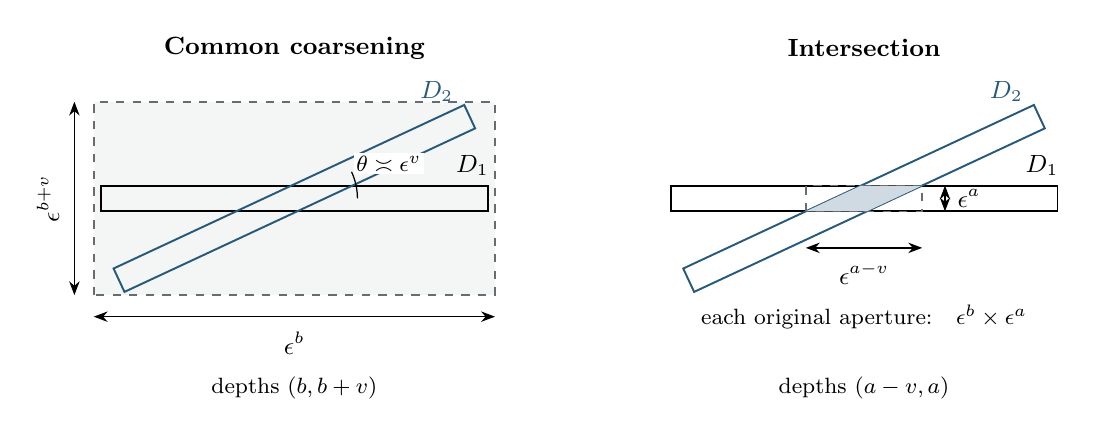
\begin{tikzpicture}[x=0.91cm,y=0.91cm,font=\small,
  aperture/.style={line width=0.7pt},
  comparison/.style={draw=figuregray,dashed,line width=0.6pt},
  dimension/.style={<->,>=Stealth,line width=0.45pt}]
  \begin{scope}[shift={(3.05,0)}]
    \node[font=\small\bfseries] at (0,2.10) {Common coarsening};
    \fill[figuregray!7] (-2.8,-1.35) rectangle (2.8,1.35);
    \draw[comparison] (-2.8,-1.35) rectangle (2.8,1.35);
    \draw[aperture] (-2.7,-0.18) rectangle (2.7,0.18);
    \begin{scope}[rotate=25]
      \draw[aperture,figureblue] (-2.7,-0.18) rectangle (2.7,0.18);
    \end{scope}
    \node[anchor=south west] at (2.12,0.19) {$D_1$};
    \node[anchor=south east,text=figureblue] at (2.35,1.22) {$D_2$};
    \draw[line width=0.45pt] (0.88,0) arc[start angle=0,end angle=25,radius=0.88];
    \node[anchor=west,font=\footnotesize,fill=white,inner sep=1pt]
      at (0.82,0.49) {$\theta\asymp\eps^v$};
    \draw[dimension] (-2.8,-1.65) -- (2.8,-1.65)
      node[midway,below=2pt] {$\eps^b$};
    \draw[dimension] (-3.07,-1.35) -- (-3.07,1.35)
      node[midway,above=2pt,sloped] {$\eps^{b+v}$};
    \node[font=\footnotesize] at (0,-2.65) {depths $(b,b+v)$};
  \end{scope}
  \begin{scope}[shift={(11.0,0)}]
    \node[font=\small\bfseries] at (0,2.10) {Intersection};
    \draw[aperture] (-2.7,-0.18) rectangle (2.7,0.18);
    \begin{scope}[rotate=25]
      \draw[aperture,figureblue] (-2.7,-0.18) rectangle (2.7,0.18);
    \end{scope}
    \fill[figureblue!22]
      (-0.81193,-0.18) -- (0.03991,-0.18) --
      (0.81193,0.18) -- (-0.03991,0.18) -- cycle;
    \draw[comparison] (-0.81193,-0.18) rectangle (0.81193,0.18);
    \node[anchor=south west] at (2.12,0.19) {$D_1$};
    \node[anchor=south east,text=figureblue] at (2.35,1.22) {$D_2$};
    \draw[dimension] (-0.81193,-0.69) -- (0.81193,-0.69)
      node[midway,below=2pt] {$\eps^{a-v}$};
    \draw[dimension] (1.13,-0.18) -- (1.13,0.18);
    \node[anchor=west,fill=white,inner sep=1pt] at (1.26,0) {$\eps^a$};
    \node[font=\footnotesize,align=center] at (0,-1.65)
      {each original aperture:\quad $\eps^b\times\eps^a$};
    \node[font=\footnotesize] at (0,-2.65) {depths $(a-v,a)$};
  \end{scope}
\end{tikzpicture}
\caption{Aperture geometry for two common-shape observations.
The centered schematic has $0<\eps<1$, $b\le a$ and
$0\le v\le a-b$, with angle $\theta\asymp\eps^v$.
Here $a=b+e$ in the notation of \eqref{eq:classical-rectangle-gain};
the two comparison rectangles give its weight gain.
The dashed common rectangle contains both apertures up to fixed factors;
the shaded intersection is contained in a rectangle with depths
$(a-v,a)$.  All indicated side lengths are orders of magnitude, and the
picture displays an interior value of $v$.  The same calculation applies
to the position column at duration $r$ after multiplying both side
lengths by $\eps^r$.}
\label{fig:aperture-geometry}
\end{figure}


\begin{proposition}[Least-aspect limiting extremizer]
\label{prop:least-aspect}
There exists a saturated sequence at duration one with $b=0$, endpoint
aspect $e=m$, and horizon $1+m$, where $m\ge0$ is the least aspect of
any such saturated sequence.  One may moreover require $Y_j$ conditional on $X_j$ to be homogeneous
for a prescribed countable list of finite pairs $(X_j,Y_j)$, provided
that for each fixed $j$ there is $0\le A_j<\infty$, independent of $\eps$,
such that $|\mathcal Y_j|\le\eps^{-A_j}$ for all sufficiently small $\eps$.
No cardinality bound is imposed on $X_j$, which may include the exact
particle $T$.
\end{proposition}
\begin{proof}
Choose systems whose normalized rates tend to $\betac$, split by narrow
shape bins, remove $b$ by localization, and normalize time.  Each
individual inner sequence now has a fixed finite aspect $e$; its
rate defect can be made arbitrarily small.  We need a bound for $e$
independent of which sequence was selected.

Sample two final labels independently given $T$, and let $D_1,D_2$ be
their root coarsenings of shape $(0,e)$.  If the rate defect is $\eta$,
then, since $S_1\le1+o(1)$ and $\betac\ge0$,
\[
 \Mut(T;D_j)\le(1-\gamma)e-\tau_L(T)+2+\eta+o(1).
\]
Tag their separation depth $v$ on a fixed mesh and use the common and
intersection labels above.  Conditional independence gives
\begin{align*}
 2e-(1+\gamma)\EE v-\tau_L(T)
 &\le\Mut(T;D_1,D_2)+O(\xi)+o(1)\\
 &\le2\big((1-\gamma)e-\tau_L(T)+2+\eta\big)
       -\big((1-\gamma)\EE v-\tau_L(T)\big)
       +O(\xi)+o(1).
\end{align*}
Indeed the information identity for the pair subtracts
$\Mut(D_1;D_2)$, which is at least the common-label entropy minus its
two determination errors.  That entropy is at least its particle
information, and the root test bounds the latter below by its weight
minus $\tau_L$.  The separation tag has entropy $o(1)$ at each fixed
mesh.  Rearrangement yields
\[
 2\gamma\EE(e-v)\le4+2\eta+O(\xi)+o(1).
\]
Thus a fixed $K=K_\gamma<\infty$ gives a positive, uniformly bounded
below probability of agreement within a bounded number of cells at
depth $(e-K)_+$.  For each $T$, maximize the conditional probability
of a coarse orientation cell.  The conditional collision probability
of two independent draws is at most a fixed constant times this
maximum.  This deterministic predictor therefore succeeds, to bounded
cell ambiguity, on an event of probability at least $c_\gamma>0$.
On that event the coarse orientation has conditional entropy $o(1)$
given $T$.  Binary splitting preserves a rate defect tending to zero
on this event.  Localization with $r=0$, $d=(e-K)_+$ produces a
conditional system with residual aspect at most $K$ and rate defect
tending to zero.  Uniform conditional deficit bounds justify selecting
one such system even when the conditioning cells are numerous.

It remains to take the least aspect.  The preceding construction,
followed by a diagonal, produces at least one saturated sequence with
bounded aspect and reduced horizon.  Let $m$ be the infimum of its
possible limiting aspects.  Choose such sequences with aspects
$e_j\to m$.  For the $j$th sequence choose its precision small enough
that its score defect, finite-menu errors, and the errors for the first
$j$ requested profiles are less than $1/j$.  Coarsen an endpoint of
aspect $e_j$ to aspect $m$ when $e_j\ge m$; if needed allow a depth error
$|e_j-m|$ before this coarsening.  The score loses at most
$C_\gamma|e_j-m|+o(1)$, whereas reducing the horizon to $1+m$ reduces
the subtracted root supremum.  The universal bound forces the resulting
diagonal to saturate.  For the homogeneity assertion, apply Lemma~\ref{lem:homogenization} to
finite initial lists of these pairs under the stated bounds on the child
alphabets, and choose their meshes and errors before the corresponding
precision.  Lemma~\ref{lem:profile-diagonal} then retains the countable
list.  In the applications below the children are finite tuples of grid
observations at fixed depths in bounded coordinates; the exact particle
and other unrestricted conditioning data occur only among the parents.
\end{proof}

\begin{proposition}[Saturated path and coherence]
\label{prop:saturated-path}
The sequence in Proposition~\ref{prop:least-aspect} can carry, on one
joint law of $(T,c)$, saturated observations $G_u$ at every positive
dyadic time $u\le1$.  Their shapes satisfy
\[
 b(1)=0,\quad a(1)=m,\quad
 b(r)\ge b(t),\quad a(r)+r\le a(t)+t\quad(r<t),
 \qquad e(u):=a(u)-b(u)\ge mu.
\]
They can be constructed so that
$\Ent(R_{e(u)}\mid T,C_u)=o(1)$.  There is a constant $K_\gamma$,
independent of $r,t$, for which the orientations at $r<t$ agree with
probability tending to one at every positive depth
\begin{equation}
 d<\min(e(r),e(t))-K_\gamma
       \bigl(|b(r)-b(t)|+|a(r)-a(t)|+t-r\bigr).
 \label{eq:classical-coherence}
\end{equation}
All statements refer to the inner $\eps$ limit with the times fixed.
\end{proposition}
\begin{proof}
On a finite dyadic mesh, work backwards from $1$ using
Lemma~\ref{lem:classical-localization} with $d=0$.  A composed predecessor
has minimum depth at least the later $b$ and maximum depth at most
the later $a$ plus the time difference.  Split its variable shape into
narrow bins and use Lemma~\ref{lem:classical-splitting} to preserve all
equalities already imposed.  Drop redundant labels.  Before making
this split, sample each incoming predecessor from its kernel given
$(T,C_r)$, independently of the previously retained finer time and
later labels.  This operation preserves its law with $(T,C_r)$ and
preserves the entire later joint law.  In particular the underlying
time variable is never resampled.

Subsequent finite binning and trimming introduce at most their normalized
entropy or relative-entropy cost into the averaged conditional mutual
information, by Lemma~\ref{lem:entropy-splitting}.  Retain typical parts
on which this cost and all finitely many score defects are bounded by
a common deterministic $q_\eps\to0$, using Markov thresholds fixed
before selecting parts.  The same lemma justifies the kernel
resampling with base $(T,C_r)$; at this stage no observation involving
a free replica is fixed.  Passing to finer finite meshes, and then to a diagonal,
gives the asserted common sequence and its dyadic shapes.  Shape bounds
follow from the fixed horizon.  A saturated observation at $u$,
localized with $r=d=0$ and normalized to duration one, has aspect
$e(u)/u$; minimality gives $e(u)\ge mu$.

Here are details of coherence.  Put
$D=|b(r)-b(t)|+|a(r)-a(t)|+t-r$.
Convert the observation at $t$ to the shape $(b(r),a(r))$ at $r$, using
its recorded frame rounded to the target precision and recording the
actual target cells.  Its additional conditional log-cardinality is at
most $C D+o(1)$.  To check this bound, rotate the old uncertainty into
the new frame: the tangent uncertainty entering the normal coordinate
has exponent at least
$b(t)+e(r)\ge a(r)-|b(t)-b(r)|$.  The other side-length changes cost
at most the absolute differences of the two depths.  Transport from
$C_t$ to $C_r$ adds $\eps^r$ times the velocity uncertainty, which has
the same bound in position units divided by $\eps^r$.  Counting the
finer cells in each resulting rectangle gives the stated estimate.
The weight changes by at most $2D$, and $S_t-S_r\le t-r+o(1)$.
Thus this converted test and the original test at $r$ have total
deficit at most $C_\gamma D+o(1)$ at duration $r$.

Call these two labels $D_1,D_2$, their common label $D_c$, and their
intersection label $D_i$.  They contain $C_r$, and their remaining
coordinates are deterministic functions of $T,C_r$ and their respective
orientations.  The resampling construction therefore gives
\[
 \Mut(D_1;D_2\mid T)\le S_r+o(1),\qquad
 \Ent(D_c\mid T)\ge S_r.
\]
The pair information identity and common-label determination imply
\begin{align*}
 \Mut(T;D_i)
 &\le\Mut(T;D_1)+\Mut(T;D_2)-\Ent(D_c)
                   +\Mut(D_1;D_2\mid T)+O(\xi)+o(1)\\
 &\le\Mut(T;D_1)+\Mut(T;D_2)-\Mut(T;D_c)+O(\xi)+o(1).
\end{align*}
Both $D_c,D_i$ have the same time $C_r$ and obey the original horizon.
Apply the universal score bound to each.  Their two time contributions
cancel the corresponding contributions in $D_1,D_2$, giving
\[
 2\gamma\EE(e(r)-v)\le C_\gamma D+O(\xi)+o(1).
\]
This inequality also holds on any separation event of fixed positive
limiting probability: binary splitting preserves the two original
saturations, and the extra conditional dependence costs only $o(1)$.
On the event $v\le d$ its left side is at least
$2\gamma(e(r)-d)$.  Choose $K_\gamma$ larger than the preceding
constant divided by $2\gamma$, and then let the angle mesh tend to
zero.  A positive limiting probability of separation at a depth in
\eqref{eq:classical-coherence} is impossible.

Apply the same comparison to two independent replicas of a single
label given $(T,C_u)$.  With $D=0$ they agree at every depth
$e(u)-\nu$, $\nu>0$, with probability tending to one.  For each base
value, a coarse cell and its bounded neighbors then contain all but
$o(1)$ of the conditional orientation mass on average.  Choose such a
cell deterministically from the base.  The entropy bound obtained by
separating this event from its complement is $o(1)$ at depth
$e(u)-\nu$; refining the orientation costs at most $\nu+o(1)$.
Let $\nu\downarrow0$.  This proves the asserted zero conditional
orientation entropy.
\end{proof}

\subsection{Isotropic tangents or a matched aspect}

\begin{proposition}[Tangent reduction]
\label{prop:isotropic-reduction}
One of the following alternatives holds for the least aspect $m$.
\begin{enumerate}
\item If $m=0$, there is a saturated sequence of duration and horizon
one, with isotropic endpoint $(b,a)=(0,0)$ and homogeneous conditional
time profile
\[
 \Ent(C_u\mid T)=su+o(1),\qquad 0\le u\le1,
 \quad 0\le s\le1.
\]
\item If $m>0$, the saturated path can be represented by a single
orientation $R$ with depth-$mu$ prefixes at time $u$, for every
$0<u\le1$, and
$\Ent(R_{mu}\mid T,C_u)=o(1)$.  Its shapes satisfy
\[
 e(u)=mu,\qquad b(u)\text{ is Lipschitz},\qquad
                 0\le-b'(u)\le1+m\quad\text{a.e.}
\]
There is $\kappa>0$ such that its limiting conditional orientation
entropies obey
\begin{equation}
 \Ent(R_{m(u+h)}\mid T,C_u)\ge\kappa h,
                  \qquad 0<u<u+h<1.
 \label{eq:orientation-growth}
\end{equation}
The alternatives and the positive lower bound persist after homogeneous
splittings that preserve the saturated path.
\end{enumerate}
\end{proposition}
\begin{proof}
The nesting inequalities make $b$ nonincreasing and $a(u)+u$
nondecreasing; extend them to their continuity points.  In particular
$e(u)+u$ is nondecreasing, so $e$ has bounded variation and its singular
distributional derivative is nonnegative.  Choose a common differentiability
point $x\in(0,1)$ for these functions.
Take dyadic $r<x<t$ with $\eta=t-r\downarrow0$ and with both distances
from $x$ comparable to $\eta$.  Differentiability gives uniform linear
approximations throughout $[r,t]$, with error $o(\eta)$.  Choose a finite
dyadic chain
\[
 r=u_0<u_1<\cdots<u_N=t
\]
whose largest interval length is $o(\eta)$, and put
\[
 D_j=|b(u_{j+1})-b(u_j)|+|a(u_{j+1})-a(u_j)|+u_{j+1}-u_j,
 \qquad D_{\max}=\max_jD_j.
\]
The uniform linear approximations give
$D_{\max}\le C\max_j(u_{j+1}-u_j)+o(\eta)=o(\eta)$.
Here the chain may become longer as $\eta\downarrow0$, but it is finite
and fixed at each inner small-parameter limit.

Let $e_{\min}=\min_j e(u_j)$ and choose a positive
$\delta_\eta=o(\eta)$.  Set
\[
 d=\bigl(e_{\min}-K_\gamma D_{\max}-\delta_\eta\bigr)_+.
\]
When $d>0$, it lies strictly below the coherence depth for every adjacent
pair in the chain.  Equation~\eqref{eq:classical-coherence} therefore
makes all their frames agree at depth $d$, up to bounded neighboring
cells, with probability tending to one.  Transitivity costs at most a
fixed number depending on this chain of neighboring cells, and the union
of its finitely many exceptional events still has probability tending
to zero.  The frame at $r$ is determined by $(T,C_r)$ to zero normalized
entropy at this depth.  The entropy ambiguity bound hence gives the same
determination for the terminal depth-$d$ frame.  If $d=0$, no orientation
information is required.

The uniform linear approximation for $e$ also gives
\[
 e(t)-e_{\min}\le\max(e'(x),0)\eta+o(\eta).
\]
Since $e_{\min}\ge0$, the definition of $d$ yields, in either case,
\[
 e(t)-d\le e(t)-e_{\min}+K_\gamma D_{\max}+\delta_\eta
       \le\max(e'(x),0)\eta+o(\eta).
\]
All depths, the chain, and its angular mesh are chosen before the inner
limit.  The depth loss is $K_\gamma D_{\max}$ at this one common depth;
the number of links enters only the zero-cost angular ambiguity.

Localize the terminal observation at $r$, using its common depth $b(t)$
and this $d$.  Its local horizon is $\eta+e(t)-d$.  Saturation and zero
conditional orientation entropy give saturated conditional systems.
With small parameter $\rho=\eps^\eta$, their duration is one and their
aspect is at most $\max(e'(x),0)+o(1)$.  All local coordinate bounds are
uniform, and their horizons stay bounded.  Minimality of $m$ therefore
implies $m\le\max(e'(x),0)$.  If $m>0$, this yields $e'(x)\ge m$
almost everywhere.  Since the singular derivative of $e$ is
nonnegative,
\[
 e(1)-e(u)\ge\int_u^1 e'(v)\,dv\ge m(1-u).
\]
Together with $e(u)\ge mu$ and $e(1)=m$, this proves $e(u)=mu$.
The original nesting inequalities now give
\[
 0\le b(r)-b(t)\le(1+m)(t-r),
\]
which proves the Lipschitz assertion and extends the path to every time.

We specify the selection of shrinking-scale limits, also for later use.
For the $j$th interval first fix its endpoints, its finite coherence
chain, and the first $j$ time-prefix fractions.  Homogenize their joint
and conditional probability bins, then choose the inner precision so
that all depth errors, normalized conditional entropies, uniform-bound
errors, and retained score deficits are less than $\eta_j/j^2$.
Use uniform typical sets before any further restriction.
The sum of the conditional deficits is then $o(\eta_j)$ in mean;
select typical localization cells with each required error
$o(\eta_j)$.  Only afterwards divide by $\eta_j$ and take the outer
diagonal.  This is an application of
Lemma~\ref{lem:profile-diagonal} with the error measured in the new
units.  No modulus of differentiability uniform over profiles is used.

 If $m=0$, use a common regular point with $e'\le0$ in the tangent
 construction above.  The set of such points has positive measure:
 otherwise $e'>0$ almost everywhere, and its nonnegative singular
 derivative would force $e(1)>e(u)\ge0$, contrary to $e(1)=0$.
 The nondecreasing $1$-Lipschitz homogeneous time profile $S_u$ is
 differentiable almost everywhere, so the point can also be chosen
 regular for $S$.  Put $s=S'(x)\in[0,1]$.  At this point the residual
 aspect just constructed is $o(\eta)$.

For the conditional time calculation, fix the finite list
$q=r+k\eta$ chosen above, and put $B=(T,C_r)$, $D_q=C_q$,
$d_q=S_q-S_r$, and $\ell=\log(1/\eps)$.  Let $\mathsf P$ be their
joint law with the localization label $J$, before its value is fixed.
The recorded conditional bins have one error $\omega_\eps=o(\eta)$
for this list outside probability $o(1)$, while the preceding parameter
choice gives $\Ent^{\mathsf P}(J\mid B)=o(\eta)$.  At sampled values,
\[
 -\ell^{-1}\log\mathsf P(D_q\mid B,J)
 +\ell^{-1}\log\mathsf P(D_q\mid B)
 =\ell^{-1}\log
       \frac{\mathsf P(J\mid B)}{\mathsf P(J\mid B,D_q)}.
\]
The two nonnegative $J$ surprises on the right have means at most
$\Ent^{\mathsf P}(J\mid B)$.  Choose $\delta_\eps=o(\eta)$ with
$\Ent^{\mathsf P}(J\mid B)/\delta_\eps\to0$ and trim them by Markov's
inequality.  Intersecting with the recorded bins leaves an event $E$ of
probability $1-o(1)$ on which, simultaneously for the listed $q$,
\[
 -\ell^{-1}\log\mathsf P(J\mid B)\le\delta_\eps,\qquad
 \left|-\ell^{-1}\log\mathsf P(D_q\mid B,J)-d_q\right|
       \le\alpha_\eps:=\omega_\eps+\delta_\eps=o(\eta).
\]
The list is fixed before choosing the inner precision; its errors and
exceptional masses are put under one deterministic vanishing envelope
before the lists grow along the preceding diagonal.

Put $\mathsf P^E=\mathsf P(\,\cdot\mid E)$.  Conditional relative
entropy gives
\[
 \Ent^{\mathsf P^E}(J\mid B)
 \le\mathbb E_{\mathsf P^E}[-\ell^{-1}\log\mathsf P(J\mid B)]
 \le\delta_\eps=o(\eta).
\]
Since $J$ records $R_d$, this also bounds the orientation cost under
$\mathsf P^E$.  The binary tag $\boldsymbol1_E$ costs
$O(1/\ell)=o(\eta)$.  Lemma~\ref{lem:classical-splitting}, the original
$o(\eta)$ deficits, and the common lower bound $-o(\eta)$ for the
complementary deficits give $o(\eta)$ deficits on $\mathsf P^E$.
Localization of this law has conditional laws
$\mathsf Q_j=\mathsf P(\,\cdot\mid E,J=j)$, followed by the known
$J$-dependent coordinate change.  The shrinking-scale selection above
therefore gives a set of $\mathsf P^E_J$-mass $1-o(1)$ on which the
required local deficits are $o(\eta)$ under the same finite envelope.

Choose one $\lambda_\eps\downarrow0$ with
$\log(1/\lambda_\eps)=o(\eta\ell)$, using $\eta\ell\to\infty$.
Apply Lemma~\ref{lem:typical-conditioning} to the event $E$, with
$C=J$, $X=(B,J)$, $Y=D_q$, and all three exceptional thresholds
equal to $\lambda_\eps$.
Outside $\mathsf P^E_J$-mass at most $\lambda_\eps$, it gives
\[
 \mathsf Q_j\le[\mathsf P(E)\lambda_\eps]^{-1}\mathsf P_j,
 \qquad \mathsf P_j=\mathsf P(\,\cdot\mid J=j).
\]
On $J=j$, conditioning on $X$ is conditioning on $B$, and the bin
on $E$ is for $\mathsf P(D_q\mid B,J)=\mathsf P_j(D_q\mid B)$.
The lemma's entropy and surprise conclusions therefore give
\[
 \begin{gathered}
 \Omega_\eps:=
 \alpha_\eps+\ell^{-1}\log\frac1{\mathsf P(E)\lambda_\eps^2}
       =o(\eta),\\
 \left|\Ent^{\mathsf Q_j}(D_q\mid B)-d_q\right|\le\Omega_\eps,\qquad
 \mathsf Q_j\!\left\{
 \left|-\ell^{-1}\log\mathsf Q_j(D_q\mid B)-d_q\right|
       >\Omega_\eps\right\}\le2\lambda_\eps .
 \end{gathered}
\]
These are uniform over the retained $j$ and the fixed finite list;
the finite union bound is absorbed by the same diagonal.  No original
cell probability enters the error envelope.

Intersect these cells with the typical localization cells above.
Since $C_r$ is fixed by $J$ and the local time grids correspond to
$C_q$ up to bounded ambiguity, the estimates are conditional on the
local particle.  Differentiability gives $(S_q-S_r)/\eta=ks+o(1)$.
The residual aspect and excess horizon are $o(1)$ in the new units;
coarsen these vanishing depth errors and apply the universal bound to
recover a saturated isotropic sequence.  Increasing the finite prefix
lists gives the homogeneous linear time profile and proves the first
alternative.

Suppose henceforth $m>0$.  Fix a dyadic $u>0$.  On a sufficiently fine
finite chain from $u$ to $1$, coherence and the Lipschitz width bounds
identify all frames at every depth strictly below $mu$.  The terminal
orientation $R$ thus determines the frame at $u$ at that precision.
Let the gap from $mu$ tend to zero.  Both the old and new rectangles
then determine each other with vanishing log-cardinality error;
recording the same data in the endpoint-prefix frame preserves its
score.  Taking a diagonal over dyadic $u$, and then using Lipschitz
interpolation of the widths and time grids, supplies the common-prefix
representation at every $u$.

Finally, if no $\kappa>0$ satisfies \eqref{eq:orientation-growth},
there are fixed intervals $(u_j,u_j+h_j)$, chosen after their inner
limits, with
\[
 h_j^{-1}\Ent(R_{m(u_j+h_j)}\mid T,C_{u_j})\longrightarrow0.
\]
Apply Lemma~\ref{lem:classical-localization} to the saturated observation
at $u_j+h_j$, with $r=u_j$, $b=b(u_j+h_j)$, and
$d=e(u_j+h_j)$.  Its conditional final shape is exactly isotropic and
its local horizon is $h_j$.  The error $2\zeta$ in
\eqref{eq:classical-local-first} is $o(h_j)$.  The other composition
errors are made $o(h_j)$ by first fixing the interval and then choosing
the inner precision.  The local deficits consequently have mean
$o(h_j)$ and a uniform lower bound of the same order.  Select a local
system with deficit $o(h_j)$ and replace $\eps$ by $\eps^{h_j}$.
This produces a saturated isotropic sequence of horizon one, contrary
to $m>0$.  This contradiction proves the uniform positive constant.
It uses neither a positive lower bound for $h_j$ nor one for
$u_j$: both are fixed positive numbers at their own inner stage.

The same arguments apply after any homogeneous splitting preserving
the path's scores.  Such a path is still a least-aspect extremizer, so
the final contradiction again supplies a positive constant.  One can
also fix a projective orientation chart by a finite split.  In that
chart use rows $(1,0)$ and $(-R,1)$, with bounded slope $R$ and nested
slope prefixes.  The row frame and orthogonal frame have bounded
condition number, angular and slope precisions are comparable, and
the resulting rectangle observations differ by bounded covering
multiplicities.  All conclusions therefore hold in this row convention.
\end{proof}

\begin{remark}[Homogeneous profiles for subsequent local arguments]
\label{rem:classical-profile-inheritance}
In either alternative of Proposition~\ref{prop:isotropic-reduction},
one may first impose a fixed finite list of pairs $(X_j,Y_j)$ satisfying
$|\mathcal Y_j|\le\eps^{-A_j}$ for fixed $0\le A_j<\infty$ and all
sufficiently small $\eps$.  The children may be joint grid observations
or geometric prefixes.  No cardinality bound is imposed on the
conditioning variables $X_j$, which may include $T$.
  Apply
Lemma~\ref{lem:homogenization} and
Lemma~\ref{lem:classical-splitting}, select a saturated homogeneous
component, and only then define its limiting profiles and choose a
differentiability or trace point.  The profiles need not equal those
before this initial splitting.  The positive constant in
\eqref{eq:orientation-growth} is obtained for the selected component
by the same least-aspect contradiction.

To spell out the later inheritance, suppose homogeneous probability
bins for a parent $P$ and a refinement $Q$ have exponents $d_P,d_Q$
with error $\eta$; both may be conditional on an additional base $W$,
including the exact particle.
Here $d_P$ is the exponent for the child $P$, and $d_Q$ is the exponent
for the joint child $(P,Q)$, identified with $Q$ when $Q$ already records
$P$; both children are conditional on $W$.  If the exact particle is
present, it belongs to $W$.
  On their common uniform typical set,
ratios of joint and parent masses give
\[
 \Pr(Q=q\mid P=p,W=w)
       \le\eps^{d_Q-d_P-2\eta},\qquad
 \#\{q:\ (p,q,w)\text{ retained}\}
       \le\eps^{-(d_Q-d_P)-2\eta}.
\]
These are respectively an upper conditional mass and an upper retained
support count; they are stronger than an averaged entropy inequality.
If a subsequent normalized law $\nu$ obeys
$\nu\le\eps^{-\theta}\mu$, discard parent values whose marginal
likelihood $\nu_{P,W}/\mu_{P,W}$ is below $\eps^\lambda$.  Their
$\nu$-probability is at most $\eps^\lambda$, and on the remaining
parents the conditional mass bound loses at most $\theta+\lambda$
in its exponent.  Support counts are inherited under restriction.
The conditional relative-entropy identity in
Lemma~\ref{lem:homogenization} supplies the corresponding lower entropy
bound with loss $\theta$.  There is no factor depending on the number
of parent values.  Repeat this operation for the fixed finite list,
then take a diagonal.  For a block of length $h$, choose
$\eta,\theta,\lambda=o(h)$ at its inner stage before using
$\rho=\eps^h$ as the small parameter.  Cap regularization may be imposed
at the same stage to retain the root bound
\eqref{eq:classical-cap-bounds} under these operations.
\end{remark}

\section{Exclusion of isotropic extremizers}
\label{sec:isotropic}

We exclude the isotropic alternative in
Proposition~\ref{prop:isotropic-reduction}. The argument has two
geometric steps. Three sufficiently separated slopes would force
more point entropy than saturation allows, so one can retain a slope
population in a thin strip. That strip supplies an earlier anisotropic aperture;
a two-slope projection estimate in the remaining block then forces
a conditional time rate greater than one. Throughout both changes
of scale we retain uniform conditional probability bounds on particle
fibers, as well as the corresponding entropy inequalities.

\begin{proposition}[Isotropic exclusion]
\label{prop:isotropic-exclusion}
Suppose that $0<\gamma<1$ and that the classical universal growth rate satisfies
$\beta>\gamma$. There is no saturated isotropic system of duration and horizon
$1$ furnished by Proposition~\ref{prop:isotropic-reduction}, with homogeneous
conditional time profile $\Ent(C_u\mid T)=su$, $0\leq u\leq1$.
\end{proposition}

Here and below, a limiting assertion about homogeneous probabilities is used
on the trimmed laws of Lemma~\ref{lem:homogenization}. In particular, it supplies
uniform probability bounds on the retained joint population. An exceptional
set of small probability in an untrimmed conditional law is not treated as a
uniform probability bound. We give the finite estimates that implement this
distinction in the present argument.

\subsection{Finite incidence counts and regular increments}

In the next two elementary estimates $\rho$ is a mesh size, and all coordinates
belong to a fixed bounded set. Constants may depend on that set, but not on
$\rho$. A point cell in dimension $d+1$ has coordinates $(c,x)\in\RR\times
\RR^d$, and a slope bin has representative $v\in\RR^d$ and diameter $O(\rho)$.
The intercept map is
\[
 \pi_v(c,x)=x-cv.
\]

\begin{lemma}[Counting intercepts on retained fibers]
\label{lem:isotropic-intercepts}
Suppose an incidence population uses at most $N$ point cells. For every
retained exact particle and slope bin incident to it, suppose there are at
least $m$ distinct retained time children in the same base cell and slope bin.
Suppose further that these children lie on one line of true slope within
$O(\rho)$ of the bin representative. Then, for each slope bin, all its retained
incidences use at most $CN/m$ intercept cells of side $\rho$.
\end{lemma}

\begin{proof}
Fix the slope bin. A particle's intercept $x-cv$ varies by $O(\rho)$ along its
retained children. Its distinct time children give distinct point cells.
For every occupied intercept cell $b$, choose one particle witnessing an
incidence in $b$. The particle's $m$ point cells have intercepts in a fixed
bounded enlargement of $b$. A point cell can belong to the enlargements of
only $C$ intercept cells, since $v$ is fixed. Counting the pairs consisting of
an occupied intercept cell and one of these witnesses gives $m\#\{b\}\leq CN$.
This counts point cells, and imposes no bound on the number or entropy of exact
particles. The estimate concerns the population before replica labels are
fixed; its support upper bound continues to hold on every subsequent subset.
\end{proof}

We will use the following explicit form of the star calculation in
Theorem~\ref{thm:finite-conditioning}. Let $q$ be a normalized point--slope law
with actual marginals $\mu,\nu$, and suppose
\begin{equation}
 q(p,v)\leq K\mu(p)\nu(v),\qquad \mu(p)\leq M^{-1}.
 \label{eq:isotropic-pair-comparison}
\end{equation}
Sample $r$ slopes independently conditional on $p$. The resulting law $q_r$
satisfies both comparisons
\begin{align}
 q_r(p,v_1,\ldots,v_r)&\leq K^r\mu(p)\prod_{i=1}^r\nu(v_i),
 \label{eq:isotropic-star-comparison}\\
 q_r(p,v_1,\ldots,v_r)&\leq
 K^{r-1}q(p,v_j)\prod_{i\ne j}\nu(v_i)\quad(1\leq j\leq r).
 \label{eq:isotropic-one-pair-comparison}
\end{align}
These follow by multiplying $q(v_i\mid p)\leq K\nu(v_i)$, keeping one factor
unestimated for the second inequality. If $\lambda$ is the slope-tuple marginal,
then the tuples on which $\lambda/\prod_i\nu(v_i)<L^{-1}$ have
$\lambda$-mass at most $L^{-1}$, by summing against the product probability.
Outside that set,
\begin{equation}
 q_r(p\mid v_1,\ldots,v_r)\leq K^r L\mu(p).
 \label{eq:isotropic-pinning}
\end{equation}
Thus fixing a typical tuple leaves at least $M/(K^rL)$ point cells. An event
of independent slope probability $\eta$ has star probability at most $K^r\eta$.
All applications below first trim pairs, discard point fibers of inadequate
retention, and replace comparison marginals by the actual retained marginals
using Theorem~\ref{thm:finite-conditioning}. Consequently
\eqref{eq:isotropic-pair-comparison} holds for the normalized retained law.
The fixed labels will always be precisely these two or three slope replicas;
no cyclic incidence configuration is used.

\begin{lemma}[Two elementary projection inequalities]
\label{lem:isotropic-grid-projections}
Let $E$ be a set of occupied $\rho$-cells in a fixed bounded region.
\begin{enumerate}
\item In $\RR^3$, let $v_1,v_2,v_3\in\RR^2$ be bounded slopes and put
$D=\abs{\det((1,v_1),(1,v_2),(1,v_3))}>0$. If $\pi_{v_i}(E)$ uses at most
$N_i$ cells, with bounded enlargements permitted, then
\begin{equation}
 \abs E^2\leq C D^{-6}N_1N_2N_3.
 \label{eq:isotropic-lw}
\end{equation}
\item In $\RR^2$, for two bounded scalar slopes $v_1,v_2$ with
$\abs{v_1-v_2}\geq\rho^a$, if their intercepts use at most $N_1,N_2$ cells,
then
\begin{equation}
 \abs E\leq C\rho^{-2a}N_1N_2.
 \label{eq:isotropic-two-projections}
\end{equation}
\end{enumerate}
\end{lemma}

\begin{proof}
For the first assertion choose a witness point in each occupied cell, and
let $U$ have columns $(1,v_i)$. Replace each $U^{-1}z$ by its $\rho$-grid cell,
obtaining a finite grid set $Y$. Since $\norm U\leq C$, each cell of $Y$
accounts for at most $C$ original cells, so $\abs E\leq C\abs Y$.
The map $\pi_{v_i}U$ annihilates the $i$th coordinate. On the other two
coordinates it is an invertible matrix of determinant of absolute value $D$
and inverse norm at most $C/D$. Thus each original intercept cell accounts
for at most $CD^{-2}$ cells of the coordinate projection of $Y$ omitting
coordinate $i$. Rounding $U^{-1}z$ adds only $O(\rho)$ to its intercept,
because $\pi_{v_i}U$ has bounded norm.

For completeness, the discrete Loomis--Whitney inequality
\citep{LoomisWhitney1949} used here is
\[
 \abs Y^2\leq\abs{\pi_{12}Y}\abs{\pi_{13}Y}\abs{\pi_{23}Y}.
\]
To see it, write $f_{ij}$ for the indicators of the three projected sets.
The sum
\[
 \sum_{x,y,z}f_{12}(x,y)f_{13}(x,z)f_{23}(y,z)
\]
majorizes $\abs Y$.
Cauchy--Schwarz first in $z$ bounds this sum by
$\sum_{x,y}f_{12}(x,y)\sqrt{b_x c_y}$, where
$b_x=\sum_z f_{13}(x,z)$ and $c_y=\sum_z f_{23}(y,z)$.
Cauchy--Schwarz in $(x,y)$ bounds its square by
$\abs{\pi_{12}Y}(\sum_x b_x)(\sum_y c_y)$.
Combining the three projection bounds proves \eqref{eq:isotropic-lw}.
For the second assertion, the inverse of
$(c,x)\mapsto(x-v_1c,x-v_2c)$ has norm at most $C\rho^{-a}$.
Each pair of intercept cells therefore meets at most $C\rho^{-2a}$ point
cells. Summing over the pairs proves \eqref{eq:isotropic-two-projections}.
\end{proof}

Here is the scale-selection fact needed twice below. Let $F_u$, $0\leq u\leq1$,
be a filtration and let $X_h$ have normalized entropy at most $Dh$. For an
optional fixed conditioning variable $Z$, put
$g_h(u)=\Mut(X_h;F_u\mid Z)$. Nestedness and the chain rule give
\begin{equation}
 \int_0^{1-h}\Mut(X_h;F_{u+h}\mid Z,F_u)\,du
 =\int_0^{1-h}(g_h(u+h)-g_h(u))\,du
 \leq h\Ent(X_h\mid Z)\leq Dh^2.
 \label{eq:isotropic-integrated-information}
\end{equation}
The middle inequality follows by canceling the two integrals on their common
interval. For a sequence $h_j$ with $\sum_j\sqrt{h_j}<\infty$, Markov's
inequality and the elementary Borel--Cantelli argument show that, for almost
every $u$, the integrand divided by $h_j$ is at most $\sqrt{h_j}$ eventually.
The same points may be required to be differentiability points of any fixed
finite collection of Lipschitz entropy profiles.

Our anchored observations are nested only to bounded ambiguity. Formula
\eqref{eq:isotropic-integrated-information} is applied to their limiting
profiles. Its exact finite counterpart can instead use the nested dyadic
cells of the physical point $(c,A+cV)$: at every fixed depth $u$ these and
$(C_u,[A+C_uV]_u)$ determine each other with a bounded number of possibilities.
All entropy differences and conditional mutual informations consequently
differ by $O(1/\log(1/\eps))$. This error is taken to zero before $h$.

\subsection{The isotropic entropy bounds}

For a vector $Y$, write $[Y]_d$ or $Y_d$ for its isotropic grid
observation at scale $\eps^d$.
Assume the system in Proposition~\ref{prop:isotropic-exclusion} exists. Write
\[
 O_u=(C_u,[A+C_uV]_u),\qquad O=O_1,\qquad
 \alpha=2-2s+\beta.
\]
The exact particle $T$ determines $A,V$. In an anchored observation it leaves
only the time label random, so $\Ent(O_u\mid T)=su$. Write $\tau$ for the
root supremum, equivalently its uniformized cap level in the limiting system.
The terminal weight is zero. Saturation therefore gives
\begin{equation}
 \beta=-\Mut(T;O)+2s-\tau=3s-\Ent(O)-\tau.
 \label{eq:isotropic-terminal-score}
\end{equation}
Since $\tau\geq0$ and $\Mut(T;O)\geq0$, we have $\beta\leq2s$ and
\begin{equation}
 \Ent(O)\leq3s-\beta,\qquad
 \Ent(V_d\mid O)\geq\alpha d\quad(0\leq d\leq1).
 \label{eq:isotropic-alpha}
\end{equation}
To prove the second inequality, test at duration $1-d$ with velocity depths
$(d,d)$ and position depths $(1,1)$. Denote this observation by $\widetilde O$.
Its weight is $2d$, and its conditional time entropy is $s(1-d)$.
Universality and \eqref{eq:isotropic-terminal-score} imply
\[
 \Mut(T;\widetilde O)-\Mut(T;O)\geq(2-2s+\beta)d.
\]
The pair $(O,V_d)$ determines $\widetilde O$ to bounded ambiguity: transport
over a time displacement $O(\eps^{1-d})$ with velocity uncertainty
$O(\eps^d)$ has position error $O(\eps)$. The information difference is
therefore at most $\Ent(V_d\mid O)$ in the limit. At $d=1$ the identical
inequality follows from the definition of the root supremum at duration zero.
Notice that $\alpha\geq\beta>0$.

Homogenize jointly $O$, $V_d$, and their conditioning variables, for the
finite lists of depths used below. Formula~\eqref{eq:isotropic-alpha} then
means, on the trimmed joint population,
\begin{equation}
 \PP(V_d=q\mid O=o)\leq\eps^{\alpha d-\eta}
 \label{eq:isotropic-velocity-mass}
\end{equation}
with arbitrarily small $\eta>0$ after taking the inner limit. Indeed the
conditional probability exponent is the difference of the homogeneous
joint and marginal exponents, and that difference is at least $\alpha d$.
The same construction records the time probabilities conditional on the
exact particle. It is legitimate on saturated homogeneous parts by the
splitting and cap conclusions of Proposition~\ref{prop:isotropic-reduction}.

\subsection{Concentration of slopes in a thin strip}

The profile $u\mapsto\Ent(O_u)$ is nondecreasing and $3$-Lipschitz, starts at
zero, and has endpoint at most $3s-\beta$. There is consequently a set of
positive measure of regular points $k\in(0,1)$ with
\begin{equation}
 p:=\partial_k\Ent(O_k)<3s-\beta/2.
 \label{eq:isotropic-low-increment}
\end{equation}
Choose such a point satisfying \eqref{eq:isotropic-integrated-information}
with $X_h=V_h$, whose entropy is at most $2h$. Along a sequence $h\downarrow0$,
\begin{equation}
 \Ent(O_{k+h}\mid O_k)=(p+o(1))h,\qquad
 \Mut(V_h;O_{k+h}\mid O_k)=o(h).
 \label{eq:isotropic-first-increment}
\end{equation}

Inside a typical $O_k$-cell translate time and position to the cell center
and dilate both by $\eps^{-k}$. Put $\rho=\eps^h$, and call the child point
observation $P$. Bounded changes from anchored to physical point cells do
not affect any exponent. Homogeneity, the conditional fiber rule, and
Lemma~\ref{lem:zero-information}, followed by the actual-marginal conclusion
of Theorem~\ref{thm:finite-conditioning}, give a normalized retained pair law
$q(P,V_h)$ satisfying the following bounds, with $e=e(h)\to0$:
\begin{align}
 \#\supp P&\leq\rho^{-(p+e)},&
 \mu(P=z)&\leq\rho^{p-e},&
 q&\leq\rho^{-e}\mu\otimes\nu.
 \label{eq:isotropic-first-graph}
\end{align}
These conclusions hold outside base cells of probability tending to zero.
One may enlarge $e(h)$ to absorb all fixed numerical constants and all
$o(1)$ errors in \eqref{eq:isotropic-first-increment}. To be explicit about
the conditioning: the mean information in block units tends to zero; discard
base cells where it exceeds its square root, apply the likelihood-ratio
truncation in each remaining cell, and discard point fibers losing more than
half their mass. Homogeneous joint and marginal bounds then supply the two
point estimates in \eqref{eq:isotropic-first-graph}. This procedure introduces
only another quantity tending to zero into $e$.

We also trim on the exact particle fibers before sampling replicas. A retained
time child, conditional on $T,C_k$ in the original base law, has probability
at most $\rho^{s-e}$. Lift all pair restrictions to that law, and discard
particle fibers whose conditional retention there is below $\rho^e$.
If the pair restrictions have total retention $m_0$, these discarded fibers
have normalized retained mass at most $\rho^e/m_0$, by
\eqref{eq:retention-fibers}. Here $m_0$ is bounded below before this step;
more generally a subpower lower bound is absorbed by increasing $e$.
Each remaining particle has at least $\rho^{-s+2e}$ distinct retained time
children, by dividing its retained mass by the original child mass bound.
Given $T,C_k$, the anchored base observation is fixed. Thus this is a statement
in the very same base cell used for $P$; no particle entropy bound is involved.
For a slope bin of size $\rho$, all these points have intercept within $O(\rho)$
of the particle's intercept. Lemma~\ref{lem:isotropic-intercepts} gives
\begin{equation}
 \#\pi_v(\text{retained neighbors of }v)
 \leq C\rho^{-(p-s+3e)}.
 \label{eq:isotropic-first-intercepts}
\end{equation}
Apply one final simultaneous marginal core to this pruned law. Its retention
is at least one half, by Lemma~\ref{lem:marginal-core}, and the pair comparison
again uses its actual point and slope marginals. Increasing $e$ absorbs the
finite factors, so \eqref{eq:isotropic-first-graph} and
\eqref{eq:isotropic-first-intercepts} hold together for this final pair law.
The core need not preserve the rich particle fibers: the intercept support
bound was established before it, and survives by support inclusion. Use
this same order of operations in the two-replica application below.

Fix $\vartheta>0$ so small that $12\vartheta<\beta/8$. We claim that, in every retained
base cell, some strip of thickness $C\rho^\vartheta$ has slope mass at least
$\rho^{5e}$, after enlarging $e(h)\to0$ once more. If all such strips had
mass less than $\rho^{5e}$, two independent slopes would have distance at least
$\rho^\vartheta$ except with probability $C\rho^{5e}$; a ball of that radius is
contained in a strip of comparable thickness. Conditional on the first two,
the third would lie at distance at least $\rho^\vartheta$ from their line except
with the same probability. Hence, outside an independent event of probability
$C\rho^{5e}$,
\[
 \abs{\det((1,v_1),(1,v_2),(1,v_3))}\geq\rho^{2\vartheta}.
\]
For the three-replica star, \eqref{eq:isotropic-star-comparison} bounds the
exceptional probability by $C\rho^{2e}$. Choose $L=\rho^{-e}$ in
\eqref{eq:isotropic-pinning}. A good tuple then leaves a point population of
at least $\rho^{-p+5e}$ cells, and each projection has the support bound
\eqref{eq:isotropic-first-intercepts}. Lemma~\ref{lem:isotropic-grid-projections}
implies
\[
 2p-10e\leq3(p-s+3e)+12\vartheta+o_{\rho\to0}(1),
 \qquad\text{hence}\qquad
 p\geq3s-12\vartheta-19e-o_{\rho\to0}(1).
\]
This contradicts \eqref{eq:isotropic-low-increment} for all sufficiently small
$h$, with $\rho$ taken sufficiently small afterwards. We take $e>0$ even
when an error vanishes, so that the exceptional probabilities above tend to
zero in this inner limit.

Choose one such strip measurably in each base cell, using a finite grid menu
with bounded enlargement, and restrict incidences to it. The total retention
is at least $\rho^{5e}$ times the mass of the retained base cells. No strip
index is fixed globally: its index is a function of $O_k$ and will be included
in the earlier test through that base label. With
\begin{equation}
 l=\vartheta h,
 \qquad \abs{V\cdot n(O_k)-w(O_k)}\leq C\eps^l,
 \label{eq:isotropic-strip}
\end{equation}
round the unit normal and offset at precision $\eps^l$. This changes $C$ only.
The Radon--Nikodym bound for the restriction is $\eps^{-O(eh)}$.
Since $\vartheta$ is fixed and $e(h)\to0$, its normalized logarithmic cost is
$o(l)$.

The bins for $O$, the required $V_d$, and the particle-conditional time
probabilities are trimmed before this restriction. Lemma~\ref{lem:homogenization}
and its conditional retention rule
therefore preserve their exponents with errors $o(l)$, including the
particle-conditional time exponents and \eqref{eq:isotropic-velocity-mass}.
The absolute root cap bound gives $\tau_{\rm new}\leq\tau+o(l)$.
The terminal numerator before subtraction of $\tau$ changes by $o(l)$, because
its observation and conditional time exponents were recorded. Consequently
the new terminal score is at least $\beta-o(l)$, and universality bounds it
above by $\beta+o(l)$. We henceforth use this retained law and its own root
supremum; its terminal score is $\beta+o(l)$.

\subsection{An earlier anisotropic observation}

Take $h$ small enough that $k<1-l$, and put $a=1-l$. In the frame with normal
$n=n(O_k)$ and tangent $n^\perp$, form
\begin{equation}
 B=\bigl(O_k,O_a,[(A+C_aV)\cdot n]_1\bigr).
 \label{eq:isotropic-earlier-test}
\end{equation}
The coarse observation $O_a$ locates tangent position to depth $a$; its
normal position is additionally located to depth $1$. The strip supplies
normal velocity to depth $l$, and tangent velocity is bounded. The rounded
frame is known to depth $l$. Thus $B$, with boundedly many additional data
cells if necessary, is an admissible aperture with velocity depths $(0,l)$,
duration $a$, horizon $1$, and weight $(1-\gamma)l$.

It is determined by $O$ to bounded ambiguity. Indeed $O$ coarsens to $O_k,O_a$
to bounded ambiguity, hence determines the chosen strip up to the same fixed
number of choices. For its fine normal position use
\begin{equation}
 (A+C_aV)\cdot n=(A+C_1V)\cdot n+(C_a-C_1)w+O(\eps),
 \label{eq:isotropic-normal-transport}
\end{equation}
where the error is bounded by
$C\eps^a\eps^l=C\eps$. Conversely every component of the anchored $B$ is
fixed by $(T,C_a)$, since $C_a$ fixes $C_k$. In particular,
\begin{equation}
 \Ent(O\mid T,B)=sl+o(l).
 \label{eq:isotropic-last-time}
\end{equation}
The conditional time profile on the retained law follows from the ratios of
the recorded probabilities at depths $a$ and $1$; the strip restriction costs
$o(l)$ on typical particle fibers. Adjoining standard data cells to $B$
uses deterministic functions of $(T,C_a)$ and leaves this argument unchanged.

We prove the information saving
\begin{equation}
 \Mut(T;O)-\Mut(T;B)\geq sl-o(l).
 \label{eq:isotropic-information-saving}
\end{equation}
The main point is a lower bound for the last block's joint time and tangent
position entropy.

\subsection{Slope bounds inside the last block}

For $0\leq u\leq1$ let $F_u$ record, in addition to $B$, time to depth
$a+ul$ and tangent position at that time to the same depth. Within a $B$-cell
translate time and tangent position to their depth-$a$ centers and dilate
both by $\eps^{-a}$. The resulting coordinates are bounded, the new mesh
parameter is $\rho_*=\eps^l$, and the tangent slope
$X=V\cdot n^\perp$ remains bounded. The filtration $F_u$ has capacity $2$
per unit depth. Its base $F_0$ adds at most bounded information to $B$, and
$F_1$ is determined by $(O,B)$ to bounded ambiguity. Given $T,B$, its
conditional entropy profile is $su+o(1)$ in block units, because its new data
are fixed by the particle and the time cell.

For each fixed $d\in(0,1]$ and each fixed filtration depth $u$, the retained
conditional tangent slope law satisfies
\begin{equation}
 \PP\bigl(X\in J\mid B,F_u\bigr)
 \leq \rho_*^{\alpha d-o(1)}
 \quad\text{for intervals }J\text{ of length }\rho_*^d.
 \label{eq:isotropic-inherited-tangent}
\end{equation}
Here, as throughout, the inequality is uniform on a further trimmed
subprobability, followed by normalization on fibers of subpower retention.
We verify this transfer, since a bare conditional entropy inequality would
not suffice.

First apply \eqref{eq:isotropic-velocity-mass} at velocity depth $dl$ on the
jointly trimmed law. Adjoin the finite list of labels $(B,F_u)$ to $O$.
Each such list has at most $K$ possible values given $O$, where $K$ is fixed
when the list is fixed. For a positive tolerance $\zeta$, discard realized
values whose conditional likelihood given $O$ is below $\rho_*^\zeta$.
Their total probability is at most $K\rho_*^\zeta$. On the remaining values,
conditioning on the adjoined label multiplies a conditional velocity-bin
probability by at most $\rho_*^{-\zeta}$. More explicitly, write
$\kappa_h=O(e(h)/\vartheta)$ for an upper bound on all prior restriction costs
in last-block units. Whenever a retained subprobability has mass at least
$\rho_*^{\kappa_h}$, discard conditioning fibers whose retention is below
$\rho_*^{\kappa_h+\zeta}$. Formula~\eqref{eq:retention-fibers} bounds their
normalized retained mass by $\rho_*^\zeta$; normalization costs at most
$\kappa_h+\zeta$ in the conditional exponent. For the fixed finite number
of such operations, the total extra loss is $C\kappa_h+C\zeta$.
It tends to zero by first taking the inner limit, then $h\downarrow0$ and
$\zeta\downarrow0$. It incurs no factor involving the number of $O$-cells
or $B$-cells.

For a fixed $B$-cell, its normal strip has thickness $O(\eps^l)$. Its
intersection with a tangent interval of length $\eps^{dl}$ meets only $C$
velocity grid cells of depth $dl$, since $d\leq1$. Thus the same uniform
upper bound holds for this tangent interval conditional on $O,B,F_u$.
Averaging over compatible $O$-labels gives
\eqref{eq:isotropic-inherited-tangent}, with the explicit extra exponent
loss $\zeta$ and the retention losses. Taking those losses to zero proves
the asserted form. Every bound is imposed on the retained joint population
before averaging; no exponentially small bound for untrimmed exceptional
probabilities is needed.

We now make the order of limits precise. Fix $\vartheta$ first. Choose the regular
sequence $h\downarrow0$ above. For each fixed $h$ record the finite lists of
$O,V_d$, and particle-conditional time bins before the strip choice.
Construct $B,F_u$ and perform the transfer just proved after choosing the
strip. The later increment binnings are performed after this transfer.
Take $\eps$ small enough that all inner mesh and bin errors, divided by $l$,
tend to zero. A diagonal,
with $h\downarrow0$, gives last-block systems with parameter $\rho_*$, exact
limiting time profile $su$, and \eqref{eq:isotropic-inherited-tangent} at a
countable dense list of $(u,d)$. Bounded coordinate capacities extend the
entropy profiles to other depths. For the conditional mass bound at a
subsequently chosen fixed filtration depth $u$, repeat the direct
$O\to(B,F_u)$ determination and likelihood truncation above; it has the
same bounded multiplicity. A requested slope depth $d$ is obtained by
using recorded depths $d'<d$ and then letting $d'\uparrow d$.
Thus the mass bound is inherited from that comparison, independently
of continuity of entropy. A later increment length $r>0$ is held fixed before
each inner limit; only then is $r\downarrow0$. Thus errors $o(l)$ from the
first construction are never divided by an unchosen infinitesimal $r$.
No bound on $\Ent(B)/l$ is asserted or needed.

\subsection{Two-slope expansion and the score contradiction}

We show, in the last-block limits just constructed, that
\begin{equation}
 \Ent(F_1\mid B)\geq2s
 \quad\text{in units }\log(1/\rho_*).
 \label{eq:isotropic-last-entropy}
\end{equation}
Write $f(u)=\Ent(F_u\mid B)$ in these units. It is nondecreasing and
$2$-Lipschitz, with $f(0)=0$. Apply
\eqref{eq:isotropic-integrated-information} to $X_r$, the tangent slope
prefix of depth $r$, conditional on $B$. Its entropy is at most $r$, so the
integrated mutual information is at most $r^2$. At almost every regular
interior $u$ there is consequently a sequence $r\downarrow0$ for which the
increment has negligible information about $X_r$, in units of its own length.

In a typical $(B,F_u)$-cell let $P_1$ be the time--tangent-position increment,
at mesh $\rho=\rho_*^r$. Homogenize its probabilities and the pair with $X_r$.
Let $p_1$ denote its point exponent. The likelihood-ratio and actual-marginal
steps used in \eqref{eq:isotropic-first-graph} give, with $e\to0$ along the
regular sequence,
\[
 \#\supp P_1\leq\rho^{-(p_1+e)},\qquad
 \mu_1(z)\leq\rho^{p_1-e},\qquad
 q_1\leq\rho^{-e}\mu_1\otimes\nu_1.
\]
The particle-conditional time exponent is $s$. Trimming exact particle
fibers and applying Lemma~\ref{lem:isotropic-intercepts} therefore bounds
every retained intercept support by $C\rho^{-(p_1-s+3e)}$.

Fix $0<a_0<1$. Formula~\eqref{eq:isotropic-inherited-tangent}, at depth
$a_0r$, gives the actual retained slope marginal the interval bound
$\nu_1(J)\leq\rho^{\alpha a_0-o(1)}$ for intervals of length $\rho^{a_0}$.
The two-replica star consequently has
$\abs{v_1-v_2}\geq\rho^{a_0}$ outside a set of probability
$O(\rho^{\alpha a_0-2e-o(1)})$. Since $\alpha>0$, this probability tends
to zero by taking $r$ sufficiently far along the regular sequence and then
the inner small-parameter limit. Pin a good tuple using
\eqref{eq:isotropic-pinning} with $L=\rho^{-e}$. At least
$\rho^{-p_1+4e}$ point cells remain. Their original intercept support bounds
are still valid. Formula~\eqref{eq:isotropic-two-projections} now gives
\[
 p_1-4e\leq2(p_1-s+3e)+2a_0+o(1),
 \qquad p_1\geq2s-2a_0-10e-o(1).
\]
First let the regular-increment errors vanish, and then let $a_0\downarrow0$.
This proves the lower entropy rate $p_1\geq2s$.

Here is why the cellwise argument yields $f'(u)\geq2s$ almost everywhere,
even if new homogeneous parts have different point exponents. Their
conditional increment entropies average to $f(u+r)-f(u)$, and all have
capacity at most $2r+o(r)$. If $f'(u)<2s$ by a fixed amount, a positive
fraction of the conditional population must have point exponents below
$2s$ by a smaller fixed amount. The mean conditional information is $o(r)$,
so Markov's inequality removes a vanishing fraction while imposing the pair
comparison above. The uniform time and slope bounds survive on the remaining
typical fibers. Homogenizing a finite list costs a subpower, and thus selects
a part with all these properties and the same fixed deficit. The preceding
statement about inherited bounds can also be checked directly: in a fixed
conditional cell, restriction to a part $E$ of mass $m$ gives
$\nu_E(J)\leq m^{-1}\nu(J)$. Here $m=\rho^{o(1)}$, so the slope exponent
is preserved. Discard exact particle fibers retaining less than
$m\rho^\zeta$ of their original conditional time law; their normalized
retained mass is at most $\rho^\zeta$. The time exponent therefore loses
at most $\log_{1/\rho}(1/m)+\zeta=o(1)+\zeta$. These estimates justify
the simultaneous selection without any count of conditioning cells.
The two-slope inequality contradicts the fixed deficit. Since $f$ is Lipschitz,
integrating $f'(u)\geq2s$ proves \eqref{eq:isotropic-last-entropy}.

Returning to the original units, \eqref{eq:isotropic-last-entropy} and the
determination of $F_1$ by $(O,B)$ give
\[
 \Ent(O\mid B)\geq2sl-o(l).
\]
Together with \eqref{eq:isotropic-last-time}, this gives
$\Mut(T;O\mid B)\geq sl-o(l)$. Since $\Ent(B\mid O)=o(l)$,
the information chain rule proves \eqref{eq:isotropic-information-saving}.

Finally let $Q_G$ denote the undivided score numerator, including subtraction
of the root supremum of the retained law. The same root supremum occurs for
$B$ and $O$. Their time entropies differ by $sl+o(l)$, so
\begin{align*}
 Q_B-Q_O
 &=(1-\gamma)l+\Mut(T;O)-\Mut(T;B)-2sl+o(l)\\
 &\geq(1-\gamma-s)l-o(l).
\end{align*}
On the other hand terminal saturation and the universal duration bound give
$Q_O=\beta+o(l)$ and $Q_B\leq\beta(1-l)+o(l)$. Divide by $l$ and pass through
the specified limits to obtain
\[
 1-\gamma-s\leq-\beta,
 \qquad s\geq1+\beta-\gamma>1.
\]
This contradicts the scalar time capacity $s\leq1$ and proves
Proposition~\ref{prop:isotropic-exclusion}.

\section{The matched plane and its traces}
\label{sec:characteristic-plane}

The trace construction applies to the matched process of
Proposition~\ref{prop:isotropic-reduction} for any least aspect $m>0$.
In the proof of Theorem~\ref{thm:classical-growth}, this is the
alternative remaining under $\beta>\gamma$ after
Proposition~\ref{prop:isotropic-exclusion}.  Its saturated apertures have shapes
\[
 (b(u),a(u))=(b(u),b(u)+mu),\qquad 0<u<1,
\]
with horizon $L=1+m$, a Lipschitz function $b$, and
$0\le-b'\le1+m$ almost everywhere.  Their labels use one common time
filtration and the prefixes of one orientation, as supplied by
Proposition~\ref{prop:isotropic-reduction}.

\subsection{The information profile and the contact relation}

Work in one bounded slope chart, using the row frame from the end of
Proposition~\ref{prop:isotropic-reduction}.  The particle $T$ carries
$(V,A)$.  At label time $v$ put $E_v=(C_v,R_{mv})$ and set
\begin{equation}\label{eq:trace-variables}
 X=V_1,\qquad Y=A_1+C_vX,\qquad
 W=V_2-R_{mv}X,\qquad
 Z=A_2+C_vV_2-R_{mv}Y.
\end{equation}
For data depths $\mathbf L=(L_X,L_Y,L_W,L_Z)$ let $O(\mathbf L,v)$ record $E_v$ and
these four variables at their respective grid precisions.  We allow
the depths to vary on compact subsets of
\begin{equation}\label{eq:trace-domain}
 \begin{aligned}
 L_Y-L_X&\le v,& L_W-L_X&\le mv,\\
 L_Z-L_W&\le v,& L_Z-L_Y&\le mv,
 \qquad 0<v<1.
 \end{aligned}
\end{equation}
They may range over any fixed bounded extension of the depths of the
apertures; a negative depth gives only boundedly many bins.

When $m=1$, impose $L_Y=L_W=L_U$ at this point and regard
$U=(Y,W)$ as one datum of capacity two, with
$\mathbf L=(L_X,L_U,L_Z)$.  The profile and all the trace
statements below are then defined on this grouped domain, and the middle
datum has one joint trace rate.

The finite matched apertures occupy a particular plane in the depth
domain.  At time $u$, an aperture with common depth $i$ has velocity
depths $(i,i+mu)$ and position depths $(i+u,i+(1+m)u)$.  Define
\begin{equation}\label{eq:matched-plane}
 \begin{aligned}
 \Pi_m(i,u)&=(i,i+u,i+mu,i+(1+m)u,u), &&m\ne1,\\
 \Pi_1(i,u)&=(i,i+u,i+2u,u), &&m=1.
 \end{aligned}
\end{equation}
The coordinate orders are $(L_X,L_Y,L_W,L_Z,v)$ and
$(L_X,L_U,L_Z,v)$, respectively.  The finite matched observation is
$O(\mathbf L,u)$ with $(\mathbf L,u)=\Pi_m(i,u)$.
Every inequality in \eqref{eq:trace-domain} is an equality on this
plane.  The part corresponding to admissible apertures is
\begin{equation}\label{eq:matched-aperture-region}
 \mathcal A_m=\{(i,u):0<u<1,\quad i\ge0,\quad i+(1+m)u\le L\}.
\end{equation}
The path observations are the points $i=b(u)$, up to the zero-cost
grid choices already established for the common row frame.
The bounded extension of the data depths gives a neighborhood within
this plane across the boundary of $\mathcal A_m$.  The full depth domain
still has the one-sided faces in \eqref{eq:trace-domain}.

We now make one homogeneous choice before defining the limiting
functions.  Start with a countable dense family of admissible depth
configurations and the countable family of all finite tuples formed
from their observations, including the versions conditional on $T$.
Also include the score observations at dyadic path times.  At each
stage use only a finite initial list and finitely many path times.
Apply the cap regularization of
Lemma~\ref{lem:classical-cap-regularization}, then the uniform bins of
Lemma~\ref{lem:homogenization}.  By
Lemma~\ref{lem:classical-splitting}, select typical components whose
finitely many score deficits lie under one deterministic vanishing
envelope.  Let the lists grow and the bin
meshes shrink slowly with the precision.  The diagonal of
Lemma~\ref{lem:profile-diagonal}, as in
Remark~\ref{rem:classical-profile-inheritance}, gives one sequence of
finite laws $p_\eps$ carrying all the listed homogeneous profiles.
Every listed path observation is saturated along this sequence in the limit.
Only after this sequence is chosen do we define
\[
 f_\eps(\mathbf L,v)=\Mut^{p_\eps}(T;O(\mathbf L,v)),\qquad
 S_\eps(v)=\Ent^{p_\eps}(C_v\mid T).
\]
Lemma~\ref{lem:profile-diagonal} and the box comparisons below give a
limiting profile $f$ on \eqref{eq:trace-domain}; write $S$ for the
limiting time profile.  The finite root suprema are bounded, so pass to
a further subsequence and write $\tau$ for the limit of $\tau_L(T)$.
The limiting score along the path is continuous: $b,S$ are Lipschitz,
and the box comparisons give continuity of $f$ along
$\Pi_m(b(u),u)$.  Saturation at the dense dyadic times therefore
extends to every $0<u<1$.  The
positive constant in \eqref{eq:orientation-growth} is obtained for
this selected component by the least-aspect argument; it need not be
the constant before the split.  The symbols $f,S,\tau$ below refer to
this component, whose profiles may differ from those before the split.
Later, a trace point and a positive block length
will be chosen for this fixed $f$ before the required real-depth bins
and finite precision are selected.

The information of a matched aperture is therefore the restriction
\begin{equation}\label{eq:matched-plane-profile}
 \Phi(i,u)=f\bigl(\Pi_m(i,u)\bigr).
\end{equation}
The weight of the aperture at $(i,u)$ is $2i+(1-\gamma)mu$.
Rearranging the universal score bound and using saturation on the
path gives
\begin{equation}
 \Phi(i,u)\ge
 2i+(1-\gamma)mu+2S(u)-\beta u-\tau,
 \qquad\text{with equality when }i=b(u).
 \label{eq:closure-obstacle}
\end{equation}
We call this equality the contact relation.  The local projection
arguments will constrain the information rates at almost every plane
point with $i>0$, while saturation is known on this particular contact
curve.  We therefore need both local affine approximations on the
plane and control of how the rates cross the curve.

At a differentiability point of $b$ put $p=-b'(u)$.  A direction
$V_c=\partial_u-c\partial_i$ preserves the data depth $i+cu$, and
its crossing factor at the contact curve is $p-c$.  Here the clocks
are $0,1,m,1+m$, with the two middle clocks grouped when $m=1$.
Figure~\ref{fig:characteristic-plane} shows these relations.
\begin{figure}[H]
\centering
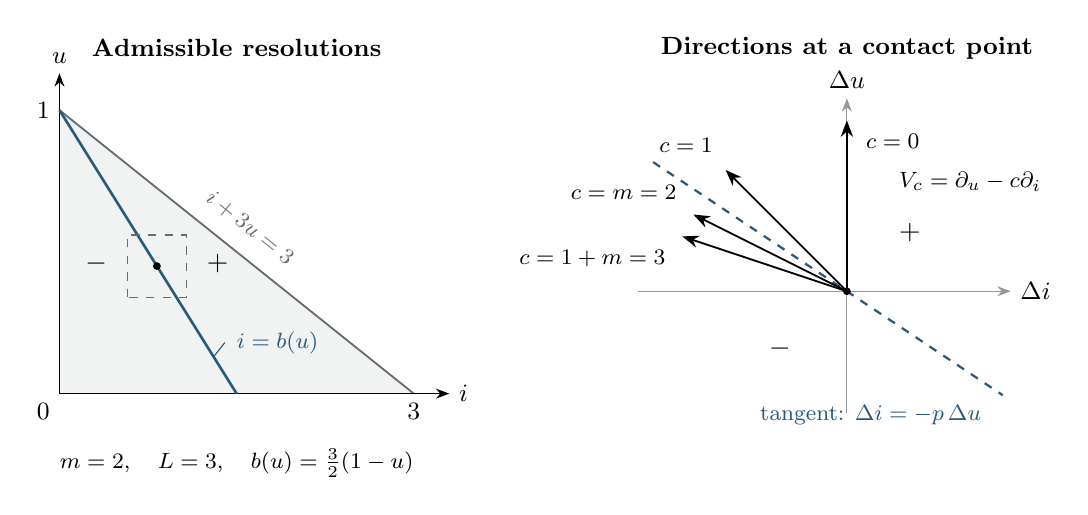
\begin{tikzpicture}[font=\small,>=Stealth,
  direction/.style={->,line width=0.65pt},
  guide/.style={figuregray,dashed,line width=0.5pt}]
  \begin{scope}[x=1.5cm,y=3.6cm]
    \node[font=\small\bfseries] at (1.50,1.22) {Admissible resolutions};
    \fill[figuregray!9] (0,0) -- (3,0) -- (0,1) -- cycle;
    \draw[figuregray,line width=0.65pt] (3,0) -- (0,1)
      node[pos=0.51,above=3pt,sloped,font=\footnotesize] {$i+3u=3$};
    \draw[->] (0,0) -- (3.30,0) node[right] {$i$};
    \draw[->] (0,0) -- (0,1.13) node[above] {$u$};
    \node[below left] at (0,0) {$0$};
    \node[below] at (3,0) {$3$};
    \node[left] at (0,1) {$1$};
    \draw[figureblue,line width=0.95pt] (1.5,0) -- (0,1);
    \node[text=figureblue,anchor=west,font=\footnotesize]
      at (1.42,0.18) {$i=b(u)$};
    \draw[figureblue,line width=0.4pt] (1.40,0.18) -- (1.305,0.13);
    \node[font=\normalsize] at (1.34,0.46) {$+$};
    \node[font=\normalsize] at (0.31,0.46) {$-$};
    \fill (0.825,0.45) circle[radius=1.4pt];
    \draw[guide] (0.575,0.34) rectangle (1.075,0.56);
    \node[anchor=north,font=\footnotesize] at (1.5,-0.16)
      {$m=2,\quad L=3,\quad b(u)=\tfrac32(1-u)$};
  \end{scope}
  \begin{scope}[shift={(10.0,1.30)}]
    \node[font=\small\bfseries] at (0,3.09) {Directions at a contact point};
    \draw[->,figuregray!70] (-2.65,0) -- (2.08,0)
      node[right,text=black] {$\Delta i$};
    \draw[->,figuregray!70] (0,-1.55) -- (0,2.45)
      node[above,text=black] {$\Delta u$};
    \draw[figureblue,dashed,line width=0.8pt]
      (-2.46,1.64) -- (1.98,-1.32);
    \node[text=figureblue,anchor=north east,font=\footnotesize]
      at (1.83,-1.33) {tangent: $\Delta i=-p\,\Delta u$};
    \draw[direction] (0,0) -- (0,2.17);
    \node[anchor=west,font=\footnotesize] at (0.12,1.91) {$c=0$};
    \draw[direction] (0,0) -- (-1.54,1.54);
    \node[anchor=south east,font=\footnotesize] at (-1.58,1.64) {$c=1$};
    \draw[direction] (0,0) -- (-1.95,0.975);
    \node[anchor=south east,font=\footnotesize] at (-2.04,1.04) {$c=m=2$};
    \draw[direction] (0,0) -- (-2.09,0.6967);
    \node[anchor=north east,font=\footnotesize] at (-2.18,0.64) {$c=1+m=3$};
    \fill (0,0) circle[radius=1.4pt];
    \node[font=\normalsize] at (0.80,0.75) {$+$};
    \node[font=\normalsize] at (-0.85,-0.73) {$-$};
    \node[font=\footnotesize,anchor=west] at (0.54,1.39)
      {$V_c=\partial_u-c\partial_i$};
  \end{scope}
\end{tikzpicture}
\caption{The resolution triangle $i\ge0$, $u\ge0$,
$i+(1+m)u\le L$ and the characteristic directions $di/du=-c$,
where $c\in\{0,1,m,1+m\}$.
Each direction $V_c=\partial_u-c\partial_i$ preserves the
corresponding data depth $i+cu$.
The explicit example on the left has $m=2$ and contact slope
$p=-b'(u)=3/2$; its two axes use different drawing scales.
The right panel uses equal scales for the local increments.
The signs mark $\pm(i-b(u))>0$.
At a transverse contact, $p\ne c$, the crossing factor is
$V_c(i-b(u))=p-c$.  Existence of one-sided traces and the associated
jump identities use the hypotheses of Lemma~\ref{lem:curve-traces}.}
\label{fig:characteristic-plane}
\end{figure}


Ambient almost-everywhere differentiability does not solve the local
problem: the entire matched plane lies on the boundary of
\eqref{eq:trace-domain}, and could lie in the ambient exceptional set.
We will obtain the needed traces from the signs of the mixed
derivatives.  Their affine approximation will produce finite entropy
blocks for Section~\ref{sec:rate-transfer}; their measure identities
will later pass those rate constraints to the contact curve.

Here are the properties of $f$ supplied by the finite observations.
It is locally Lipschitz and nondecreasing in every coordinate; its data
derivatives lie between zero and the capacity of that coordinate.  Its
label derivative is nonnegative and locally bounded.  Every mixed
derivative involving two different coordinates, including a data
coordinate and $v$, is a nonpositive distribution in the interior.
We verify the signs, especially the one involving the label.

Advance $v$ to $v'>v$.  Write $a=C_{v'}-C_v$ and
$r=R_{mv}-R_{mv'}$.  Nested labels give
$|a|\lesssim\eps^v$, $|r|\lesssim\eps^{mv}$, and the change of data is
\begin{equation}\label{eq:trace-frame-change}
 X'=X,\quad Y'=Y+aX,\quad W'=W+rX,\quad
 Z'=Z+aW+rY+arX.
\end{equation}
In a data box, the uncertainty in $Y'$ is bounded by a constant times
$\eps^{L_Y}+\eps^{v+L_X}$, and that in $W'$ by a constant times
$\eps^{L_W}+\eps^{mv+L_X}$.  The uncertainty in $Z'$ is bounded by
\[
 C\bigl(\eps^{L_Z}+\eps^{v+L_W}
       +\eps^{mv+L_Y}+\eps^{(1+m)v+L_X}\bigr).
\]
The four inequalities in \eqref{eq:trace-domain} bound these by the
respective target widths.  The inverse shear has the same bounds.
Consequently, conditional on $E_{v'}$, the old and new data descriptions
at fixed admissible depths determine each other with bounded ambiguity.
This assertion also holds at each corner of any coordinate rectangle
contained in the domain.

At fixed labels, a data refinement is determined by the particle and
labels.  Its increase in particle information is therefore exactly its
conditional entropy, up to the bounded bin ambiguities.  A further data
refinement can only decrease this conditional entropy.  For a label
refinement, express both ends of the data refinement in the old frame
conditional on $E_{v'}$, using \eqref{eq:trace-frame-change}.  The two
information increments being compared are then
\[
 \Ent(D_{\rm fine}\mid E_v,D_{\rm coarse})
 \quad\hbox{and}\quad
 \Ent(D_{\rm fine}\mid E_{v'},D_{\rm coarse}),
\]
up to $O(1/\log(1/\eps))$; the latter is no larger than the former.
Here $D_{\rm coarse}$ includes every other data coordinate.  Thus each
mixed rectangle difference of $f_\eps$ is nonpositive up to an error
vanishing as $\eps\downarrow0$.  Passing to the limiting profile proves
the mixed signs, first for rectangle differences and then for
distributions, by integrating the rectangle inequalities against
nonnegative smooth test functions and shrinking the rectangles.

Refining a scalar datum by $d$ costs at most
$d+O(1/\log(1/\eps))$ in normalized entropy; for $U$ the bound is
$2d+O(1/\log(1/\eps))$.  Advancing the labels by $d$ costs at most
$(1+m)d+O(1/\log(1/\eps))$.  The old data are recoverable from the new
observation, and the change of data conditional on the new labels has
bounded ambiguity.  These facts give monotonicity and the asserted
Lipschitz bounds.  For two nearby points on flat faces, move first to a
common slightly finer label so that coordinatewise comparison is
admissible.  This proves the same bounds up to those faces.  The argument
uses vector conditional entropy unchanged when $Y,W$ are grouped.

These comparisons also upgrade the dense diagonal to locally uniform
convergence.  Fix a compact subset $K$ of \eqref{eq:trace-domain} and a
compact relative neighborhood $K^+$ of it.  Uniformly for nearby
$z,z'\in K^+$, the box bounds give
\[
 |f_\eps(z)-f_\eps(z')|
 \le C_K\|z-z'\|_1+O_K(1/\log(1/\eps)).
\]
The same estimate holds at the faces: the common finer label needed
there advances time by $O_K(\|z-z'\|_1)$, and stays in the domain for
nearby points because $K^+$ has label times bounded away from the
endpoints.  For a fixed sufficiently small $\delta>0$, choose a finite
$\delta$-net $z_1,\ldots,z_N$ for $K$ from the dense family in $K^+$.  The same
Lipschitz bound for $f$ then gives
\[
 \sup_{z\in K}|f_\eps(z)-f(z)|
 \le \max_{1\le j\le N}|f_\eps(z_j)-f(z_j)|
       +2C_K\delta+O_K(1/\log(1/\eps)).
\]
First let $\eps\to0$ along the selected sequence, using convergence at
these finitely many net points, and then let $\delta\downarrow0$.
Thus $f_\eps\to f$ locally uniformly on the full closed-sided domain,
including its faces.

\subsection{An abstract trace theorem}

We now isolate the consequence of these mixed signs for a plane whose
data depths move at distinct speeds.  The grouped middle datum at $m=1$
is what makes the speeds distinct in that case.

Let $n\ge2$, let $c_1<\cdots<c_n$ be distinct real numbers, and let
$\mathcal E$ be a nonempty set of ordered pairs $(j,k)$ with $j<k$.
For an open interval $I$ define the closed-sided region
\[
 \mathcal D=\{(\mathbf L,v)\in\RR^n\times I:
       L_k-L_j\le(c_k-c_j)v\text{ for }(j,k)\in\mathcal E\}.
\]
Its interior is obtained by making these inequalities strict.  Define
\begin{equation}\label{eq:trace-plane-cone}
 \begin{split}
 \Pi(i,u)&=(i+c_1u,\ldots,i+c_nu,u),\\
 \mathcal K&=\{\xi\in\RR^{n+1}:
       \xi_k-\xi_j\le(c_k-c_j)\xi_v
                      \text{ for }(j,k)\in\mathcal E\},\\
 V_j&=\partial_u-c_j\partial_i.
 \end{split}
\end{equation}
The cone $\mathcal K$ has nonempty interior and is invariant under
translation by either tangent vector
$e=(1,\ldots,1,0)$ or $t=(c_1,\ldots,c_n,1)$.
In particular, for $h\ge0$, $\Pi(i,u)+h\xi$ belongs to $\mathcal D$ for
$\xi\in\mathcal K$, provided its label time belongs to $I$.

\begin{theorem}[Characteristic-plane traces]\label{thm:characteristic-trace}
Suppose $f$ is locally Lipschitz on $\mathcal D$, and, in its interior,
\[
 0\le f_j\le d_j,\qquad 0\le f_v\le d_v,
 \qquad f_{jk}\le0\ (j\ne k),\qquad f_{jv}\le0
\]
in the distributional sense.  The derivative bounds may instead be local
bounds on each compact neighborhood under consideration; in that
case all conclusions concerning boundedness are local.  Then there
are, up to null sets, uniquely determined locally bounded fields $a_1,\ldots,a_n,D$ on
$\RR\times I$, with $0\le a_j\le d_j$ and $0\le D\le d_v$, having the
following properties.

\begin{enumerate}
\item \emph{Strong traces.} For almost every interior offset $\eta\in\mathcal K^\circ$, the
restrictions of the ambient gradients to $\Pi(\cdot)+\eta$ are defined
almost everywhere.  As $\eta\to0$ through such offsets, they converge
strongly in $L^1_{\rm loc}(di\,du)$ to $(a_1,\ldots,a_n,D)$.
For $Q\Subset Q'\Subset\RR\times I$ this convergence has the bound
\begin{equation}\label{eq:trace-quantitative-slices}
 \|f_\alpha(\Pi(\cdot)+\eta)-A_\alpha\|_{L^1(Q)}
 \le C_Q|\eta|+\omega_{\alpha,Q'}(C_Q|\eta|),
 \qquad A=(a_1,\ldots,a_n,D),
\end{equation}
where $\omega_{\alpha,Q'}(r)\to0$ is the $L^1$ translation modulus of
$A_\alpha$ on $Q'$.  The constant depends only on the local derivative
bounds, the clock speeds, and the two patches.

\item \emph{Measure identities.} There exist locally finite nonnegative measures
$\nu_{jk}=\nu_{kj}$, $j\ne k$, and $\nu_{jv}$ on the plane such that
\begin{equation}\label{eq:trace-mixed-measures}
 V_j a_j=-\nu_{jv}-\sum_{k\ne j}(c_k-c_j)\nu_{jk},
 \qquad \partial_iD=-\sum_j\nu_{jv}.
\end{equation}
For $F=f\circ\Pi$, the weak derivatives are
\begin{equation}\label{eq:trace-plane-derivatives}
 F_i=\sum_j a_j,\qquad F_u=\sum_j c_ja_j+D.
\end{equation}
In particular,
\begin{equation}\label{eq:trace-distribution-inequality}
 V_n a_n\ge\partial_iD
\end{equation}
as measures.  With $q_j=1+c_n-c_j$, the full flux identity is
\begin{equation}\label{eq:trace-measure-flux}
 -\sum_jq_jV_ja_j
 =\sum_{j<k}(c_k-c_j)^2\nu_{jk}+\sum_jq_j\nu_{jv}.
\end{equation}

\item \emph{Affine approximation.} There is a sequence $h_\ell\downarrow0$ and a single null set
$N\subset\RR\times I$ such that, for every $(i,u)\notin N$ and every
finite $R$,
\begin{equation}\label{eq:trace-affine-blowup}
 \lim_{\ell\to\infty}\sup_{\xi\in\mathcal K,\ |\xi|\le R}
 \left|
 \frac{f(\Pi(i,u)+h_\ell\xi)-f(\Pi(i,u))}{h_\ell}
      -\sum_j a_j(i,u)\xi_j-D(i,u)\xi_v
 \right|=0.
\end{equation}
Only sufficiently large $\ell$, for which the displayed label times
belong to $I$, are used.  The sequence may depend on $f$.
\end{enumerate}
\end{theorem}

\begin{proof}
All estimates are local.  Fix nested bounded open plane patches
$Q\Subset Q'\Subset Q''$ and a nonnegative smooth function $\chi$
supported in $Q'$ and equal to one on $Q$.  All small offsets below keep
$\Pi(Q'')+\eta$ in the fixed neighborhood where the derivative bounds
hold.  Smooth $f$ by convolution at a radius smaller than the distance
of the offset patch from the boundary.  The mixed signs and first
 derivative bounds persist.  We first work with this smooth function.

On any parallel interior plane the chain rule gives
\begin{equation}\label{eq:trace-smooth-flux}
 \begin{split}
 \sum_jq_jV_j f_j(\Pi+\eta)
 &=\sum_{j<k}(q_j-q_k)(c_k-c_j)f_{jk}(\Pi+\eta)
       +\sum_jq_jf_{jv}(\Pi+\eta)\\
 &=\sum_{j<k}(c_k-c_j)^2f_{jk}(\Pi+\eta)
       +\sum_jq_jf_{jv}(\Pi+\eta).
 \end{split}
\end{equation}
Let $M$ bound the absolute values of the first derivatives on this
neighborhood.  Multiplication by $-\chi$ and integration by parts gives
\begin{equation}\label{eq:trace-flux-bound}
 \begin{split}
 &\sum_{j<k}(c_k-c_j)^2
    \int\chi(-f_{jk})(\Pi+\eta)
       +\sum_jq_j\int\chi(-f_{jv})(\Pi+\eta)\\
 &\hspace{35mm}\le M\sum_jq_j\|V_j\chi\|_{L^1}.
 \end{split}
\end{equation}
Every integrand on the left is nonnegative.  Since the speeds are
distinct, this controls each mixed derivative separately, uniformly in
the offset and smoothing radius.  For example, the sum of all their
masses on $Q$ is at most
\[
 C_Q=\frac{M\sum_jq_j\|V_j\chi\|_1}
 {\min\{1,\min_{j<k}(c_k-c_j)^2\}}.
\]
Changing $C_Q$ to accommodate larger patches causes no difficulty.

We next construct the strong traces.  Write $\alpha$ for one ambient
coordinate, either a datum or $v$.  Consider interior offsets with
$\eta_\alpha=0$.  Their cone is convex and nonempty: for a data
coordinate $j$ one may take $\eta_v>0$ and all data offsets zero; for
$\alpha=v$ one may take $\eta_k=-c_k$ and $\eta_v=0$.
If $\eta_\alpha=\eta'_\alpha=0$, the fundamental theorem of calculus
along their segment, followed by \eqref{eq:trace-flux-bound}, gives
\begin{equation}\label{eq:trace-own-coordinate}
 \begin{split}
 &\|f_\alpha(\Pi+\eta)-f_\alpha(\Pi+\eta')\|_{L^1(Q)}\\
 &\quad\le\sum_{\beta\ne\alpha}|\eta_\beta-\eta'_\beta|
       \int_0^1\int_Q
       |f_{\alpha\beta}(\Pi+(1-s)\eta+s\eta')|\,di\,du\,ds
 \le C_Q|\eta-\eta'|.
 \end{split}
\end{equation}
Only mixed derivatives occur in this estimate.

For completeness, this slice estimate passes to the nonsmooth function
without choosing an arbitrary restriction of an $L^\infty$ field.  On
compact interior sets the smoothed gradients converge to the weak
gradients in $L^1$.  The linear map
\[
 (i,u,\eta)\longmapsto\Pi(i,u)+\eta,
 \qquad \eta_\alpha=0,
\]
has full rank.  Fubini's theorem and a subsequence therefore give
$L^1(Q)$ convergence of the smoothed restrictions for almost every such
offset.  Exhaust the allowable offset sets and patches countably.  For
any two offsets in the resulting full-measure set, their compact
connecting segment is interior, so \eqref{eq:trace-own-coordinate}
passes to the limit.  It makes the restrictions an $L^1(Q)$ Cauchy family
as their offsets tend to zero.  The limits on different patches agree;
call the resulting field $A_\alpha$.  Letting $\eta'\to0$ gives
\[
 \|f_\alpha(\Pi+\eta)-A_\alpha\|_{L^1(Q)}\le C_Q|\eta|
 \quad\text{when }\eta_\alpha=0.
\]
The derivative bounds pass to this limit.

For a general data offset remove its $j$th component by replacing
$\eta$ with $\eta-\eta_je$ and translating $i$ by $\eta_j$.
For the label derivative replace $\eta$ with $\eta-\eta_vt$ and
translate $u$ by $\eta_v$.  Cone membership is unchanged by these
operations.  Translation continuity in $L^1$ now proves
\eqref{eq:trace-quantitative-slices}, for almost every general offset.
It also proves uniqueness of the traces.  No pointwise modulus of
continuity of the gradients has been used.

Choose interior offsets tending to zero for which all the gradient
restrictions converge strongly on the countable exhaustion of patches.
For each offset choose a still smaller convolution radius so that the
smoothed restrictions have the same limits.  The nonnegative measures
on each slice with densities $-f_{jk}$ and $-f_{jv}$ have locally bounded
masses by \eqref{eq:trace-flux-bound}.  Successive weak measure limits,
with a diagonal choice on the patches, give $\nu_{jk}$ and $\nu_{jv}$.
The slice identities
\[
 V_jf_j=f_{jv}+\sum_{k\ne j}(c_k-c_j)f_{jk},
 \qquad \partial_if_v=\sum_jf_{jv}
\]
pass to the limit against smooth test functions, proving
\eqref{eq:trace-mixed-measures} and \eqref{eq:trace-measure-flux}.
The potentials on these slices converge locally uniformly to $F$,
whereas their tangential derivatives converge strongly in $L^1$.
This gives \eqref{eq:trace-plane-derivatives}.  Finally,
\[
 V_na_n-\partial_iD
 =\sum_{k<n}(c_n-c_k)\nu_{nk}+\sum_{j<n}\nu_{jv}\ge0,
\]
which proves \eqref{eq:trace-distribution-inequality}.
The measures used to represent the mixed derivatives need not be
unique; the trace fields and the distributional conclusions are unique.

It remains to prove the assertion about this particular plane.
For a bounded base patch $Q$ and an integer $R\ge1$, define
\[
 e_{h,Q,R}(i,u)=\int_{\mathcal K\cap B_R}
       |\nabla f(\Pi(i,u)+h\xi)-A(i,u)|\,d\xi.
\]
The boundary of the cone has ambient measure zero and is irrelevant to
this integral.  The strong slice convergence, Fubini's theorem and the
boundedness of the gradients show that
\begin{equation}\label{eq:trace-integrated-gradient}
 \int_Qe_{h,Q,R}\longrightarrow0\qquad(h\downarrow0).
\end{equation}
More quantitatively the integral is bounded by a constant depending on
$R,Q$ times $h+\sum_\alpha\omega_{\alpha,Q'}(C_Rh)$.
Choose $h_\ell\downarrow0$ so that the integrals in
\eqref{eq:trace-integrated-gradient} are at most $2^{-\ell}$ for the
first $\ell$ members of a countable exhaustion of patches and radii.
The summability of these integrals implies
$e_{h_\ell,Q,R}(i,u)\to0$ outside one null set.

Fix a point outside that set.  The rescaled potentials
\[
 g_\ell(\xi)=
 \frac{f(\Pi(i,u)+h_\ell\xi)-f(\Pi(i,u))}{h_\ell}
\]
are uniformly Lipschitz on each bounded part of $\mathcal K$ and vanish
at zero.  Every locally uniformly convergent subsequence has weak
gradient equal to the constant $A(i,u)$ in $\mathcal K^\circ$, by the
mean gradient convergence just proved.  This interior is connected.
Thus the limit is $A(i,u)\cdot\xi$ there, and continuity gives the same
identity on the closed cone, including its vertex and faces.
Compactness of the uniformly Lipschitz functions and uniqueness of
this limit imply convergence of the whole chosen sequence, as stated
in \eqref{eq:trace-affine-blowup}.
\end{proof}

\subsection{Finite approximation after selecting the block scale}

The next consequence specifies exactly what is required of the finite
entropy systems.  Its exceptional set is a set of base points on the
plane; probabilistic trimming of conditional cells is a separate use
of Lemma~\ref{lem:homogenization} and
Theorem~\ref{thm:finite-conditioning}.

\begin{corollary}[Quantified finite profile approximation]
\label{cor:finite-characteristic-trace}
Assume Theorem~\ref{thm:characteristic-trace}, and let $f_\eps\to f$
locally uniformly on $\mathcal D$ along the sequence of finite systems
under consideration.  Fix a bounded measurable base patch $Q$ of
positive measure with compact closure in $\RR\times I$, a radius
$R\ge1$, an error $\eta>0$, an exceptional proportion $0<\tau<1$,
and a maximum block length $h_*>0$.  There exist
\[
 0<h<h_*,\qquad G\subset Q,\qquad |Q\setminus G|\le\tau|Q|,
\]
and a compact neighborhood $K_0\subset\mathcal D$ containing all
$\Pi(q)+h\xi$ with $q\in\overline Q$, $\xi\in\mathcal K\cap B_R$,
such that the following holds.  If
\begin{equation}\label{eq:trace-finite-tolerance}
 \|f_\eps-f\|_{L^\infty(K_0)}\le\eta h/4,
\end{equation}
then, simultaneously for every $q\in G$ and every
$\xi\in\mathcal K\cap B_R$,
\begin{equation}\label{eq:trace-finite-affine}
 |f_\eps(\Pi(q)+h\xi)-f_\eps(\Pi(q))-hA(q)\cdot\xi|
 \le\eta h.
\end{equation}
In particular, for every finite family of such displacements, every
information increment between two of them differs from its affine
value by at most $2\eta h$.  An alternating sum of $r$ profile values
whose affine contributions cancel has absolute value at most
$r\eta h$.

All dependencies have the order
\[
 f,\ Q,R,\eta,\tau,h_*\quad\longrightarrow\quad h,G,K_0
 \quad\longrightarrow\quad\eps_0.
\]
For every member of the converging finite sequence with
$\eps<\eps_0$, \eqref{eq:trace-finite-tolerance} holds.  If finitely many
entropy identities also incur a total normalized ambiguity error at
most $B/\log(1/\eps)$, one may, after choosing $h$, require in addition
\[
 \log(1/\eps)\ge B/(\eta h).
\]
Each such combined identity then has at most one additional $\eta h$
of error.  More generally one may prescribe any sequences
$\eta_\ell,\tau_\ell\downarrow0$ and $h_{*,\ell}\downarrow0$ and
select successively $h_\ell<h_{*,\ell}$, then the inner approximation
thresholds.  If $\sum_\ell\tau_\ell<\infty$, almost every point of $Q$
belongs to all but finitely many of the resulting $G_\ell$.
\end{corollary}

\begin{proof}
On $Q$, the supremum error in \eqref{eq:trace-affine-blowup} tends to
zero almost everywhere along the chosen sequence and is uniformly
bounded by the Lipschitz bounds times $R$.  Choose a term $h<h_*$
small enough that the subset on which this error exceeds $\eta/2$
has measure at most $\tau|Q|$, and that all shifted label times stay
inside $I$.  Its complement is $G$.  A compact neighborhood $K_0$
exists because $Q$ and the displacement set are bounded.  The two
profile approximation errors in the difference in
\eqref{eq:trace-finite-affine} total at most $\eta h/2$, proving that
inequality.  Subtracting increments, or summing the individual errors,
gives the finite-family assertions.  Uniform convergence supplies
$\eps_0$ after $h$ has been fixed.  The ambiguity condition and the
last exceptional-set assertion follow respectively by addition of
errors and summability of the measures of $Q\setminus G_\ell$.
\end{proof}

There is no uniform choice of $h$ for all Lipschitz profiles in this
corollary.  The translation moduli in
\eqref{eq:trace-quantitative-slices}, and hence the block scale, depend
on the limiting profile.  At a fixed nonexceptional plane point one
may equivalently use its sequence in
\eqref{eq:trace-affine-blowup}, choose a block from that sequence, and
then make the finite-system errors small compared with that block.

For the profile \eqref{eq:trace-domain}, the clocks are
$c_X=0,c_Y=1,c_W=m,c_Z=1+m$, ordered increasingly when applying the
theorem.  Write the trace fields as $x,y,w,z,D$.  At $m=1$ the clocks
are $0,1,2$, the fields are $x,q,z,D$, and $q=a_U$; notation such as
$y+w$ means $q$ and asserts no separate traces for $Y,W$.
Thus \eqref{eq:trace-distribution-inequality} reads
\begin{equation}\label{eq:trace-z-D}
 (\partial_u-(1+m)\partial_i)z\ge\partial_iD.
\end{equation}
The distinction between grouped and separate depths is necessary:
$f(L_Y,L_W)=\max(L_Y,L_W)$ has nonpositive mixed derivatives, but its
separate first derivatives have different traces from the two sides
of $L_Y=L_W$.  On the grouped domain it is simply $f(L_U)=L_U$.

\subsection{Traces on a contact curve}

We need a second trace statement within the plane.  It uses bounded
variation in one direction at a time; it does not require the entire
gradient of each rate field to be a measure.

\begin{lemma}[Transverse traces on a Lipschitz curve]
\label{lem:curve-traces}
Let $b$ be Lipschitz on an interval $J$, and let
$\Gamma=\{(b(u),u):u\in J\}$ lie in an open plane region.
Suppose bounded fields $a_j,D$ in this region satisfy
$V_ja_j\in\mathcal M_{\rm loc}$ and
$\partial_iD\in\mathcal M_{\rm loc}$, where $\mathcal M_{\rm loc}$
denotes locally finite signed measures. Put~$p(u)=-b'(u)$ at points
where this derivative exists.  For almost every $u\in J$ the field
$D$ has two strong traces $D^-,D^+$ and every $a_j$ with
$c_j\ne p(u)$ has two strong traces $a_j^-,a_j^+$.  Specifically, at
$q_0=(b(u_0),u_0)$ the mean of
$|a_j-a_j^\pm(u_0)|$ tends to zero on the corresponding tangent
half-ball
\[
 B_\rho(q_0)\cap
 \{\ \pm(i-b(u_0)+p(u_0)(u-u_0))>0\ \},
 \qquad\rho\downarrow0,
\]
and likewise for $D$.  The same assertion holds with the actual
sides $\pm(i-b(u))>0$.  No assertion is made about the field whose
speed equals $p(u_0)$.

If, in addition, $V_na_n\ge\partial_iD$, then at almost every
transverse point $p\ne c_n$,
\begin{equation}\label{eq:trace-curve-jump}
 D^- -D^+\ge(c_n-p)(a_n^+-a_n^-).
\end{equation}
These conclusions apply to curves on the boundary of an aperture
region whenever the fields are defined in an ambient neighborhood;
one then retains only the side lying in that region.
\end{lemma}

\begin{proof}
We first justify the one-direction slicing fact being used.  If
$g\in L^\infty$ on a rectangle with coordinates $(s,r)$ and
$\partial_sg$ is a finite measure, then for almost every $r$ the
one-dimensional function $g_r(s)=g(s,r)$ has bounded variation, and
its derivative measures satisfy, on smaller rectangles,
\begin{equation}\label{eq:trace-slicing}
 \partial_sg=\int Dg_r\,dr,
 \qquad |\partial_sg|=\int |Dg_r|\,dr.
\end{equation}
Here integration of measures means integration of their values
against compactly supported continuous test functions.  To verify
this, convolve $g$ in the rectangle.  The integrals of
$|\partial_sg_\varrho|$ on a smaller rectangle are bounded by the
variation of $\partial_sg$ on a slightly larger one.  Choose a
subsequence with $g_\varrho(\cdot,r)\to g(\cdot,r)$ in $L^1(ds)$ for
almost every $r$.  The definition of one-dimensional variation as
the supremum over finite partitions, or over test functions bounded
by one, and Fatou's lemma give integrable variations of the slices.
Fubini and one-dimensional integration by parts then identify
$\partial_sg$ with $\int Dg_r\,dr$.  The variation equality follows
by taking the supremum over a countable dense family of scalar test
functions on rational subintervals, selecting these tests measurably
in $r$, and approximating the resulting bounded tests by continuous
ones.  Exhaustion gives \eqref{eq:trace-slicing} locally.

Suppose first the curve is a Lipschitz graph $s=h(r)$ in these
coordinates.  The one-dimensional representatives have limits
$T^\pm(r)=g_r(h(r)\pm)$ for almost every $r$.  Fix a compact graph
patch and define
\[
 q_\varrho(r)=|Dg_r|\bigl((h(r)-\varrho,h(r)+\varrho)
                                      \setminus\{h(r)\}\bigr).
\]
For small fixed $\varrho$, these functions are integrable by
\eqref{eq:trace-slicing}, and they decrease to zero almost everywhere
as $\varrho\downarrow0$.  Outside one null set we may assume that
$r_0$ is a Lebesgue point of $T^+,T^-$ and of every $q_{1/k}$ for
which the graph patch permits that collar.  If
$|r-r_0|<C\rho$ and $0<\pm(s-h(r))<C\rho$, then
\[
 |g(s,r)-T^\pm(r_0)|
 \le q_{C\rho}(r)+|T^\pm(r)-T^\pm(r_0)|
\]
for almost every $(s,r)$.  Integrating in such a graph-side cylinder
and dividing by $\rho^2$ bounds the result by
\[
 \frac{C}{\rho}\int_{|r-r_0|<C\rho}
       \bigl(q_{C\rho}(r)+|T^\pm(r)-T^\pm(r_0)|\bigr)\,dr.
\]
For each fixed $k$, eventually $q_{C\rho}\le q_{1/k}$.
Lebesgue differentiation first, then $k\to\infty$, shows that this
bound tends to zero.  At a point where $h$ is differentiable, the
area between its graph and its tangent in a radius-$\rho$ disk is
$o(\rho^2)$.  Boundedness of $g$ therefore gives the same strong mean
traces on tangent half-disks.  Invertible linear changes of coordinates
preserve this conclusion for half-balls, because the corresponding
ellipses contain and are contained in comparable balls.

For $a_j$ use the coordinates
\[
 s=u,\qquad r=i+c_ju,
\]
so that $V_j=\partial_s$ and the curve has projection
$r=g_j(u)=b(u)+c_ju$.  On the set where $g_j'=c_j-p\ne0$ this
projection can be covered, apart from a null set, by countably many
sets on each of which it is bi-Lipschitz.  Here is a direct reason.
At a differentiability point with $g_j'\ne0$, choose integers $k,N$
so that $|g_j'|>2/k$ and
\[
 |g_j(v)-g_j(u)-g_j'(u)(v-u)|\le |v-u|/k
 \quad\text{if }|v-u|<1/N.
\]
Partition these points according to $k,N$, the sign of the derivative,
and intervals of length less than $1/N$.  Any two points of one piece
then have image distance at least $|v-u|/k$; the upper Lipschitz bound
is inherited from $g_j$.  On each image piece the inverse extends
to a Lipschitz function $h(r)$ on an interval.  The graph argument
above applies to this extension.  At almost every density point of
the original piece its tangent is the original tangent.  The
bi-Lipschitz parameter change takes exceptional null sets back to
null sets.  This proves the traces for $a_j$ on its transverse set.
For $D$, simply take $s=i,r=u$, so the curve is already the graph
$s=b(r)$ and is everywhere transverse.  Taking the union of the
finitely many exceptional sets proves the simultaneous assertion.
The area comparison also replaces tangent sides by actual sides.

Finally, \eqref{eq:trace-slicing} identifies the part of the derivative
measure on $s=h(r)$ as $(T^+(r)-T^-(r))\,dr$, since a
one-dimensional BV derivative has an atom equal to its jump.
On each transverse inverse patch, substitute
$dr=|c_j-p(u)|\,du$.  The positive $s$ side is the positive $i-b(u)$
side precisely when $p-c_j>0$, so reversing the sides when necessary
gives the signed factor $p-c_j$.  Partition the countable patches
into disjoint measurable pieces before summing.  There is no omitted
measure on a parameter-null subset of the curve: its projection under
the Lipschitz map $g_j$ is null, and \eqref{eq:trace-slicing} gives zero
variation over such a projection.  In the original $(i,u)$ coordinates
we have therefore proved
\begin{equation}\label{eq:trace-graph-measures}
 (V_ja_j)|_\Gamma
   =(p-c_j)(a_j^+-a_j^-)\,du,
 \qquad
 (\partial_iD)|_\Gamma=(D^+-D^-)\,du
\end{equation}
on the transverse part of the parameter set.  To check the first
sign and factor directly, set $\varphi(i,u)=i-b(u)$.  Then
$V_j\varphi=p-c_j$, and differentiating a function with jump
$a_j^+-a_j^-$ across $\varphi=0$ gives exactly that factor times
$\delta(\varphi)\,di\,du=(du)|_\Gamma$.
This agrees with the change of variable in the sliced jump measures,
so it applies to the bounded fields just considered.  Restrict the
nonnegative measure $V_na_n-\partial_iD$ to the transverse part of
$\Gamma$ and use
\eqref{eq:trace-graph-measures}; its nonnegative density is
\[
 (p-c_n)(a_n^+-a_n^-)-(D^+-D^-).
\]
This is precisely \eqref{eq:trace-curve-jump}.  An aperture boundary
requires no further trace argument: all statements were proved in
the ambient plane neighborhood before a side is selected.
\end{proof}

\section{Rate transfer at matched clocks}
\label{sec:rate-transfer}

We keep the saturated homogeneous component $p_\eps$ selected in
Section~\ref{sec:characteristic-plane}, with least aspect $m>0$.
Its information and time profiles are $f,S$, and its matched-plane
potential is $\Phi=f\circ\Pi_m$ from
\eqref{eq:matched-plane-profile}.  The row data and their admissible
depths are those of \eqref{eq:trace-variables} and
\eqref{eq:trace-domain}.  Write $x,y,w,z$ for their plane trace rates
and $D$ for the label rate.  When $m=1$, the middle datum is
$U=(Y,W)$ and its single rate is $q=a_U$.  The matched component
defining $f,S,\Phi$ is fixed before their trace points.  Later
homogeneous selections concern the derived block laws and do not
redefine these profiles.

\begin{proposition}[Matched-clock rate transfer]
\label{prop:rate-transfer}
For almost every point $(i,u)$ of the characteristic plane with $i>0$
and $0<u<1$, put $s=S'(u)$.  There is a constant $\sigma>0$,
depending only on the matched process and $m$, for which $0<s\le1$
and the following assertions hold.
\begin{enumerate}
\item If $m\ne1$, each of the chains $x\longrightarrow y$ and
$w\longrightarrow z$ has the rule
\[
 d>0\quad\Longrightarrow\quad e\ge\min(1,d+s),
\]
where $d,e$ are its source and target rates.  Each of
$x\longrightarrow w$ and $y\longrightarrow z$ has the same rule
with $\sigma$ in place of $s$.
\item If $m=1$, then
\[
 x>0\Longrightarrow q\ge s,\qquad
 x>0,\ z<1\Longrightarrow z\ge x+s,\qquad
 z<1\Longrightarrow q\le2-s.
\]
\end{enumerate}
The bounds include $0\le x,y,w,z\le1$, or $0\le q\le2$ in
the tied case, supplied by the coordinate capacities.
\end{proposition}

The proof first extracts a finite point--parameter law from an
affine entropy block.  That law will carry the parameter
nonconcentration, coordinate support counts, and product comparisons
used by the projection tests.  Distinct clocks give the four
rate transfers directly.  At tied clocks, the joint rate $q$ is
supplemented by directions between parameter samples and two
conditional projection tests.

\subsection{The selected profiles and the parameter children}

We first verify what the already selected sequence $p_\eps$ supplies
at the depths needed here.  Its initial homogeneous list contains all
finite tuples from a countable dense family of admissible configurations,
including the indicated conditional probabilities given $T$.
For two nearby configurations, give both descriptions the finer label
clock.  The box comparisons in Section~\ref{sec:characteristic-plane}
give bounded ambiguity for changing the data frame at a fixed admissible
resolution.  A depth change of size $a$ introduces at most
$\eps^{-Ca+o(1)}$ possibilities, also conditional on $T$, on each fixed
compact depth range.  Applying the conditional-surprise counting bound
from Lemma~\ref{lem:profile-diagonal} to both descriptions extends the
homogeneous exponents from the dense family to every fixed admissible
configuration.  The same argument applies to finite tuples.  It does
not require independent data refinements to remain admissible at the
coarse label clock.

Write $\mathfrak h(A)$ for the limiting normalized entropy of a listed
observation.  For a finite pair $A,B$, the selected homogeneous
probabilities give, in probability,
\begin{equation}
 -\logeps{p_\eps(B\mid A)}
 =\mathfrak h(A,B)-\mathfrak h(A)+o(1).
 \label{eq:rate-ratio}
\end{equation}
The same statement holds for listed probabilities conditional on $T$;
the probability of $T$ itself is never binned.  After a trace point,
a positive block length $h$, and a finite list of real configurations
have been chosen, take one event $\mathcal E_\eps$ on which all their original
conditional surprises differ from their limiting exponents by at most
$\omega_\eps=o(h)$.  Its probability tends to one.  On this event,
ratios of the joint and parent masses give uniform upper conditional
masses and upper retained support counts.  The support count follows
by dividing the upper mass of a parent by the lower mass of each
retained joint value.

This finite real-depth event is imposed before any restriction which
uses its bounds.  If a later law satisfies
$\mathsf Q\le Kp_\eps(\,\cdot\mid\mathcal E_\eps)$, with
$\log K=o(h\ell)$ and $\ell=\log(1/\eps)$, its conditional entropy
of each listed child given its listed parent differs from the listed exponent by
at most $\omega_\eps+\log(K/p_\eps(\mathcal E_\eps))/\ell$, by
conditional relative entropy and the support count.  The parent
likelihood and child-support thresholds in the proof of
Lemma~\ref{lem:homogenization} give the same absolute error bound for
realized surprise, with $\log(1/\eta)/\ell$ added, outside
$\mathsf Q$-mass at most $2\eta$; choose $\eta\downarrow0$ with
$\log(1/\eta)=o(h\ell)$.  The dense-list
profiles remain the same under this high-probability restriction by
Lemma~\ref{lem:profile-diagonal}.  This verifies the finite inheritance
for the component selected in Section~\ref{sec:characteristic-plane};
it does not select a new $f$ or assert uniform bins at all real depths.

For this component the prediction identities and the positive constant
obtained from its least-aspect argument are
\begin{equation}
 \Ent(R_{mv}\mid T,C_v)=0,\qquad
 \Ent(R_{m(v+a)}\mid T,C_v)\ge\kappa a
 \quad(0<v<v+a<1).
 \label{eq:rate-prediction}
\end{equation}
These are limiting normalized statements for this same $p_\eps$.

Fix a regular plane point $(i,u)$ and a trace block length $h>0$.
Write $E$ for the coarse observation at $\Pi_m(i,u)$ and put
$\rho=\eps^h$.  Given the coarse label, $E$ is a function of
$(T,C_u,R_{mu})$ up to bounded grid choices, which we record when
needed.  Choose $K>\max(1,1/m)$, fixed throughout this construction,
and define the normalized parameter increments
\[
 c=\eps^{-u}(C_{u+Kh}-C_u),\qquad
 r=-\eps^{-mu}(R_{m(u+Kh)}-R_{mu}).
\]
The full finite label $\theta$ records the advanced label and the
bounded choices just mentioned.  Before all tests, fix one half-open
dyadic tree on a fixed bounded box containing the normalized pair
$(c,r)$.  For every real $0\le d\le1$, let $\Theta_d$ be its atom at
level
\[
 n_\rho(d)=\left\lceil d\log_2(1/\rho)\right\rceil.
\]
These atoms are exactly nested for all real depths: $\Theta_a$ is
determined by $\Theta_b$ when $a\le b$, and each $\Theta_a$ atom has
at most
\[
 4^{n_\rho(b)-n_\rho(a)}\le4\rho^{-2(b-a)}
\]
$\Theta_b$ children.  The time prefix records $C_{u+dh}$ and the
normal prefix records $R_{mu+dh}$ up to bounded ambiguity over $E$.
For other finite observations whose nesting holds only up to bounded
choices, we append the parent to the child when needed.  Here $h$ and
the finite prefix list are fixed before $\eps\to0$.

The chain rule gives
\begin{align}
 \Ent(C_{u+dh}\mid E)
 &\ge\Ent(C_{u+dh}\mid T,E)\notag\\
 &\ge S(u+dh)-S(u)-\Ent(R_{mu}\mid T,C_u)-o(1),
 \label{eq:rate-time-child}\\
 \Ent(R_{mu+dh}\mid E)
 &\ge\Ent(R_{mu+dh}\mid T,C_u,R_{mu})-o(1)\notag\\
 &\ge(\kappa/m)dh-o(1).
 \label{eq:rate-normal-child}
\end{align}
For the first inequality, the data in $E$ are determined by the
particle and coarse labels, and adjoining $R_{mu}$ costs at most its
conditional entropy.  The second uses
\eqref{eq:rate-prediction} at time increment $dh/m$.
Prediction also gives
\[
 \kappa a\le\Ent(R_{m(u+a)}\mid T,C_u)
       \le S(u+a)-S(u)+o(1).
\]
Consequently $s=S'(u)\ge\kappa>0$ at the regular points used below.
Fix any $0<\sigma<\min(1,\kappa/m)$.

At tied clocks there is also a bound between any two tested parameter
prefixes.  If $m=1$ and $0\le a<b\le1$, then conditional on $E$ the
symbol $\Theta_a$ is equivalent to
$(C_{u+ah},R_{u+ah})$ up to the recorded bounded choices.  Therefore
\begin{align}
 \Ent(\Theta_b\mid E,\Theta_a)
 &\ge\Ent(C_{u+bh}\mid T,E,\Theta_a)\notag\\
 &\ge S(u+bh)-S(u+ah)
       -\Ent(R_{u+ah}\mid T,C_{u+ah})-o(1)\notag\\
 &=S(u+bh)-S(u+ah)-o(1).
 \label{eq:rate-joint-child-entropy}
\end{align}
After $T,C_{u+ah}$ have been given, the extra conditioning in
$E,\Theta_a$ is a function of $R_{u+ah}$ and the bounded choices.
This is the stated entropy cost and does not use an entropy bound for $T$.

The homogeneous joint symbols $(E,\Theta_a)$ and $(E,\Theta_b)$
turn this last entropy inequality into a bound on their probability
ratio.  On the common real-depth event,
\begin{equation}
 p_\eps(\Theta_b\mid E,\Theta_a)
 \le\eps^{S(u+bh)-S(u+ah)-o(1)}
 \quad(m=1)
 \label{eq:rate-joint-child-mass}
\end{equation}
at every retained child.  The time and normal inequalities give the
corresponding marginal prefix bounds by the same ratio calculation.
Lemma~\ref{lem:typical-conditioning}, with the coarse observation
as $C$ and each listed parent containing $C$, selects base cells
of adequate relative retention without an inverse original cell mass.
We will keep the event as an unnormalized allowed set inside the
chosen base cell until both product comparisons have been imposed.

\subsection{One finite affine-block law}

Center the common pre-label data in the boxes of $E$, dilate them
to bounded coordinates, and round the resulting point $P$ at
precision $\rho$.  For a full label with normalized increment
$(c,r)$ define its canonical post-coordinate symbols by applying
the shear to this same rounded point and then taking the indicated
grid bins:
\begin{equation}
 X_\theta=X,\qquad Y_\theta=Y+cX,\qquad
 W_\theta=W+rX,\qquad
 Z_\theta=Z+cW+rY+crX.
 \label{eq:rate-shear}
\end{equation}
The same origin is transformed at every label, so the shears compose
by adding $(c,r)$ and the map from frame $0$ to frame $1$ uses
$\theta_1-\theta_0$.  Applying the shear before or after rounding
changes each real output by $O(\rho)$.  The canonical bins and the
physically recorded bins consequently determine one another with
bounded conditional ambiguity.  We use the canonical symbols in
the finite law below: each is a genuine function of $(P,\theta)$.
Their prefixes and joint numerator and denominator symbols are
included in the finite uniformization list.  Bounded ambiguity
transfers the entropy identities to these symbols; their own
uniform probability bins, rather than a pointwise assertion from
that ambiguity alone, will supply the retained mass bounds.

Let $\mathcal I=\{X,Y,W,Z\}$ when $m\ne1$, and
$\mathcal I=\{X,U,Z\}$ when $m=1$, with $U=(Y,W)$.
Write $Q_{j,\theta}$ for the canonical coordinate in group
$j\in\mathcal I$, and $(Q_{j,\theta})_d$ for its prefix at precision
$\rho^d$.  Put $(a_X,a_Y,a_W,a_Z)=(x,y,w,z)$ in the distinct-clock
case and $(a_X,a_U,a_Z)=(x,q,z)$ in the tied case.
Choose the fixed $K$ large enough that raising any
individual data depth by at most $h$ is admissible after the label
advances by $Kh$.  For any fixed finite list of $t_j\in[0,1]$, the
affine trace gives
\begin{equation}
 \Ent\bigl(((Q_{j,\theta})_{t_j})_{j\in\mathcal I}
          \mid E,\theta\bigr)
 =h\sum_{j\in\mathcal I} a_jt_j+o(h).
 \label{eq:rate-post-affine}
\end{equation}
Indeed, at the advanced label the unrefined pre- and post-data
determine one another to bounded ambiguity by
\eqref{eq:trace-domain}.  The difference between the information
with the selected refinements and this common base information is
their conditional entropy, because the particle and label determine
the refinement.  The affine trace gives the displayed increment,
and the canonical rounding costs only bounded ambiguity.

Raising all data depths by $h$ is also admissible at the original
label and is preserved under the label-conditioned shear.  The same
calculation gives
\begin{equation}
 \Ent(P\mid E)=h\sum_j a_j+o(h),\qquad
 \Ent(P\mid E,\theta)=h\sum_j a_j+o(h),\qquad
 \Mut(P;\theta\mid E)=o(h).
 \label{eq:rate-pre-independence}
\end{equation}
In particular, the conditional coordinate multiinformation obtained
by subtracting the joint entropy in \eqref{eq:rate-post-affine}
from the sum of its single-coordinate entropies is $o(h)$.
Both information quantities are nonnegative averages over the base
observation $E$.

We now form one sequence of finite blocks.  This order is needed
because the trace error divided by a fixed $h$ need not vanish as
only $\eps$ tends to zero.  Choose $h_n\downarrow0$ on the trace
subsequence for this fixed profile and plane point, so that its
affine error divided by $h_n$ tends to zero uniformly on the bounded
cone of displacements just used.  Differentiability of $S$ gives
the analogous convergence for its time increments.  At stage $n$,
include the first $n$ tuples from a countable list of rational block
prefixes, their canonical joint numerator and denominator symbols,
and the finitely many information differences above.  These are
real original depths fixed by the already chosen $h_n$.

Choose $\eps_n$ within the converging sequence $p_\eps$ so that all
finite probability, prediction, information, and box-ambiguity
errors are at most $\eta_n h_n$, where $\eta_n\downarrow0$, and
$h_n\log(1/\eps_n)\ge n$.  Put
\[
 \rho_n=\eps_n^{h_n},\qquad L_n=\log(1/\rho_n).
\]
For this extraction, let $\mathcal H_n$ contain only the tested
prefix conditions whose truth, after $E$ is fixed, is determined
by the canonical pair $(P,\theta)$: the parameter prefixes and
canonical coordinate numerator and denominator symbols.  The earlier
bins conditional on $T$ need not be pair-measurable.  They are used
to justify the entropy estimates, but are not included in
$\mathcal H_n$.
The two nonnegative information quantities and the failure
probability of the common prefix event can be selected
simultaneously on the base cells by Markov's inequality.  Choose
deterministic $d_n,\zeta_n,\omega_n\downarrow0$ so that, on every
selected base cell, the two natural-log quantities are at most
$d_nL_n$, the prefix event fails with probability at most $\zeta_n$,
and its normalized surprise errors are at most $\omega_n$ in block
units.  The finite lists and thresholds are chosen before the
precision; increasing them slowly gives these common envelopes.
Select one such cell $E=e_n$ and let $p_n^0$ be the original
conditional law of the canonical pair $(P,\theta)$ on that cell,
before normalizing the prefix event $\mathcal H_n$.  Thus
$p_n^0(\mathcal H_n)\ge1-\zeta_n$.  The cell may have small original
mass: the selected bounds are bounds for its conditional law and
contain no inverse mass of $E=e_n$.

For clarity, the two comparisons to be imposed on this law have
different spaces and factors.  Put
\[
 \mu_n^0=(p_n^0)_P,\qquad
 \lambda_n^0=(p_n^0)_\theta,\qquad
 \xi_{j,n}^{0,\theta}=(p_n^0)_{Q_{j,\theta}\mid\theta}.
\]
The first comparison is with
$\mu_n^0(P)\lambda_n^0(\theta)$.  The second is with
\[
 \lambda_n^0(\theta)
       \prod_{j\in\mathcal I}\xi_{j,n}^{0,\theta}(Q_{j,\theta});
\]
it uses the coordinate factors conditional on that label.
The divergences from these two probability laws are respectively
the pair information and the averaged conditional coordinate
multiinformation, each bounded by $d_nL_n$.  We do not assume a
uniform multiinformation estimate on individual labels.


\begin{lemma}[A finite core for a point--parameter law and its coordinates]
\label{lem:affine-block-core}
Fix an integer $k\ge1$.  Let $p^0$ be a probability law on a finite pair space
$\mathcal P\times\Theta$.  Write $\mu^0=p^0_P$ and
$\lambda^0=p^0_\theta$.  Let
$Q_j=Q_j(P,\theta)$, $1\le j\le k$, be finite coordinate
observations, and put
$\xi_j^\theta=p^0_{Q_j\mid\theta}$ on positive label fibers, choosing
an arbitrary probability law on a zero-mass label fiber.
Define the two nonnegative natural-log quantities
\begin{align*}
 D_{\mathrm{pair}}
 &=\KL(p^0_{P,\theta}\Vert\mu^0\otimes\lambda^0),\\
 D_{\mathrm{coord}}
 &=\KL\left(p^0_{\theta,Q_1,\ldots,Q_k}
       \middle\Vert
       \lambda^0(\theta)\prod_{j=1}^k\xi_j^\theta(Q_j)\right)\\
 &=\sum_{j=1}^k\Entn^{p^0}(Q_j\mid\theta)
       -\Entn^{p^0}(Q_1,\ldots,Q_k\mid\theta).
\end{align*}
The second quantity is averaged over the labels; no individual label
is assumed to have small conditional multiinformation.

Let $\mathcal F$ be a finite list of observations on the pair space
which contains $P$, $\theta$, and every $(\theta,Q_j)$.
It may also contain any finite list of prefix and joint observations.
Write $N=|\mathcal F|$, counting occurrences rather than values.
Let $\mathcal H$ be an event of $p^0$-mass at least $1-\zeta$, where
$\zeta\ge0$.
For $v>0$, choose
\[
 0<\underline M
 \le1-\zeta-\frac{D_{\mathrm{pair}}+D_{\mathrm{coord}}+2/e}{v},
 \qquad
 \delta=\frac{\underline M}{2N}.
\]
Then there is a restriction $r\le\boldsymbol1_{\mathcal H}p^0$,
of mass $M\ge\underline M/2$, such that, for every listed observation
$F$ and every value with $r_F(f)>0$,
\begin{equation}
 \delta p^0_F(f)\le r_F(f)\le p^0_F(f).
 \label{eq:block-core-floors}
\end{equation}
For the normalized law $\pi=r/M$, write
$\mu=\pi_P$ and $\lambda=\pi_\theta$.  Its pair law and its
coordinate law on every positive label fiber satisfy
\begin{align}
 \pi(P,\theta)
 &\le e^v M\delta^{-2}\mu(P)\lambda(\theta),
 \label{eq:block-core-pair}\\
 \pi(Q_1,\ldots,Q_k\mid\theta)
 &\le e^v\delta^{-k}
          \prod_{j=1}^k\pi(Q_j\mid\theta).
 \label{eq:block-core-coordinate}
\end{align}
All factors on the right of these two inequalities are marginals
of this same law $\pi$.

If $A,B$ are listed observations and $A$ is determined by $B$, then
for every retained child value $b$, with parent $a=A(b)$,
\begin{equation}
 \delta p^0(B=b\mid A=a)
 \le \pi(B=b\mid A=a)
 \le\delta^{-1}p^0(B=b\mid A=a).
 \label{eq:block-core-prefix-ratio}
\end{equation}
The upper inequality can be summed over any set of child values.
The lower inequality is asserted only for retained children.
In particular, fix $0<\rho<1$.  If on $\mathcal H$ the original
conditional surprises for this pair lie in $[d_-,d_+]$ in units
$L=\log(1/\rho)$, then
every retained parent has at most $\rho^{-d_+}$ retained children,
and its retained conditional child masses obey
\[
 \delta\rho^{d_+}
 \le\pi(B=b\mid A=a)\le\delta^{-1}\rho^{d_-}.
\]
When a parent is nested only up to bounded ambiguity, include it in
the child symbol before applying this assertion.
\end{lemma}

\begin{proof}
Let
$\Lambda_{\mathrm{pair}}=\mu^0\otimes\lambda^0$ and
$\Lambda_{\mathrm{coord}}(\theta,q)
 =\lambda^0(\theta)\prod_j\xi_j^\theta(q_j)$.
These are probability laws on their respective observation spaces.
Use Lemma~\ref{lem:zero-information} with cutoff $v$ for both
likelihood ratios.  Pull both allowed sets back to the original
$(P,\theta)$ space through the corresponding observation maps and
intersect them with $\mathcal H$.  The resulting unnormalized
subprobability $r^0$ has mass at least $\underline M$, satisfies
$r^0\le p^0$, and obeys
\[
 r^0_{P,\theta}\le e^v\mu^0\lambda^0,\qquad
 r^0_{\theta,Q_1,\ldots,Q_k}
       \le e^v\lambda^0(\theta)\prod_j\xi_j^\theta(Q_j).
\]
The pullback is important: the restrictions for both comparisons
act on the same pair incidences, including when several points have
the same coordinate tuple.

Starting with $r^0$, repeatedly delete all incidences with $F=f$
whenever its current positive marginal is smaller than
$\delta p^0_F(f)$, for any $F\in\mathcal F$.  Each indexed value is
deleted at most once.  Charging its removed mass to $(F,f)$ bounds
the total loss by
$\delta\sum_{F\in\mathcal F}\sum_f p^0_F(f)=N\delta$.
Thus the final subprobability $r$ has mass at least
$\underline M-N\delta=\underline M/2$ and satisfies
\eqref{eq:block-core-floors}.  Restriction preserves both likelihood
upper bounds and $r\le p^0$.

For the pair product, the floors give
$\mu^0\le M\mu/\delta$ and
$\lambda^0\le M\lambda/\delta$ on the retained values.
Substitute them in the first likelihood upper bound and divide by
$M$ to obtain \eqref{eq:block-core-pair}.
For a surviving label and each coordinate value in its joint support,
\[
 \xi_j^\theta(Q_j)
 \le \frac{r_{\theta,Q_j}(\theta,Q_j)}
          {\delta\lambda^0(\theta)}
 =\frac{r_\theta(\theta)}{\delta\lambda^0(\theta)}
       \pi(Q_j\mid\theta).
\]
Conditioning the second likelihood upper bound on this label gives
\[
 \pi(Q_1,\ldots,Q_k\mid\theta)
 \le e^v\delta^{-k}
       \left(\frac{r_\theta(\theta)}{\lambda^0(\theta)}\right)^{k-1}
       \prod_j\pi(Q_j\mid\theta).
\]
Since $r\le p^0$, the parent ratio is at most one.  This proves
\eqref{eq:block-core-coordinate}; in particular the repeated label
in the factors has not been counted as an independent copy.

Finally, for a retained child,
\[
 \frac{\pi(B=b\mid A=a)}{p^0(B=b\mid A=a)}
 =\frac{r_B(b)/p^0_B(b)}{r_A(a)/p^0_A(a)}.
\]
Both ratios on the right lie in $[\delta,1]$, proving
\eqref{eq:block-core-prefix-ratio}.  Every retained child is
attained in $\mathcal H$, where its original conditional mass is
at least $\rho^{d_+}$ and at most $\rho^{d_-}$.  Summing the lower
original masses proves the support count, and substitution proves
the final bounds.
\end{proof}

Apply Lemma~\ref{lem:affine-block-core} to $p_n^0$ and $\mathcal H_n$.
Its list $\mathcal F_n$ contains the constant observation, $P$,
$\theta$, every $(\theta,Q_{j,\theta})$ at full block precision,
and every tested canonical prefix and joint numerator or denominator
symbol.  The parameter children use the fixed dyadic tree; every other
child includes its parent when needed, so the nested-symbol conclusion
applies exactly.  Write $N_n=|\mathcal F_n|$.
Set
\[
 t_n=\sqrt{d_n+L_n^{-1}},\qquad v_n=t_nL_n,\qquad
 M_{*,n}=1-\zeta_n-2t_n,\qquad
 \delta_n=\frac{M_{*,n}}{2N_n}.
\]
For all sufficiently large $n$, $M_{*,n}>0$ and
\[
 \frac{D_{\mathrm{pair}}+D_{\mathrm{coord}}+2/e}{v_n}
 \le 2t_n.
\]
The lemma therefore gives a restriction $r_n\le p_n^0$ of mass
$M_n\ge M_{*,n}/2$, supported on the simultaneous prefix and
likelihood trims.  Define its normalized pair law and actual marginals
\[
 \pi_n=r_n/M_n,\qquad \mu_n=(\pi_n)_P,\qquad
 \lambda_n=(\pi_n)_\theta,\qquad
 \xi_{j,n}^{\theta}=(\pi_n)_{Q_{j,\theta}\mid\theta}.
\]
The deletion proof acts on the common pair space; thus a retained
pair is an incidence for the canonical shear, and its support can
be used when labels are sampled again.

The finite lists can be increased slowly enough that
$\log N_n=o(L_n)$, since the precision is chosen after each list.
The one deterministic envelope
\[
 \kappa_n=
 \omega_n+t_n+
 \max\{2,|\mathcal I|\}\frac{\log(2N_n/M_{*,n})}{L_n}
 +\frac{\log(2/M_{*,n})}{L_n}
 \longrightarrow0
\]
bounds every normalized loss just obtained.  Suppress $n$ and put
$K_0=\rho^{-\kappa_n}$ in the following formulas.  The output is
the single finite law
\begin{equation}
 \begin{aligned}
 \pi(P,\theta)&\le K_0\mu(P)\lambda(\theta),\\
 \pi\bigl((Q_{j,\theta})_{j\in\mathcal I}\mid\theta\bigr)
       &\le K_0\prod_{j\in\mathcal I}\xi_j^\theta(Q_{j,\theta}).
 \end{aligned}
 \label{eq:rate-one-label-product}
\end{equation}
where every factor is an actual marginal of $\pi$, and the second
bound holds at every retained full label.  It also holds after
pushing any coordinate to a tested prefix.

For every retained value of each tested nested parent and child,
the ratio between its conditional mass in $\pi$ and in $p^0$
lies in $[\delta_n,\delta_n^{-1}]$.  In particular the parameter
and coordinate prefix bounds include
\begin{equation}
 \begin{aligned}
 \lambda(c_d\in I)&\le\rho^{sd-\kappa_n},&
 \lambda(r_d\in I)&\le\rho^{\sigma d-\kappa_n},\\
 \lambda(\Theta_b\mid\Theta_a)
       &\le\rho^{s(b-a)-\kappa_n}\quad(m=1),&
 \xi_j^\theta((Q_{j,\theta})_d=q)
       &\le\rho^{a_jd-\kappa_n}.
 \end{aligned}
 \label{eq:rate-parameter-bounds}
\end{equation}
Here the bounds refer to the finite tested list; $I$ is an interval
bin at the stated depth.  The first two inequalities are absolute
parameter masses; the conditional parameter and coordinate inequalities
are on retained parent fibers.  The corresponding original lower masses
on $\mathcal H_n$ give
\begin{equation}
 \#\{q:(Q_{j,\theta})_d=q
             \text{ for some retained neighbor of }\theta\}
 \le\rho^{-a_jd-\omega_n}
 \label{eq:rate-coordinate-support}
\end{equation}
for every retained full label and tested depth.  Analogous counts
hold for every listed joint child.  These support bounds are in
place before any label is replicated.  The upper mass bounds can
be summed over intervals or balls; a finite mesh of tested prefix
depths gives the bounds for intermediate radii with the mesh error.
The mesh is fixed before its precision is selected.

All later scalar and direction profiles are extracted from this
already chosen sequence $\pi_n$ at $\rho_n\to0$.  They do not
choose new $h_n$.  If a later profile selects a real parent depth
and a positive derivative increment, extend the nested surprises
from the rational prefixes and impose a fresh uniform event for
that finite real list before the restrictions which use it.
For each fixed increment, errors tending to zero in block units
also tend to zero after division by that increment.  Only then may
the increment shrink.  This is a subsequence of the existing block
sequence, not a new trace-scale choice.

An arbitrary later restriction does not automatically preserve
products of its new actual marginals.  If
$\widehat\pi=w\pi/m_R$ with $0\le w\le1$, then
\eqref{eq:rate-one-label-product} bounds its pair and coordinate
laws by $K_0/m_R$ times the old named products.  Decomposing the
two relative entropies against those products shows
\[
 \Mutn^{\widehat\pi}(P;\theta)\le\log(K_0/m_R),\qquad
 \sum_j\Entn^{\widehat\pi}(Q_j\mid\theta)
       -\Entn^{\widehat\pi}((Q_j)_j\mid\theta)
       \le\log(K_0/m_R).
\]
Thus a subpower restriction retains small information, while its
own product bounds are obtained by applying
Lemma~\ref{lem:affine-block-core} again after the required finite
prefix refresh.  The old upper prefix masses are first preserved
on typical parent fibers by Lemma~\ref{lem:typical-conditioning};
support counts persist by inclusion.  This is the procedure used
when the tied-clock argument later selects a homogeneous $Y$ profile.
In every later use of this one-label recoring procedure, reset
$\pi,\mu,\lambda$ and $\xi_j^\theta$ to its new law and actual factors.
Also renew $K_0$ and one common deterministic finite-test subpower
envelope for the products and tested prefix losses in the current
working units.  A fixed positive shortening by a factor $a$ preserves
subpower loss, since $o(L)=o(aL)$ when both are expressed in the
shortened units.

\subsection{Replication and the first projection tests}

For $1\le k_{\mathrm{rep}}\le3$, sample labels
$\theta_0,\ldots,\theta_{k_{\mathrm{rep}}-1}$ independently given
$P$ with the conditional kernel of $\pi$.  Their exact star law is
\[
 \Pi(P,\theta_0,\ldots,\theta_{k_{\mathrm{rep}}-1})
 =\mu(P)\prod_{j=0}^{k_{\mathrm{rep}}-1}\pi(\theta_j\mid P).
\]
Since $\pi(\theta\mid P)\le K_0\lambda(\theta)$, it satisfies
\begin{equation}
 \begin{aligned}
 \Pi&\le K_0^{k_{\mathrm{rep}}}\mu\prod_j\lambda_j,\\
 \Pi&\le K_0^{k_{\mathrm{rep}}-1}
       \pi(P,\theta_i)\prod_{j\ne i}\lambda_j
       \quad(0\le i<k_{\mathrm{rep}}).
 \end{aligned}
 \label{eq:rate-star-comparisons}
\end{equation}
where every $\lambda_j$ is a copy of $\lambda$.
These are the named comparison laws used after replication.

Let $R=w\Pi/m_R$ be a graph restriction chosen before conditioning.
Fix a set $J$ of full labels and leave $J^c$ free.  The conditioning
calculation in Theorem~\ref{thm:finite-conditioning}, applied to
\eqref{eq:rate-star-comparisons}, has two consequences on typical
fixed-label values.  First, for each $i\in J$, the point law is
dominated by a subpower times $\pi(P\mid\theta_i)$; pushing this
comparison through the coordinate map at label $i$ retains its
product against the named factors $\xi_j^{\theta_i}$.
Second, after the theorem's point-likelihood trim, the joint law
of the point and the free labels is compared with its actual
conditional point marginal times the copies $\lambda_j$ for
$j\notin J$.

Feed all coordinate products needed at these fixed labels and the
point--free-label comparison into one application of
Lemma~\ref{lem:marginal-core}.  Repeated occurrences of a coordinate
with different named factors are counted separately: for example,
$\xi_X^{\theta_0}$ and $\xi_X^{\theta_1}$ may differ even though
the map $X_\theta=X$ is invariant.  The simultaneous core replaces
both by the same current actual point marginal of $X$.  If
$J=\{0,1\}$ in the tied case, the resulting point law $\nu$ satisfies
\begin{equation}
 \nu_{X,U_0}\le K_1\nu_X\nu_{U_0},\qquad
 \nu_{X,U_1,Z_1}\le K_1\nu_X\nu_{U_1}\nu_{Z_1},
 \label{eq:rate-both-coordinate-products}
\end{equation}
and the full coordinate product at either label is available when
required.  Its coordinate marginal prefix bounds retain the rates
$x,q,z$ with subpower losses.  If label $2$ is free, the same core
gives a point--label-2 comparison with the actual point marginal
and a retained label comparison whose absolute prefix masses are bounded
by a subpower times those of the named pre-core label law.  Conditional
child caps for the new label marginal also require the tested parent
floors or typical-parent likelihood thresholds; these are imposed for
the finite list before those caps are used.

Here and in later uses, the number of replicas is fixed and the
finite factor list, graph retention $m_R$, likelihood thresholds,
and core retention are chosen with common deterministic subpower
envelopes.  The constants in Theorem~\ref{thm:finite-conditioning}
are fixed products of $K_0$, their inverse retentions and
thresholds, and the finite factor count.  Their normalized
logarithms therefore tend to zero together on every retained
conditional cell.  The bound does not depend on the number of
possible fixed-label values.
For example, if
\[
 \log(1/m_R),\ \log(1/\eta),\ \log(1/u),\
 \log(2N_{\mathrm{fac}})\le b_nL_n
 \qquad\text{with }b_n\to0
\]
throughout a chosen conditional array, then its fixed-label
comparisons and fixed-size cores have constants at most
$\exp(C(\kappa_n+b_n)L_n)$, with $C$ depending only on the
fixed numbers of replicas and factors.  This supplies one common
subpower envelope for those cells.

A subsequent point observation is fixed only if it is a function
of $P$ and the labels already in $J$.  Because the point factor
after the core is actual, Corollary~\ref{cor:point-slicing}
preserves the same pre-slice free-label comparison on every
positive point slice.  Any coordinate product needed within such
a slice is separately conditioned by
Lemma~\ref{lem:typical-conditioning}, on typical values of the
specified coordinate parent.  An observation involving a free
label must instead be included among the fixed labels before this
argument, or be handled by a different verified comparison.

Suppose first that $m\ne1$.  Use two replicas and fix a typical
label $0$, leaving label $1$ free.  The fixed-label core just
described gives an actual point law for $(X,Y_0)$ with ball
dimension $x+y$: its coordinate product and the tested prefix
upper masses bound a square of radius $\rho^d$ by
$\rho^{(x+y)d-o(1)}$.  The free comparison is the retained
pre-slice label-$1$ law, whose time marginal has dimension $s$.
The dominated incidence law has graph product mass
$\rho^{o(1)}$.  For each full label $1$ the projected coordinate
\[
 Y_1=Y_0+(c_1-c_0)X
\]
has at most $\rho^{-y-o(1)}$ bins on its retained neighbors by
\eqref{eq:rate-coordinate-support}.  The other component of the
label is kept as a tag.  Theorem~\ref{thm:planar-projection} gives
\begin{equation}
 y\ge\min\{1,x+y,(x+y+s)/2\}.
 \label{eq:rate-first-chain}
\end{equation}

For the chain from $w$ to $z$, fix also the full block symbols
$X,Y_0$.  The label-$0$ coordinate product, conditioned on
typical such values, gives the point population $(W_0,Z_0)$
dimension $w+z$.  Corollary~\ref{cor:point-slicing} keeps the
same free label-$1$ comparison.  The last coordinate is
$Z_0+(c_1-c_0)W_0$ plus a translation determined by the fixed
symbols and the full free label, and its original support count
is still available.  The projection theorem gives
$z\ge\min\{1,w+z,(w+z+s)/2\}$.
Interchanging the two shears gives the chains from $x$ to $w$
and from $y$ to $z$ with $\sigma$ in place of $s$; for the latter
the fixed point symbols are $X,W_0$.  All slices are finite
grid symbols, and the typical-conditioning loss has no factor
depending on their alphabet sizes.

For any of these inequalities, if the source $d$ is positive and
the target $e$ is below $1$, the alternative $e\ge d+e$ is
impossible.  The remaining alternative gives $e\ge d+s$ or
$e\ge d+\sigma$, as required.  This proves the distinct-clock
part of Proposition~\ref{prop:rate-transfer}.

Now let $m=1$. Equation~\eqref{eq:rate-shear} becomes
\begin{equation}\label{eq:rate-tied-shear}
 U_1=U_0+(\theta_1-\theta_0)X,\qquad
 Z_1=Z_0+\operatorname{flip}(\theta_1-\theta_0)\cdot U_0
                +\operatorname{prod}(\theta_1-\theta_0)X,
\end{equation}
where $\operatorname{flip}(c,r)=(r,c)$ and
$\operatorname{prod}(c,r)=cr$.
The trace controls the joint block $U$, so it supplies no separate
affine rates for $Y,W$.  Homogenize the conditional $Y$-prefix
probabilities on a subpower part of the current one-label law, and
write $g(d)$ for their limiting entropy in block units.  This is
a selection within the already fixed block sequence.  At each finite
stage take the post-split law as the new $p^0$.  Relative to the old
one-label law, select typical values of every tested parent needed
for the parameter and $X$ upper masses.  For each tested nested
parameter pair $\Theta_a,\Theta_b$, also impose the capacity tail
\[
 p^0(\Theta_b\mid\Theta_a)
       \ge\tau C^{-1}\rho^{2(b-a)}.
\]
Here $C=4$ is the capacity constant of the fixed parameter tree.
There are at most $C\rho^{-2(b-a)}$ grid children over each parent,
so the failure of this condition has $p^0$-mass at most $\tau$.
Choose $\tau$ with $N_{\mathrm{test}}\tau\to0$ and
$\log(1/\tau)=o(L)$, where $N_{\mathrm{test}}$ is the number of these
tested pairs and $L=\log(1/\rho)$.  Intersect all good-parent filters,
capacity tails, and fresh $Y$ and coordinate surprise bins to form
one allowed event $\mathcal H$ for $p^0$, and keep
$\boldsymbol1_{\mathcal H}p^0$ unnormalized until the repeated
application of Lemma~\ref{lem:affine-block-core}.  Its list contains
all the tested numerator and denominator observations.  The old
named products give the small information needed for this extraction;
the simultaneous floors against $p^0$ preserve the inherited upper
masses and selected $Y$ exponents on the same retained fibers.
The new products use the actual marginals of the output, and its
support is a subset of the original coordinate support.

Relabel this final one-label law as $\pi$, with actual point and
parameter marginals $\mu,\lambda$.  If $\delta$ is the repeated core's
threshold, its simultaneous prefix floors give, on every retained
tested parameter child,
\begin{equation}
 \lambda(\Theta_b\mid\Theta_a)
 \ge\delta\tau C^{-1}\rho^{2(b-a)}
 =\rho^{2(b-a)+o(1)}.
 \label{eq:rate-parameter-capacity-floor}
\end{equation}
This uses only the planar child capacity and supplies a lower mass
for the short mesh denominators used below.  Put
\[
 g_*=\inf_{0<d\le1}\frac{g(d)}d.
\]
The law $\pi$ has the $X$--$U$ product, the $X$ and time upper
masses, and the homogeneous $Y$ prefix masses and support counts
on the same retained incidences.  Each $(P,\theta_i)$ marginal of
its exact star is this same law.  If a later graph restriction is
$R=w\Pi/m_R$, that marginal is bounded by $\pi/m_R$.
Typical label likelihood thresholds therefore preserve its named
prefix upper bounds, and support counts can only decrease.
Pushing the $X$--$U$ product through $U\mapsto Y$ bounds a square
of radius $\rho^r$ in $(X,Y_0)$ by
$\rho^{xr+g(r)-o(1)}$ on the retained typical labels.
Both replicas use the profile of this one law.

At precision $\rho^d$, the $(X,Y_0)$ point population has ball
dimension at least $x+g_*$, whereas its $Y_1$ projection count has
exponent $g(d)/d$. Indeed $g(r)\ge g_*r$ at every smaller prefix;
the requisite ball bounds follow from the homogeneous conditional
masses. Fix label $0$, leave label $1$ free, and use the same product
comparison as for \eqref{eq:rate-first-chain}. At each fixed $d>0$,
Theorem~\ref{thm:planar-projection} gives
\[
 \frac{g(d)}d\ge\min\{1,x+g_*,(x+g_*+s)/2\}.
\]
Taking the infimum does not assume it is attained: test successively
fixed $d$ with $g(d)/d$ approaching the infimum, choosing all losses
after $d$. If $x>0$, the resulting inequality implies
$g_*\ge\min(1,x+s)\ge s$. Since $g(1)\le q$, we have proved
$q\ge s$.

\subsection{Directions between parameter samples}

The reciprocal use of pinned directions and the local linearization
below have close precedents in the radial-projection bootstrap of
Shmerkin and Wang and the thin-tube bootstrap of Orponen, Shmerkin,
and Wang \citep{ShmerkinWang2025Distance,OrponenShmerkinWang2024Radial}.
We prove the version needed here for the retained conditional pair law,
including its selection order and the resulting improvement of the
directional rate.

Throughout this subsection and its applications, set $\dir(0)=(1,0)$
and give this fixed unit vector the ordinary nested direction-grid
prefixes.  Thus the direction and scalar observations are defined on
the entire finite space, including coincident labels.

We give the needed directional statement with its assumptions in
finite probability form. A child bound of rate $s$ means the conditional parameter-prefix
bound for $\lambda(\Theta_b\mid\Theta_a)$ in
\eqref{eq:rate-parameter-bounds} at every fixed tested pair of depths,
on uniform trims and typical parent fibers.  On each tested good parent,
it applies to the entire named conditional population, hence to all its
positive child values.  This includes
all intermediate radii after using a slowly growing finite mesh.

\begin{proposition}[Directional bootstrap]\label{prop:directional-bootstrap}
Let $0<s\le1$. Let a sequence of pair laws of bounded planar
parameters $(A,B)$ be dominated, with subpower loss at precision
$\rho$, by the product of two populations having conditional child
bounds of rate $s$.  Assume that for each fixed $t>0$, both comparison
marginals satisfy
\begin{equation}\label{eq:rate-no-strip}
 \sup_{\ell}\mu\{\dist(\cdot,\ell)\le\rho^t\}
       \le\rho^{\kappa_t+o(1)}\quad\text{for some }\kappa_t>0,
\end{equation}
and likewise for the other marginal. Suppose the direction-prefix
probabilities conditional on either pin are homogenized on the same
pair law.  For each finite test, assume a common event of subpower pair
mass on which the required original direction bins are uniform and the
pair support lies over the simultaneous tested good-parent fibers for
the child bounds.  Then, on uniform trims, the direction of $B-A$ conditional
on either pin has prefix ball dimension at least $s$.
The assertion is hereditary under subpower restrictions which retain
the stated child bounds and product comparisons.
\end{proposition}

\begin{proof}
Let $\mathsf P$ be the already homogeneous pair law in the hypothesis,
with $\mathsf P\le K_{\mathrm{pair}}\mu_A\otimes\mu_B$.
Write $F_B(d)$ for its conditional direction entropy given the full
pin $B$, and similarly $F_A(d)$.  The nested direction grids make both
profiles Lipschitz, vanishing at zero and absolutely continuous.
For each finite test choose one event $\mathcal H$ of mass
$m_H=\mathsf P(\mathcal H)>0$ carrying both the original conditional
direction bins and the simultaneous good-parent filters from the
hypothesis.  Keep
$\mathsf P,\mathcal H$ named, and put
$\mathsf R=\boldsymbol1_{\mathcal H}\mathsf P/m_H$.
The inverse retention and all later thresholds use the common
subpower envelope for this test.

Fix a differentiability point $j\in(0,1)$ of $F_B$ and a much smaller
fixed increment $a>0$.  For $0<\eta<1/2$, apply
Lemma~\ref{lem:typical-conditioning} with the observation $A_j$, both
to $\mathsf R\le(K_{\mathrm{pair}}/m_H)\mu_A\otimes\mu_B$ and to its
retention from $\mathsf P$.  Outside $\mathsf R_{A_j}$-mass at most
$2\eta$, the conditional law $\mathsf R_j=\mathsf R(\,\cdot\mid A_j)$
and $r_j=\mathsf P(\mathcal H\mid A_j)$ satisfy
\[
 \mathsf R_j\le K_j\mu_A(\,\cdot\mid A_j)\otimes\mu_B,
 \qquad K_j=\frac{K_{\mathrm{pair}}}{m_H\eta},\qquad r_j\ge m_H\eta.
\]
There is no inverse original parent mass.  Fix such a parent among the
tested child-bound fibers supplied by the hypothesis, with center
$a_0$, and write $A=a_0+\rho^j\xi$.  Its named rescaled child law has
ball dimension at least $s$ at precision $\rho^a$.  Restrict to
$|B-a_0|\ge\rho^{o(1)}$ using the displayed product and the
positive-dimensional ball bounds at each fixed positive depth.
If its relative retained mass is $v_j$, write $\mathsf G_j$ for the
normalized restricted graph; then
\[
 \mathsf G_j\le\frac{K_j}{v_j}\mu_A(\,\cdot\mid A_j)\otimes\mu_B,
\]
with $v_j^{-1}$ subpower.

For each pin, the number of retained depth-$(j+a)$ direction bins
inside a depth-$j$ bin is at most
\begin{equation}\label{eq:rate-direction-count}
 \rho^{-[F_B(j+a)-F_B(j)]-o(1)}.
\end{equation}
This follows by dividing the original $\mathsf P$ parent and child
masses conditional on that pin, using their uniform bins on
$\mathcal H$.  Further fixing $A_j$
only removes support. Computing the direction from $a_0$ instead of
$A$ determines the coarse direction bin to subpower ambiguity.
Taylor expansion of the direction map shows that, in child units,
the finer bins give intervals for the scalar projection of $\xi$
perpendicular to $B-a_0$, with error
\[
 O(\rho^a)+\rho^{j-o(1)}.
\]
Indeed the second derivative of the direction map is
$O(|B-a_0|^{-2})$; dividing its $O(\rho^{2j}|B-a_0|^{-2})$
error by the first-order scale $\rho^j/|B-a_0|$ gives the second
term. It is smaller than the working precision when $a\ll j$.
All translations and dilations have subpower size.

Before resampling, apply Lemma~\ref{lem:marginal-core} to the two named
factors of $\mathsf G_j$.  With threshold $1/4$ it gives a normalized
pair $q_j$ of raw mass $M_j\ge1/2$ satisfying
\[
 q_j\le16\frac{K_j}{v_j}(q_j)_A\otimes(q_j)_B.
\]
Its actual child and pin marginals are bounded respectively by
$(K_j/(v_jM_j))\mu_A(\,\cdot\mid A_j)$ and
$(K_j/(v_jM_j))\mu_B$, so their ball and strip bounds persist; its
support retains the direction counts.  Now sample two pins independently
over $(q_j)_A$ using the kernel of $q_j$.
Theorem~\ref{thm:finite-conditioning} compares the star with the
independent product of these actual marginals
and with either retained pair $q_j$ times the other pin marginal.
For any fixed $\tau>0$, an absolute sine of the angle at most $\rho^{\tau a}$ between
the two directions puts the second pin in a strip through $a_0$ of
width $O(\rho^{\tau a})$. Equation~\eqref{eq:rate-no-strip} makes
this event have probability tending to zero, even after the indicated
product losses. Angles are thus tested modulo $\pi$, including
nearly antiparallel directions. Fix a typical pair with the absolute
sine of its angle at least $\rho^{\tau a}$. The child
retains its ball bound, and its two projections have counts
\eqref{eq:rate-direction-count}. Two such projection intervals locate
it within a ball of radius $O(\rho^{(1-\tau)a})$. Therefore
\[
 2\,[F_B(j+a)-F_B(j)]\ge s(1-\tau)a-o(1).
\]
Here $j,a,\tau$ are fixed before $\rho\to0$. Then let $a\downarrow0$
and $\tau\downarrow0$. We obtain $F_B'(j)\ge s/2$ almost everywhere.
The same proof for the opposite pin uses the \emph{same} homogeneous
pair law. Integration gives $F_A(d),F_B(d)\ge sd/2$.

Suppose now that both profiles have the lower bound $ud$, where
$0<u\le s$.  The original conditional bins on $\mathcal H$ give the
upper bound $\rho^{ur-o(1)}$ for each retained direction bin of depth
$r$ given its pin, at every fixed required prefix.
For this reciprocal step use $\mathsf G_j$ before the auxiliary
two-pin core.  Since $A_j$ is determined by $A$, the conditional law
of $B$ given $A$ under $\mathsf P(\,\cdot\mid A_j)$ is still that under
$\mathsf P$.  At depths $r\le a\ll j$, the directions about $A$ and
$a_0$ differ by less than the tested precision on the separation set.
Average the original conditional upper bound on $\mathcal H$ over
$A$ in this parent before normalizing either restriction.  The actual
pin marginal $(\mathsf G_j)_B$ therefore obeys the direction bound
$\rho^{ur-o(1)}$ with the extra factor $(r_jv_j)^{-1}$, which is
subpower.  Apply Lemma~\ref{lem:marginal-core} directly to
$\mathsf G_j$ with its two named factors, again with threshold $1/4$.
If this core has raw mass $M\ge1/2$, its actual pin marginal is at most
$M^{-1}(\mathsf G_j)_B$, while its actual child marginal is at most
$(K_j/(v_jM))\mu_A(\,\cdot\mid A_j)$.  The former keeps the reciprocal
direction bound and the latter the child ball bound; the core supplies
their actual product comparison.  Thus
Theorem~\ref{thm:planar-projection} applies with dimensions $s,u$ and
count \eqref{eq:rate-direction-count}.  It gives
\[
 F_B'(j)\ge\min\{1,s,(s+u)/2\}=(s+u)/2,
\]
and the same estimate for $F_A$. Integrate and repeat. Starting at
$u=s/2$, the finite iterates increase to $s$. For each prescribed
error only finitely many repetitions are needed. All tested parents,
increments, radii, and repetitions are fixed before choosing the
small-parameter losses. A diagonal over those finite choices gives
$F_A(d),F_B(d)\ge sd$.  Apply
Lemma~\ref{lem:typical-conditioning} separately at each full pin to
the common original bin event $\mathcal H$.  On the same normalized
law $\mathsf R=\mathsf P(\,\cdot\mid\mathcal H)$, outside pin mass
at most $\eta$ for each choice of pin, the actual conditional direction
caps hold with the additional factor $(m_H\eta)^{-1}$.  This proves
the claimed conditional mass bounds without normalizing an intersection
of the two pin filters.
\end{proof}

\subsection{Three labels and the full-precision slices}

Assume first that \eqref{eq:rate-no-strip} holds for the one-label
parameter population.  Use the globally defined parameter-tree atoms
from the one-label construction.
Their simultaneous bins, parent filters, and prefix floors give the
rate-$s$ upper child cap in \eqref{eq:rate-parameter-bounds} and the
lower capacity bound \eqref{eq:rate-parameter-capacity-floor} for the
same current $\lambda$ on every retained tested child.  These are the
conditional masses of the named one-label population used below.

They cover a later fixed real parent $j$ and increment $a$ by a finite
mesh.  Choose tested depths $j_-<j<j_+<b_-<j+a$ within mesh size
$\delta_{\mathrm{mesh}}$ of $j$ and $j+a$.  For the compatible nested
prefixes of a retained child, use the globally defined tree atoms at
all five depths below.  In particular the denominator uses
the already floored $\Theta_{j_+}$ atom, unchanged by the choice of the
real depth $j$.  Thus
\[
 \lambda(\Theta_{j+a}\mid\Theta_j)
 \le\frac{\lambda(\Theta_{b_-}\mid\Theta_{j_-})}
          {\lambda(\Theta_{j_+}\mid\Theta_{j_-})}
 \le\rho^{s(b_--j_-)-2(j_+-j_-)-o(1)}.
\]
Choose $\delta_{\mathrm{mesh}}\ll a$ after $j,a$ are fixed, and then
the precision.  This gives the required rate-$s$ child cap with the
mesh error and one common envelope, within the existing block sequence.

Sample three labels over $P$ using \eqref{eq:rate-star-comparisons}.
At each finite stage apply Lemma~\ref{lem:homogenization} to the
direction-grid children of the first pair conditional on each full pin,
and to the scalar-grid children below conditional on the full pair.
Their child alphabets have size at most a fixed power of $\rho^{-1}$
for each finite list, while no bound on the parent alphabets is needed.
Choose the lemma's parent and child thresholds
together for this finite list, with vanishing total exceptional mass
under the common envelope.  The diagonal in
Lemma~\ref{lem:profile-diagonal} gives a subpower retained triple law
carrying the actual conditional profiles.
Its first-pair marginal is dominated by a subpower times the unchanged
named product $\lambda_0\lambda_1$.  These copies retain the tested
child and no-strip bounds just verified, and the two direction profiles
belong to this same first-pair law.  Thus
Proposition~\ref{prop:directional-bootstrap} applies.  Lift its common
pair event to this same point--label law and normalize it as
$\mathcal R$.  Its pair marginal is the normalized law in the
proposition, so the actual conditional direction caps hold on the
respective good-pin values.  Keep this pre-average law for the two
projection tests below.  Write
\[
 d=\dir(\theta_1-\theta_0),\qquad
 \zeta_2=\operatorname{flip}(d)\cdot\theta_2.
\]
For the scalar test, retain one good label-$0$ set from the proposition,
of $\mathcal R$-mass at least $1-\eta_{\mathrm{pin}}$.
The label marginal satisfies
$\mathcal R_{012}\le K_{\mathrm{lab}}\lambda_0\lambda_1\lambda_2$
with subpower $K_{\mathrm{lab}}$.  Also retain the pair values
\[
 \mathcal R_{01}(b)\ge
       \eta_{\mathrm{pair}}(\lambda_0\lambda_1)(b).
\]
Their complement has $\mathcal R$-mass at most
$\eta_{\mathrm{pair}}$ by \eqref{eq:conditioning-likelihood}.
Normalize the intersection of these two pair-only filters as
$\mathcal R^0$.  Averaging the conditional direction cap over the
retained good label-$0$ values gives an absolute rate-$s$ cap for
$d$ under $(\mathcal R^0)_{01}$, with full-pair tags and only the
inverse retained mass loss.  Since both filters depend on the pair,
their normalization gives the exact comparison
\[
 (\mathcal R^0)_{012}
 \le\frac{K_{\mathrm{lab}}}{\eta_{\mathrm{pair}}}
       (\mathcal R^0)_{01}\lambda_2.
\]
The third population $\lambda_2$ has point dimension at least $s$.
The thresholds tend to zero with subpower inverses in the common
finite-test envelope.

Let $l(r)$ be the inherited scalar profile of $\zeta_{2,r}$ given the
full pair under $\mathcal R^0$.  The pair-only filters leave its
conditional law on each retained pair unchanged, and the earlier
common bins give its profile under this subpower restriction.
For a finite list of $r$, choose one event $\mathcal H_{\mathrm{sc}}$
of mass $m_{\mathrm{sc}}=\mathcal R^0(\mathcal H_{\mathrm{sc}})$ on which
\[
 \left|-L^{-1}\log\mathcal R^0(\zeta_{2,r}\mid b)-l(r)\right|
       \le\omega_{\mathrm{sc}},\qquad \omega_{\mathrm{sc}}\to0,
\]
and put $\mathcal R^{\mathrm{sc}}
=\mathcal R^0(\,\cdot\mid\mathcal H_{\mathrm{sc}})$.
The inverse mass is subpower.  This law is dominated by
$K_{\mathrm{lab}}/(\eta_{\mathrm{pair}}m_{\mathrm{sc}})$ times the
named product $(\mathcal R^0)_{01}\lambda_2$, so the pre-event pair
population supplies the direction cap.  The original lower scalar
masses on $\mathcal H_{\mathrm{sc}}$ give at most
$\rho^{-l(r)-\omega_{\mathrm{sc}}}$ retained scalar bins per full pair.
Theorem~\ref{thm:planar-projection}, with full-pair tags and dimensions
$s,s$, therefore gives $l(r)\ge sr$.

Put $r_b=\mathcal R^0(\mathcal H_{\mathrm{sc}}\mid b)$ and
$\lambda_b^0=(\mathcal R^{\mathrm{sc}})_{\theta_2\mid b}$.
Lemma~\ref{lem:typical-conditioning} gives
$r_b\ge m_{\mathrm{sc}}\eta_{\mathrm{sc}}$ outside
$(\mathcal R^{\mathrm{sc}})_{01}$-mass at most $\eta_{\mathrm{sc}}$.
For each retained scalar bin on such a pair,
\[
 \lambda_b^0\{\zeta_{2,r}\in I\}
 \le r_b^{-1}\mathcal R^0(\zeta_{2,r}\in I\mid b)
 \le(m_{\mathrm{sc}}\eta_{\mathrm{sc}})^{-1}
       \rho^{l(r)-\omega_{\mathrm{sc}}}
 \le\rho^{sr-o(1)}.
\]
Choose $\eta_{\mathrm{sc}}$ with a subpower inverse and intersect these
pairs with the typical fixed-pair values from the star comparisons for
the graph $\mathcal R^{\mathrm{sc}}$.  Also impose the pair-only filter
$|\theta_1-\theta_0|\ge\rho^{\vartheta_n}$, with
$\vartheta_n\downarrow0$ chosen slowly for this graph's envelope.
Indeed, for each fixed $0<t\le1$, its pair domination by a subpower times
$\lambda_0\lambda_1$ and the absolute parameter ball cap give
\[
 (\mathcal R^{\mathrm{sc}})_{01}
       \{|\theta_1-\theta_0|<\rho^t\}
 \le\rho^{st-o(1)}.
\]
A slow diagonal makes the excluded mass vanish at $t=\vartheta_n$.
This pair-only filter leaves conditional laws at retained pairs unchanged.
With $\alpha=|\theta_1-\theta_0|$, it gives
$\alpha^{-1}\le\rho^{-\vartheta_n}=\rho^{-o(1)}$.
On each remaining pair $b$, feed the
point--third-parameter comparison and the two coordinate products
supplied by the $i=0,1$ star comparisons into one simultaneous core.
Let $M_b$ be the total raw retained mass relative to
$\mathcal R^{\mathrm{sc}}(\,\cdot\mid b)$, including the point-likelihood
trim and all core deletions.  Then the new third marginal satisfies
$\lambda_{01}\le M_b^{-1}\lambda_b^0$.  All inverse retentions use the
same subpower envelope.  Hence
\begin{equation}\label{eq:rate-third-slope}
 \lambda_{01}\{\zeta_{2,r}\in I\}\le\rho^{sr-o(1)}.
\end{equation}
The two coordinate products now use actual marginals of that same
retained point law.  This establishes their coexistence with the scalar
slope bound before any point-coordinate slice.

Fix such a pair, and write $\theta_1-\theta_0=\alpha d$, where
$\alpha^{-1}$ has subpower size.  Before the last trim form the
real linear coordinates
\[
 N=d^\perp\cdot U_0=d^\perp\cdot U_1,\qquad
 L=d\cdot U_1.
\]
Bin $N,L$ at precision $\rho$.  Enlarge the $U_0$ symbol to
include the $N$ bin, which has boundedly many possibilities given
it, and use $(N,L)$ as the $U_1$ symbol.  Rotated and original
square bins determine one another with bounded ambiguity.

Let $\widetilde\nu^\star(P,\theta_2)$ denote the joint law just obtained
from the fixed-pair core, with actual point marginal $\widetilde\nu$.
It has
\[
 \widetilde\nu^\star(P,\theta_2)
 \le A\,\widetilde\nu(P)\lambda_{01}(\theta_2)
\]
with subpower $A$, and its point marginal carries both coordinate
products and the $X,Z_1$ prefix upper masses.  The bounded new
symbols change the coordinate multiinformations by $O(1)$ in
natural-log units.  Apply Lemma~\ref{lem:zero-information} and the
simultaneous marginal core to these two coordinate products on
the point law $\widetilde\nu$ alone.  The likelihood events and
all core deletions are functions of the point and the already fixed
pair.  They therefore give a point-only weight $0\le w(P)\le1$ of
subpower retained mass
$M=\mathbb E_{\widetilde\nu}w>0$.  Lift that weight to the joint
law and put
\[
 \nu^\star(P,\theta_2)=\frac{w(P)\widetilde\nu^\star(P,\theta_2)}M,
 \qquad
 \nu(P)=\frac{w(P)\widetilde\nu(P)}M.
\]
The point--free-label comparison is then exactly
\begin{equation}
 \nu^\star(P,\theta_2)
 \le A\,\nu(P)\lambda_{01}(\theta_2).
 \label{eq:rate-point-only-trim}
\end{equation}
There is no new factor $M^{-1}$ in this comparison: the same point
weight and normalization occur in its actual point marginal.
The coordinate core gives \eqref{eq:rate-both-coordinate-products}
for the new finite symbols on $\nu$, and the
$X,Z_1$ upper masses lose at most the subpower factor $M^{-1}$.

The fixed labels are still $J=\{0,1\}$ and label $2$ remains free.
Both $N$ and $X$ are finite functions of the point and these fixed
labels.  By Corollary~\ref{cor:point-slicing}, every positive
$(N,X)$ slice of \eqref{eq:rate-point-only-trim} keeps the same
pre-slice comparison $\lambda_{01}$ and the actual sliced point
marginal.  In particular its scalar slope bound remains available.
No exact real coordinate is conditioned on.

We prove carefully that the population $(L,Z_1)$ conditional on
$(N,X)$ has ball dimension at least $x+z$. If a $U_0$ cell with center
$u_0$ is fixed, then $L$ is within $O(\rho)$ of
$d\cdot u_0+\alpha X$. The first product in
\eqref{eq:rate-both-coordinate-products} and the marginal $X$ bound
give, for an interval $I$ of length $r\ge\rho$ (absorbing the
constant enlargement),
\begin{equation}\label{eq:rate-L-slice}
 \nu(L\in I\mid U_0=u_0)
        \le K_1 C\alpha^{-x}r^x,
\end{equation}
where $C$ is subpower. Average this inequality over $u_0$ conditional
on $N=n$. This proves the same bound for $L\mid N=n$.

The second product in \eqref{eq:rate-both-coordinate-products},
after rotating $U_1$ to $(N,L)$, gives the exact finite inequality
\begin{equation}\label{eq:rate-double-slice}
 \nu(l,z\mid N=n,X=t)
 \le K_1\frac{\nu_X(t)\nu_N(n)}{\nu_{X,N}(t,n)}
              \nu(l\mid N=n)\nu_{Z_1}(z).
\end{equation}
The $\nu$-probability of the values $(t,n)$ where the displayed
ratio exceeds $A>1$ is at most $A^{-1}$: sum
$\nu_{X,N}(t,n)<A^{-1}\nu_X(t)\nu_N(n)$ over those values.
On the remaining slices, \eqref{eq:rate-L-slice} and the $Z_1$
marginal bound imply
\begin{equation}\label{eq:rate-xz-mass}
 \nu((L,Z_1)\in I\times J\mid N=n,X=t)
       \le K_1^2 A C^2\alpha^{-x}r^{x+z}
\end{equation}
for intervals of length $r$. Take $A\to\infty$ with subpower
growth. Thus there is no loss proportional to the number of
full-precision $X$ or $N$ bins.

The free label-$2$ law on these slices uses the same comparison
$\lambda_{01}$ from \eqref{eq:rate-third-slope}: the point-only
identity \eqref{eq:rate-point-only-trim} and its $(N,X)$ slicing
were verified above.  Hence the free scalar slope bound is available
on these slices.

In \eqref{eq:rate-tied-shear}, the change from frame $1$ to frame
$2$ is a scalar projection of $(L,Z_1)$: its slope is
$\operatorname{flip}(d)\cdot(\theta_2-\theta_1)$, and the remaining
terms are translations determined by $(N,X)$ and the free label.
The support count of $Z_2$ per label is still at most
$\rho^{-z-o(1)}$, because every restriction only removed original
neighbors. Apply Theorem~\ref{thm:planar-projection} to
\eqref{eq:rate-xz-mass} and \eqref{eq:rate-third-slope}. We obtain
\begin{equation}\label{eq:rate-tied-xz}
 z\ge\min\{1,x+z,(x+z+s)/2\}.
\end{equation}
For $x>0$ and $z<1$ this is exactly $z\ge x+s$.

For the second test, return to a fresh copy of the pre-average
point--label law $\mathcal R$, restrict it to its good label-$0$ values
from Proposition~\ref{prop:directional-bootstrap}, and marginalize
label $2$.  This lifts the pair-only filter to the same incidence law;
the star comparisons and label-$0$ coordinate support remain on one
graph.  The conditional direction law of label $1$ at each retained
label $0$ is unchanged and has rate $s$.
Fix a typical label $0$ and apply the simultaneous core to the
point--label-$1$ comparison and the label-$0$ coordinate product.
Its new label-$1$ marginal retains the direction cap with a subpower
inverse mass loss.  Then fix the point coordinates $X,Z_0$; label $1$
is free.  The point population is $U_0$, of dimension $q$ on typical
slices by that coordinate product.  Its direction comparison is this
retained \emph{pre-slice} label-$1$ marginal, for the direction
$\operatorname{flip}(\theta_1-\theta_0)$.
The fixed-label core uses the $i=0$ comparison in
\eqref{eq:rate-star-comparisons};
Corollary~\ref{cor:point-slicing} preserves this same direction
population on the subsequent $(X,Z_0)$ slice.
Equation~\eqref{eq:rate-tied-shear} projects $U_0$ to the $Z_1$
support, giving
\begin{equation}\label{eq:rate-tied-q}
 z\ge\min\{1,q,(q+s)/2\}.
\end{equation}
If $q>2-s$, both other terms exceed or equal $1$, so $z\ge1$.
This proves the last assertion in the absence of strip concentration.

All rotations and scalar slices just used have a finite-grid meaning.
Rotated finest-scale squares meet boundedly many original squares
and conversely. Add the two descriptions and their bounded neighbor
tags when conditioning. Equation~\eqref{eq:rate-tied-shear} then
holds up to $O(\rho)$; all interval bounds use constant enlargements.
The factors $\alpha^{-1}$ and the harmless angular separations can
be bounded by $\rho^{-\eta}$ for each fixed $\eta>0$ before the
limit. Replacing a finest scale by a $\rho^{-O(\eta)}$ enlargement
changes the displayed exponent inequalities by $O(\eta)$, which is
sent to zero afterwards.

\subsection{Concentration in a strip}

It remains to justify the alternative omitted above. Test the original
retained one-label marginal $\lambda$ before sampling replicas. If
\eqref{eq:rate-no-strip} fails along some subsequence at a fixed
depth $t>0$, pass to a subsequence and choose a strip of width
$\rho^t$ whose $\lambda$-mass is $\rho^{o(1)}$. This follows
by choosing a sequence on which the nonnegative exponent of the
maximal strip mass tends to zero. Otherwise a positive lower bound
for that exponent supplies \eqref{eq:rate-no-strip} at each fixed
depth, and a diagonal supplies all the depths used above. Subpower
product domination then prevents concentration of a replicated
marginal that was absent from the one-label population.

Restrict the one-label graph to the chosen strip and normalize it as
the new $p^0$.  Its mass in the previous law is subpower, so the old
named products give the small information required by
Lemma~\ref{lem:affine-block-core}.  Shorten the working block to a fixed
positive depth no greater than $t$, if necessary, and fix its prefix
list before taking the small-parameter limit.  Intersect the fresh
bins with all typical-parent filters needed for the inherited
conditional bounds, keep this allowed restriction unnormalized, and
apply the lemma once for that finite list.  Relabel its output $\pi$
and its actual pair marginals $\mu,\lambda$.  Its pair and coordinate
products now use actual factors before any new replicas are sampled,
and its support still lies in the chosen strip.  In these shorter
block units the coordinate rates remain $x,q,z$, by
\eqref{eq:rate-post-affine}; the time and joint parameter rates remain
at least $s$.  The strip is now as thin as the finest precision.
Let $d_0$ be its unit direction. Both coordinates of $d_0$ have
exponent zero. Indeed, if (say) its first coordinate had magnitude
at most $\rho^b$ along a subsequence with $b>0$, the bounded strip
would lie in a time-coordinate interval of a fixed positive depth.
Its subpower retained mass contradicts the time marginal bound in
\eqref{eq:rate-parameter-bounds}. The second coordinate is treated
using the positive normal marginal bound. In particular
\[
 |\operatorname{flip}(d_0)\cdot d_0|
       =2|(d_0)_1(d_0)_2|=\rho^{o(1)}.
\]

The scalar position along the strip has prefix ball dimension at
least $s$: projection to the time coordinate has this bound, and
its slope along the strip has exponent zero. After sampling three
labels over the restricted graph, typical pairs have separation
$\rho^{o(1)}$ by this scalar bound. Their differences are parallel
to $d_0$ up to finest-scale errors, so the scalar third slope
$\operatorname{flip}(d_0)\cdot\theta_2$ has dimension at least $s$
directly. Typical fixed-pair comparisons preserve it. The proof of
\eqref{eq:rate-tied-xz}, including both products at labels $0,1$,
now applies with $d_0$ in place of $d$: perpendicular invariance and
parallel transfer have only finest-scale errors. Thus $x>0,z<1$
again gives $z\ge x+s$.

For the remaining test, start from a fresh copy of the strip star before
the preceding fixed-pair restrictions, then fix label $0$ and $X$,
leaving label $1$ free. Set $B_0=\operatorname{flip}(d_0)\cdot U_0$. If $q>2-s$,
then $q>1$. A strip of width $r$ for $B_0$ is covered by $O(r^{-1})$
balls of radius $r$ in the bounded $U_0$-plane. Hence its mass is
at most $C r^{q-1}$, with subpower $C$. The label-$0$ coordinate
product, after the typical $X$ slice, gives ball dimension at least
$q-1+z$ for $(B_0,Z_0)$. The free comparison law is the retained
label-$1$ marginal; its scalar position along the strip has dimension
$s$. Equation~\eqref{eq:rate-tied-shear} projects this pair to
$Z_1$ with that scalar slope, up to a known translation and
finest-scale errors. Theorem~\ref{thm:planar-projection} gives
\[
 z\ge\min\{1,q-1+z,(q-1+z+s)/2\}.
\]
If $z<1$ and $q>2-s$, each expression inside this minimum is
strictly greater than $z$: for the last one use
$q-1+s>1>z$. This is impossible. Consequently $z<1$ implies
$q\le2-s$ also in the strip case.

This completes the proof of Proposition~\ref{prop:rate-transfer}.
The order is the block sequence $(h_n,\eps_n)$ first, the
homogeneous scalar and direction profiles second, and their tested
depths and positive derivative increments third. At that third stage
every test fixes its finite list before taking a subsequence limit
in $n$, and uniform trims precede all restrictions using their
bounds. The derivative increment is sent to zero only afterwards.
Each prescribed accuracy in the directional bootstrap requires
finitely many iterations; a diagonal over those finite tests proves
the exact inequalities. Thus neither a new $h_n$ chosen from a
later direction profile nor a uniform differentiability modulus
across profiles is required.

\section{Closure of the classical growth argument}
\label{sec:classical-closure}

We complete the proof of Theorem~\ref{thm:classical-growth}.  Fix
$0<\gamma<1$ and suppose for a contradiction that $\beta>\gamma$.
The least-aspect construction
and isotropic exclusion leave the matched process with $m>0$ used in
Sections~\ref{sec:characteristic-plane} and~\ref{sec:rate-transfer}.
We keep the same saturated homogeneous component, so its functions
$b,S,\Phi$ and its root level $\tau$ are the ones selected before the
trace point and block scales.

On the aperture region \eqref{eq:matched-aperture-region}, the potential
$\Phi$ satisfies the obstacle \eqref{eq:closure-obstacle} and meets it
along $i=b(u)$.  The trace theorem supplies the plane rates
$x,y,w,z,D$, with the single middle rate $q=a_U$ when $m=1$.
Proposition~\ref{prop:rate-transfer} constrains these rates at generic
plane points with $i>0$.  At almost every contact time, $p=-b'(u)$ belongs to
$[0,1+m]$ and $s=S'(u)$ belongs to $(0,1]$.
We now transfer the generic rate constraints to tuples on the inward
sides of the contact curve, obtain a positive tangent rate there, and
combine them with the contact relation.

All information and entropy expressions in this section are limiting
normalized quantities.  In every comparison involving an additional
fixed depth, its finite-scale ambiguity tends to zero before that depth
is sent to zero.

\subsection{Rate tuples at a contact point}

For distinct clocks put
\begin{align}
 B&=x+y+w+z-2,\\
 F(P)&=2P-m-Px+(1-P)y+(m-P)w+(1+m-P)z.
 \label{eq:closure-F}
\end{align}
For tied clocks these definitions mean
\begin{equation}
 B=x+q+z-2,\qquad
 F(P)=2P-1-Px+(1-P)q+(2-P)z.
 \label{eq:closure-F-tied}
\end{equation}
In either case $F'(P)=-B$, with the rates held fixed.

\begin{lemma}[Contact tuples]
\label{lem:closure-contact-tuples}
At almost every $u_0\in(0,1)$, set
\[
 b_0=b(u_0),\qquad p=-b'(u_0),\qquad s=S'(u_0).
\]
The following assertions hold on each side of the contact curve that
lies inward from the aperture boundary.  Minus denotes smaller $i$ and
plus denotes larger $i$.
\begin{enumerate}
\item Rescale area measure on a fixed bounded region of positive area
in a tangent half-plane and form the joint distribution of the generic
plane rates.  Tuples in a subsequential limiting support obey the
capacity bounds and all the implications
of Proposition~\ref{prop:rate-transfer}, with the fixed value $s$.
Every data rate with clock $c_j\ne p$, and also $D$, has a fixed value
on each such support, equal to its one-sided strong trace.  Here
$c_j\in\{0,1,m,1+m\}$, with the two middle clocks grouped when $m=1$.
\item Every tuple on either side satisfies
\begin{equation}
 F(p)+D=2s-\beta-\gamma m.
 \label{eq:closure-contact-identity}
\end{equation}
\item There is a minus tuple with $B\le0$ whenever that side is
admissible, and there is a plus tuple with $B\ge0$ whenever that side
is admissible.
\item If both sides are admissible and $p<1+m$, then
\begin{equation}
 D^- -D^+\ge (1+m-p)(z^+-z^-).
 \label{eq:closure-jump}
\end{equation}
\end{enumerate}
If $b_0=0$, then $p=0$ and the plus side is admissible.  If
$b_0+(1+m)u_0=L$, then $p=1+m$ and the minus side is admissible.
\end{lemma}

\begin{proof}
Choose a common differentiability point of $b,S$ which is a Lebesgue
point of $S'$ and a point of the strong curve traces in
Lemma~\ref{lem:curve-traces}.  The assertions concerning aperture
boundaries follow by differentiating the nonnegative Lipschitz
functions $b(u)$ and $L-b(u)-(1+m)u$ at a zero.  Their derivative is
zero at every such interior differentiability point.

For $h\downarrow0$ take a locally uniform subsequential limit
\[
 \phi_h(\xi,\eta)
 =\frac{\Phi(b_0+h\xi,u_0+h\eta)-\Phi(b_0,u_0)}{h}
 \longrightarrow\phi(\xi,\eta).
\]
Uniform local Lipschitz bounds give this compactness.  On the tangent
line $\xi+p\eta=0$, contact and differentiability give
\begin{equation}
 \phi(-p\eta,\eta)=k\eta,
 \qquad k=-2p+(1-\gamma)m+2s-\beta.
 \label{eq:closure-tangent-contact}
\end{equation}
On each inward half-plane the obstacle becomes
\begin{equation}
 \phi(\xi,\eta)\ge
 \ell(\xi,\eta):=2\xi+((1-\gamma)m+2s-\beta)\eta.
 \label{eq:closure-linear-obstacle}
\end{equation}
These assertions include the boundary line by continuity.  They follow
first on compact subsets of the limiting aperture domain and then on
its boundary by the common Lipschitz bound.

The plane derivative identities \eqref{eq:trace-plane-derivatives} are
\[
 \Phi_i=x+y+w+z,\qquad
 \Phi_u=y+mw+(1+m)z+D,
\]
with the grouped interpretation at $m=1$.  By
Lemma~\ref{lem:curve-traces}, the expression
\[
 \Phi_u-p\Phi_i
 =-px+(1-p)y+(m-p)w+(1+m-p)z+D
\]
converges strongly in mean on each tangent half-ball to a constant.
Indeed every rate appearing with nonzero coefficient is transverse to
the contact curve; a possibly untraced rate has $c_j=p$ and coefficient
zero.  Passing to weak derivatives of $\phi_h$ therefore shows that
$(\partial_\eta-p\partial_\xi)\phi=k_\pm$ is constant on each
half-plane.  In coordinates $r=\xi+p\eta,\eta$, this implies
$\phi(r-p\eta,\eta)=k_\pm\eta+H_\pm(r)$ locally.  Continuity at
$r=0$ and \eqref{eq:closure-tangent-contact} give $k_\pm=k$.
Adding $2p-m$ proves \eqref{eq:closure-contact-identity}.

Here is a precise way to choose tuples and the horizontal signs.  Fix
a bounded strip
\[
 \Omega_+=\{(\xi,\eta):|\eta|<a,\ 0<\xi+p\eta<a\}
\]
on an admissible plus side, or its counterpart $\Omega_-$ with
$-a<\xi+p\eta<0$.  Sample the generic rate vector at
$(b_0+h\xi,u_0+h\eta)$ with uniform area measure on that strip,
including $S'(u_0+h\eta)$ in the vector.  Intersections with the
actual inward domain, if necessary, change a set of relative area
$o(1)$.  Boundedness gives a weakly convergent subsequence of these
probability laws.  The strong traces fix every transverse rate and
$D$ on the support, and the Lebesgue-point property fixes the last
coordinate to $s$.  Each strict-hypothesis implication in
Proposition~\ref{prop:rate-transfer} persists on this support: a
violation with a strictly positive source or a strictly subunit target
would hold on an open neighborhood disjoint from every sufficiently
late sampled law.  Thus all these tuples have the claimed generic
constraints and the identity just proved.

For almost every fixed $\eta$, horizontal integration of
\eqref{eq:closure-linear-obstacle}, using equality at $r=0$, gives
\[
 \int_{-a}^{0}\partial_\xi(\phi-\ell)(r-p\eta,\eta)\,dr\le0,
 \qquad
 \int_{0}^{a}\partial_\xi(\phi-\ell)(r-p\eta,\eta)\,dr\ge0
\]
on the corresponding admissible sides.  Since the limiting horizontal
derivative is the weak limit of $B$, the mean of $B$ in the minus
tuple law is nonpositive and in the plus tuple law is nonnegative.
A continuous function on a compact support cannot have nonpositive
mean while being strictly positive everywhere, nor nonnegative mean
while being strictly negative everywhere.  This supplies the two
required tuples.  The same construction can be made for any fixed
bounded subset of a tangent half-plane; only finitely many such
subsequences will be used below.

Finally, the plane measure inequality \eqref{eq:trace-z-D} is
\[
 (\partial_u-(1+m)\partial_i)z\ge\partial_iD.
\]
When $p<1+m$, both $z$ and $D$ have strong traces.  Rescaling this
inequality at the contact point leaves piecewise constant limits on
the two half-planes.  Their distributional derivatives across
$\xi+p\eta=0$ have coefficients
$(p-1-m)(z^+-z^-)$ and $D^+-D^-$, respectively.  Positivity of the
limiting measure gives \eqref{eq:closure-jump}.
\end{proof}

\subsection{Aperture refinement forces a positive tangent rate}

\begin{lemma}[Positive $X$ rate]
\label{lem:closure-positive-x}
At the contact points of Lemma~\ref{lem:closure-contact-tuples},
$x^-\ge\gamma$ if $p>0$.  If $p=0$, an admissible plus tuple can be
chosen with $x\ge\gamma>0$.
\end{lemma}

\begin{proof}
Fix such a point and let $E_0$ be its contact observation, with labels
$C_{u_0},R_{mu_0}$ and data depths
\[
 b_0,\quad b_0+u_0,\quad b_0+mu_0,\quad b_0+(1+m)u_0.
\]
Keep these labels and refine $X,Y$ by a depth $d$, where
$0<d<mu_0$.  The resulting observation is an admissible aperture with
width depths $(b_0+d,b_0+mu_0)$; the old orientation prefix is an
allowed extra label.  Passing to the required coarser orientation
prefix of depth $mu_0-d$ creates normal velocity uncertainty at most
$O(\eps^{mu_0-d}\eps^{b_0+d})=O(\eps^{b_0+mu_0})$; the position
calculation has the same extra factor $\eps^{u_0}$ on both sides.
Thus the old-frame boxes and a standard aperture test have bounded
ambiguity.  This aperture refinement is available also when $m=1$;
it does not use the grouped auxiliary profile.  Its weight increases
by $(1+\gamma)d$.
Comparing its universal score bound with the saturated score at
$E_0$ yields
\[
 \Ent(X_{b_0+d},Y_{b_0+u_0+d}\mid E_0)\ge(1+\gamma)d.
\]
The $Y$ refinement, even after conditioning on the new $X$, has
entropy at most $d$, by scalar box counting.  Consequently the
nondecreasing Lipschitz profile
\begin{equation}
 g(d):=\Ent(X_{b_0+d}\mid E_0)
 \quad\text{satisfies}\quad g(0)=0,\qquad g(d)\ge\gamma d.
 \label{eq:closure-x-entropy}
\end{equation}
These profiles can be extracted along the same sequence, first on
countably many depths and then by their Lipschitz extension.

Choose $0<\lambda<\min\{1,m\}$, put $v=u_0-h$, and consider
\begin{equation}
 b_0\le i\le b_0+\lambda h,
 \qquad h>0\text{ sufficiently small}.
 \label{eq:closure-x-wedge}
\end{equation}
We claim that $E_0$ together with $X_i$ determines the plane
observation $E(i,v)$ to zero information cost.  The earlier labels
are coarsenings of those in $E_0$.  With
\[
 c=C_v-C_{u_0},\qquad r=R_{mu_0}-R_{mv},
 \qquad |c|\lesssim\eps^v,\quad |r|\lesssim\eps^{mv},
\]
the change of coordinates is
\[
 Y_v=Y_{u_0}+cX,\quad W_v=W_{u_0}+rX,\quad
 Z_v=Z_{u_0}+cW_{u_0}+rY_{u_0}+crX.
\]
Only errors within the recorded boxes matter, since all their centers
and the label shifts are known.  The old $Y$ error fits depth $i+v$
because $i-b_0<h$, and the old $W$ error fits depth $i+mv$ because
$i-b_0<mh$; the terms $cX,rX$ fit those depths using $X_i$.
For $Z_v$ the four error depths are, respectively,
\[
 b_0+(1+m)u_0,\quad b_0+(1+m)u_0-h,\quad
 b_0+(1+m)u_0-mh,\quad i+(1+m)v.
\]
All are at least the target depth $i+(1+m)v$, by
$i-b_0<\min\{1,m\}h$.  Thus the asserted determination holds with
bounded box ambiguity, which vanishes in normalized entropy.

For a further fixed $t>0$ with $i+t<b_0+mu_0$, conditioning on
$E_0,X_i$ therefore gives
\begin{equation}
 \Ent(X_{i+t}\mid E(i,v))
 \ge g(i-b_0+t)-g(i-b_0).
 \label{eq:closure-x-increment}
\end{equation}
The left side is the increase of particle information when just
$L_X$ is raised by $t$ at the plane point.  This is an inward
direction of the resolution cone.  At almost every $(i,v)$ the
affine cone blow-up in Theorem~\ref{thm:characteristic-trace} supplies
a sequence $t\downarrow0$ along which this increase divided by $t$
tends to $x(i,v)$.  At almost every $i$, the right side divided by
$t$ tends to $g'(i-b_0)$.  Hence
\[
 x(i,u_0-h)\ge g'(i-b_0)
\]
at almost every point of \eqref{eq:closure-x-wedge}.  Fubini's theorem
and \eqref{eq:closure-x-entropy} imply, for almost every sufficiently
small $h$,
\begin{equation}
 \int_{b_0}^{b_0+\lambda h}x(i,u_0-h)\,di
 \ge g(\lambda h)-g(0)\ge\gamma\lambda h.
 \label{eq:closure-x-average}
\end{equation}

Integrate also over $h\in[\rho,2\rho]$ and send $\rho\downarrow0$.
If $p>0$, take $\lambda<p$ as well.  Differentiability gives
$b(u_0-h)=b_0+ph+o(h)$, uniformly in this range, so the region lies
on the minus side for small $\rho$.  Since $c_X=0\ne p$, the strong
trace of $x$ makes its average tend to $x^-$.  Inequality
\eqref{eq:closure-x-average} gives $x^-\ge\gamma$.

If $p=0$, the same region is on the plus side apart from area
$o(\rho^2)$.  Removing that part changes the average by $o(1)$,
since $0\le x\le1$.  A subsequential tuple law from the remaining
region therefore has mean $x$ at least $\gamma$, and its compact
support contains a tuple with $x\ge\gamma$.  All its other
transverse components are the same plus traces used in
Lemma~\ref{lem:closure-contact-tuples}.  This proves the assertion
without requiring a trace for the characteristic component $x$.
\end{proof}

\subsection{The finite sign calculation}

\begin{lemma}[Algebraic rate bounds]
\label{lem:closure-sign-algebra}
Let $m>0$, $0<s\le1$, and let a rate tuple obey the capacity bounds
and the implications of Proposition~\ref{prop:rate-transfer}.  Put
$p_*=(1+m)/2$.  Then
\begin{align}
 x>0,\ z<1&\quad\Longrightarrow\quad F(p_*)\ge1+s,
 \label{eq:closure-midpoint}\\
 x>0,\ z=1&\quad\Longrightarrow\quad F(0)\ge1+s,
 \label{eq:closure-left-end}\\
 x=0,\ z<1&\quad\Longrightarrow\quad F(1+m)\ge1+s.
 \label{eq:closure-right-end}
\end{align}
Moreover, if $x>0$, $z<1$, and $0\le p\le p_*$, replacing $z$ by
$1$ in $F(p)$ gives a number at least $1+s$.
\end{lemma}

\begin{proof}
First suppose $m\ne1$.  If $x>0$ and $z<1$, the chains imply
\begin{equation}
 w\ge x,\qquad y\ge x+s,\qquad z\ge y,\qquad z\ge w+s.
 \label{eq:closure-chain-box}
\end{equation}
Indeed $x>0$ first gives positive $y,w$; if $y$ or $w$ were $1$,
the corresponding chain to $z$ would force $z=1$.  The non-saturated
branches of the time chains then give $y\ge x+s$ and $z\ge w+s$.
The other two chains give $w\ge x$ and $z\ge y$.  Thus
\begin{equation}
 0\le x\le w\le1-s,\qquad x+s\le y\le1.
 \label{eq:closure-box-bounds}
\end{equation}
The midpoint identity
\[
 F(p_*)-1
 =\frac{(y-x)+(z-w)+m(w-x)+m(z-y)}2
\]
proves \eqref{eq:closure-midpoint} for every $m>0$, including
$m<1$.  If instead $x>0,z=1$, the first time chain gives $y\ge s$,
so
\[
 F(0)=1+y+mw\ge1+s.
\]
If $x=0,z<1$, the chain $w\to z$ gives $w\le1-s$ whenever $w>0$;
this bound also holds for $w=0$.  Hence
\[
 F(1+m)=2+m-my-w\ge2-w\ge1+s.
\]

For the last assertion write the expression after replacement as
\[
 A=1+p-px+(1-p)y+(m-p)w.
\]
If $0\le p\le1$ and $p\le p_*$, the exact identity
\begin{align*}
 A-(1+s)
  ={}&(1-p)(y-x-s)+(1+m-2p)x\\
     &+m(w-x)+p(1-s-w)
\end{align*}
is a sum of nonnegative terms by \eqref{eq:closure-box-bounds}.
In particular it covers the whole range $0\le p\le p_*$ when
$m<1$, even when $m-p<0$ in the original expression for $A$.
If $1<p\le p_*$, necessarily $m\ge2p-1>p$, and the exact identity
\begin{align*}
 A-(1+s)
  ={}&(p-1)(1-y)+(m-p)(w-x)\\
     &+(1+m-2p)x+(1-s-x)
\end{align*}
again has nonnegative terms.  This covers the remaining range for
$m>1$ and agrees with the first calculation at $p=1$.

For $m=1$, use $q$ rather than separate middle rates.  The three
relevant evaluations are
\[
 F(1)=1+z-x,\qquad
 F(0)\big|_{z=1}=1+q,\qquad
 F(2)\big|_{x=0}=3-q.
\]
The tied-clock implications $z\ge x+s$ when $x>0,z<1$,
$q\ge s$ when $x>0$, and $q\le2-s$ when $z<1$ prove
\eqref{eq:closure-midpoint}--\eqref{eq:closure-right-end}.
For $0\le p\le1=p_*$ the expression with $z$ replaced by $1$ is
$A=1+p-px+(1-p)q$, and
\[
 A-(1+s)=p(1-s-x)+(1-p)(q-s)\ge0.
\]
Here $x\le1-s$ follows from $z\ge x+s$ and $z<1$.
\end{proof}

\subsection{Contradiction and completion}

\begin{proof}[Completion of the proof of Theorem~\ref{thm:classical-growth}]
Choose a contact point satisfying the preceding lemmas, and keep its
$p,s$ fixed.  The identity \eqref{eq:closure-contact-identity} has
right side strictly below the algebraic threshold:
\begin{equation}
 2s-\beta-\gamma m<1+s,
 \label{eq:closure-strict-gap}
\end{equation}
since $s\le1$ and $\beta>\gamma>0$.  All label rates $D$ are
nonnegative.

Suppose first that $p\ge p_*$.  Since $p>0$, the point cannot lie
on the lower aperture boundary, so the minus side is admissible.
Choose there a tuple with $B\le0$.  Lemma~\ref{lem:closure-positive-x}
gives $x=x^-\ge\gamma>0$.  For this tuple $F$ is nondecreasing.
If $z<1$, then $F(p)\ge F(p_*)\ge1+s$; if $z=1$, then
$F(p)\ge F(0)\ge1+s$.  Both alternatives contradict
\eqref{eq:closure-contact-identity} and \eqref{eq:closure-strict-gap}.
This includes $p=p_*$ and the upper boundary value $p=1+m$.
At the latter value $z$ can lack a strong trace, but its coefficient
in $F(p)$ is zero and the selected tuple is sufficient.

It remains that $0\le p<p_*$.  In this range $p<1+m$, so the
point cannot be on the upper aperture boundary and the plus side is
admissible.  Choose a plus tuple with $B\ge0$, for which $F$ is
nonincreasing.  If it had $z<1$, the case $x>0$ would give
$F(p)\ge F(p_*)\ge1+s$, and the case $x=0$ would give
$F(p)\ge F(1+m)\ge1+s$.  Either is impossible.  Thus this tuple
has $z=1$.  Since the $Z$ clock is transverse for $p<1+m$, the
fixed plus trace satisfies $z^+=1$, and every plus tuple has that
same value.

If $p=0$, take the plus tuple with $x>0$ from
Lemma~\ref{lem:closure-positive-x}.  It too has $z=1$, so
$F(0)\ge1+s$, a contradiction.  This handles the lower aperture
boundary even though $X$ is then characteristic and need not have a
strong trace.

Finally suppose $0<p<p_*$.  Both sides are admissible, and
$x^->0$.  The $Z$ rate has strong traces on both sides.  If
$z^-=1$, choose a minus tuple with $B\le0$; its nondecreasing $F$
would satisfy $F(p)\ge F(0)\ge1+s$.  Therefore $z^-<1$.
For any minus tuple the jump estimate, $z^+=1$, and $D^+\ge0$ give
\[
 D^-\ge(1+m-p)(1-z^-).
\]
Consequently
\[
 F(p)+D^-\ge F(p)+(1+m-p)(1-z^-).
\]
The right side is exactly $F(p)$ with its $z$ entry replaced by $1$.
It is at least $1+s$ by Lemma~\ref{lem:closure-sign-algebra}, once
more contradicting \eqref{eq:closure-contact-identity} and
\eqref{eq:closure-strict-gap}.

The three ranges $m<1$, $m=1$, and $m>1$ have all been included in
the algebraic lemma.  At the intermediate values $p=1$ or $p=m$,
an untraced middle component has zero tangential coefficient; the
tuple argument and the nonnegative identities above remain valid.
Thus no matched-clock least-aspect extremizer can exist under
$\beta>\gamma$.  The isotropic alternative was already excluded by
Proposition~\ref{prop:isotropic-exclusion}.  The contradiction proves
$\beta\le\gamma$, completing Theorem~\ref{thm:classical-growth}.
\end{proof}

\section{Packet scores and finite decompositions}
\label{sec:packet-structure}

The classical theorem controls positive masses transported along exact
lines. For oscillatory packets, an observed mass is the square of a
coherent sum, and an earlier packet reaches the output within its
own position uncertainty, up to controlled tails. We therefore begin with analytic mass and
decomposition estimates before introducing any positive auxiliary law.
The packet score below is designed to compose across a time cut.
This section establishes its preliminary growth bound; the next two
sections reduce excess growth to the uncertainty boundary and exclude
it by a finite information argument.

The transverse dimension is two and $0<\gamma<1$.
All entropies are normalized by $\ell=\log(1/\eps)$, and
$\logeps r=\log r/\ell$. Constants in analytic estimates are
independent of $\eps$ and of the input function.

\subsection{The phase class and the growth supremum}

The longitudinal coordinate is \(c\in[0,1]\), the input variable is
\(v\in\RR^2\), and the observation position is \(x\in\RR^2\).
The phase is defined on \([0,1]\times\RR^2\times U_v\), for an open
neighborhood \(U_v\) of the bounded input patch.  We use real phases satisfying
\begin{equation}
 \partial_v\Phi(c,x,v)=\zeta(v,x-cv).
 \label{eq:packet-phase}
\end{equation}
The function \(\zeta\) is defined for every \(p\in\RR^2\) and on all
bounded \(v\)-patches needed in the argument.  On each such patch,
\(\partial_p\zeta(v,p)\) is symmetric and either
\begin{equation}
 a_0 I\le \partial_p\zeta(v,p)\le a_1 I
 \quad\hbox{for all }(v,p),
 \label{eq:packet-definiteness}
\end{equation}
or the negative of this inequality holds.  Here \(a_0>0\).
For some fixed \(A_\Phi\ge1\), all derivatives of order \(j\) of this
matrix are bounded by \(A_\Phi^{j+1}(j!)^3\).  Bounds on domains,
\(a_0^{-1}\), \(a_1\), and \(A_\Phi\) may vary between applications;
they are uniform within each sequence in which \(\eps\to0\).
Input-only terms in \(\Phi\) are absorbed into the input.

Write
\begin{equation}
 \lambda^{-1}=\eps^{\Planck},\qquad
 u_t=\frac{\Planck-t}{2},\qquad
 \rho_t=\eps^{u_t},\qquad
 \sigma_t=(\lambda\rho_t)^{-1}=\eps^{u_t+t}.
 \label{eq:packet-scales}
\end{equation}
Time boxes are nested dyadic intervals in \([0,1]\), with root center
\(C_0=1/2\).  A depth-\(t\) box has length comparable to \(\eps^t\).
Its center is denoted by \(C_t\).  We take actual dyadic lengths in
changes of coordinates; this changes depths by at most
\(\log 2/\ell\).

An observation \(O=(C_t,V,X)\) uses velocity and position lattices of
spacings \(\rho_t\) and \(\sigma_t\), respectively.  Bounded
multiplicities and translated lattices are allowed.  Its mass is
\begin{equation}
 m_O(f)=\left|\rho_t^{-1}\int f(v)
  \psi_O\left(\frac{v-V}{\rho_t}\right)
  e^{i\lambda\Phi(C_t,X,v)}\,dv\right|^2.
 \label{eq:packet-mass}
\end{equation}
The input belongs to \(L^2\) and has bounded support.  The amplitudes
have fixed compact supports in their displayed variables, and every
derivative has a uniform bound.  The centers \(X,V\) range over bounded
sets when \(t>0\).  Suprema over any specified amplitude class with
these uniform bounds are also permitted.  Lemma~\ref{lem:packet-bessel}
justifies these suprema by simultaneous choices at the sites.

At the root, the canonical mass is the supremum in
\eqref{eq:packet-mass} over amplitudes supported in \(\{|z|\le100\}\)
with
\(\|\partial^\alpha\psi\|_\infty
 \le100^{|\alpha|+1}(|\alpha|!)^{10}\).
The root grids are fixed.  The position cutoff is
\(|X|\le1+\log\lambda\), with a natural logarithm here, and velocity
centers lie within \(100\rho_0\) of the input support, or in a fixed
sufficiently large enlargement of that support.

We use the aperture convention of
Definition~\ref{def:classical-aperture}.  Thus a label \(D\) includes
\(C_t\), an orientation, a rectangle locating \(V\), and a rectangle
locating \(X\), with tangent/normal widths
\((\eps^b,\eps^a)\) and
\((\eps^{b+t},\eps^{a+t})\).  Labels may contain additional information.
For packets the admissible depths satisfy
\begin{equation}
 0\le b\le a\le\min(L-t,u_t),\qquad L\ge t>0,
 \label{eq:packet-apertures}
\end{equation}
and \(w(b,a)=(1+\gamma)b+(1-\gamma)a\).
For any probability law on observations and aperture labels, supported
where \(m_O>0\), define
\begin{equation}
 P_t=\Ent(O)+\frac12\Ent(O\mid D)
       +\frac32\EE\logeps{m_O}
       +\frac12\EE w(D).
 \label{eq:packet-score}
\end{equation}
Let \(K_0(f)\) be the supremum of the corresponding root scores for
the canonical masses, with \(0\le b\le a\le\min(L,u_0)\),
enlarged to include the value
\(\frac32\logeps{\|f\|_2^2}\).  The last option is part of the
definition, including for rescaled local inputs.

The entropy terms connect the score to the desired \(L^3\) estimate.
For a finite family with at least one positive packet mass, omit the
zero masses. The log-sum identity gives
\[
 \sup_{\pi}\left\{\Ent_\pi(O)
       +\frac32\EE_\pi\logeps{m_O}\right\}
 =\logeps{\sum_Om_O^{3/2}},
\]
where the supremum is over probability laws on the remaining sites.
Because \(m_O\) is a squared packet amplitude, the right side is the
normalized logarithm of the cubic packet sum. At \(t=\Planck\),
admissibility forces \(b=a=0\), hence \(w=0\). For the maximizing
observation law, every compatible endpoint score is at least the
displayed value, because \(\Ent(O\mid D)\ge0\).
For a given aperture score, put \(M=\sum_Om_O\), and let \(M_D\) be the
sum over all sites in the cap specified by \(D\). Applying log-sum once
without conditioning and once conditional on \(D\) gives
\[
 P_t\le \logeps{M}
       +\frac12\EE\bigl[\logeps{M_D}+w(D)\bigr].
\]
Thus total and cap masses control the root aperture scores; the
additional norm option in \(K_0\) is estimated separately.

Multiplying \(f\) by a scalar shifts both \(P_t\) and \(K_0\) by the
same quantity.  We may therefore normalize \(\|f\|_2=1\) when considering
their difference.  Define \(\betaq\) to be the supremum of
\begin{equation}
 \limsup_{\eps\to0}\frac{P_t-K_0}{t}
 \label{eq:packet-growth-supremum}
\end{equation}
over all the preceding systems, allowing convergent bounded depth
parameters with positive limiting duration.  In each sequence all
domain, phase, amplitude, and multiplicity bounds are fixed.  The
input and the individual phase and amplitude choices may depend on
\(\eps\).  The supremum over sequences also allows any choices of
these fixed bounds.

\begin{theorem}[Packet growth]
\label{thm:packet-growth}
For the phase class \eqref{eq:packet-phase}--\eqref{eq:packet-definiteness},
\(\betaq\le\gamma/2\).  Equivalently, for fixed admissible depth
parameters and uniform bounds on the data, and for every \(\nu>0\),
there is \(\eps_0>0\) such that
\begin{equation}
 P_t\le K_0+\left(\frac\gamma2+\nu\right)t
 \qquad(0<\eps<\eps_0).
 \label{eq:packet-growth-finite}
\end{equation}
The same statement holds for convergent bounded parameters with
positive limiting duration.
\end{theorem}

The proof is completed in Section~\ref{sec:packet-repayment}.
The present section proves all the analytic decomposition statements
and the preliminary bound \(\betaq\le1\) used in that proof.
Uniformity in \eqref{eq:packet-growth-finite} follows from the supremum
definition: a failure for fixed bounds would select a sequence
contradicting the claimed bound on \(\betaq\).

\subsection{Bessel estimates and changes of scale}

Fourier localization and almost orthogonality are the standard analytic
ingredients of wave-packet decomposition; see, for example,
\citet{Tao2003} and
\citet{GuoOhWangWuZhang2025}. We give the estimates
with the phase class and uniform amplitude bounds required by our
packet score, including changes of scale and quantified tails.

\begin{lemma}[Uniform packet Bessel estimates]
\label{lem:packet-bessel}
At a fixed time anchor, packets with natural spacings \(\rho\) in
velocity and \(\sigma=(\lambda\rho)^{-1}\) in position satisfy
\begin{equation}
 \sum_O m_O(f)\le C\|f\|_2^2,\qquad
 \left\|\sum_T c_T g_T\right\|_2^2\le C\sum_T|c_T|^2,
 \label{eq:packet-bessel}
\end{equation}
where \(g_T\) are the normalized synthesis packets with the opposite
phase sign.  These inequalities hold for subsets and for canonical
supremum masses.  Their constants depend only on ellipticity, finitely
many phase and amplitude derivative bounds, support sizes, and lattice
multiplicity, and not on the number of sites or on the position cutoff.

More precisely, packets at this same time and scale obey, for every
integer \(M\ge1\),
\begin{equation}
 |\langle g_{V,X},g_{V',X'}\rangle|
 \le C_M\ind_{\{|V-V'|\le C\rho\}}
       \left(1+\frac{|X-X'|}{\sigma}\right)^{-M}.
 \label{eq:packet-gram}
\end{equation}
At a local root, where both natural spacings equal \(s\), let \(F\)
be any allowed phase-space cap and let \(F^R\) denote its enlargement
by distance \(Rs\) in each velocity and position coordinate,
\(R\ge2\).  For \(h=\sum_Tc_Tg_T\) and every integer \(M>2\),
canonical analysis gives
\begin{equation}
 \sum_{O\in F}m_O(h)
 \le C\sum_{T\in F^R}|c_T|^2
       +C_M R^{4-2M}\sum_T|c_T|^2.
 \label{eq:packet-cap-bessel}
\end{equation}
Here a fixed enlargement of the support sizes is included in \(F^R\).
Every axis of \(F\) is at least \(s\); consequently \(F^R\) is covered
by at most \(CR^4\) caps of the same widths.
\end{lemma}

\begin{proof}
Only overlapping velocity supports contribute.  Put \(v=V+\rho z\).
For the phase difference at equal time, its gradient in \(z\) is
\[
 \lambda\rho\{\zeta(v,X-cv)-\zeta(v,X'-cv)\}.
\]
The braces equal \(B(v)(X-X')\), where \(B(v)\) is the integral of
\(\partial_p\zeta\) along the segment between the two spatial
arguments.  The sign and lower bound in
\eqref{eq:packet-definiteness} give gradient size at least
\(a_0|X-X'|/\sigma\).  Each higher derivative is bounded by
\(C_j|X-X'|/\sigma\).  Repeated use of
\[
 \frac{\nabla\varphi\cdot\nabla_z}{i|\nabla\varphi|^2}
 e^{i\varphi}=e^{i\varphi}
\]
therefore gives \eqref{eq:packet-gram}: derivatives of its coefficients
are bounded by the corresponding inverse gradient powers.  The
estimate with a factor \(1+|X-X'|/\sigma\) also covers bounded
separation.  Taking \(M>2\), the row and column sums of the Gram
matrix are bounded, since there are only boundedly many overlapping
velocity centers and the position lattice is two-dimensional.
The Schur estimate proves synthesis Bessel; its adjoint proves
analysis Bessel.

For supremum masses, choose independently at every site of an arbitrary
finite subset an amplitude whose squared pairing is within a fixed
factor of that site's supremum.  The same Gram estimate is uniform in
all these choices.  Taking the supremum and then exhausting the sites
proves the assertion.

For \eqref{eq:packet-cap-bessel}, split the synthesis coefficients into
\(F^R\) and its complement.  Analysis and synthesis Bessel applied
successively bound the first part by its coefficient square sum.
For the other part, a nonzero Gram entry either has spatial separation
at least a fixed multiple of \(Rs\), or is zero by disjoint velocity
supports.  Summing \eqref{eq:packet-gram} outside that spatial radius
gives row and column sums at most \(C_MR^{2-M}\).  The resulting
operator norm squared is at most \(C_MR^{4-2M}\).  The inequality
\(|a+b|^2\le2|a|^2+2|b|^2\) proves the claim after changing constants.
This argument is again uniform over choices of canonical amplitudes.
The covering count follows by enlarging each of the four coordinates:
an interval of length at least \(s\), enlarged by \(Rs\), needs at
most \(C R\) original-length intervals.
\end{proof}

Moving a center by a bounded number of its lattice spacings changes
only an admissible amplitude factor, after removal of a scalar phase.
The same is true when the time anchor moves inside its box and \(X\)
is transported by that displacement times \(V\).  Indeed, after
a scalar phase is removed, the first derivative is bounded in packet
units; the higher derivatives of the phase change are bounded by
\(C_j\lambda\rho_t^2\eps^t=C_j\).  This also proves the bounded
ambiguity assertions used with shifted grids below.

Fix \(0\le r<t\), fixed widths \(b,a\), and \(0\le b_*\le b\).
The geometric localization label is
\begin{equation}
 J_0=\left(C_r,V_{b_*},
             (X+(C_r-C_t)V)_{r+b_*}\right).
 \label{eq:packet-localizer}
\end{equation}
Subscripts on vectors denote grid cells.  The endpoint observation
and its aperture each determine this label to bounded ambiguity;
adjoining the bounded neighboring-cell choices makes the determination
exact.  Write \(V_J,X_J\) for its velocity center and its trajectory
position at \(C_r\).  Let
\(s_v=\eps^{b_*}\), \(s_c=\eps^r\), \(s_x=s_cs_v\).  In exact
dyadic coordinates take the actual length of the time box for \(s_c\).
Set
\begin{align}
 v&=V_J+s_vv',&
 c&=C_r+s_c(c'-1/2),\\
 x&=X_J+(c-C_r)V_J+s_xx',&
 p'&=x'-c'v'.
 \label{eq:packet-rescale-coordinates}
\end{align}
Then \(x-cv=X_J-C_rv+s_x(p'+v'/2)\).  Subtract
\(\Phi(C_r,X_J,v)\) and divide the phase by \(s_cs_v^2\).
The new gradient function is
\begin{equation}
 \zeta'(v',p')=
 \frac{\zeta(v,X_J-C_rv+s_x(p'+v'/2))
       -\zeta(v,X_J-C_rv)}{s_x}.
 \label{eq:packet-rescaled-phase}
\end{equation}
In particular,
\(\partial_{p'}\zeta'=\partial_p\zeta(v,X_J-C_rv+s_x(p'+v'/2))\).
Symmetry, definiteness, and uniform derivative bounds persist, with
changed fixed constants.  Differentiating this formula gives all
the required derivative bounds; the affine substitutions have bounded
derivatives, and \(s_v,s_x\le1\).
The new parameters and input are
\begin{equation}
 \Planck'=\Planck-r-2b_*,\quad L'=L-r-b_*,\quad
 f'(v')=s_v f(V_J+s_vv')e^{i\lambda\Phi(C_r,X_J,V_J+s_vv')}.
 \label{eq:packet-rescaled-parameters}
\end{equation}
The input change preserves its \(L^2\) norm and the pairing
\eqref{eq:packet-mass}.  At local endpoint time \(t-r\), the velocity
and position depths are \(u_t-b_*\) and \(u_t+t-r-b_*\).
Also \(\Planck'\ge t-r>0\), and the new aperture widths are
\((b-b_*,a-b_*)\).  Their weight is \(w(b,a)-2b_*\).
Conversely, a local root aperture becomes an aperture at \(r\) after
adding \(b_*\) to both widths.  Thus returning a score to the original
coordinates adds \(b_*\) to its weight contribution.
The local inputs used below are sums of windows with centers in a
fixed enlargement of the velocity cell of \(J_0\).  Their supports
are therefore bounded in \(v'\), uniformly in the localizer.

\subsection{A finite Fourier decomposition with quantified tails}

We state error sizes before taking any limits.  At fixed depths and
bounded domains all the observation lattices, retained atom sets,
and cap menus below have at most \(C\eps^{-Q}\) elements for some
fixed \(Q\).  The logarithmic root cutoff contributes a factor which
can also be absorbed in this bound by increasing \(Q\).  This exponent
does not bound the number of arbitrary extra labels; those are
accounted for separately.

\begin{lemma}[Finite packet decomposition]
\label{lem:packet-decomposition}
Fix the data bounds, admissible depths, \(r<t\), and \(b_*\le b\).
Put
\(\Delta=u_r-b_*\); then \(\Delta\ge(t-r)/2>0\).
For each localization \(J_0\), there is a finite family of atoms
\begin{equation}
 g_T(v)=\rho_r^{-1}\eta_T((v-V_T)/\rho_r)
                     e^{-i\lambda\Phi(C_r,X_T,v)},
 \qquad h_J=\sum_Tc_Tg_T,
 \label{eq:packet-earlier-atoms}
\end{equation}
with \(V_T\) within a fixed enlargement of its velocity cell and
\(|X_T-X_J|\le C\eps^{r+b_*}\).  The amplitudes have uniform
derivative bounds, the sites have bounded multiplicity, and
\(\sum_T|c_T|^2\le C\|f\|_2^2\).  Each coefficient is an analysis
test at time \(r\).  If \(r=0\), then
\begin{equation}
 |c_T|^2\le C_{\rm can}m_T^{\rm can}(f)
 \label{eq:packet-coeff-canonical}
\end{equation}
with a fixed constant.

More quantitatively, choose \(0<\eta<\Delta/4\) and any required
power \(A>0\).  There are an integer integration order \(M\), a
coefficient cutoff exponent \(B\), constants \(C_A\), and
\(\eps_0>0\), depending only on these choices and the fixed data,
such that, for \(0<\eps<\eps_0\):

\begin{enumerate}
\item Replacing \(f\) by \(h_J\) in every endpoint pairing belonging
to \(J_0\) changes it by at most \(C_A\eps^A\|f\|_2\).
Coefficients with \(|c_T|^2<\eps^B\|f\|_2^2\) may be omitted with
the same error.
\item An individual endpoint test interacts, up to such an error,
only with overlapping velocity supports and atoms satisfying
\begin{equation}
 |V-V_T|\le C\rho_t,\qquad
 |X-X_T-(C_t-C_r)V_T|\le C\eps^{-\eta}\sigma_r.
 \label{eq:packet-transport}
\end{equation}
This assertion also holds for any subset of the retained coefficients.
\item If one subsequently sums squared errors over at most
\(C\eps^{-Q}\) tests, the orders can be chosen to give total squared
error at most \(C_A\eps^{2A}\|f\|_2^2\).
\end{enumerate}

For example it suffices to choose
\begin{equation}
 M>4+\frac{A+Q+4}{\min(\eta,\Delta/2)},\qquad
 B>2A+3Q+10.
 \label{eq:packet-tail-orders}
\end{equation}
Only finitely many derivatives, up to an order determined by \(M\),
are used.  All constants are fixed before \(\eps\) tends to zero.
The enlargement parameter \(\eta\) may tend to zero afterwards.
After the finite family and its coefficient cutoff \(B\) have been
chosen, the integration order for the transport estimate in part~2
can be increased independently, without changing that family or \(B\).
\end{lemma}

\begin{proof}
Choose real smooth windows \(\chi_j\), at scale \(\rho_r\), with
bounded overlap and \(\sum_j\chi_j^2=1\) on the velocity region
needed by this localizer.  They can be chosen with support inside
a square of side \(4\rho_r\) and rescaled derivative bounds
\(C^{k+1}(k!)^2\).  To construct them, take translates of a
Gevrey bump positive on a lattice cell and divide by the square root
of the positive, boundedly overlapping sum of their squares.
One may build the bump from \(e^{-1/s}\ind_{\{s>0\}}\): Cauchy's
formula on a complex disk of radius a small multiple of \(s\),
followed by maximizing \(s^{-k}e^{-c/s}\), bounds its derivatives
by \(C^{k+1}(k!)^2\).  Products of translated copies provide the
required compactly supported bump.
The product and composition derivative formulas preserve this
Gevrey order, with changed constants.

Write \(z=(v-V_j)/\rho_r\), and take a square of side \(K\), fixed
and larger than the supports of the rescaled windows.  The function
\[
 H_j(z)=\rho_r f(V_j+\rho_r z)\chi_j(z)
              e^{i\lambda\Phi(C_r,X_J,V_j+\rho_r z)}
\]
has an \(L^2\) Fourier series in the orthonormal basis
\(K^{-1}e^{2\pi i n\cdot z/K}\), \(n\in\mathbb Z^2\).
Denote its coefficients by \(c_{j,n}\).  Parseval and
\(\sum_j\chi_j^2=1\) give
\(\sum_{j,n}|c_{j,n}|^2\le\|f\|_2^2\).
Before any truncation, synthesis uses the exact atoms
\begin{equation}
 (K\rho_r)^{-1}\chi_j(z)
 e^{-i\lambda\Phi(C_r,X_J,v)}e^{2\pi i n\cdot z/K}.
 \label{eq:packet-linear-fourier-atoms}
\end{equation}
Their sum is \(f\) on the needed velocity region in \(L^2\).

For each mode, solve
\begin{equation}
 \zeta(V_j,X_{j,n}-C_rV_j)
 =\zeta(V_j,X_J-C_rV_j)-\frac{2\pi n}{K\lambda\rho_r}.
 \label{eq:packet-gradient-matching}
\end{equation}
For fixed \(V_j\), the map on the left is globally invertible:
its definite derivative gives both the lower Lipschitz bound
\(a_0|p-q|\) and the upper bound \(a_1|p-q|\); it is a local
diffeomorphism and is proper, hence its open and closed image is
all of \(\RR^2\).  It is injective by the lower bound.
The mode-to-position correspondence is therefore bilipschitz at
spacing \(\sigma_r\).  Round positions to that lattice, retaining
the original mode as a bounded multiplicity label.

For retained centers with \(|X_{j,n}-X_J|\le C\eps^{r+b_*}\),
\eqref{eq:packet-linear-fourier-atoms} equals
\eqref{eq:packet-earlier-atoms} with amplitude
\[
 \eta_{j,n}(z)=K^{-1}\chi_j(z)
 \exp\left(i\lambda[\Phi(C_r,X_{j,n},v)-\Phi(C_r,X_J,v)]
                    +\frac{2\pi i n\cdot z}{K}\right).
\]
The linear term cancels at \(V_j\), up to the bounded error caused
by rounding.  For derivatives of order \(k\ge2\), the exponent
has bounds controlled by
\[
 C_k\lambda\rho_r^k\eps^{r+b_*}
 \le C_k\lambda\rho_r^2\eps^r=C_k.
\]
Here and below the derivatives are obtained by subtracting the two
\(\zeta\) expressions and integrating \(\partial_p\zeta\);
this also bounds mixed derivatives involving \(v\).
We used the exact scale identity
\(\lambda\rho_r^2\eps^r=1\), up to the fixed dyadic rounding
factor.  Thus the amplitude bounds are uniform.
The same Fourier coefficient, expressed with the conjugate of this
amplitude, is an analysis pairing at \((C_r,V_j,X_{j,n})\).

The derivative bounds on the exponent are, more precisely,
\(C^{k+1}(k!)^3\); the product and exponential derivative formulas
give the deliberately weaker but convenient bound
\(C_1^{k+1}(k!)^5\) on \(\eta_{j,n}\).
Since
\[
 \sup_{k\ge0}\frac{C_1^{k+1}}{100^{k+1}(k!)^5}<\infty,
\]
a fixed scalar multiple of every such amplitude belongs to the
canonical class.  Its support is inside the radius-100 ball.
At \(r=0\) the retained spatial centers are bounded and hence lie
inside \(1+\log\lambda\) for small \(\eps\).
This proves \eqref{eq:packet-coeff-canonical}.

We now estimate the discarded modes in their linear form
\eqref{eq:packet-linear-fourier-atoms}, before replacing their phase
by a packet phase.  On a window meeting an endpoint velocity support,
the phase difference between \((C_t,X)\) and \((C_r,X_J)\)
has all derivatives of order at least two in \(z\) bounded by
\(C_k\).  Indeed the spatial arguments differ by
\(O(\eps^{r+b_*})\), and the time difference is \(O(\eps^r)\);
the factor \(\lambda\rho_r^2\) is canceled by \(\eps^r\).
By \eqref{eq:packet-gradient-matching} and definiteness, the gradient
at the window center has size comparable, up to bounded errors, to
\[
 d_{j,n,O}=
 \frac{|X-X_{j,n}-(C_t-C_r)V_j|}{\sigma_r}.
\]
Its higher derivatives have bounds independent of \(n\).  The same
integration operator as in Lemma~\ref{lem:packet-bessel} therefore
gives, for every \(M\),
\begin{equation}
 |\langle g_{j,n},h_O\rangle|
 \le C_M\frac{\rho_r}{\rho_t}(1+d_{j,n,O})^{-M},
 \label{eq:packet-mixed-gram}
\end{equation}
where \(h_O\) denotes the normalized test.  This notation refers
to the exact linear atom when its center has not yet been retained.
The factor \(\rho_r/\rho_t\) is the product of the two normalization
factors and the window area.  Derivatives of the endpoint amplitude
in window units are uniformly bounded because \(\rho_r\le\rho_t\).

For each window, the bilipschitz mode lattice gives
\[
 \sum_{n:d_{j,n,O}>R}|\langle g_{j,n},h_O\rangle|^2
 \le C_M(\rho_r/\rho_t)^2 R^{2-2M}\qquad(R\ge2).
\]
At most \(C(\rho_t/\rho_r)^2\) windows meet an endpoint test.
Summing cancels these scale factors.  Cauchy--Schwarz with Parseval
then bounds the discarded pairing by
\begin{equation}
 C_MR^{1-M}\|f\|_2.
 \label{eq:packet-summed-tail}
\end{equation}
The spatial cutoff around \(X_J\) can be chosen larger by a fixed
factor than all the back-transported endpoint centers.  Outside it,
\(R\ge c\eps^{-\Delta}\), where
\(\Delta=u_r-b_*\).  The transport cutoff takes
\(R=\eps^{-\eta}\).  Thus their pairing errors are respectively
\(C_M\eps^{\Delta(M-1)}\|f\|_2\) and
\(C_M\eps^{\eta(M-1)}\|f\|_2\).
The same square-sum argument applies to a subset of coefficients.

There are at most \(C\eps^{-Q}\) retained coefficients.
Their part below \(\eps^B\|f\|_2^2\) has square sum at most
\(C\eps^{B-Q}\|f\|_2^2\).  Synthesis Bessel followed by the norm
bound for one test controls its pairing error by
\(C\eps^{(B-Q)/2}\|f\|_2\).
Finally, summing squared pairing errors over at most
\(C\eps^{-Q}\) tests costs a factor \(C\eps^{-Q}\).
The conservative choices \eqref{eq:packet-tail-orders} dominate
all these factors.  Increasing \(\eps_0^{-1}\) absorbs fixed constants
and proves all assertions.
\end{proof}

The tolerance in \eqref{eq:packet-transport} is \(\sigma_r\), the
\emph{earlier} position spacing.  At the endpoint uncertainty scale it
can be larger than \(\sigma_t\) by a power.  Thus this lemma alone
does not identify coherent packet masses with a positive law of
straight trajectories at that finer precision.

\subsection{Classes with cap count bounds}

Here are explicit conventions for the finite errors in the remaining
statements.  Let \(\xi>0\) be the mesh for coefficient and count
exponents, and let \(S\ge1\) bound the number of extra subdivision
and winner tags at each geometric localizer.  Constants implicit in
\(S\) may include powers of \(1+\ell\) from dyadic shape menus.
With fixed data, \(\eta,\xi,A\), an admissible packet error is
\begin{equation}
 e_{\rm pkt}(\eps)=
 C(\eta+\xi+\logeps S)
 +C_{\mathrm{data},\eta,\xi,A}
       \frac{1+\log(2+\ell)}{\ell}.
 \label{eq:packet-finite-error}
\end{equation}
The constants may be increased a finite number of times.  There is
no convergence assertion uniform as \(\eta\) tends to zero: the
order is first \(\eps\to0\), then \(\eta,\xi\to0\), with
\(\logeps S\to0\).  If a prescribed final error is needed, fix its
small \(\eta,\xi\) first and choose all integration orders and
\(\eps_0\) afterwards.

\begin{lemma}[Greedy cap classes]
\label{lem:cap-class}
In a geometric localizer, bin nonnegligible coefficients so that
\begin{equation}
 |\logeps{|c_T|^2}-\logeps m|\le\xi
 \label{eq:packet-mass-bin}
\end{equation}
on each bin.  Each bin admits a partition into classes, with a
count parameter \(g\) and fixed assigned-cap widths, having the
following properties.  If \(N_{\rm all}\) is the full class size,
then for every allowed local root cap \(F\),
\begin{equation}
 \logeps{\#\{T\hbox{ in the class}:T\in F\}}+w(F)
 \le g+e_{\rm pkt}.
 \label{eq:packet-cap-count}
\end{equation}
An empty count imposes no restriction.  There is an assigned cap
\(E=E(T)\) whose nonempty fibers in the full class satisfy
\begin{equation}
 \logeps{\#\{T:E(T)=E\}}
 \ge g-w(E)-e_{\rm pkt}.
 \label{eq:packet-assigned-fiber}
\end{equation}
There are only a number of classes polynomial in \(1+\ell\), with
constants depending on the fixed exponents and \(\xi\).
Any further tagged subdivision preserves
\eqref{eq:packet-cap-count}; its retained size is denoted by
\(N\le N_{\rm all}\).  The lower bound
\eqref{eq:packet-assigned-fiber} always refers to the full class.
\end{lemma}

\begin{proof}
Use the finite cap menu at local root widths up to
\(\min(L-r-b_*,u_r-b_*)\), with bounded enlargements so every
allowed cap is covered by boundedly many menu caps of the same
widths up to fixed factors.  On the current remaining population
\(\mathcal R\), choose a cap maximizing
\[
 \logeps{\#(\mathcal R\cap E)}+w(E).
\]
Assign its entire remaining contents to it and remove them.
The successive maxima
decrease.  Group removals by an exponent interval of length \(\xi\)
for this maximum and by the two assigned widths.  Call an upper
endpoint of the maximum interval \(g\).

The union in one such class lies inside the population present at
its first removal.  At that stage every cap count plus its weight
is at most \(g\), which proves \eqref{eq:packet-cap-count}.
For a removal belonging to this class, its own maximum is at least
\(g-\xi\), proving \eqref{eq:packet-assigned-fiber}.
Replacing an arbitrary cap by boundedly many menu caps changes the
normalized bound by at most a fixed constant divided by \(\ell\).
Rounding widths changes the weight by the same amount.  The
available coefficient exponents, after subtracting
\(\logeps{\|f\|_2^2}\), lie in a fixed bounded interval
after the cutoff in Lemma~\ref{lem:packet-decomposition}; so do
the maxima, since counts have exponent at most \(Q\) and weights
are bounded at fixed depths.  The number of bins is therefore
bounded in terms of \(\xi\), and the dyadic width choices contribute
only \(O((1+\ell)^2)\).  Finally, subdividing can only decrease
each cap count.
\end{proof}

For an endpoint observation in a localizer, choose a winning class
by the largest absolute pairing with its class superposition.
Here and later it is enough to keep endpoint masses satisfying
\begin{equation}
 m_O\ge\eps^{A_0}\|f\|_2^2
 \label{eq:packet-output-floor}
\end{equation}
for a sufficiently large fixed \(A_0\).  To see this without any
assumption on the law, normalize \(\|f\|_2=1\).  The number of
endpoint sites is at most \(C\eps^{-Q}\), and \(w\) is bounded
by a fixed constant \(W\).  A law on masses smaller than the
displayed threshold has score at most
\(\frac32 Q+\frac12W-\frac32A_0+O(1/\ell)\), whereas \(K_0\ge0\).
Choose \(A_0>Q+W+2\).  Splitting any law into this part and its
complement changes its averaged score by at most
\(3\log 2/(2\ell)\).  The low-mass part consequently cannot
increase a nonnegative upper growth bound.

Choose the tail order with \(A>A_0/2+1\).  Write
\(q=C_A\eps^{A-A_0/2}\), and reduce \(\eps_0\) so \(q<1/2\).
If there are at most \(S\) possible winning parts, the triangle
inequality gives the finite bound
\begin{equation}
 m_O(f)\le (1-q)^{-2}S^2m_O(h_J^{\rm win})
          \le4S^2m_O(h_J^{\rm win}).
 \label{eq:packet-winner-mass}
\end{equation}
Its loss in the mass term of the score is at most
\(3\logeps S+3\logeps{(1-q)^{-1}}\).
Thus no power-sized tail is discarded without comparison to an
output mass floor.  The label \(J\) below consists of \(J_0\),
the mass and cap bins, and any extra subdivision and winning tags.
The geometric part is determined by both endpoint data and aperture;
the additional tag entropy is bounded by \(\logeps S\).

\subsection{The local root and the earlier test}

\begin{proposition}[Local root comparison]
\label{prop:local-root-comparison}
Fix a winning retained class as above, and use translated coordinates
\eqref{eq:packet-rescale-coordinates}.  Let \(K_0^{\rm loc}\) be the
canonical root supremum of its input, including the norm option.
Set
\begin{equation}
 A_J=\logeps N+\frac32\logeps m+\frac12g.
 \label{eq:packet-local-root-value}
\end{equation}
Then, with the error convention \eqref{eq:packet-finite-error},
\begin{equation}
 K_0^{\rm loc}\le A_J+e_{\rm pkt}.
 \label{eq:packet-local-root-upper}
\end{equation}
For any chosen marginal law on the tagged localizers there is an
earlier test, using the original input at time \(r\), with score
\begin{equation}
 P_r^{\rm all}\ge\Ent(J)+b_*+
 \EE\left[\logeps{N_{\rm all}}+\frac32\logeps m+\frac12g\right]
 -e_{\rm pkt}.
 \label{eq:packet-earlier-whole-score}
\end{equation}
At \(r=0\), the right hand side is a lower bound for \(K_0\)
up to the displayed error.  The earlier test uses the uniform law
on each \emph{whole} class before the final retained subdivision.
\end{proposition}

\begin{proof}
The local root natural spacings are both
\(s=\eps^{u_r-b_*}\).  Let \(M_{\rm tot}\) be the sum of all
canonical root masses of the retained superposition, and let
\(M_F\) be their sum in a root cap \(F\).
By analysis and synthesis Bessel and the mass bin,
\begin{equation}
 M_{\rm tot}\le C\eps^{-\xi}Nm.
 \label{eq:packet-root-total-mass}
\end{equation}
Take \(R=\eps^{-\eta}\) in \eqref{eq:packet-cap-bessel}.
Its near set is covered by at most \(C\eps^{-4\eta}\) root
caps of the same widths.  Lemma~\ref{lem:cap-class} therefore
bounds its coefficient square sum by
\(C m\eps^{w(F)-g-\xi-4\eta-e_{\rm pkt}}\).
The far term is at most
\(C_M\eps^{\eta(2M-4)}\eps^{-\xi}Nm\).
Both \(N\) and the possible differences \(w(F)-g\) have bounded
exponents.  Choosing \(M\) sufficiently large, with those bounds
fixed, absorbs the far term in the same estimate, with an additional
fixed constant.  Consequently
\begin{equation}
 \logeps{M_F}\le\logeps m+g-w(F)+e_{\rm pkt}.
 \label{eq:packet-root-cap-mass}
\end{equation}
All canonical tests up to the logarithmic position cutoff are
covered by the uniform Bessel argument; no regularity constant grows
with this cutoff.

For an arbitrary root test law, the log-sum inequality gives
\[
 \Ent(O)+\EE\logeps{m_O}\le\logeps{M_{\rm tot}},\qquad
 \Ent(O\mid D)+\EE\logeps{m_O}\le\EE\logeps{M_D}.
\]
The second inequality is applied separately on each aperture label;
its observation support lies in that label's cap.  Adding the first
inequality and half the second, then adding \(\frac12\EE w(D)\),
gives \eqref{eq:packet-local-root-upper}.
The norm option is bounded by
\(\frac32(\logeps N+\logeps m)+e_{\rm pkt}\).
Zero-width caps cover the bounded local atom population in a fixed
number of pieces, so \eqref{eq:packet-cap-count} implies
\(\logeps N\le g+e_{\rm pkt}\).  This proves the same bound for
the norm option.

For the earlier test choose the prescribed marginal on \(J\),
then choose \(T\) uniformly in its whole class.  Take its earlier
site \(O_r=(C_r,V_T,X_T)\), and let \(D_r\) record \(J\) and
the assigned cap \(E(T)\).  Within \(J\), the map from atom
indices to earlier sites has bounded multiplicity.  Conversely,
an earlier site lies in only boundedly many geometric localizers,
because its center lies in a fixed enlargement of the cell in
\eqref{eq:packet-localizer}.  Extra tags cost at most \(\logeps S\).
It follows that
\[
 \Ent(O_r)\ge\Ent(J)+\EE\logeps{N_{\rm all}}-e_{\rm pkt},\qquad
 \Ent(O_r\mid D_r)\ge\EE[g-w(E)]-e_{\rm pkt}.
\]
The second inequality uses the full assigned fibers in
\eqref{eq:packet-assigned-fiber}, with their actual probabilities
under the uniform class law.  If one earlier site appears with
several coefficient tests, use the largest squared pairing there;
this is still an admissible test.  Thus its logarithmic mass is
at least the corresponding \(\logeps m-e_{\rm pkt}\).
At \(r=0\), \eqref{eq:packet-coeff-canonical} gives the same
conclusion with the canonical mass.  Finally, the earlier aperture
weight is \(2b_*+w(E)\), by the rescaling computation.  Substitution
in the score proves \eqref{eq:packet-earlier-whole-score}.
\end{proof}

\subsection{The preliminary growth bound}

\begin{proposition}[A finite upper bound for packet growth]
\label{prop:packet-trivial-growth}
The supremum \(\betaq\) is finite and \(\betaq\le1\).
This conclusion uses no identification of the original coherent
mass with a positive particle law.
\end{proposition}

\begin{proof}
Split into fixed aperture-width bins, at a cost tending to zero.
Apply Lemma~\ref{lem:packet-decomposition} with \(r=b_*=0\), then
the class and winner construction.  Restrict to the mass floor as
justified above.  Work within one tagged localizer and its retained
class.  By \eqref{eq:packet-winner-mass}, the original conditional
score is at most the score of the winning superposition plus
\(e_{\rm pkt}\).  For the remainder of this conditional calculation,
\(m_O\) denotes the winning-superposition masses.  They satisfy
the inherited floor
\[
 m_O\ge (1-q)^2S^{-2}\eps^{A_0}\|f\|_2^2.
\]
The factor \(3\logeps{(1-q)^{-1}}\) is included in
\(e_{\rm pkt}\) by reducing \(\eps_0\); for subpower tag counts
the displayed floor still has a fixed polynomial exponent.
Let \(Z=(C_t,P)\), where \(P\) records both velocity and
back-transported position \(X+(C_0-C_t)V\) isotropically at
depth \(a\).  Set \(m_Z=\sum_{O:O\mapsto Z}m_O\).
The log-sum inequality on each fiber shows
\begin{equation}
 \Ent(O)+\tfrac12\Ent(O\mid D)+\tfrac32\EE\logeps{m_O}
 \le \Ent(Z)+\tfrac12\Ent(Z\mid D)+\tfrac32\EE\logeps{m_Z}.
 \label{eq:packet-coarsen-mass}
\end{equation}
For clarity, the unconditional log-sum inequality bounds
\(\Ent(O\mid Z)+\EE\logeps{m_O/m_Z}\) by zero; the
same conditional on \((Z,D)\), using a sum over a subset of the
fiber, bounds its conditional counterpart by zero.  Their sum with
coefficients one and one half is precisely the displayed inequality.

Let \(\mathcal T_Z\) consist of all class atoms compatible with
\(P\) up to the enlargement in \eqref{eq:packet-transport}.
The earlier position uncertainty and the endpoint velocity
uncertainty change these coarse columns by at most
\(C\eps^{-\eta}\eps^a\), since \(a\le u_t\le u_0\).
Discarding interactions outside \(\mathcal T_Z\) is permitted by
the quantitative tail lemma.  After fixing the coefficient cutoff
\(B\), increase only the transport integration order so its error
exponent \(A_{\rm tr}\) also permits summation over this fiber and
comparison to that coefficient floor.  This does not require
another coefficient truncation.  Bessel at the fixed time \(C_t\)
then gives
\begin{equation}
 m_Z\le C\eps^{-\xi}m\,\#\mathcal T_Z
 \label{eq:packet-contributor-mass}
\end{equation}
after absorbing those tails.  More explicitly, before absorption
the right hand side has an added term
\(C_{A_{\rm tr}}\eps^{2A_{\rm tr}-Q}\|f\|_2^2\); choosing
\(2A_{\rm tr}-Q>B+1\), and then reducing \(\eps_0\), absorbs it whenever
\(\mathcal T_Z\ne\varnothing\).  The output floor excludes a
nonempty retained fiber with no potential contributor.  The
constant in \eqref{eq:packet-contributor-mass} also absorbs the
fixed factor from squaring the sum of a main term and its error.

Only now introduce a positive auxiliary law: keep the given law
of \((Z,D)\), and choose \(T\) uniformly in \(\mathcal T_Z\),
independently of \(D\) conditional on \(Z\).  Exactly,
\[
 \Ent(T\mid Z,D)=\Ent(T\mid Z)
  =\EE\logeps{\#\mathcal T_Z}.
\]
The chain rule gives the contributor calculation
\begin{align}
 &\Ent(Z)+\tfrac12\Ent(Z\mid D)
                      +\tfrac32\Ent(T\mid Z)\nonumber\\
 &=\Ent(T)+\tfrac12\Ent(T\mid D)
                  +\Ent(Z\mid T)+\tfrac12\Ent(Z\mid T,D)\nonumber\\
 &\le\Ent(T)+\tfrac12\Ent(T\mid D)+\Ent(C_t\mid T)
                     +\tfrac32\Ent(Z\mid T,C_t).
 \label{eq:packet-contributor-identity}
\end{align}
Here \(C_t\) is determined by both \(Z\) and \(D\).  Thus
\(\Ent(Z\mid T)=\Ent(C_t\mid T)+\Ent(Z\mid T,C_t)\), and
\(\Ent(Z\mid T,D)\le\Ent(Z\mid T,C_t)\).
This keeps exactly one conditional time entropy.  The remaining
term measures the uncertainty in the coarse observation after the
contributor and time are known.

In the present root-referred observation, \((T,C_t)\) locates \(Z\)
to at most \(C\eps^{-C\eta}\) possibilities.  Hence
\(\Ent(Z\mid T,C_t)\le C\eta+O(1/\ell)\).
Combining \eqref{eq:packet-contributor-identity} with
\eqref{eq:packet-contributor-mass} yields
\begin{equation}
 \Ent(Z)+\tfrac12\Ent(Z\mid D)+\tfrac32\EE\logeps{m_Z}
 \le\Ent(T)+\tfrac32\logeps m+
       \tfrac12\Ent(T\mid D)+\Ent(C_t\mid T)+e_{\rm pkt}.
 \label{eq:packet-trivial-identity}
\end{equation}

For a fixed aperture label \(D\), its potential contributors lie
in a \(\eps^{-C\eta}\) enlargement of the root aperture of widths
\((b,a)\) obtained by referring its rectangles back to \(C_0\).
The velocity error is at most \(C\rho_t\); the position error is
at most \(C\eps^{-\eta}\sigma_0+C\rho_t\).  Both are bounded
by the corresponding enlarged coarse widths, because \(a\le u_t\).
Covering this enlargement and applying
\eqref{eq:packet-cap-count} gives
\[
 \Ent(T\mid D)\le g-\EE w(D)+e_{\rm pkt},\qquad
 \Ent(T)\le\logeps N,\qquad
 \Ent(C_t\mid T)\le t+O(1/\ell).
\]
Adding the half-weight to \eqref{eq:packet-trivial-identity}
therefore bounds the conditional endpoint score by
\(A_J+t+e_{\rm pkt}\).  Restoring \(J\) adds
\(\Ent(J)\), with the recorded tag error; here \(b_*=0\).
Proposition~\ref{prop:local-root-comparison} at \(r=0\) gives
\[
 P_t\le\Ent(J)+\EE A_J+t+e_{\rm pkt}
 \le K_0+t+2e_{\rm pkt},
\]
because \(N\le N_{\rm all}\).  First take \(\eps\to0\) at fixed
depths, \(\eta,\xi\) and integration orders, then send
\(\eta,\xi\to0\).  This proves \(\betaq\le1\).
\end{proof}

\section{Finite packet composition and the uncertainty boundary}
\label{sec:packet-composition}

The packet decomposition gives two different comparisons at an earlier
time: an upper bound for the root score of a retained superposition, and
a lower bound obtained by testing the original input on the whole cap
class.  Keeping these comparisons separate is essential.  We first give
a finite version of their composition, including the loss when the class
is subsequently restricted.

\subsection{An error budget and a finite composition inequality}

Write $\ell=\log(1/\eps)$; all entropies and all logarithms denoted by
$\logeps{\cdot}$ in this section are divided by $\ell$.
A fixed collection of bounds $\mathcal B$ will specify bounded ranges
for $\Planck,L,t,r$, bounded spatial and velocity domains, the phase and
amplitude bounds, and a positive lower bound for each time gap to which
a growth estimate is applied.  In particular, $\mathcal B$ is fixed
before $\eps$ tends to zero.  Its size may change in a later outer
sequence.

For an array of conditional systems these bounds, all grid and
observation-count bounds, and every vanishing-error envelope are
common deterministic bounds for the whole array.  This condition is
preserved here: the translated phase bounds are uniform over the
localizers, the velocity supports are cut into a fixed bounded domain,
and a single truncation order, coefficient threshold, depth mesh, and
tag-count bound are used for every retained $J$.  Thus every selection
of one conditional system at each precision is an admissible sequence
with the same bounds.  Individual extendibility to unspecified
vanishing-error envelopes would not suffice.

There is a useful precise way of using the definition of $\betaq$.
For systems obeying $\mathcal B$, let
\begin{equation}\label{eq:packet-universal-modulus}
 \omega_{\mathcal B}(\eps)
 =\sup\bigl(P_d-K_0-\betaq d\bigr)_+,
\end{equation}
where the supremum also includes the bounded translated systems in
Lemma~\ref{lem:packet-decomposition}, and $d$ ranges over the prescribed
compact subset of $(0,\infty)$.  Enlarging the fixed bounds slightly to
accommodate rounded grids is understood.  Then
$\omega_{\mathcal B}(\eps)\to0$.  Indeed, a failure would select a
sequence of admissible systems with a fixed positive excess; a
subsequence of their depth parameters converges, contradicting the
definition of $\betaq$.  This is a modulus for a fixed class, not a
modulus uniform over growing values of $\mathcal B$.  At duration zero
the corresponding estimate is the definition of $K_0$, with zero error.

Here is one error budget that will be used below.  Choose a depth mesh
$\xi>0$, a packet enlargement exponent $\eta>0$, and let
$S_\eps\ge2$ bound the number of auxiliary choices at a localizer:
shape bins, mass bins, cap-class tags, winning tags, and any prescribed
further subdivisions.  The geometric localizer itself is \emph{not}
one of these choices; its entropy will be kept.  On the output tests
under consideration assume
\begin{equation}\label{eq:composition-mass-floor}
 m_O\ge\eps^{A_0}\norm{f}_2^2.
\end{equation}
Take the order of the packet truncation large enough that its amplitude
error is at most $C_A\eps^A\norm{f}_2$, with $A>A_0/2$, and put
\[
 q_\eps=C_A\eps^{A-A_0/2}<\tfrac12.
\]
For a sufficiently large fixed $C_{\mathcal B}$, we may use
\begin{equation}\label{eq:composition-error-budget}
 \mathcal R=
 C_{\mathcal B}(\eta+\xi+\logeps{S_\eps})
 +C_{\mathcal B,\eta,\xi,A}
       \frac{1+\log(2+\ell)}{\ell}
 +3\logeps{\frac1{1-q_\eps}}
 +\omega_{\mathcal B}(\eps).
\end{equation}
Each occurrence below of a fixed enlargement of $\mathcal B$ is included
in this choice.  One may instead use the sum of the separate error
bounds in Lemmas~\ref{lem:packet-decomposition} and
\ref{lem:cap-class} and Proposition~\ref{prop:local-root-comparison};
only their upper bound by $\mathcal R$ is needed.

With $S=S_\eps$ and $q=q_\eps$, the winner estimate
\eqref{eq:packet-winner-mass} gives the two contributions
$3\logeps{S_\eps}$ and $3\logeps{1/(1-q_\eps)}$ to the loss
in the score's mass term.
Its argument uses only $q_\eps<1/2$, so the present choice
$A>A_0/2$ suffices.  The other terms in
\eqref{eq:composition-error-budget} cover the tag entropies, cap
enlargement and binning, bounded grid ambiguities, and the
logarithmically growing root cutoff.

The floor also preserves saturation.  After normalizing $\norm{f}_2=1$, the calculation at
\eqref{eq:packet-output-floor}, with the fixed weight bound from $\mathcal B$, lets
us choose $A_0$ so that every low-mass law has score below $-1$,
whereas $K_0\ge0$.  The two-part split costs at most
$3\log 2/(2\ell)$.  For $\betaq>0$, the low-mass probability
therefore tends to zero on a saturating sequence, and the
complementary conditional law still saturates.

\begin{proposition}[Finite packet composition]
\label{prop:finite-packet-composition}
Fix $0\le r<t$, a shape $0\le b\le a\le\min(L-t,u_t)$,
and $0\le b_*\le b$.  Choose
$0<\eta<(u_r-b_*)/4$, and make the decomposition and cap-class
construction of Section~\ref{sec:packet-structure}, with the mass floor
\eqref{eq:composition-mass-floor}.  Within the localizer $J$, including
its auxiliary tags, let $N_{\rm all}(J)$ be the size of the whole cap
class, $N(J)>0$ its retained size, $m(J)$ its coefficient mass bin, and
$g(J)$ its cap maximum bin.  Set
\begin{align}
 A_J&=\logeps{N(J)}+\tfrac32\logeps{m(J)}+\tfrac12g(J),
       \label{eq:composition-A}\\
 K_r^*&=\Ent(J)+b_*+
       \EE\left[\logeps{N_{\rm all}(J)}
                    +\tfrac32\logeps{m(J)}+\tfrac12g(J)\right].
       \label{eq:composition-Kstar}
\end{align}
Let $K_J$ denote the canonical local root score, including its norm
option, for the retained local superposition.  Let $P_J$ be its score
at duration $t-r$, with the conditional output law and the winning
superposition masses.  All expectations here use the current marginal
of $J$ after the indicated preliminary split.

With $\mathcal R$ as in \eqref{eq:composition-error-budget}, enlarged
by a fixed constant if necessary, the following four quantities are
nonnegative:
\begin{align}
 d_0&=K_0+\betaq r-K_r^*+2\mathcal R,\nonumber\\
 d_1(J)&=\logeps{N_{\rm all}(J)/N(J)},\nonumber\\
 d_2(J)&=A_J-K_J+\mathcal R,\nonumber\\
 d_3(J)&=K_J+\betaq(t-r)-P_J+\mathcal R.
       \label{eq:four-packet-deficits}
\end{align}
Up to the displayed error allowances, these are the deficits in
growth before the cut, class retention, the local root comparison,
and growth after the cut. The next inequality shows that saturation
at the endpoint forces these four comparisons to be nearly sharp
on average; the subsequent selection estimate specifies the
branches on which this remains true.
Writing $\Delta_t=K_0+\betaq t-P_t$, one has the finite bound
\begin{equation}\label{eq:finite-packet-deficits}
 d_0+\EE(d_1+d_2+d_3)\le\Delta_t+5\mathcal R.
\end{equation}
There is also an earlier test on the \emph{retained uniform classes},
with that same current marginal of $J$ and the assigned cap labels, whose
score satisfies
\begin{equation}\label{eq:retained-back-score}
 P_r^{\rm ret}\ge K_r^*
              -\tfrac32\EE d_1-\mathcal R.
\end{equation}
At $r=0$ this is an actual test for the original canonical $K_0$;
the norm option is not used in this lower bound.

More quantitatively, put $R_t=\Delta_t+5\mathcal R$.
For an event $B$ measurable in $J$ with probability $p>0$ and any
$\theta>0$,
\begin{equation}\label{eq:packet-typical-selection}
 \PP\bigl(B\cap\{d_1+d_2+d_3>\theta\}\bigr)
       \le R_t/\theta.
\end{equation}
In particular, taking $\theta=2R_t/p$ leaves at least $p/2$ of the
current probability in $B$, and bounds each of the three local
deficits by $2R_t/p$.  If $R_t=0$, all three vanish almost surely.
\end{proposition}

\begin{proof}
The localizer consists geometrically of $C_r$, velocity at depth
$b_*$, and position transported to $C_r$ at depth $r+b_*$.
It is determined by both the endpoint observation and its aperture,
up to the grid ambiguities already charged in $\mathcal R$.
The phase and input rescaling in
\eqref{eq:packet-rescale-coordinates}--\eqref{eq:packet-rescaled-parameters}
give local Planck depth $\Planck-r-2b_*$ and horizon $L-r-b_*$.
The returning aperture weight gains $2b_*$.  Entropy chain rules and
the winning-class estimate consequently give
\begin{equation}\label{eq:finite-packet-split}
 P_t\le\Ent(J)+b_*+\EE P_J+\mathcal R.
\end{equation}
Here the potentially large entropy $\Ent(J)$ has not been discarded.
Only the extra ambiguity and choice tags have been charged to
$\mathcal R$.

Proposition~\ref{prop:local-root-comparison} gives
$K_J\le A_J+\mathcal R$.  Its whole-class earlier test gives
$P_r^{\rm all}\ge K_r^*-\mathcal R$.
The universal estimates
\[
 P_r^{\rm all}\le K_0+\betaq r+\mathcal R,
 \qquad P_J\le K_J+\betaq(t-r)+\mathcal R
\]
hold uniformly in $J$ by \eqref{eq:packet-universal-modulus}.
For $r=0$ the first is instead the exact inequality
$P_0^{\rm all}\le K_0$.
These facts prove nonnegativity in
\eqref{eq:four-packet-deficits}.  Moreover, direct cancellation yields
\[
 d_0+\EE(d_1+d_2+d_3)
 =K_0+\betaq t-\Ent(J)-b_*-\EE P_J+4\mathcal R.
\]
Using \eqref{eq:finite-packet-split} proves
\eqref{eq:finite-packet-deficits}.  Markov's inequality gives
\eqref{eq:packet-typical-selection}.

For clarity, the retained-class assertion has a finite proof that does
not assume that every assigned fiber retains a fixed proportion.
Fix $J$.  Write $n_e$ and $r_e$ for the full and retained sizes of the
fiber assigned to cap $e$, and $P_E,Q_E$ for the assigned-cap laws
under the uniform full and retained populations.  Terms with $r_e=0$
are omitted.  The exact identity
\begin{equation}\label{eq:retained-fiber-relative-entropy}
 \EE_{Q_E}\logeps{\frac{n_E}{r_E}}
  =\logeps{\frac{N_{\rm all}}{N}}
        -\frac{\KL(Q_E\Vert P_E)}{\ell}
  \le d_1(J)
\end{equation}
and the assigned-fiber estimate
$\logeps{n_e}+w(e)\ge g-\mathcal R$
show that
\[
 \Ent_{\rm ret}(T\mid E)+\EE_{\rm ret}w(E)
       \ge g-d_1(J)-\mathcal R.
\]
The ordinary earlier entropy is $\logeps N$, and the coefficient
mass exponent is $\logeps m$ up to the bin error.  Returning to the
original coordinates and allowing the bounded multiplicities gives
\eqref{eq:retained-back-score}; increasing the fixed constant in
$\mathcal R$ absorbs its several geometric uses.  The coefficient
tests at $r=0$ are bounded by the canonical root tests, so the last
assertion follows as well.
\end{proof}

\subsection{What saturation permits one to select}

\begin{definition}[Successive saturation arrays]
\label{def:packet-saturation-array}
After normalizing duration to one, a saturation array consists of
rows indexed by $j$, with small parameters $\eps_{j,n}\downarrow0$
within each row.  Row $j$ obeys one fixed collection of analytic,
domain, and depth bounds $\mathcal B_j$, and, for numbers
$\Delta_j\downarrow0$,
\[
 \limsup_{n\to\infty}
 \bigl(K_{0,j,n}+\betaq-P_{1,j,n}\bigr)\le\Delta_j.
\]
The corresponding lower limit is nonnegative by the universal bound
for that row.  Bounds $\mathcal B_j$ may grow with $j$; the outer
array is not asserted to be one admissible small-parameter sequence.
All uses of a universal modulus are made in a fixed row, before the
outer limit.  For a finite construction, its mesh and truncation
parameters are chosen within row $j$ before the inner precision;
their limiting error budget can be prescribed as $\eta_j\downarrow0$.
Such arrays exist by the definition of $\betaq$:
choose a family with limiting rate within $1/j$ of the supremum,
pass to a subsequence realizing that rate, and normalize its duration.
\end{definition}

In the remainder of the packet argument, saturation and its successive
limits have this meaning.  The class of arrays includes the arrays
obtained by the finite selections and fixed positive duration
normalizations below.  Here is the relevant closure justification.
At a fixed cut, the four nonnegative composition deficits have total
mean at most $\Delta_j+o_n(1)$ plus the chosen finite error budget.
On any event of mass at least a fixed $p_0>0$, their conditional mean
is bounded by this quantity divided by $p_0$.  Markov selection
therefore gives conditional local families whose outer deficits tend
to zero.  They obey fixed enlarged bounds $\mathcal B'_j$ within
each row, independently of which localizer is selected.  The earlier
test retains its full selected localizer marginal and has the same
conclusion by the retained-score inequality.

For each row, make only finitely many cuts with fixed positive gaps.
Depth and score units have been divided by the initial duration.
Then choose the depth meshes, packet enlargement exponents, and the
permitted exponent of the additional tag count as small as required.
Choose the truncation order after the mass floor and these parameters;
finally choose $\eps$ small enough for
\eqref{eq:composition-error-budget} and all of the finitely many
universal moduli to have the required size.  Equivalently one may take
the inner $\eps\to0$ limits first, then send the mesh and enlargement
parameters to zero, and only afterwards take the outer extremizing
sequence.  No estimate here requires uniformity as $\Planck$, the
aspect, or the phase bounds grow in that outer sequence.

If $\Delta_t\to0$ in this order, all four nonnegative deficits vanish
in the sense of \eqref{eq:finite-packet-deficits}.  In particular
$K_J=A_J+o(1)$ and $P_J=K_J+\betaq(t-r)+o(1)$ on selected typical
conditional systems.  The retained earlier law has deficit tending
to zero by \eqref{eq:retained-back-score}.  To be explicit, its deficit
is at most
\[
 d_0+\tfrac32\EE d_1+\mathcal R
       \le\tfrac32 R_t+\mathcal R.
\]
For this earlier test one keeps the whole marginal on $J$.
Selecting a single value of $J$ is appropriate when testing a local
growth bound, and does not replace that marginal in the earlier test.

Further splitting has an equally finite justification.  If a label
$B$ takes at most $S$ values, the score of a law and the average scores
of its conditional laws differ by at most
$\tfrac32\Ent(B)\le3\logeps S/2$; this follows directly from the two
entropy terms in the packet score.  The input and its canonical root
score are the same in these comparisons.  Add the uniform growth
error to make the conditional deficits nonnegative, and use Markov's
inequality.  Thus a split made \emph{before} composition preserves
saturation on typical branches, also within any event whose probability
is bounded below.  For an event of probability $p$ tending to zero,
the required condition is explicitly that the available deficit and
error be $o(p)$; subpower probability by itself is not this condition.
More generally, if a sum of nonnegative shifted deficits has mean
$D$, its mean on a current event of probability $p$ is at most
$D/p$; outside a set of relative probability at most $q$ there,
the sum is at most $D/(pq)$ pointwise.
Polynomially many geometric localizers are handled by retaining their
entropy, rather than by declaring the cost of fixing one negligible.
The conditional local estimate, on the other hand, is pointwise and
uniform in the inner limit, so a violating local system can always be
selected without a probability loss argument.

One can also specify the probability of a chosen tag.  If a union of
tag branches has probability $p$, discard tags of probability below
$p/(4S)$, losing at most $p/4$.  If their total nonnegative shifted
deficit is at most $R$, discard branches with conditional deficit
greater than $4R/p$, losing at most another $p/4$.  Some remaining
tag has probability at least $p/(4S)$ and conditional deficit at most
$4R/p$.  Its logarithmic retention cost is at most
$\logeps{4S/p}$.  For fixed $p>0$ and $\logeps S\to0$, this is a subpower
retention with a quantified deficit.  Apply composition anew on that
tag, keeping its marginal on $J$ for the earlier test.  Repeating this
argument a fixed number of times gives, for any prescribed accuracy
$\vartheta>0$, a branch on which the endpoint deficit, the mean
retained-count loss, the local root comparison deficit, the earlier
retained-law deficit, and the upper error in each specified admissible
score-replacement comparison are all at most $\vartheta$.  For the
last assertion, the universal bound for a competing endpoint test
gives $P_t^{\rm new}-P_t\le\Delta_t+\omega_{\mathcal B}$.
Here $p$ is the probability of the relevant event in the current
normalized law. The displayed simultaneous selection divides the
mean deficit by $p$, not by the probability of the individual tag;
it requires no estimate of the form $R=o(1/S)$.
For a subsequent event, apply the same rule to its probability in
the then current law and choose the incoming errors accordingly.
Thus a finite subsequent argument may use $\vartheta$ to denote the
maximum of these selected errors; it need not identify it with the
original unsplit deficit.

These rules also apply to any fixed finite list of observations and
cuts, using the sum of their errors and a union bound.  They concern
score differences.  They do not require the separate scores to have
finite outer limits, or a uniform differentiability modulus for any
limiting entropy profile.

\subsection{Faithful classical tests away from the boundary}

\begin{lemma}[Exclusion of a fixed uncertainty slack]
\label{lem:packet-boundary-slack}
Assume Theorem~\ref{thm:classical-growth} and
$\betaq>\gamma/2$.  A saturating packet law at any fixed positive
duration has
\begin{equation}\label{eq:active-packet-boundary}
 a=u_t+o(1)
\end{equation}
on its typical fixed-shape branches.
More precisely, if $r=t-2h>0$ and
$a+2h\le u_r-2\eta$, the construction above with $b_*=b$ gives
\begin{equation}\label{eq:off-boundary-finite-growth}
 P_t\le K_0+\betaq r+\gamma h
              +C\mathcal R+\tfrac12\omega^{\rm cl}_{\mathcal B}(\eps).
\end{equation}
Here $\omega^{\rm cl}_{\mathcal B}\to0$ is the fixed-class error in
the classical growth theorem, and the constant is fixed for this cut.
\end{lemma}

\begin{proof}
Work within \(J\) and use the earlier retained grid centers to define
exact lines with velocities \(V_T\) and positions \(X_T\) at \(C_r\).
Coarsen the output to the isotropic observation \(Z\) of velocity
depths \(a,a\), position depths \(a+t,a+t\), and time label \(C_t\).
Let \(\mathcal T_z\) consist of retained atoms compatible, under
\eqref{eq:packet-transport}, with at least one output in the \(z\)-fiber.

The earlier position tolerance is
\(C\eps^{-\eta}\eps^{r+u_r}\).  Since \(r=t-2h\), the hypotheses give
\[
 \eps^{r+u_r-\eta}\le\eps^{a+t+\eta},
 \qquad \rho_t=\eps^{u_t}\le\eps^a.
\]
Thus a fixed contributor and time locate \(Z\) up to the ambiguities
charged in \(\mathcal R\).  They also give the compatibility needed
for positive transport after sampling.  For every
\(T\in\mathcal T_z\) and every \(D\) occurring over \(Z=z\), choose
an output \(O_D\) paired with \(D\) and an output \(O_T\) compatible
with \(T\) in that fiber.  They are in the same isotropic \(z\)-cell.
The displayed tolerances therefore put the exact line and \(O_D\)
within \(C\eps^a\) in velocity and
\(C\eps^{a+t}\) in position at \(C_t\).  These isotropic widths fit
both axes of the rectangles of \(D\).  Use a fixed enlargement of
those rectangles as the aperture represented by the same label \(D\),
at the same depths.
The enlarged aperture is faithful for every such pair, as permitted
by Definition~\ref{def:classical-aperture}.

First sum the winning coherent masses over each \(Z\).  Bessel and
the separately chosen transport-tail order give
\[
 m_Z\le\eps^{-C\mathcal R}m\,\#\mathcal T_Z,
\]
with the tails absorbed by the coefficient and output floors as in
the proof of Proposition~\ref{prop:packet-trivial-growth}.
Only after this bound, keep the given law of \((Z,D)\) and choose
\(T\) uniformly in \(\mathcal T_Z\), independently of \(D\) given
\(Z\).  The reverse determination above gives
\(\Ent(Z\mid T,C_t)\le C\mathcal R\) under this law.
Equations \eqref{eq:packet-coarsen-mass} and
\eqref{eq:packet-contributor-identity}, with the displayed mass
bound, now give
\[
 P_J\le\Ent(T)+\tfrac32\logeps m+
 \tfrac12\left[
    \Ent(T\mid D)+w_{\rm loc}(D)+2\Ent(C_t\mid T)
 \right]+C\mathcal R.
\]

The classical horizon is \(a-b+2h\).  Its root cap menu fits the
local packet menu: \(a+2h\le u_r\) and \(a+t\le L\) are precisely
the required upper bounds after subtracting \(b\) and \(r\).
For every root test \(F\), cap counting gives
\[
 \Ent(T\mid F)+\EE w(F)\le g+C\mathcal R,
 \qquad \tau(T)\le g-\Ent(T)+C\mathcal R.
\]
This support bound holds for the possibly biased contributor marginal
on \(T\).  Theorem~\ref{thm:classical-growth}, applied to the exact
lines and the faithful enlarged aperture represented by \(D\), gives
\[
 \Ent(T\mid D)+w_{\rm loc}(D)+2\Ent(C_t\mid T)
 \le g+2\gamma h+C\mathcal R+
                       \omega^{\rm cl}_{\mathcal B}(\eps).
\]
Since \(\Ent(T)\le\logeps N\), we get
\(P_J\le A_J+\gamma h+C\mathcal R+
\omega^{\rm cl}_{\mathcal B}/2\).
The whole-class earlier comparison and the finite split give
\eqref{eq:off-boundary-finite-growth}.

If \(u_t-a\) had a fixed positive lower bound on a saturating branch,
choose a fixed \(h<t/2\) smaller than half that bound, and then choose
\(\eta\) smaller still.  Let the finite errors tend to zero in the
specified order.  Equation~\eqref{eq:off-boundary-finite-growth}
contradicts the positive gap \((2\betaq-\gamma)h\).
\end{proof}



\subsection{The two ways to continue backwards}

For a packet system write $K_0^{\ge u_0-\nu}$ for the supremum of
its \emph{actual root aperture scores} with smaller width
$b\ge u_0-\nu$, excluding the total norm option. Call a duration-one
saturation array in the sense of Definition~\ref{def:packet-saturation-array}
\emph{forced at the root} if there are fixed $\nu,\kappa>0$ and an
outer subsequence of rows on which
\begin{equation}\label{eq:forced-root-gap}
 K_0^{\ge u_0-\nu}\le K_0-\kappa
\end{equation}
in each row's inner limit. The quantifier ranges over all such
saturation arrays, including arrays of normalized conditional
systems. Thus the negation excludes a forced array obtained by
selecting and rescaling local systems as well as an originally chosen
one.

The constants $\nu,\kappa>0$ must be fixed across an outer
subsequence of rows, with the asserted gap holding in each row's
inner limit (and with a smaller fixed gap if necessary).
A window or gap tending to zero with the row index does not constitute
a forced array.  In the forced case the backward step $h$ is chosen
once from these fixed constants and the fixed number of steps.  In
the absence of a forced array, a fixed cap excess at a fixed cut would
produce one by the local-root comparison; hence the isotropic
alternative applies with a step chosen once from its fixed time
interval and the number of steps.  In either case $h$ is fixed before
$j\to\infty$, so the outer deficits are $o(h)$.

\begin{proposition}[Boundary alternatives and finite chains]
\label{prop:boundary-alternatives}
Assume $\betaq>\gamma/2$.  For every fixed integer $q\ge1$ and every
fixed $M>0$, a saturation array approaching $\betaq$ admits $q$ successive
backward cuts at times
\[
 t_j=t_0-2jh>0\quad(0\le j\le q),\qquad u_{t_j}>h,
\]
with $h>0$ fixed in the inner limits, satisfying one of the following
alternatives.
\begin{enumerate}
\item A forced array exists. One can use the same such array,
choose a fixed $\nu>0$ from \eqref{eq:forced-root-gap}, and take all
the times early enough that the saturated tests satisfy
\[
 a_j=u_{t_j}+o(1),\qquad
 a_j-b_j\ge\nu/2+o(1),\qquad
 a_j-b_j\ge M h/\gamma+o(1).
\]
Every cut uses $b_*=b_j$ at its later endpoint.
\item No forced saturation array exists. At all the indicated
times one can use exact isotropic boundary tests
$a_j=b_j=u_{t_j}$, and every cut uses $b_*=0$.
\end{enumerate}
These assertions remain valid when a prescribed finite number of
subdivisions with vanishing tag cost are made at each step, before
the earlier test is constructed.  In particular the earlier law is
uniform on the retained classes produced by those subdivisions.
For any prescribed positive accuracy, all the assertions about
saturation hold at sufficiently small finite precision with that
accuracy; the required precision can depend on the outer bounds,
$q,h,\nu,M$, the subdivision costs, and the selected branch.
\end{proposition}

\begin{proof}
Suppose first that \eqref{eq:forced-root-gap} holds.  A saturated
fixed-shape branch at a positive time cannot have
$b\ge u_0-\nu$ with a fixed inward margin: composition down to
$r=0$ with $b_*=b$ and
\eqref{eq:retained-back-score} gives actual root aperture scores
arbitrarily close to $K_0$, all with smaller widths at least $b$.
This contradicts \eqref{eq:forced-root-gap}.  Allowing the shape mesh
to vanish gives $b\le u_0-\nu+o(1)$.
By Lemma~\ref{lem:packet-boundary-slack}, for $t\le\nu$ this yields
\[
 a-b\ge u_t-u_0+\nu+o(1)
          =\nu-t/2+o(1)\ge\nu/2+o(1).
\]
Start with a backward subdivision of the duration-one extremizer to
a time $0<t_0<\min(\nu,1/4)$.  Finite composition supplies a
saturated earlier test there.  Choose
\[
 0<h<\min\left(\frac{t_0}{2(q+1)},
                    \frac{\gamma\nu}{4(M+1)}\right).
\]
Since the original normalized Planck depth is at least one, these
early times also have $u_{t_j}>h$.  Repeated composition gives the
claimed chain.  Its first two comparisons are reapplied after every
prescribed split, so the argument uses the actual retained classes.

For the second alternative, consider a cut $0<r<t$ from a saturated
law and take $b_*=0$.  Equation~\eqref{eq:active-packet-boundary}
implies
\[
 L\ge u_t+t-o(1)=u_r+r+(t-r)/2-o(1).
\]
Hence the local root packet menu contains the exact isotropic test
of depth $v=u_r$.  We show that, on selected saturating branches,
\begin{equation}\label{eq:isotropic-cap-maximum}
 g=2v+o(1).
\end{equation}
A single atom fits an isotropic cap at the natural root packet scale,
so the cap-count bound gives $g\ge2v-C\mathcal R$.
For the reverse inequality fix $\zeta>0$ and consider an excess
$g\ge2v+\zeta$.  A root cap with smaller width at least $v-\alpha$
contains at most $C\eps^{-4\alpha-C\mathcal R}$ earlier sites.
The pointwise canonical mass bound is $\eps^{-C\mathcal R}m$:
the cross-Gram kernel at the common root packet scale has a uniformly
bounded absolute row sum, and every coefficient has size at most
$\eps^{-\xi/2}\sqrt m$.  This estimate is uniform over the canonical
test amplitude.  The total canonical mass
is at most $\eps^{-C\mathcal R}Nm$.  The two log-sum inequalities
for the root score consequently give
\begin{equation}\label{eq:nearly-isotropic-root-bound}
 K_J^{\ge v-\alpha}
 \le\logeps N+\tfrac32\logeps m+v+2\alpha+C\mathcal R.
\end{equation}
This estimates actual aperture scores, not the norm option.

By \eqref{eq:finite-packet-deficits}, typical local systems satisfy
$K_J=A_J+o(1)$ and $P_J-K_J=\betaq(t-r)+o(1)$.
If a fixed positive excess $\zeta$ persisted on such selected
systems, choose $\alpha<\zeta/16$ and then make their composition
errors small.  Equations~\eqref{eq:composition-A} and
\eqref{eq:nearly-isotropic-root-bound} would give
\[
 K_J-K_J^{\ge v-\alpha}\ge\zeta/4.
\]
Normalizing these systems by their fixed positive duration $t-r$
produces a forced duration-one saturation array, with root-width
window $\alpha/(t-r)$ and gap $\zeta/(4(t-r))$.
This contradicts the hypothesis of the second alternative.
This duration normalization divides the depth exponents by $t-r$.
The frequency $\lambda$, and hence the root cutoff $1+\log\lambda$,
is unchanged.

Here is the selection detail in this argument.  One first splits on
a $g$-bin common across the geometric localizers, along with the other
required tag bins, and reapplies composition using its conditional
deficit bounds and its full marginal on $J$.
Equation~\eqref{eq:packet-typical-selection} permits selection within
any excess event of probability bounded below; otherwise that excess
event has probability tending to zero.  Since $g\ge2v-C\mathcal R$,
one may therefore retain a saturating branch on which
$|g-2v|\le\zeta+C\mathcal R$, and subsequently send $\zeta$ to
zero.  Thus no passage through expectations of unbounded outer
values of $g$ is being used.

On this branch the exact isotropic test at $r$, using the retained
uniform classes, has score at least
\begin{align*}
 P_r^{\rm iso}
 &\ge\Ent(J)+
       \EE\left[\logeps N+\tfrac32\logeps m+v\right]
                   -C\mathcal R\\
 &=K_r^*-\EE d_1-\tfrac12\EE(g-2v)-C\mathcal R.
\end{align*}
Its conditional entropy term is merely nonnegative; no assigned-fiber
entropy gain is needed.  Finite composition and
\eqref{eq:isotropic-cap-maximum} show that this score saturates at
$r$.  The same construction works for the first cut even if its later
endpoint test was not isotropic.  Make that first cut to an early
$t_0<1/4$, choose $h<t_0/(2(q+1))$, and repeat.

Finally fix $q$ and the requested finite accuracy.  At each of the
finitely many selections take the current deficit and error small
enough relative to its retained probability and the next requested
accuracy, using \eqref{eq:packet-typical-selection}; for an earlier
test use \eqref{eq:retained-back-score} or the displayed isotropic
bound.  Choose the inner precision only after these finitely many
requirements have been imposed.  This proves the stated finite
approximation and its stability under the additional subdivisions.
In the elongated alternative the orientation precision of an aperture
is $\eps^{a_j-b_j}$; thus the asserted aspect lower bound supplies
any fixed separation between this precision and $\eps^{h/\gamma}$
needed in the subsequent orientation argument.
\end{proof}

\section{Finite packet repayment and closure}
\label{sec:packet-repayment}

We complete the proof of Theorem~\ref{thm:packet-growth} by a finite
backward iteration. A cut of length $2h$ records the loss from coherent
superposition as fine velocity information. At a growth rate
$\betaq>\gamma/2$, the repayment estimate forces this quantity to
increase at each cut by $(4\betaq-2\gamma)h$, up to the finite errors
specified below, while its capacity is at most $2h$ up to those errors.
A sufficiently long finite chain is therefore impossible.
The information carried between cuts is encoded by a uniform
conditional probability bound, so it can be retained through the
subsequent branch selections.

Write \(\ell=\log(1/\eps)\) and divide all entropies by \(\ell\).
We use the finite budget of Section~\ref{sec:packet-composition}:
a conditional list of size \(\eps^{-\alpha}\) costs \(\alpha\),
and a fixed factor \(C\) costs \((\log C)/\ell\).  Depth bins have
width \(\xi\), and packet tails are cut at distance \(\eps^{-\theta}\)
in earlier packet units, with \(\theta<h/10\) at fixed depths and
\(h>0\).  Constants \(C_*\) count finitely many geometric and
entropy losses, independently of the aspect exponents and cut
locations.  Fixed phase and amplitude constants enter through
their logarithms divided by \(\ell\).  We may increase \(C_*\)
a finite number of times.

Figure~\ref{fig:packet-cells} explains the mismatch between the earlier
packet's transported uncertainty and the output position precision.
The fine velocity information below accounts for this mismatch.
\begin{figure}[tbp]
\centering
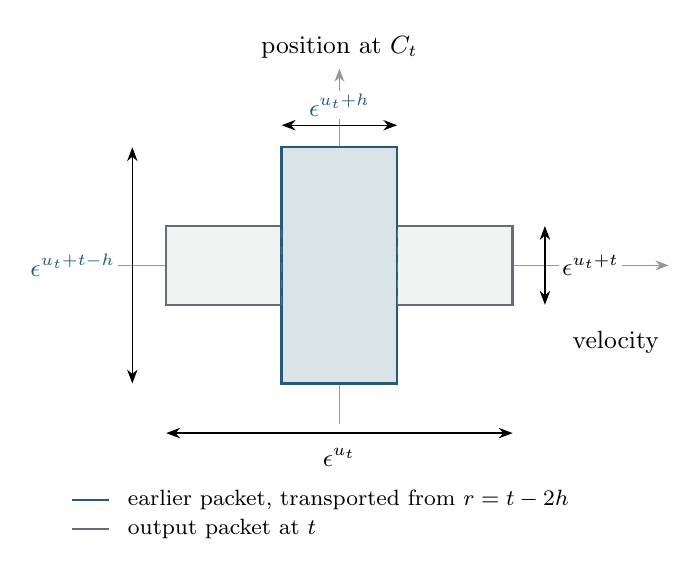
\begin{tikzpicture}[font=\small,>=Stealth,
  dimension/.style={<->,line width=0.45pt}]
  \draw[->,figuregray!70] (-3.05,0) -- (4.18,0);
  \node[anchor=north east] at (4.18,-0.71) {velocity};
  \draw[->,figuregray!70] (0,-2.02) -- (0,2.50)
    node[above,text=black] {position at $C_t$};
  \filldraw[fill=figuregray!9,draw=figuregray,line width=0.85pt]
    (-2.2,-0.5) rectangle (2.2,0.5);
  \filldraw[fill=figureblue!17,draw=figureblue,line width=0.85pt]
    (-0.73333,-1.5) rectangle (0.73333,1.5);
  \draw[figuregray,dashed,line width=0.45pt]
    (-0.73333,-0.5) -- (-0.73333,0.5);
  \draw[figuregray,dashed,line width=0.45pt]
    (0.73333,-0.5) -- (0.73333,0.5);
  \draw[dimension] (-0.73333,1.78) -- (0.73333,1.78)
    node[midway,above=2pt,text=figureblue,fill=white,inner sep=1pt] {$\eps^{u_t+h}$};
  \draw[dimension] (-2.2,-2.13) -- (2.2,-2.13)
    node[midway,below=2pt] {$\eps^{u_t}$};
  \draw[dimension] (-2.63,-1.5) -- (-2.63,1.5)
    node[midway,left=5pt,text=figureblue,fill=white,inner sep=1pt] {$\eps^{u_t+t-h}$};
  \draw[dimension] (2.61,-0.5) -- (2.61,0.5)
    node[midway,right=5pt,fill=white,inner sep=1pt] {$\eps^{u_t+t}$};
  \draw[figureblue,line width=0.85pt] (-3.4,-2.98) -- (-2.92,-2.98);
  \node[anchor=west,font=\footnotesize] at (-2.81,-2.98)
    {earlier packet, transported from $r=t-2h$};
  \draw[figuregray,line width=0.85pt] (-3.4,-3.35) -- (-2.92,-3.35);
  \node[anchor=west,font=\footnotesize] at (-2.81,-3.35)
    {output packet at $t$};
\end{tikzpicture}
\caption{One coordinate pair of packet uncertainty cells at a common
output anchor, with $0<h\le t/2$, $t\le\Planck$ and
$u_t=(\Planck-t)/2$.
The earlier packet has $u_r=u_t+h$: its velocity cell is finer by depth
$h$, while its transported position uncertainty is coarser by depth $h$.
Both displayed rectangles have the same area,
$\eps^{u_t+h}\eps^{u_t+t-h}
=\eps^{u_t}\eps^{u_t+t}=\eps^{\Planck}$.
The rectangles are drawn concentrically to compare their scales and
represent comparable widths after transport; fixed factors, shear and
subpower tail enlargements are suppressed.
An earlier packet can therefore contribute across several fine output
position cells.  Its transported center alone does not determine the
fine output position label.}
\label{fig:packet-cells}
\end{figure}


\subsection{The incoming fine-velocity information}

Here is the precise meaning of the velocity information carried between
steps.  At time \(t\), let
\[
 u_t=(\Planck-t)/2,\qquad
 P_f=(C_t,\text{isotropic velocity and position cells of width }
                  \eps^{u_t-h}).
\]
The position width in this formula is \(\eps^{t+u_t-h}\).
Fixed dilations and translations of the grids are allowed.  Additional
tags are allowed only if their conditional number, given the geometric
part of \(P_f\), is at most \(\eps^{-\alpha}\); their cost is included
in \(\alpha\).

In the elongated case \(n_f(P_f)\) is a unit normal, modulo sign, and
the normal of the aperture \(D\) is within \(C\eps^h\) of \(n_f(P_f)\).
The label \(W_f\) locates the velocity component along \(n_f(P_f)\)
in intervals of length \(\eps^{u_t}\).  In the isotropic case \(W_f\)
locates both velocity components at that precision.  An incoming
credit \(k_f\geq0\), with error \(\alpha_f\), means that on the
normalized law being used,
\begin{equation}
 \sup_w\PP(W_f=w\mid P_f=p)\leq
       \eps^{\,k_f-\alpha_f}
       \quad\text{for every \(p\) of positive probability}.
 \label{eq:incoming-packet-credit}
\end{equation}
In particular \(\Ent(W_f\mid P_f)\geq k_f-\alpha_f\).
On the first step we set \(k_f=0\) and impose no incoming direction
or fine-velocity condition.

We will use the following exact retention rule.  It specifies how
\eqref{eq:incoming-packet-credit} is maintained when selecting branches.

\begin{lemma}[Retention of a conditional probability bound]
\label{lem:packet-credit-retention}
Suppose a finite law satisfies
\(\PP(W=w\mid P=p)\leq\eps^{k-\alpha}\).
Let \(A\) have probability \(p_A>0\), and let \(\zeta>0\).
Under the law conditioned on \(A\), the set of fibers on which
\[
 \PP(A\mid P)<p_A\eps^\zeta
\]
has probability at most \(\eps^\zeta\).  On every remaining fiber,
\begin{equation}
 \PP(W=w\mid P,A)\leq
   \eps^{\,k-\alpha-\zeta-\logeps{1/p_A}}.
 \label{eq:credit-retention}
\end{equation}
Removing the exceptional fibers does not change this conditional
bound.  The same assertion holds when \(P\) includes other previously
fixed labels.
\end{lemma}

\begin{proof}
The exceptional probability, in the conditioned law, is
\[
 p_A^{-1}\sum_{\{p:\,\PP(A\mid P=p)<p_A\eps^\zeta\}}
       \PP(P=p)\PP(A\mid P=p)\leq\eps^\zeta.
\]
On a remaining fiber divide
\(\PP(W=w,A\mid P=p)\leq\PP(W=w\mid P=p)\)
by \(\PP(A\mid P=p)\).  Conditioning subsequently on a set of \(P\)
values does not alter the conditional law given \(P\).
\end{proof}

Every removal below is also a score split under
Section~\ref{sec:packet-composition}; its probability alone does
not control the remaining score.


\subsection{Constructing the finite cut}

A prepared cut starts with a boundary step from \(r=t-2h>0\) to \(t\),
with \(u_t>h\),
as supplied by Proposition~\ref{prop:boundary-alternatives}.
The current endpoint law will be denoted by \(\pi^{\rm in}\).
It is a probability law on a finite sample space \(\Omega\).
A sample \(\omega\) records \(O(\omega),D(\omega)\), all incoming
labels \(P_f,W_f\) and their extra tags when present, and any auxiliary
randomness already used to choose those labels.  In particular, an
incoming label need not be a deterministic function of \((O,D)\).
For any endpoint law \(\nu\) on \(\Omega\), write \(P_t(\nu)\)
for the score of the original input with its original masses.
If \(k_f>0\), the bound \eqref{eq:incoming-packet-credit} holds under
\(\pi^{\rm in}\), with its current error.  On the first step
\(k_f=0\).

The finite geometry is the following.  The endpoint shape has
\(a=u_t\) to depth error at most \(\eta\).  In the isotropic
alternative the apertures are isotropic and \(b_*=0\).  In the
elongated alternative \(b_*=b\), the endpoint aspect \(e=a-b\)
is at least \(e_0>0\).  In that case require
\begin{equation}
 C_*(h+\eta)<\gamma e_0 .
 \label{eq:repayment-eccentricity}
\end{equation}
The grids and aperture menu admit all coarsenings below.  We take
\(C_*\ge2\).  Thus in the elongated case
\(b\le u_t+\eta-e_0\le u_t-h\), after increasing \(C_*\) if
necessary; in the isotropic case \(b_*=0<u_t-h\).  We will use
\begin{equation}
 b_*\le u_t-h
 \label{eq:repayment-localizer-depth}
\end{equation}
when comparing the incoming coarse label with the localizer.

Use the fixed analytic, domain, depth, grid, and count bounds of
Section~\ref{sec:packet-composition}.  For supremum masses, fix at
each site a test within a fixed factor of the supremum and call its
mass \(m_O(f)\).  This changes any endpoint score by at most
\(C/\ell\), included in \(\mathcal R\), and the Bessel bounds are
uniform in these choices.  Apply the floor
\(m_O(f)\ge\eps^{A_0}\|f\|_2^2\) of
\eqref{eq:packet-output-floor} and the fixed-shape score splits,
recording their probabilities for credit retention.

Fix the depths, then \(\theta<h/10\) and \(\xi\).  By
\eqref{eq:repayment-localizer-depth},
\(\theta<(u_r-b_*)/4\), as required by
Lemma~\ref{lem:packet-decomposition}.  Choose its amplitude error
\(C_A\eps^A\|f\|_2\) with \(A>A_0/2+1\).  If \(Q_0\) bounds
all relevant count exponents, choose the coefficient cutoff
\begin{equation}
 B>2A+3Q_0+10 .
 \label{eq:repayment-coefficient-cutoff}
\end{equation}
uniformly over geometric localizers.  The later transport order
may be increased after this coefficient family is fixed.

For one geometric localizer \(J_0\), let \(\iota\) range over its
coefficient bins and greedy cap classes.  The associated whole class
is a finite set \(\mathcal T_\iota^{\rm all}\) of earlier atoms,
with coefficient mass bin \(m(\iota)\), cap maximum bin \(g(\iota)\),
and assigned cap \(E_\iota(T)\).  Lemma~\ref{lem:cap-class} gives
the cap upper bound on this set and the lower bound on each of its
whole assigned fibers.  At this point \(\iota\) indexes available
classes; no class has yet been assigned to an endpoint sample as its
final winner.  The buffer used next is chosen for all possible
contributors in this finite family, before any of its classes is
subdivided.

During preparation, a replacement loss is the increase in score
when the aperture is changed at fixed masses, evaluated on the
specified current marginal.  Section~\ref{sec:packet-composition}
supplies these losses from the current deficits and charges each
split.  This also applies to the two-copy marginals in the next
lemma, since adjoining the unsplit conditional copies preserves
the old marginal.

For every possible contributor, the velocity difference from its
output center is \(O(\eps^{u_t})\).  After referring the positions
to \(C_r\), their difference is
\[
 O(\eps^{r+u_t})+
 O(\eps^{-\theta}\eps^{r+u_r})
       =O(\eps^{r+u_t}),
 \qquad u_r=u_t+h,\quad \theta<h/10.
\]
Use isotropic cells with side \(L_{\rm grid}\) times
\(\eps^{u_t}\) in velocity and \(\eps^{r+u_t}\) in position,
where \(L_{\rm grid}\) is a sufficiently large fixed constant.
A uniformly random translation places any output center farther
than these possible differences from every face with probability
at least \(3/4\).  Averaging over translations therefore gives
one translation for which a part of at least that probability has
the coarse label
\[
 P=(C_r,V_{u_t},(X+(C_r-C_t)V)_{r+u_t})
\]
in common with every possible contributing earlier atom.
Retain this part as a score split and denote its normalized
endpoint law by \(\pi^{\rm buf}\).  Its probability and deficit
are charged by the finite selection rule above.  This completes
the geometric preparation in the isotropic case.

\begin{lemma}[Prediction of a normal from isotropic replacements]
\label{lem:orientation-prediction}
Assume the elongated geometry.  On \(\pi^{\rm buf}\), suppose the
replacement losses for the isotropic apertures of widths \(a\) and
\(b\) are included in \(C_*\eta\).  Take two copies
\((O,D),(O',D')\), independent conditional on \(P\), and set
\[
 A_{\rm sep}=\{\angle(n(D),n(D'))\ge\eps^{4h}\}.
\]
If this event has probability at least \(1/4\), require the same
replacement bounds on both marginals of the law conditioned on
\(A_{\rm sep}\).  Then there is a
deterministic normal \(n(P)\), defined on every coarse cell used
by the atom partition, such that
\[
 \angle(n(D),n(P))\le C\eps^{4h}
\]
on a part of \(\pi^{\rm buf}\)-probability at least \(3/4\).
\end{lemma}

\begin{proof}
Let \(e=a-b\), and let \(B_P\) be the isotropic coarsening of \(P\)
to width \(b\).  Grid list errors will be included in \(C_*\eta\).
Only \(2h\) extra depth for time and \(2h\) for each position
coordinate are missing from \(P\) in order to specify \(O\), so
\begin{equation}
 \Ent(O\mid P)\leq6h+C_*\eta.
 \label{eq:prediction-missing-data}
\end{equation}
Replacing \(D\) by the isotropic aperture of width \(a\) gives
\begin{equation}
 \Ent(P\mid D)\geq(1+\gamma)e-6h-C_*\eta.
 \label{eq:prediction-lower}
\end{equation}
Indeed the weight increases by \((1+\gamma)e\), and the new
conditional observation entropy is nonnegative.  Replacing \(D\)
by the isotropic width-\(b\) aperture at \(t\), which has at most
\(6h+C_*\eta\) information beyond \(B_P\), gives
\begin{equation}
 \Mut(P;D\mid B_P)\leq(1-\gamma)e+6h+C_*\eta.
 \label{eq:prediction-upper}
\end{equation}
Both inequalities are comparisons on the marginal law on which
they are invoked.

Suppose \(A_{\rm sep}\) has probability at least \(1/4\), and
condition the two-copy law on this event.
For the resulting law, conditional dependence of the two copies
given \(P\) is at most
\(\log(1/\PP(A_{\rm sep}))/\ell\leq(\log4)/\ell\).
This follows by comparing its density with the original conditional
product and using the chain rule for relative entropy.
The marginal replacement estimates
\eqref{eq:prediction-lower}--\eqref{eq:prediction-upper}
continue to hold with their charged conditional deficits.

Each aperture, referred to \(C_r\), constrains both columns to a
normal strip of width a fixed multiple of \(\eps^{a-C_*\eta}\).
Two such strips whose normals have angle at least \(\eps^{4h}\)
have intersection of diameter at most
\(C\eps^{a-4h-C_*\eta}\).
Covering both columns by \(P\) cells consequently gives
\begin{equation}
 \Ent(P\mid D,D')\leq16h+C_*\eta.
 \label{eq:prediction-intersection}
\end{equation}
Here a strip intersection is used separately for velocity and root
position, each in two dimensions; hence \(4(4h)=16h\).
The coarse label \(B_P\) has bounded ambiguity given either aperture.
The identity
\[
 \Mut(P;D'\mid D,B_P)-\Mut(P;D'\mid B_P)
 =\Mut(D;D'\mid P,B_P)-\Mut(D;D'\mid B_P)
\]
and conditional product comparison therefore imply that its left
side is at most \(C_*\eta\).
The first term is at least
\((1+\gamma)e-22h-C_*\eta\), by
\eqref{eq:prediction-lower} and
\eqref{eq:prediction-intersection}; the second is at most
\((1-\gamma)e+6h+C_*\eta\), by
\eqref{eq:prediction-upper} for the other marginal.
Thus \(2\gamma e\leq28h+C_*\eta\), contrary to the eccentricity
hypothesis after fixing \(C_*\).
It follows that the complementary angle-proximity event has
probability at least \(3/4\).  For each \(P=p\), choose one normal
maximizing the conditional mass of a ball of radius
\(C\eps^{4h}\).  Averaging the two-copy probability shows that the
single-copy part predicted by these normals has mass at least
\(3/4\).

On coarse cells of zero probability choose an arbitrary normal.
This extends the table \(n(P)\) to every cell that will index an atom
subdivision, without changing the asserted event.
\end{proof}


\subsection{The subclasses and the current endpoint law}

Retain the buffered and, in the elongated case, predicted-normal
parts just constructed.  The table \(n(P)\) and the translated grid
are now fixed.  Their selection probabilities, together with the
earlier mass-floor and shape selections, are included in one
preparation event \(A_{\rm pre}\) in the original sample space
\(\Omega\).  We will restore the incoming conditional probability
bound after the atom partition and the winning map have been fixed.

For an earlier atom \(T\), let \(P(T)\) be its buffered coarse cell.
In the elongated case first mark the atom according to whether the
normal of its assigned aperture \(E_\iota(T)\) lies within
\(2C\eps^h\) of \(n(P(T))\).  This divides each whole class into
aligned and misaligned atoms; both parts remain available when the
winner is chosen.  In the isotropic case no such mark is needed.

Let \(W(T)\) record the velocity at depth \(u_r=u_t+h\).  It records
the component along \(n(P(T))\) in the elongated case and both
components in the isotropic case.  These are the original depth
units; after subtracting \(b_*\), the fine spacing is
\(\eps^{u_r-b_*}\).  Within each marked part of
\(\mathcal T_\iota^{\rm all}\), and for each \(P\), bin
\[
 \logeps{\#\{T:(P(T),W(T))=(p,w)\}}
\]
with mesh \(\xi\).  Among fibers in one such size bin, bin the
logarithm of the number of represented \(W\)'s at \(P\), again with
mesh \(\xi\).  Write \(k\ge0\) for this second numerical tag and
\(d=1\) in the elongated case, \(d=2\) in the isotropic case.
For each resulting subclass and every represented \(P\),
\begin{equation}
 \eps^{-k+\xi}\leq \#\{W\mid P\}\leq\eps^{-k-\xi},
 \qquad k\leq dh+C\xi+\frac{\log C}{\ell}.
 \label{eq:velocity-fiber-regularity}
\end{equation}
The last bound covers a velocity cell of width \(C\eps^{u_t}\)
by cells of width \(\eps^{u_r}\) in \(d\) dimensions.
The sizes of two nonempty \((P,W)\) fibers in this subclass differ
by at most \(\eps^{-\xi}\).  Hence its uniform atom law satisfies
\begin{equation}
 \PP(W=w\mid P,J)\leq\eps^{k-2\xi}.
 \label{eq:prepared-velocity-probability}
\end{equation}
Here \(J\) will be the label of the subclass when it is chosen.
The subdivision groups the numerical fiber-size and \(k\) tags
across different \(P\)'s; \(P\) itself remains random in the
subclass and is not appended as an auxiliary value of \(J\).
This distinction keeps the later conditional cost of \(J\) small.

These are the final subdivisions that change atom sets.  Later tags,
such as total size, label a whole subclass.  Let \(S_\eps\) bound
the number of available subclasses at a geometric localizer; at
fixed depths \(\log S_\eps=o(\ell)\).  Their labels contain \(J_0\),
the \(\iota\) tags, the alignment mark when present, the two
numerical velocity tags, and any whole-subclass tags.  The winner map will choose one
such tuple \(J(\omega)\).  For its atom set \(\mathcal T_J\), set
\(\mathcal T_J^{\rm all}:=\mathcal T_\iota^{\rm all}\),
\(E(T):=E_\iota(T)\), and
\[
 N(J)=\#\mathcal T_J,\qquad
 N_{\rm all}(J)=\#\mathcal T_\iota^{\rm all},\qquad
 m(J)=m(\iota),\qquad g(J)=g(\iota).
\]
Thus \(N_{\rm all}\) still counts the whole greedy class before
alignment and velocity subdivision.  Its cap upper bound persists
on \(\mathcal T_J\); its assigned-fiber lower bound continues to
refer to the whole class.

Write \(\mathfrak a_O(\varphi)\) for the normalized pairing with
the fixed site test, so \(m_O(\varphi)=|\mathfrak a_O(\varphi)|^2\),
and \(h_J=\sum_{T\in\mathcal T_J}c_Tg_T\).  Put
\[
 q_0=C_A\eps^{A-A_0/2}<\tfrac12.
\]
Choose at each retained sample a subclass maximizing
\(|\mathfrak a_O(h_J)|\), breaking ties by a fixed rule.  All atom
sets, superpositions, and this map to \(J\) are now fixed.  Applied
to these final subclasses, \eqref{eq:packet-winner-mass} gives
\begin{align}
 |\mathfrak a_O(h_J)|
 &\ge\frac{1-q_0}{S_\eps}\sqrt{m_O(f)}
 \ge\frac{1-q_0}{S_\eps}\eps^{A_0/2}\|f\|_2,
 \label{eq:repayment-winner-floor}\\
 m_O(f)&\le (1-q_0)^{-2}S_\eps^2m_O(h_J)
          \le4S_\eps^2m_O(h_J).
 \label{eq:repayment-original-winning}
\end{align}
The mass-term loss
\(3\logeps{S_\eps}+3\logeps{1/(1-q_0)}\) is included in
\(\mathcal R\).  In the elongated case both alignment marks
participated in this choice.

After this finite menu, winner map, and coefficient cutoff are fixed,
Lemma~\ref{lem:packet-decomposition} allows one common transport power
\begin{equation}
 A_{\rm tr}>(B+Q_0+1)/2
 \label{eq:repayment-transport-order}
\end{equation}
for every retained subclass, without a new coefficient cutoff.
Its constants depend only on the fixed data and \(Q_0\).  This
order controls the alignment collapse and the later candidate
truncation, and is unchanged by subsequent subclass selections.

Take the endpoint law conditioned on \(A_{\rm pre}\).  If \(k_f>0\),
apply Lemma~\ref{lem:packet-credit-retention} to this event, using
its probability under \(\pi^{\rm in}\), and remove the exceptional
\(P_f\) fibers.
This changes the endpoint law and its full \(J\) marginal, while
leaving the atom sets, counts, \(g,m\), and winner map fixed.
The pointwise geometric and mass comparisons persist.  Apply
Proposition~\ref{prop:finite-packet-composition} anew to this
law; its new deficit inequality controls the mean
\(\EE\logeps{N_{\rm all}/N}\) under its new \(J\) marginal.

For each later numerical-tag or alignment restriction \(A\), use
its probability \(p_A\) in the current normalized law.  When
\(k_f>0\), repeat the retention lemma and the exceptional-fiber
score split.  In either case reapply composition with the same
frozen data.  Each retention application adds
\begin{equation}
 \zeta+\logeps{1/p_A}
 \label{eq:repayment-credit-cost}
\end{equation}
to the incoming error.  Use the weighted tag rule of
Section~\ref{sec:packet-composition} with its current union mass
\(p\) and shifted deficit \(R\): it supplies probability at least
\(p/(4S_\eps)\) and
conditional deficit at most \(4R/p\).  Only a prescribed finite
number of these operations is used.

The following exclusion determines which marked subclasses can remain.

\begin{lemma}[Alignment of the selected earlier aperture]
\label{lem:orientation-alignment}
For the elongated prepared cut, let \(\nu\) be a current endpoint
law supported on \(A_{\rm pre}\),
with the frozen winner map, and let \(d_i,R_t\) be its deficits and
bound from Proposition~\ref{prop:finite-packet-composition}.
Let \(B\) be a \(J\)-measurable event of misaligned winners, with
\(p=\nu(B)>0\), and put \(\varrho=\nu(\,\cdot\mid B)\).
In local coordinates write \(e=a-b\) and \((j,l)\) for the
assigned-cap widths.  Assume the common shape bins satisfy
\[
 l=e+h+O(\eta),\qquad l-j\ge e_0-O(\eta),
\]
as supplied by the boundary alternative, and that the prepared
packet, cap, and label errors are included in \(C_*\eta\).
Then
\begin{equation}
 p\,[2\gamma e_0-C_*(h+\eta)]
 \le \EE_\nu\!\left[\boldsymbol1_B(d_1+3d_2+3d_3)\right]
 \le 3R_t .
 \label{eq:alignment-misaligned-mass}
\end{equation}
Thus a positive bracket bounds the current probability of
misaligned winners by the current finite deficit.
\end{lemma}

\begin{proof}
Because \(B\) is \(J\)-measurable,
\(\varrho(\,\cdot\mid J)=\nu(\,\cdot\mid J)\) on \(B\), so the
local deficits are inherited.  Work at a fixed \(J\), subtract
\(b_*=b\) from widths, put \(\delta_J=d_2(J)+d_3(J)\), and let
\(M_j\) be the earlier isotropic depth-\(j\) cell.

For this comparison only, let
\(\mathcal O_J^\varrho=\{O(\omega):\varrho(\omega)>0,\ J(\omega)=J\}\).
For fixed \(P,C_t\), collapse the winning masses as
\[
 m^{\rm buf}_{P,C_t}
 =\sum_{\substack{O\in\mathcal O_J^\varrho\\O\mapsto(P,C_t)}}m_O(h_J).
\]
This sum counts each geometric site once, with the allowed bounded
lattice multiplicity.  Every tested site is buffered, so each of
its possible contributors shares its \(P\).  Write
\(\mathcal T_{J,P}=\{T\in\mathcal T_J:P(T)=P\}\) and
\(N_{J,P}=\#\mathcal T_{J,P}\).  The finite mass bound of
Proposition~\ref{prop:packet-trivial-growth}, with the fixed floor
and tail comparison, bounds the collapsed mass by \(mN_{J,P}\)
with the stated finite error.  Only then sample a contributor:
\[
 \varrho^P(\omega,T)=\varrho(\omega)
   \frac{\boldsymbol1_{\{T\in\mathcal T_{J(\omega),P(\omega)}\}}}
        {N_{J(\omega),P(\omega)}}.
\]
The floor and tail comparison ensure \(N_{J,P}>0\) on the tested
samples.  This kernel preserves the whole endpoint sample; its
atom marginal may be biased.  The following entropies are
conditional on \(J\) under this law.

The entropy calculation of
Proposition~\ref{prop:packet-trivial-growth} bounds \(P_J\) above by
\[
 \Ent(T)+\tfrac32\logeps{m}+
 \tfrac12\{\Ent(T\mid D)+(1-\gamma)e\}
 +\Ent(C_t\mid T)+C_*\eta.
\]
Here \(\Ent(T)\le\logeps{N}\) and
\(\Ent(C_t\mid T)\le2h+C_*\eta\).  For every sampled atom at \(P\)
and every aperture \(D\) over that \(P\), the buffered velocity and
root-position columns differ from those of the paired output by
at most the cell widths.  Since \(a=u_t+O(\eta)\), a fixed
enlargement of the root-referred cap of \(D\) contains all these
atoms, with the charged depth error.  The cap upper bound gives
\(\Ent(T\mid D)\le g-(1-\gamma)e+C_*\eta\).
The definitions of \(d_2,d_3\) give
\[
 P_J=A_J+2\betaq h+2\mathcal R-\delta_J\ge A_J-\delta_J.
\]
Comparing the two score bounds yields
\begin{equation}
 \Ent(T)\ge\logeps{N}-\delta_J-C_*(h+\eta),\qquad
 \Ent(T\mid D)\ge g-(1-\gamma)e-2\delta_J-C_*(h+\eta).
 \label{eq:alignment-biased-entropy}
\end{equation}

Before subdivision the number of distinct assigned \(E\) labels
is at most
\(\eps^{-\logeps{N_{\rm all}}+g-w(j,l)-C_*\eta}\), by the
whole-class fiber lower bound of Lemma~\ref{lem:cap-class}.
Since \(E\) is assigned deterministically to \(T\),
\begin{equation}
 \Ent(T\mid E)\ge
 g-w(j,l)-d_1(J)-\delta_J-C_*(h+\eta).
 \label{eq:alignment-assigned-entropy}
\end{equation}
The whole-fiber count has thus cost \(d_1(J)\) for the retained,
possibly biased law.

On \(A_{\rm pre}\), the normal of \(D\) is within \(C\eps^{4h}\)
of \(n(P)\).  A misaligned \(E\) therefore makes angle at least
\(C\eps^h\) with it.  Their two column intersections fit isotropic
caps of depth \(e-C_*h-C_*\eta\), so
\[
 \Ent(T\mid D,E)\le g-2e+C_*(h+\eta).
\]
Subtracting from \eqref{eq:alignment-assigned-entropy} and using
\(l=e+h+O(\eta)\) gives, for fixed \(J\),
\[
 \Mut(T;D\mid E)\ge
 (1+\gamma)(e-j)-d_1(J)-\delta_J-C_*(h+\eta).
\]
Average under \(\varrho_J\), absorbing the common-bin errors:
\begin{equation}
 \Mut_{\varrho^P}(T;D\mid E,J)\ge
 (1+\gamma)(e-j)-\EE_\varrho(d_1+\delta_J)-C_*(h+\eta).
 \label{eq:alignment-information-lower}
\end{equation}
As \(E\) is a function of \(T\) given \(J\), and determines \(M_j\) up to
the charged lists,
\[
 \Mut_{\varrho^P}(T;D\mid E,J)
 \le \Mut_{\varrho^P}(T;D\mid M_j,J)+C_*\eta.
\]

For the reverse estimate, coarsen \(D\) to widths \(0,j\), using
the center of \(M_j\).  Its normal projection is confined by the
coarsened strip, and the tangent width is zero-depth, so the
resulting labels form a charged list determined by \(D\).
Enlarge each rectangle by a fixed factor to contain the entire
\(M_j\) cell; its projections are bounded by its diagonal.
The enlargement depends only on the rectangle label.  Resample it
conditional on \((M_j,J)\), independently of \(T\), and call it
\(U\).  It is faithful for every atom in that cell, has weight
\((1-\gamma)j\), and the cap bound gives on each \(J\) fiber
\[
 \Mut(T;U)\ge \Ent(T)-g+(1-\gamma)j-C_*\eta.
\]
Adjoin these kernels under \(\varrho_J\), retaining the notation
\(\varrho^P\).  The joint law of the enlarged coarsening and \(M_j\) is
preserved on each fiber.  Since \(M_j\) is a function of \(T\) given \(J\),
\[
 \Mut_{\varrho^P}(M_j;D\mid J)
 \ge \Mut_{\varrho^P}(M_j;U\mid J)-C_*\eta
 =\Mut_{\varrho^P}(T;U\mid J)-C_*\eta.
\]
Average the cap bound and the second inequality in
\eqref{eq:alignment-biased-entropy}.  Combining them with this
display gives
\begin{equation}
 \Mut_{\varrho^P}(T;D\mid M_j,J)\le
 (1-\gamma)(e-j)+2\EE_\varrho\delta_J+C_*(h+\eta).
 \label{eq:alignment-information-upper}
\end{equation}
The lower and upper bounds imply
\[
 2\gamma(e-j)\le
 \EE_\varrho[d_1+3(d_2+d_3)]+C_*(h+\eta).
\]
The common shape bins give \(e-j\ge e_0-h-O(\eta)\).
Multiply by \(p\), use
\(p\EE_\varrho[\cdot]=\EE_\nu[\boldsymbol1_B\,\cdot]\), and use nonnegativity
of the \(d_i\) and \eqref{eq:finite-packet-deficits}.  This proves
\eqref{eq:alignment-misaligned-mass}.
\end{proof}

For the elongated application, first select a branch with qualifying
common earlier shape bins by the weighted rule, perform credit
retention when needed, and recompose.  Let \(\nu\) be this current
law and let \(B\) be all its misaligned winners.  This event is
\(J\)-measurable.  If \(\nu(B)=0\), the law is already aligned;
otherwise \eqref{eq:alignment-misaligned-mass} applies to its
entire current mass.  At sufficiently small current deficit,
the aligned complement has positive probability, tending to one
with the positive gap fixed.  Restrict to that complement, then
apply the current-law retention and recomposition rule.
In either alternative, apply the same rule to any remaining common
numerical-bin selections and recompose after the last restriction.  Denote
the resulting endpoint law on \(\Omega\) by \(\pi\), and now set
\(P_t=P_t(\pi)\), the score of the original input with its original masses.
Every final elongated winning class is aligned.
The buffered property, and prediction when present, persist pointwise.
The incoming bound is
\begin{equation}
 \sup_w\pi(W_f=w\mid P_f=p)
 \le \eps^{k_f-\alpha_f}
 \quad\text{for every \(p\) with \(\pi(P_f=p)>0\)},
 \label{eq:repayment-selected-credit}
\end{equation}
where \(\alpha_f\) includes the initial error and the sum of
\eqref{eq:repayment-credit-cost}.  When \(k_f=0\), this estimate
will be replaced by nonnegativity of conditional mutual information.

Every expectation in the rest of this cut uses the selected marginal
\(\pi_J\), unless a different law is explicitly displayed.  In
particular, set
\begin{align}
 d_1(J)&=\logeps{N_{\rm all}(J)/N(J)},\nonumber\\
 A_J&=\logeps{N(J)}+\tfrac32\logeps{m(J)}+\tfrac12g(J),\nonumber\\
 K_r^*(\pi)&=\Ent_\pi(J)+b_*+
   \EE_\pi\left[\logeps{N_{\rm all}(J)}
                  +\tfrac32\logeps{m(J)}+\tfrac12g(J)\right],
 \nonumber\\
 B_r&=\Ent_\pi(J)+b_*+\EE_\pi A_J
       =K_r^*(\pi)-\EE_\pi d_1 .
 \label{eq:repayment-benchmark}
\end{align}
The last equality is exact.  The number \(B_r\) is a benchmark
formed with retained counts; it is not asserted to be an earlier
score.
For the final composition law, put
\(\Delta_t=K_0+\betaq t-P_t\).  Its current \(d_0\) gives
\begin{equation}
 B_r+2\betaq h-P_t
 =\Delta_t+2\mathcal R-d_0-\EE_\pi d_1
 \le\Delta_t+2\mathcal R .
 \label{eq:repayment-input-bridge}
\end{equation}

The earlier whole-class law and the returned retained-class law are,
respectively,
\begin{equation}
 \mu^{\rm all}(J,T)=\pi_J(J)
   \frac{\boldsymbol1_{\{T\in\mathcal T_J^{\rm all}\}}}{N_{\rm all}(J)},
 \qquad
 \mu(J,T)=\pi_J(J)
   \frac{\boldsymbol1_{\{T\in\mathcal T_J\}}}{N(J)}.
 \label{eq:repayment-earlier-laws}
\end{equation}
Both use the selected marginal \(\pi_J\).  Their observations are
the sites of \(T\) at time \(r\), and their masses are coefficient
tests of the original input \(f\).  With assigned caps \(E(T)\),
finite composition gives
\begin{align}
 P_r^{\rm all}&\ge K_r^*(\pi)-\mathcal R,\nonumber\\
 P_r^{\rm ret}&\ge K_r^*(\pi)-\tfrac32\EE_\pi d_1-\mathcal R
       =B_r-\tfrac12\EE_\pi d_1-\mathcal R .
 \label{eq:repayment-earlier-scores}
\end{align}
In the elongated case \(\mu\) continues the aligned assigned cap.
In the isotropic case the same atom law uses the exact isotropic boundary aperture
of width \(u_r\).  The horizon and packet menu include this cap by
Proposition~\ref{prop:boundary-alternatives}.  With \(b_*=0\),
the isotropic score satisfies the separate bound
\begin{equation}
 P_r^{\rm iso}\ge
 B_r-\tfrac12\EE_\pi(g-2u_r)-C\mathcal R .
 \label{eq:repayment-isotropic-score}
\end{equation}
This uses weight \(2u_r\) and nonnegative conditional entropy,
independently of the assigned-fiber gain.  A charged selection fixed
the common \(g\) bin, and the final credit trim, when needed,
preserved its pointwise support before \(\pi\) was named.  Thus \(g-2u_r\) has
the required small error under the displayed expectation.

Finally, \eqref{eq:prepared-velocity-probability} applies under
\(\mu(\,\cdot\mid J)\).  Since the numerical \(k\) tags are common
bins under \(\pi_J\), averaging in \(J\) gives
\begin{equation}
 \mu(W=w\mid P=p)\le\eps^{k-C_*\eta}
 \quad\text{for every \(p\) with \(\mu(P=p)>0\)}.
 \label{eq:repayment-outgoing-credit}
\end{equation}
This statement holds for either earlier aperture assignment under
\(\mu\), which is uniform within each retained class.


\subsection{From winning masses to candidate masses}

Before stating the repayment estimate, we finish the finite comparison
of masses that its proof will use.  Work in the translated coordinates
of a selected localizer \(J\), put \(u=u_t-b_*\), and write
\[
 \rho=\eps^u,\qquad s=\eps^{u+h},\qquad
 \sigma=\eps^{u+2h}=s^2/\rho,\qquad \lambda_{\rm loc}=s^{-2}.
\]
The buffered \(P\) cell has width \(\rho\).  Let \(Q=Q(J,O)\) record
\(P,C_t\), and the position cell of side \(s\) at \(C_t\).
For each such \(Q\), let \(\mathcal T_{J,Q}\subset\mathcal T_J\)
consist of the atoms at this \(P\) whose transported positions are
within \(C_0 R s\) of that cell, where \(R=\eps^{-\theta}\)
and \(C_0\) is a fixed constant large enough for the transport and
cell-boundary enlargements.  Absorb \(C_0\) into the fixed constants
in the coherence estimates.
Write \(N_{J,Q}=\#\mathcal T_{J,Q}\) and
\[
 h_{J,Q}=\sum_{T\in\mathcal T_{J,Q}}c_Tg_T.
\]
Let \(Z=Z(J,O)\) add to \(Q\) the output position at precision
\(\sigma\) along \(n(P)\) in the elongated case and in both
directions in the isotropic case.  These labels are functions of the
geometric endpoint observation and the fixed grid and normal table;
they do not include the arbitrary extra labels carried by \(\omega\).
On the full sample space write \(Q(\omega)=Q(J(\omega),O(\omega))\)
and likewise for \(Z(\omega)\).

The winning superposition \(h_J\) is fixed, while \(h_{J,Q}\)
depends on \(Q\).  On every retained endpoint site, the buffered
property and the transport order fixed after the winning map give
\begin{equation}
 |\mathfrak a_O(h_J)-\mathfrak a_O(h_{J,Q(J,O)})|
       \le C_{\rm tr}\eps^{A_{\rm tr}}\|f\|_2 .
 \label{eq:repayment-winning-candidate-tail}
\end{equation}
The coefficient and count comparison in the original construction
is still available: the squared summed tail has exponent beyond
\(B+1\) after the \(Q_0\) count loss.  For the score we use the
stronger information that the winning amplitude itself has the
floor \eqref{eq:repayment-winner-floor}.  Set
\[
 q_{\rm tr}=
 \frac{C_{\rm tr}S_\eps}{1-q_0}
       \eps^{A_{\rm tr}-A_0/2}.
\]
The choices \(B>2A+3Q_0+10\), \(A>A_0/2+1\), and
\eqref{eq:repayment-transport-order}, together with the subpower
bound on \(S_\eps\), make \(q_{\rm tr}\to0\) at fixed finite
parameters.  Choose \(\eps\) small enough that \(q_{\rm tr}<1/2\).
Equations \eqref{eq:repayment-winner-floor} and
\eqref{eq:repayment-winning-candidate-tail} then imply
\begin{equation}
 m_O(h_J)\le(1-q_{\rm tr})^{-2}m_O(h_{J,Q(J,O)}).
 \label{eq:repayment-winning-candidate}
\end{equation}
In particular \(m_O(h_{J,Q(J,O)})>0\) and \(N_{J,Q(J,O)}>0\) on
every retained sample.  Replacing the winning mass by this
candidate-truncated mass costs at most
\begin{equation}
 3\logeps{1/(1-q_{\rm tr})}
 \label{eq:repayment-candidate-score-cost}
\end{equation}
in the score's mass term.  This cost is included in \(\eta\).

For a fixed \(J,Q\), define
\begin{equation}
 m_Z=\sum_{\substack{O\mapsto Z\\ O\ {\rm in\ the\ localizer}}}
             m_O(h_{J,Q}) .
 \label{eq:repayment-candidate-mass}
\end{equation}
The sum uses every geometric output site mapping to \(Z\) once,
with the allowed bounded lattice multiplicity and its chosen
site-dependent amplitude; it does not sum over copies of a site in
\(\Omega\).  Because \(Z\) includes \(Q\), the entire fiber uses
one input \(h_{J,Q}\).  Thus \(m_Z\) is exactly the
candidate-truncated mass to which the next lemma applies.
The input \(h_{J,Q}\) varies with \(Q\).  These masses are used
only to bound an entropy expression under \(\pi\); they are not
treated as a new admissible packet system for a growth estimate.

\subsection{The repayment estimate}

The prepared cut supplies \(\mu\) and the capacity bound
\eqref{eq:velocity-fiber-regularity}.  The remaining estimate shows
that a near-maximal endpoint score increases the fine-velocity credit.

\begin{proposition}[Finite packet repayment]
\label{prop:finite-repayment}
Fix \(0<\gamma<1\) and a comparison rate
\(b_{\mathrm q}\in[0,1]\).  For the prepared cut constructed above,
let \(\eta\) bound the composition budget \(\mathcal R\),
\(\theta+\xi+(\log C)/\ell\), all logarithmic class, winner, tail,
and label costs, the current mean \(\EE_\pi d_1\), and the finite
classical growth error on the fixed class of lines, after a fixed
increase of \(C_*\).  The selected endpoint and earlier replacement
and composition deficits required in the construction are at most
\(\eta\) on their specified current laws, including the two
conditional prediction marginals.  The common shape and count bins
have width at most \(\eta\); in the isotropic case they also give
the error in \eqref{eq:repayment-isotropic-score}.
When \(k_f>0\), assume \eqref{eq:repayment-selected-credit} under
\(\pi\) with its accumulated error \(\alpha_f\le\eta\).
Finally suppose
\begin{equation}
 P_t\ge B_r+2b_{\mathrm q}h-\Delta .
 \label{eq:repayment-saturation-input}
\end{equation}
Then the prepared statistic \(P,n(P),W,k\) under \(\mu\) satisfies
\begin{equation}
 0\le k\le d h+C_*\eta,\qquad
 k\ge k_f+(4b_{\mathrm q}-2\gamma)h-2\Delta-C_*\eta,
 \quad
 d=\begin{cases}1&\text{elongated},\\2&\text{isotropic}.
                 \end{cases}
 \label{eq:finite-packet-repayment}
\end{equation}
Its pointwise probability bound is
\eqref{eq:repayment-outgoing-credit}.  In the elongated case the
continued aperture normal is within \(C\eps^h\) of \(n(P)\).
The returned score satisfies \eqref{eq:repayment-earlier-scores}
in that case and \eqref{eq:repayment-isotropic-score} in the
isotropic case.  All these bounds are finite at fixed \(\eps\).
\end{proposition}

\subsection{A coherent estimate on the full set of output sites}

We next prove the mass estimate before introducing any positive law
on candidate packets.  The output amplitudes may be chosen separately
at every site.

\begin{lemma}[Packet coherence on a strip or a cell]
\label{lem:packet-coherence}
Use local coordinates with root time \(r\), endpoint duration \(2h\),
and put
\[
 \rho=\eps^u,\qquad s=\eps^{u+h},\qquad
 \sigma=\eps^{u+2h}=s^2/\rho,\qquad
 \lambda_{\rm loc}=s^{-2}.
\]
Fixed multiplicative errors in these relations change only constants.
Let \(P\) be a buffered isotropic cell of width \(\rho\).
Let \(Q\) specify \(P,C_t\) and a position cell of side \(s\) at
\(C_t\).  Candidate atoms have this \(P\), velocity spacing \(s\),
earlier position spacing \(s\), and transported position within
\(Rs\) of that cell, where \(R=\eps^{-\theta}\).
Let \(N_Q\) be their number, and suppose
\[
 |c_T|^2\leq\eps^{-\xi}m.
\]
Partition their velocities into \(K\leq\eps^{-k-\xi}\) bins of
width \(s\), in a fixed normal direction for \(d=1\) or in both
directions for \(d=2\).
Let \(Z\) add to \(Q\) the output position at precision \(\sigma\)
in those \(d\) directions.  Let \(m_Z\) be the sum of squared
packet tests over all output sites mapping to \(Z\), on the input
truncated to these candidates.  Then
\begin{equation}
 \sum_{Z\mid Q}m_Z\leq C\eps^{-\xi}N_Qm,\qquad
 m_Z\leq C\eps^{dh-k-2\theta-2\xi}N_Qm.
 \label{eq:finite-coherence}
\end{equation}
The constant is uniform over all admissible choices of the
site-dependent amplitudes.  Without candidate truncation, the
square root of the mass estimate has the additive tail error
provided by Lemma~\ref{lem:packet-decomposition}.
\end{lemma}

\begin{proof}
The first inequality is the synthesis Bessel estimate followed by
the analysis Bessel estimate of Lemma~\ref{lem:packet-bessel}.
It holds for any subset of output sites and any subset of atoms.

Suppose first that \(d=2\).  If \(A_{OT}\) is the normalized
atom/test matrix, then
\[
 |A_{OT}|\leq C\rho^{-1}\|g_T\|_1
          \leq C s/\rho=C\eps^h.
\]
A full velocity bin contains a bounded number of velocity lattice
centers.  At each such center the proximity condition leaves at
most \(CR^2\) position centers.  Each \(Z\) contains a bounded
number of output sites.  Cauchy--Schwarz first within one bin
and then across its \(K\) bins gives
\[
 m_Z\leq CKR^2\eps^{2h}\sum_T|c_T|^2
       \leq C\eps^{2h-k-2\theta-2\xi}N_Qm.
\]

For \(d=1\), write \(n\) for the bin normal and \(\tau\) for its
orthogonal unit tangent.  Fix one velocity bin \(W\).
There are at most \(CR^2\) candidate atoms per tangent velocity
interval of length \(s\).  We claim
\begin{equation}
 \sum_{O\mapsto Z}\left|
       \sum_{T\in W}c_T A_{OT}\right|^2
 \leq CR^2\eps^h\sum_{T\in W}|c_T|^2.
 \label{eq:one-bin-strip}
\end{equation}

Here are details that also justify using all output sites with
independently chosen amplitudes.  Write \(v=V_P+\rho z\) on a
common bounded patch and surround each output center \(X_O\)
by a square \(B_O\) of side comparable to \(\sigma\).
For \(x\in B_O\), remove the scalar value at \(v=V_P\) from
\[
 \psi_O((v-V_O)/\rho)
 \exp\{i\lambda_{\rm loc}
       [\Phi(C_t,X_O,v)-\Phi(C_t,x,v)]\}.
\]
All derivatives in \(z\) are uniformly bounded, because
\(\lambda_{\rm loc}\rho\sigma=1\).
A common bump and a Fourier series on a fixed enlarged patch
therefore give coefficients \(b_\nu(O,x)\) satisfying
\[
 |b_\nu(O,x)|\leq C_M(1+|\nu|)^{-M}
\]
uniformly in both \(O\) and \(x\).
Weighted Cauchy--Schwarz bounds the squared transform at \(X_O\)
by a fixed rapidly summable combination of squared transforms
at \(x\), each with a common bump and a linear modulation
\(e^{i\nu\cdot(v-V_P)/\rho}\).
These factors are independent of \(x\).
No derivatives with respect to the site index have been used.

Integrate this bound on \(B_O\), divide by its area, and sum.
The squares have bounded overlap, and their union lies in a
strip of normal width \(C\sigma\) and tangent length \(Cs\).
The normalization outside the resulting continuous position
integral is
\begin{equation}
 \rho^{-2}\sigma^{-2}=s^{-4}.
 \label{eq:strip-normalization}
\end{equation}
It is enough to prove the estimate for each of the common
bump/modulation factors, uniformly in its Fourier index; the
factor has bounded modulus and is independent of \(x\).

For fixed normal position, integrate against a smooth majorant
of the tangent interval of length \(Cs\).  For velocities in
the same \(W\), their normal difference is \(O(s)\).  Symmetry
and uniform definiteness of \(\partial_p\zeta\) give
\[
 \partial_\tau\{\Phi(C_t,x,v)-\Phi(C_t,x,v')\}
       =\tau^{\mathsf T}A(x,v,v')(v-v'),
\]
where \(A\) is an average of those definite matrices.
If the tangent separation is a sufficiently large multiple of
\(s\), this derivative has magnitude at least
\(c|(v-v')\cdot\tau|\).
Higher \(x\)-derivatives are bounded by \(C_j|v-v'|\).
Repeated integration by parts in the rescaled tangent variable
thus bounds its kernel by
\[
 C_Ms\left(1+\frac{|(v-v')\cdot\tau|}{s}\right)^{-M}.
\]
For smaller separation the same bound, with another constant,
follows directly by integration over the interval.
Earlier normalized atoms have \(L^1\) norm at most \(Cs\).
Including the normal integration and
\eqref{eq:strip-normalization}, the corresponding Gram entry
is therefore at most
\[
 C_Ms^{-4}\sigma s\,s^2
  \left(1+\frac{|(V_T-V_{T'})\cdot\tau|}{s}\right)^{-M}
 =
 C_M\eps^h
  \left(1+\frac{|(V_T-V_{T'})\cdot\tau|}{s}\right)^{-M}.
\]
The possible overlap of velocity supports changes only the
constant in this estimate.  Sum the rapidly decreasing kernel
over tangent intervals, using the multiplicity \(CR^2\).
The Schur bound proves \eqref{eq:one-bin-strip}.
Finally Cauchy--Schwarz over the \(K\) bins proves the second
inequality of \eqref{eq:finite-coherence} for \(d=1\).
\end{proof}


\subsection{The candidate law and its entropy bound}

We now prove Proposition~\ref{prop:finite-repayment}.
For a value \(J=j\) of positive \(\pi_J\)-probability, let
\(\pi_j\) denote the selected endpoint law conditional on \(J=j\).
Define the finite entropy expression
\[
 \mathcal E_j=
 \Ent_{\pi_j}(Z)+\tfrac12\Ent_{\pi_j}(Z\mid D)
 +\tfrac32\EE_{\pi_j}\logeps{m_Z}
 +\tfrac12\EE_{\pi_j}w_{\rm loc}(D).
\]
All entropies here concern the displayed geometric observations,
rather than the entire sample \(\omega\).  The latter carries
extra labels only so that later augmentation preserves them.
Finite composition first compares the original score with the
conditional winning scores.  Equation
\eqref{eq:repayment-winning-candidate} then replaces their masses
by the candidate-truncated masses.  Finally, conditional log-sum
on each \(O\mapsto Z\) fiber bounds the two entropy--mass terms
by those in \(\mathcal E_j\).  The unconditional fiber calculation
uses all sites mapping to \(Z\); conditional on \(D\), its support
is a subset of those sites.  Thus
\begin{equation}
 P_t\le \Ent_\pi(J)+b_*+\EE_{\pi_J}\mathcal E_J
       +\mathcal R+3\logeps{1/(1-q_{\rm tr})}.
 \label{eq:repayment-candidate-expression}
\end{equation}
This is a comparison of finite expressions under the same endpoint
law.  No growth bound has been applied to the \(Q\)-dependent inputs.

Lemma~\ref{lem:packet-coherence} now gives its two exact bounds for
the masses \(m_Z\) in \eqref{eq:repayment-candidate-mass}.
Only after these analytic inequalities do we introduce a positive
candidate law.  Adjoin an earlier atom to the full endpoint sample by
\begin{equation}
 \widetilde\pi(\omega,T)=\pi(\omega)
   \frac{\boldsymbol1_{\{T\in\mathcal T_{J(\omega),Q(\omega)}\}}}
        {N_{J(\omega),Q(\omega)}} .
 \label{eq:repayment-candidate-law}
\end{equation}
The denominator is positive on every sampled value, as proved above.
This law has exactly the endpoint marginal \(\pi\), including
\(P_f,W_f\) and every stochastic incoming tag.  Conditional on
\((J,Q)\), the atom is uniform on the candidate set and independent
of every other endpoint label.  Its marginal on atoms is generally
biased; it is different from \(\mu\), which is uniform within each
retained class.

For the next calculation fix \(J=j\), and write \(\Ent_j,\EE_j\)
for entropy and expectation under
\(\widetilde\pi(\,\cdot\mid J=j)\).  Put
\[
 B_{1,j}=\EE_j\logeps{N_{J,Q}},\qquad
 S_{t,j}=\Ent_j(C_t\mid T),\qquad
 \mathcal M_j=\EE_j\logeps{m_Z}.
\]
Since \(Z\) includes \(Q\), the sampling rule gives exactly
\[
 \Ent_j(T\mid Z,D)=\Ent_j(T\mid Z)=B_{1,j}.
\]
Candidate proximity gives
\(\Ent_j(Q\mid T,C_t)\le C_*\eta\).  It also gives
\(\Ent_j(Z\mid T,D)\le C_*\eta\).
For the latter bound, \(T,C_t\) locate the position to precision
\(s\), while \(D\) supplies its normal component at precision
\(\sigma\).  In the elongated case the current prediction
\(\angle(n(D),n(P))\le C\eps^{4h}\) moves a residual of size
at most \(\eps^{-\theta}s\) by at most
\(C\eps^{4h-\theta}s< C\sigma\).
In the isotropic case the aperture supplies both fine components.
The remaining costs are the stated lists and boundary-depth errors.

The chain rule gives
\begin{align}
 \Ent_j(Z)&\le \Ent_j(T)-B_{1,j}+S_{t,j}
                 +\Ent_j(Z\mid Q)+C_*\eta,
 \label{eq:repayment-entropy-chain-one}\\
 \Ent_j(Z\mid D)+B_{1,j}
       &\le \Ent_j(T\mid D)+C_*\eta.
 \label{eq:repayment-entropy-chain-two}
\end{align}
Conditional log-sum applied to the aggregate coherence bound, and
the logarithm of its pointwise bound, respectively give
\begin{align*}
 \Ent_j(Z\mid Q)+\mathcal M_j
     &\le B_{1,j}+\logeps{m(j)}+C_*\eta,\\
 \mathcal M_j&\le B_{1,j}+\logeps{m(j)}+k-dh+C_*\eta .
\end{align*}
Use the first inequality with coefficient \(1\) and the second
with coefficient \(1/2\) in
\eqref{eq:repayment-entropy-chain-one}--\eqref{eq:repayment-entropy-chain-two}.
Every occurrence of \(B_{1,j}\) cancels.  The result is
\begin{equation}
 \mathcal E_j\le
 \Ent_j(T)+\tfrac32\logeps{m(j)}
 +\tfrac12\{\EE_jw_{\rm loc}(D)+\Ent_j(T\mid D)
                    +2S_{t,j}+k-dh\}+C_*\eta .
 \label{eq:coherent-entropy-repayment}
\end{equation}
Here the common \(k\) bin absorbs its stated finite bin error.

We assemble these conditional kernels under \(\pi_J\) before
using incoming information.  Averaging
\eqref{eq:coherent-entropy-repayment} gives
\begin{align}
 \EE_{\pi_J}\mathcal E_J
 &\le \Ent_{\widetilde\pi}(T\mid J)
       +\tfrac32\EE_\pi\logeps{m(J)}\notag\\
 &\quad+\tfrac12\bigl\{
       \EE_\pi w_{\rm loc}(D)
       +\Ent_{\widetilde\pi}(T\mid D,J)
       +2\Ent_{\widetilde\pi}(C_t\mid T,J)
       +k-dh\bigr\}+C_*\eta .
 \label{eq:coherent-entropy-repayment-averaged}
\end{align}
The incoming conditional probability bound will be used under this
assembled law, not separately on each \(J\) fiber.

\subsection{A faithful aperture and the incoming information}

The candidate atoms carry exact straight lines through their earlier
positions with their assigned velocities.  In a localizer \(J\),
let \(F_T\) record \(C_t\) and both columns of this line at
isotropic width \(u-h\) at the endpoint.  Its local position
precision is \(\eps^{u+h}=s\).  Thus \(F_T\) is a function of
\((T,C_t,J)\); conditional on \(J\), it need not be a function
of \(T\) alone.

In the elongated case coarsen the orientation of \(D\) and its
aperture data to widths \(0,u-h\), computing the latter from the
center given by \(F_T\).  In the isotropic case use widths
\(u-h,u-h\).  Denote this intermediate observation by \(Y\).
Transport proximity makes \(Y\) determined by \(D\), conditional
on \(J\), up to a list of size at most \(\eps^{-C_*\eta}\).

Enlarge each rectangle of \(Y\) by one fixed factor so that it
contains the entire corresponding isotropic \(F_T\) cell.  The
factor works for every orientation: projections of a square have
length at most its diagonal, and rounding the center adds only a
fixed grid spacing.  This costs at most \((\log C)/\ell\) in depth.
Call the enlarged label \(\bar Y\).  It is a function of \(Y\),
so it has the same conditional list bound from \(D\).
Let \(\kappa(g\mid F_T,J)\) be the conditional law of \(\bar Y\)
under \(\widetilde\pi\), and adjoin \(G\) by that kernel:
\[
 \widetilde\pi(\omega,T,G)
   =\widetilde\pi(\omega,T)\kappa(G\mid F_T,J).
\]
We keep the same notation for the augmented law.  It preserves the
entire old law of \((\omega,T)\) and the joint law of
\((F_T,J,\bar Y)\) with \(\bar Y\) replaced by \(G\).
The new \(G\) is independent of \(T\) conditional on \((F_T,J)\),
contains \(C_t\), and is faithful for every line with that
\(F_T,J\) value.  No \(T\)-dependent cell is appended to its label.

Apply Theorem~\ref{thm:classical-growth} in each localizer with
duration \(2h\) and horizon \(u+h\).  The strict eccentricity
condition, or \(b_*=0\) with \(u_t>h\), gives \(u>h\).
Its root caps have widths at most
\(u+h=u_r-b_*\), and the endpoint horizon \(a+t\le L\), with its
stated depth error, also places them inside the local packet menu.
For every such root test \(F\), the support upper bound gives
\[
 \Ent_j(T\mid F)+\EE_j w(F)\le g(j)+C_*\eta.
\]
This uses only the retained support, so it holds for the biased
candidate marginal.  The positive root supremum is consequently at
most \(g(j)-\Ent_j(T)+C_*\eta\).  Positive growth yields, on
each \(J=j\) fiber,
\begin{equation}
 \EE_j w(G)+\Ent_j(T\mid G)+2S_{t,j}
       \le g(j)+2\gamma h+C_*\eta .
 \label{eq:faithful-classical-bound}
\end{equation}
Averaging these inequalities under the same \(\pi_J\) as before,
\begin{equation}
 \EE_{\widetilde\pi}w(G)+\Ent_{\widetilde\pi}(T\mid G,J)
       +2\Ent_{\widetilde\pi}(C_t\mid T,J)
 \le \EE_\pi g(J)+2\gamma h+C_*\eta .
 \label{eq:faithful-classical-bound-averaged}
\end{equation}

All information in the remainder of this subsection is under the
assembled augmented law \(\widetilde\pi\).  Both \(D\) and \(G\)
contain \(C_t\), and \(F_T\) is a function of \((T,C_t,J)\).
The common time information cancels in the exact chain rule
\begin{align}
 \Mut(T;D\mid J)-\Mut(T;G\mid J)
 &=\Mut(F_T;D\mid C_t,J)-\Mut(F_T;G\mid C_t,J)
       \notag\\
 &\quad+\Mut(T;D\mid F_T,J)-\Mut(T;G\mid F_T,J).
 \label{eq:time-correct-information-splitting}
\end{align}
The last term is zero by the resampling kernel.  Data processing
for \(\bar Y\), followed by preservation of its joint law with
\((F_T,J)\), bounds the first line below by \(-C_*\eta\).
Therefore
\begin{equation}
 \Mut(T;D\mid J)-\Mut(T;G\mid J)
       \ge \Mut(T;D\mid F_T,J)-C_*\eta .
 \label{eq:information-before-credit}
\end{equation}

When \(k_f>0\), the preserved endpoint marginal supplies an
averaged information lower bound
\begin{equation}
 \Mut(T;D\mid F_T,J)\ge k_f-C_*\eta .
 \label{eq:credit-information}
\end{equation}
Here is the finite-list verification.  In absolute units,
\(F_T\) and \(P_f\) have identical velocity depth \(u_t-h\)
and position depth \(t+u_t-h\).  The candidate position differs
from the observed one by at most
\(\eps^{-\theta}\eps^{r+u_r}\), exactly an
\(\eps^{-\theta}\) multiple of that position unit, and the
velocity difference is \(O(\eps^{u_t})\).
The localizer has the coarser width in
\eqref{eq:repayment-localizer-depth}; its remaining tags have the
charged conditional count.  It follows that
\[
 \Ent(F_T,J\mid P_f)\le C_*\eta,\qquad
 \Ent(P_f\mid F_T,J)\le C_*\eta .
\]
Because \(\widetilde\pi_\Omega=\pi\),
\eqref{eq:repayment-selected-credit} still holds for its endpoint
labels.  It is not asserted after conditioning separately on \(J\).
The chain rule gives
\[
 \Ent(W_f\mid F_T,J)
 \ge \Ent(W_f\mid P_f)-\Ent(F_T,J\mid P_f)
 \ge k_f-C_*\eta .
\]

Neither coarse label alone determines \(W_f\).  The pairs
\((D,F_T,J)\) and \((T,F_T,J)\), however, each determine a
list of at most \(\eps^{-C_*\eta}\) possibilities.
First list the possible \(P_f\)'s supplied by \(F_T,J\).
For each listed value, \(n_f(P_f)\) is known, with no continuity
assumption on this function.  Use that value's coarse velocity center
as reference.  The remaining velocity has size
\(O(\eps^{u_t-h})\).  The incoming alignment of the normal of
\(D\) with \(n_f(P_f)\) is \(O(\eps^h)\), so changing between
them changes the measured component by \(O(\eps^{u_t})\), one
\(W_f\) unit.  Thus \(D\) resolves that component to the stated
list.  The exact velocity of \(T\) does so as well, since it differs
from the output velocity by \(O(\eps^{u_t})\).
For isotropic tests use both velocity coordinates.  Consequently
\[
 \Ent(W_f\mid D,F_T,J)+\Ent(W_f\mid T,F_T,J)\le C_*\eta .
\]
The elementary information inequality
\[
 \Mut(T;D\mid F_T,J)\ge
 \Ent(W_f\mid F_T,J)-\Ent(W_f\mid D,F_T,J)
                         -\Ent(W_f\mid T,F_T,J)
\]
proves \eqref{eq:credit-information}.  This is a conditional
information averaged over \(J\) under \(\widetilde\pi\), which is
exactly what the averaged bounds need.  If \(k_f=0\), use
nonnegativity of conditional mutual information instead.

Combining \eqref{eq:information-before-credit} and
\eqref{eq:credit-information} with
\eqref{eq:faithful-classical-bound-averaged} gives
\[
 \EE_{\widetilde\pi}w(G)+\Ent_{\widetilde\pi}(T\mid D,J)
       +2\Ent_{\widetilde\pi}(C_t\mid T,J)
 \le \EE_\pi g(J)+2\gamma h-k_f+C_*\eta .
\]
The weight change on each localizer is
\[
 w_{\rm loc}(D)-w(G)=
 \begin{cases}
 (1-\gamma)h+O(\eta),&d=1,\\
 2h+O(\eta),&d=2,
 \end{cases}
 \qquad
 w_{\rm loc}(D)-w(G)\le dh+C_*\eta .
\]
Also \(\Ent_{\widetilde\pi}(T\mid J)\le
\EE_\pi\logeps{N(J)}\), since every candidate lies in its retained
class.  Insert these bounds into
\eqref{eq:coherent-entropy-repayment-averaged}, then use
\eqref{eq:repayment-candidate-expression}.  The tail comparison
costs are included in \(\eta\), so after returning to the original
units,
\[
 P_t\le B_r+\gamma h+\tfrac12(k-k_f)+C_*\eta .
\]
Comparison with \eqref{eq:repayment-saturation-input} proves the
lower bound in \eqref{eq:finite-packet-repayment}.  Its upper
bound is \eqref{eq:velocity-fiber-regularity}.

Under \(\mu\) at time \(r\), \(P\) has depth \(u_t=u_r-h\)
and \(W\) has depth \(u_r\).  Thus
\eqref{eq:repayment-outgoing-credit} and the earlier aperture and
score bounds supply the next cut's incoming data.  That cut may use
a new atom decomposition: the coarse-label lists carry the observable
\(W\mid P\) bound, without identifying the two temporary candidate
populations.
This completes Proposition~\ref{prop:finite-repayment}.


\subsection{A finite backward chain}

Suppose, for a contradiction, that
\(\betaq>\gamma/2\), and set
\[
 c=4\betaq-2\gamma>0.
\]
Choose an integer \(q\) with \(qc>2\).
Proposition~\ref{prop:boundary-alternatives} supplies \(q\)
backward steps of a common positive length \(2h\), with
all times positive and \(u_t>h\).
In the forced alternative first take \(h\) sufficiently small
compared with the fixed aspect gap times \(\gamma\);
this verifies \eqref{eq:repayment-eccentricity}.
In the other alternative all the back tests are exactly isotropic.

Fix this chain and start with \(k_0=0\).  At cut \(i\), apply the
rule for a prepared cut and call its final endpoint law \(\pi_i\);
the returned \(\mu_i\) is the next endpoint law.  Let
\(\Delta_i,\eta_i\) be the actual selected errors for \(\pi_i\),
with \(J\)-averages under \((\pi_i)_J\).  They include the exceptional-fiber score splits and
the accumulated \(\zeta+\logeps{1/p_A}\) with every \(p_A\)
measured in its current law.  Choose the finitely many retention
parameters and current-law branches so this finite cost sum is
as small as required.

Within each fixed outer row \(j\), choose the finite inner parameters
\(\theta,\xi\) and the finitely many \(\zeta\)'s, then the initial
packet tail orders and coefficient cutoff, the later transport order,
and finally the precision \(\eps\).  These choices make the inner
errors, including both mass-comparison costs, arbitrarily small in
that row.  Finite composition and
\eqref{eq:repayment-input-bridge} leave the selected deficits bounded
by that row's \(\Delta_j\), with the fixed finite selection factors,
plus those inner errors.  With the target shape and \(g\) accuracies
fixed before choosing the late row, these factors are bounded across
the subsequence: only uniformly positive current masses of qualifying
unions and retained complements divide deficits, while individual
tag probabilities enter only logarithmic costs.
The selected deficits are not sent to zero inside the row.
Only then choose a sufficiently late outer row, with \(q\) and \(h\)
already fixed across the subsequence, and choose finite inner precision
in that row so that the total error bound below holds.  No transport
order uniform in unbounded outer aspect parameters is required.

Apply Proposition~\ref{prop:finite-repayment} with
\(b_{\mathrm q}=\betaq\).
Iteration of \eqref{eq:finite-packet-repayment} gives
\[
 k_q\geq qch-\sum_{i=1}^q(2\Delta_i+C_*\eta_i),
 \qquad
 k_q\leq2h+C_*\eta_q.
\]
Choose the finite errors so that
\[
 \sum_{i=1}^q(2\Delta_i+C_*\eta_i)+C_*\eta_q
                  <(qc-2)h.
\]
The two inequalities are incompatible.
Consequently \(\betaq\leq\gamma/2\), completing the proof of
Theorem~\ref{thm:packet-growth}.

\section{Oscillatory integrals and Bochner--Riesz multipliers}
\label{sec:multiplier}

We now turn packet growth into the multiplier bound. The first step is
an oscillatory integral estimate with loss $\lambda^\nu$ for every
$\nu>0$, uniform over fixed phase and amplitude classes. After a
change of variables, this gives norm
$O_{\delta,\nu}(\lambda^{-\delta+\nu})$ for a Bochner--Riesz kernel
shell of radius $\lambda$. Choosing $\nu<\delta$ makes the dyadic
shell sum converge. We keep the data bounds explicit because the
shell amplitudes vary with the scale.

\begin{theorem}[Oscillatory integral estimate]\label{thm:oscillatory-estimate}
Fix bounded input and output regions $K_v,K_x\subset\RR^2$.
For the input patch $K_v$, fix a class of smooth real phases satisfying
the phase assumptions of Section~\ref{sec:packet-structure}, with
common domain $[0,1]\times\RR^2\times U_v$, where $U_v$ is an open
neighborhood of $K_v$.  All enlarged patches required by the
decomposition, expressed in the original $v$ coordinates, are contained
in $U_v$ and obey common bounds.  The translated systems are considered
on the corresponding bounded rescaled patches described in that section,
with the resulting uniform bounds.  Throughout the phase domain,
\[
 \partial_v\Phi(c,x,v)=\zeta(v,x-cv).
\]
For each phase and each required original input patch $V$, the matrix
$\partial_p\zeta$ is symmetric and satisfies either
\[
 a_0I\le\partial_p\zeta(v,p)\le a_1I
 \qquad(v\in V,\ p\in\RR^2),
\]
or the same inequality with $-\partial_p\zeta$ in place of
$\partial_p\zeta$, with common constants $a_0>0$ and $a_1$ for the
class.  On these original patches, every mixed $v,p$ derivative of total
order $j$ of this matrix is bounded by $A^{j+1}(j!)^3$ for a common
$A\ge1$.  Fix these constants and all the seminorm bounds of a class of
smooth amplitudes $B$ supported in
$[0,1]\times K_x\times K_v$.  For every $\nu>0$ there is a constant
$C_\nu$, depending only on these fixed data and $\nu$, such that, for
every $\lambda\ge2$, every phase and amplitude in the specified classes,
and every $f\in L^3(\RR^2)$ supported in $K_v$,
\begin{equation}\label{eq:oscillatory-estimate}
 \left\|E_\lambda f\right\|_{L^3([0,1]\times K_x)}
 \le C_\nu\lambda^{-1+\nu}\|f\|_3,
 \qquad
 E_\lambda f(c,x)=\int e^{i\lambda\Phi(c,x,v)}B(c,x,v)f(v)\,dv.
\end{equation}
\end{theorem}

\begin{proof}
Fix $0<\gamma<1$ and a loss $\eta>0$.  Apply
Theorem~\ref{thm:packet-growth} with
\[
 \eps=\lambda^{-1},\qquad \Planck=t=L=1.
\]
Thus its finite conclusion is $P_1\le K_0+\gamma/2+\eta$ for all
sufficiently large $\lambda$, uniformly in the data under consideration.
Here and until the endpoint sum below, logarithms in scores have base
$\eps^{-1}$.

Suppose first that $|f|\le\ind_F$, where $F\subset K_v$ is measurable.
The case $f=0$ is immediate.  At the root the packet radius is
$\rho_0=\lambda^{-1/2}$.  Write $m_O$ for the canonical root masses.
The Bessel bound of Lemma~\ref{lem:packet-bessel} gives
\[
 M:=\sum_Om_O\le C|F|.
\]
If $D$ is any admissible root aperture of widths $b\le a\le1/2$, its
velocity centers lie in a rectangle with side lengths comparable to
$\eps^b,\eps^a$.  All the corresponding test windows lie in the
$100\rho_0$ enlargement of this rectangle.  Since
$\rho_0\le\eps^a\le\eps^b$, that enlargement has area at most
$C\eps^{a+b}$.  Applying the same Bessel estimate to $f$ restricted to
the enlarged rectangle yields
\begin{equation}\label{eq:restricted-root-cap}
 M_D:=\sum_{O\text{ compatible with }D}m_O
 \le C\eps^{a+b}.
\end{equation}
This estimate holds separately for each label, including labels that
are assigned stochastically.  Its constant includes the fixed lattice
and window multiplicities.

For any law of $(O,D)$ supported on compatible pairs, log-sum gives
\[
 \Ent(O)+\EE\logeps{m_O}\le\logeps M,
 \qquad
 \Ent(O\mid D)+\EE\logeps{m_O}\le\EE\logeps{M_D}.
\]
Consequently every root score is at most
\[
 \logeps{|F|}
 +\tfrac12\EE\bigl[w(b,a)-a-b\bigr]
 +\frac{C}{\log\lambda}
 \le \logeps{|F|}+\frac{C}{\log\lambda},
\]
because $w(b,a)-a-b=-\gamma(a-b)\le0$.  The norm option in $K_0$
has the same upper bound: indeed
\[
 \|f\|_2^3\le |F|^{3/2}\le |K_v|^{1/2}|F|.
\]
We have therefore proved
\begin{equation}\label{eq:restricted-root-score}
 K_0\le\logeps{|F|}+\frac{C}{\log\lambda}.
\end{equation}

At $t=\Planck=1$ the velocity radius is one.  Cover the input region
by a fixed number of such velocity patches, and partition the output
region into boxes with time and position side lengths comparable to
$\lambda^{-1}$.  We may work with one input patch at a time.  For each
output box let $m_O$ be a test mass controlling the supremum of
$|E_\lambda f|^2$ on that box, up to a fixed factor.  These tests are
admissible endpoint masses.  To see the asserted uniformity, if
$(C,X)$ is the box anchor, absorb
\[
 \exp\!\left(i\lambda\bigl[
 \Phi(c,x,v)-\Phi(C,X,v)
 -\Phi(c,x,v_*)+\Phi(C,X,v_*)\bigr]\right)
\]
into the amplitude, where $v_*$ is fixed in the input patch.  Every
positive-order $v$ derivative of the phase difference is
$O(\lambda^{-1})$, by the defining identity for $\partial_v\Phi$ and
the uniform bounds on $\partial_p\zeta$.  The displayed factor thus
has uniformly bounded derivatives.  Sitewise choices approaching a
supremum are permitted by the packet theorem; no regularity between
the choices at distinct boxes is required.

Only the aperture widths $b=a=0$ are allowed at the endpoint.  Choose
their labels with a fixed orientation.  For any endpoint law its score
is at least $\Ent(O)+\tfrac32\EE\logeps{m_O}$.  Taking the law
proportional to $m_O^{3/2}$, or omitting zero masses, gives the exact
log-sum value
\[
 \Ent(O)+\tfrac32\EE\logeps{m_O}
 =\logeps{\sum_Om_O^{3/2}}.
\]
The packet theorem and \eqref{eq:restricted-root-score} imply
\begin{equation}\label{eq:endpoint-packet-sum}
 \sum_Om_O^{3/2}\le C_{\gamma,\eta}
 \lambda^{\gamma/2+\eta}|F|.
\end{equation}
Each output box has volume $O(\lambda^{-3})$.  Summing the integrals
over boxes, and then the fixed number of input patches, proves
\begin{equation}\label{eq:restricted-oscillatory}
 \|E_\lambda f\|_3
 \le C_{\gamma,\eta}\lambda^{-1+\gamma/6+\eta/3}|F|^{1/3}
 \qquad (|f|\le\ind_F).
\end{equation}
All constants are uniform over the fixed classes.  In particular, the
passage from limiting packet growth to the finite bound used here is
uniform: otherwise a sequence of offending scales, inputs, phases,
amplitudes, and laws would contradict the sequence quantifier in
Theorem~\ref{thm:packet-growth}.

For a general input normalize $\|f\|_3=1$.  The two tails satisfy
\[
 \|f\ind_{\{|f|\le\lambda^{-10}\}}\|_1
 \le |K_v|\lambda^{-10},\qquad
 \|f\ind_{\{|f|>\lambda^{10}\}}\|_1\le\lambda^{-20}.
\]
The trivial $L^1$ to bounded-region $L^3$ estimate controls their
contributions.  Split the remaining input into $N=O(\log\lambda)$
dyadic levels $f_k$, with $2^k<|f|\le2^{k+1}$ on $F_k$.  Equation
\eqref{eq:restricted-oscillatory}, followed by H\"older in $k$, gives
\[
 \left\|\sum_k E_\lambda f_k\right\|_3
 \le C_{\gamma,\eta}\lambda^{-1+\gamma/6+\eta/3}
 \sum_k2^{k+1}|F_k|^{1/3}
 \le 2C_{\gamma,\eta}\lambda^{-1+\gamma/6+\eta/3}N^{2/3}.
\]
Choose $\gamma,\eta>0$ so that $\gamma/6+\eta/3<\nu/2$ and absorb
$N^{2/3}$ in the remaining positive power of $\lambda$.  Bounded values
of $\lambda$ are covered by the trivial estimate.  Homogeneity proves
\eqref{eq:oscillatory-estimate} for every input.
\end{proof}

\subsection{The radial kernel and its dyadic pieces}

Use the Fourier convention
$\widehat f(\xi)=\int e^{-2\pi i x\cdot\xi}f(x)\,dx$.  For real
$\delta>0$ put
\[
 m_\delta(\xi)=(1-|\xi|^2)_+^\delta,
 \qquad K_\delta=\mathcal F^{-1}m_\delta.
\]

\begin{lemma}[Endpoint expansion of the kernel]\label{lem:br-kernel}
The kernel is bounded on $\RR^3$.  For $R\ge1$ it has an expansion
\begin{equation}\label{eq:br-kernel-symbol}
 K_\delta(Re_3)=e^{2\pi iR}b_+(R)+e^{-2\pi iR}b_-(R),
 \qquad
 |b_\pm^{(j)}(R)|\le C_{\delta,j}R^{-2-\delta-j}
 \quad(j\ge0).
\end{equation}
In particular $K_\delta\in L^1(\RR^3)$ whenever $\delta>1$.
\end{lemma}

\begin{proof}
Boundedness follows from $m_\delta\in L^1$.  Integrating first over
the disks perpendicular to $e_3$ gives the exact formula
\[
 K_\delta(Re_3)=\frac{\pi}{\delta+1}
 \int_{-1}^1e^{2\pi iRz}(1-z^2)^{1+\delta}\,dz.
\]
Choose a smooth partition into neighborhoods of the two endpoints and
a compact subinterval of $(-1,1)$.  At $z=1$ write $t=1-z$ and
extract $e^{2\pi iR}$.  Its remaining integral has amplitude
$t^{1+\delta}a(t)$, with $a$ smooth and supported in a fixed small
interval $[0,t_0)$.  Its $j$th $R$ derivative has amplitude a constant
times $t^{1+\delta+j}a(t)$.  The part $t\le R^{-1}$ is bounded by
$CR^{-2-\delta-j}$.  On a smooth dyadic shell $t\asymp h\ge R^{-1}$,
$N$ integrations by parts give the bound
\[
 C_{\delta,j,N}R^{-N}h^{2+\delta+j-N}.
\]
For an integer $N>2+\delta+j$ the sum over these shells is at most
$C_{\delta,j}R^{-2-\delta-j}$.  The same argument at $z=-1$ gives
the other symbol.  The middle integral and every derivative decrease
faster than any inverse power of $R$; after multiplication by
$e^{-2\pi iR}$ it can be included in $b_+$.  This proves
\eqref{eq:br-kernel-symbol}.  Radial integration of its absolute-value
bound gives $\int_1^\infty R^2R^{-2-\delta}\,dR<\infty$ when
$\delta>1$.
\end{proof}

Take a smooth radial partition of unity into a bounded region and
shells $|x|\asymp\lambda$, $\lambda=2^j\ge2$.  The bounded piece
of $K_\delta$ is integrable.  By Lemma~\ref{lem:br-kernel}, each shell
is the sum of two kernels
\[
 \lambda^{-2-\delta}e^{\pm2\pi i|x|}
 a_{\lambda,\pm}(x/\lambda),
\]
where the amplitudes are supported in a fixed annulus and all their
derivatives are bounded uniformly in $\lambda$.  In the convolution
operator set $x=\lambda z$, $y=\lambda y'$.  The factor from volume
is $\lambda^3$, so the rescaled operator is
\begin{equation}\label{eq:br-rescaled-shell}
 \lambda^{1-\delta}A_{\lambda,\pm}f(z),\qquad
 A_{\lambda,\pm}f(z)=
 \int e^{\pm2\pi i\lambda|z-y|}a_{\lambda,\pm}(z-y)f(y)\,dy.
\end{equation}
The input and output dilation factors cancel in its $L^3$ operator
norm.  We next prove
\begin{equation}\label{eq:br-unit-shell}
 \|A_{\lambda,\pm}\|_{L^3(\RR^3)\to L^3(\RR^3)}
 \le C_\nu\lambda^{-1+\nu} \qquad(\nu>0).
\end{equation}

\subsection{The distance phase}

Partition input and output space into unit cubes with smooth cutoffs
of bounded overlap.  The annular support in \eqref{eq:br-rescaled-shell}
allows only a bounded number of input neighbors for each output cube,
and conversely.  For one such pair, translate both cubes together to
a fixed bounded region.  A finite smooth angular partition and fixed
rotations reduce the phase to regions where
\[
 0<d_0\le z_3-y_3\le d_1<\infty,
\]
with fixed constants. The dyadic shell operators have the
Carleson--Sj\"olin distance-phase form treated by
\citet{GuoOhWangWuZhang2025}; we use their subsequent
pseudoconformal change of variables. Fix the slice variable $y_3$, and set
\[
 s=(z_3-y_3)^{-1},\qquad Z=s(z_1,z_2),\qquad v=(y_1,y_2).
\]
Then, for $g(q)=\sqrt{1+|q|^2}$,
\[
 |z-y|=s^{-1}g(Z-sv),\qquad
 \left|\det\frac{\partial(Z,s)}{\partial z}\right|=s^4.
\]
Choose a fixed positive interval $[s_*,s_*+D]$ containing the range
of $s$, and put $s=s_*+Dc$, $Z=Dx$.  Both the coordinate change and
its inverse have bounded derivatives and Jacobians on the relevant
regions, uniformly in the slice.  Direct differentiation gives
\begin{align}
 \Phi(c,x,v)&=\pm2\pi(s_*+Dc)^{-1}
 g\bigl(Dx-(s_*+Dc)v\bigr),\label{eq:distance-phase}\\
 \partial_v\Phi(c,x,v)&=\zeta(v,x-cv),\qquad
 \zeta(v,p)=\mp2\pi\nabla g(Dp-s_*v),\label{eq:distance-zeta}\\
 \partial_p\zeta(v,p)&=\mp2\pi D\nabla^2g(Dp-s_*v).
 \label{eq:distance-hessian}
\end{align}
The eigenvalues of $\nabla^2g(q)$ are
$(1+|q|^2)^{-1/2}$ and $(1+|q|^2)^{-3/2}$.  They are bounded away
from zero on the fixed argument region of the integral, but the smaller
eigenvalue tends to zero at infinity.  The packet decomposition uses
global definiteness when solving \eqref{eq:packet-gradient-matching}
for every Fourier mode.  We therefore modify $g$ outside the argument
region to obtain the global hypothesis of
Theorem~\ref{thm:oscillatory-estimate}.

Choose $R_0>1$ so that all arguments in \eqref{eq:distance-phase} have
norm less than $R_0$.  Let $\chi$ be a nondecreasing smooth function,
zero on $(-\infty,R_0]$, one on $[R_0+1,\infty)$, with
\[
 |\chi^{(j)}(r)|\le C^{j+1}(j!)^2.
\]
Such a function is obtained by integrating and normalizing the bump
$\exp[-1/t-1/(1-t)]$ on $0<t<1$, extended by zero.  For completeness,
Cauchy's estimate on a complex disk of radius a small fixed multiple
of $t$ gives a derivative bound
$j!(C/t)^j e^{-c/t}$ near $t=0$.  Maximizing $t^{-j}e^{-c/t}$ gives
$C^{j+1}(j!)^2$; the estimate at $t=1$ is identical, and away from
the endpoints analyticity gives the bound directly.

Let $h(r)=0$ for $r\le R_0$ and, for $r>R_0$, let
\[
 h(r)=\int_{R_0}^r(r-u)\chi(u)\,du.
\]
Replace $g(q)$ by $\widetilde g(q)=g(q)+h(|q|)$.  The added Hessian
has radial and tangential eigenvalues $\chi(r)$ and $h'(r)/r$, both
nonnegative and at most one.  For $r\ge2(R_0+1)$ they are at least
$1/2$.  On the remaining compact region the original Hessian is
uniformly positive.  Thus
\[
 c_0 I\le\nabla^2\widetilde g\le C_0 I\quad\hbox{on }\RR^2.
\]
The modification vanishes on the argument region.  Its Hessian has
derivative bounds $A_0^{j+1}(j!)^3$: on the transition annulus this
follows by the chain rule from the displayed Gevrey bounds and the
analyticity of $q\mapsto|q|$ away from zero.  More explicitly, grouping
the terms in a derivative of order $j$ by the $k$ derivatives landing
on the outer scalar function bounds their sum by
\[
 C^j j!\sum_{k=1}^j C^k k!\binom{j-1}{k-1}
 \le C_1^{j+1}(j!)^2.
\]
The analytic factors $q/|q|$ in the radial Hessian obey the same bound
after the product rule.  Outside the transition annulus,
$h(r)$ is a quadratic polynomial in $r$ plus a linear term and a
constant, whose radial Hessian has the same bounds.  Near the origin
there is no modification.  The original $g$ has uniform analytic
Hessian bounds.  Formula \eqref{eq:distance-hessian}, with
$\widetilde g$ in place of $g$, therefore satisfies all the required
global hypotheses, including the mixed $v,p$ derivative bounds.

For each fixed $y_3$, Theorem~\ref{thm:oscillatory-estimate}, applied
after this change of variables, bounds the sliced integral by
\[
 C_\nu\lambda^{-1+\nu}\|f(\cdot,y_3)\|_{L^3(\RR^2)}
\]
in $L^3$ of the output variables.  The transformed amplitudes have
uniform seminorms, and the output Jacobians are uniformly bounded.
Minkowski's inequality and then H\"older's inequality on the bounded
interval of $y_3$ prove the corresponding three-dimensional bound
for the selected cube pair.  Finally, if $a_k$ is the input $L^3$
norm in cube $k$, the output norm in cube $j$ is at most
$C_\nu\lambda^{-1+\nu}\sum_{k\sim j}a_k$.  The inequalities
\[
 \sum_j\left(\sum_{k\sim j}a_k\right)^3
 \le C\sum_k a_k^3
\]
follow from the bounded neighbor counts in both directions.  Summing
the finite angular partition proves \eqref{eq:br-unit-shell}.

\begin{proof}[Proof of Theorem~\ref{thm:bochner-riesz}]
Combining \eqref{eq:br-rescaled-shell} and \eqref{eq:br-unit-shell}
shows that the shell of radius $\lambda$ has $L^3$ operator norm at
most $C_{\delta,\nu}\lambda^{-\delta+\nu}$.  For each fixed
$\delta>0$, choose $\nu=\delta/2$.  The sum over $\lambda=2^j$
converges, and the bounded kernel piece is controlled by Young's
inequality.  The resulting operator is bounded on $L^3(\RR^3)$.

For a Schwartz input, convolution with $K_\delta$ equals
$\mathcal F^{-1}(m_\delta\widehat f)$: writing $K_\delta$ as the
inverse transform, Fubini is justified by
$\|m_\delta\|_1\|f\|_1<\infty$.  The spatial partition also
converges to this convolution pointwise by dominated convergence,
since $K_\delta$ is bounded and $f\in L^1$.  Its operator-norm sum
therefore represents the same multiplier.  Density of Schwartz
functions in $L^3$ supplies the asserted bounded extension.
\end{proof}

\subsection{The full strict range}

We record the consequence for other exponents.  Its proof uses the
positive-order theorem at arbitrarily small, fixed orders; no
uniformity as the order tends to zero is needed.

\begin{lemma}[Complex orders from a real order]\label{lem:br-complex-order}
For $\Re z>0$ and $R>0$, let $T_{z,R}$ have multiplier
$(1-|\xi|^2/R^2)_+^z$, and write $T_z=T_{z,1}$.  Suppose $r>0$
and $T_r$ is bounded on $L^q$ for $1\le q<\infty$.  If $a>r$ and
$N$ is an integer with $N>r+1$, then
\begin{equation}\label{eq:br-complex-bound}
 \|T_{a+i\tau}\|_{q\to q}
 \le \|T_r\|_{q\to q}
 \prod_{k=0}^{N-1}\left(1+\frac{\tau^2}{(a-r+k)^2}\right)^{1/2}.
\end{equation}
The same conclusion holds for $q=\infty$ if $K_r\in L^1$.
\end{lemma}

\begin{proof}
Conjugation by the $L^q$ isometry $f(x)\mapsto R^{3/q}f(Rx)$ shows
that $\|T_{r,R}\|_{q\to q}=\|T_r\|_{q\to q}$.  For $\Re z>r$,
the beta integral gives
\begin{equation}\label{eq:br-beta-mixture}
 T_z=\frac{\Gamma(z+1)}{\Gamma(r+1)\Gamma(z-r)}
 \int_0^1(1-u)^{z-r-1}u^rT_{r,\sqrt u}\,du.
\end{equation}
Indeed, at a frequency with $s=|\xi|^2<1$ the integral of the
multiplier on the right is
\[
 \int_s^1(1-u)^{z-r-1}(u-s)^r\,du
 =(1-s)^z B(r+1,z-r);
\]
both sides vanish if $s\ge1$.  For finite $q$, the integral in
\eqref{eq:br-beta-mixture} converges absolutely in $L^q$ on every
input: dilation is strongly continuous for positive radii and the
scalar majorant $(1-u)^{a-r-1}u^r$ is integrable.  The multiplier
identity first holds on Schwartz inputs and then extends by density.
For $q=\infty$, integrate instead the dilated kernels
$u^{3/2}K_r(\sqrt u\,\cdot)$ in $L^1$; their norms are constant,
and their resulting Fourier transform gives the same identity.

Taking norms in \eqref{eq:br-beta-mixture} yields
\begin{equation}\label{eq:br-gamma-bound}
 \|T_{a+i\tau}\|_{q\to q}
 \le \|T_r\|_{q\to q}
 \frac{\Gamma(a-r)}{\Gamma(a+1)}
 \left|\frac{\Gamma(a+1+i\tau)}{\Gamma(a-r+i\tau)}\right|.
\end{equation}
One can bound this quotient without asymptotics.  The gamma recurrence
and another beta identity give
\[
 \frac{\Gamma(z+1)}{\Gamma(z-r)}
 =\prod_{k=0}^{N-1}(z-r+k)
 \frac{B(z+1,N-r-1)}{\Gamma(N-r-1)}.
\]
Since $|B(a+1+i\tau,N-r-1)|\le B(a+1,N-r-1)$, substitution in
\eqref{eq:br-gamma-bound} and cancellation prove
\eqref{eq:br-complex-bound}.  In particular the boundary norms grow
at most polynomially in $|\tau|$.
\end{proof}

\begin{corollary}[Strict Bochner--Riesz range in three dimensions]
\label{cor:full-bochner-riesz}
Let $1\le p\le\infty$ and
\begin{equation}\label{eq:full-br-range}
 \delta>\max\left\{0,\,3\left|\frac1p-\frac12\right|-\frac12\right\}.
\end{equation}
Then the multiplier $(1-|\xi|^2)_+^\delta$ is bounded on
$L^p(\RR^3)$.  The same bounds hold uniformly for every positive
radius after dilation.  This assertion concerns the strict
inequality \eqref{eq:full-br-range}.
\end{corollary}

\begin{proof}
First let $3<p<\infty$.  Put
\[
 \theta=1-\frac3p\in(0,1),\qquad c=\delta-\theta>0,
 \qquad z(w)=c+w.
\]
On the boundary $\Re w=0$, Lemma~\ref{lem:br-complex-order} with
$r=c/2$ and Theorem~\ref{thm:bochner-riesz} give a polynomially
growing $L^3$ bound for $T_{c+i\tau}$.  On $\Re w=1$, apply the
same lemma with $r=1+c/2>1$.  Lemma~\ref{lem:br-kernel} supplies
an integrable real-order kernel and hence a polynomially growing
$L^\infty$ bound for $T_{1+c+i\tau}$.

This is an admissible analytic family.  For Schwartz functions $f,g$
its scalar pairing is the integral over the unit ball of
\[
 (1-|\xi|^2)^{c+w}\widehat f(\xi)\overline{\widehat g(\xi)};
\]
on compact subsets of $\Re w>-c$ all its derivatives are dominated
by integrable powers of $|\log(1-|\xi|^2)|$.  On the closed strip
$0\le\Re w\le1$, its $L^2$ norm is at most one.  Approximation by
Schwartz functions therefore extends weak analyticity in the open
strip and scalar continuity on the closed strip to all $L^2$ pairs,
including bounded simple functions of finite support.  Indeed, the
scalar pairings converge uniformly on the strip by the $L^2$ bound.
These are admissible tests for analytic interpolation.
To make the polynomial boundary growth harmless,
fix $\kappa>0$ and use the analytic family
\[
 e^{\kappa(w-\theta)^2}T_{c+w}.
\]
Its boundary norms are bounded because the scalar factor has modulus
$e^{\kappa((\Re w-\theta)^2-(\Im w)^2)}$.  The analytic
interpolation theorem \cite{Stein1956}, applied between $L^3$ and
$L^\infty$, gives an $L^p$ bound at $w=\theta$, since
\[
 \frac1p=\frac{1-\theta}{3},
 \qquad c+\theta=\delta.
\]
The Gaussian factor equals one there, so this is the required bound
for $T_\delta$.

For $2\le p\le3$, interpolate the fixed real operator $T_\delta$
between its $L^2$ bound from Plancherel and its $L^3$ bound from
Theorem~\ref{thm:bochner-riesz}; here \eqref{eq:full-br-range} is
exactly $\delta>0$.  Its real multiplier is self-adjoint on Schwartz
functions, so duality proves the corresponding bounds for
$1<p<2$.  The symmetry of \eqref{eq:full-br-range} under
$p\leftrightarrow p'$ gives precisely the asserted range.
Finally, for $p=1$ or $p=\infty$ the condition is $\delta>1$, and
Lemma~\ref{lem:br-kernel} and Young's inequality give the result
directly.  Dilation gives the assertion about radii.
\end{proof}

For completeness, the norm-convergence assertion in the introduction follows
from the same uniform radius bounds. If $1\le p<\infty$ and
$\widehat f\in C_c^\infty$, then $T_{\delta,R}f\to f$ in the
Schwartz topology: on the fixed Fourier support, every derivative of
$(1-|\xi|^2/R^2)^\delta$ converges to the corresponding derivative
of $1$. Inverse Fourier transforms of $C_c^\infty$ functions are dense
in $L^p$. The uniform bounds and a density argument therefore give
$T_{\delta,R}f\to f$ in $L^p$ for all $f$ in that space whenever
\eqref{eq:full-br-range} holds.

\begingroup
\raggedright
\urlstyle{same}
\bibliographystyle{plainnat}
\bibliography{references}
\endgroup
\end{document}
